\documentclass[12pt,a4paper]{article}
\usepackage[utf8]{inputenc}
\usepackage[german]{babel}
\usepackage{amsmath}
\usepackage{amssymb}
\usepackage{graphicx}
\usepackage{geometry}
\usepackage{fancyhdr}
\usepackage{abstract}
\usepackage{cite}
\usepackage[hidelinks]{hyperref}
\usepackage{enumitem}
\usepackage{microtype}
\usepackage{setspace}
\usepackage{booktabs}
\usepackage{array}
\usepackage{xcolor}
\usepackage{microtype}
\usepackage{tikz}
\usetikzlibrary{arrows.meta,positioning,shapes.geometric,calc}
\setlist[itemize]{label=--}

\geometry{a4paper, margin=2.5cm}

\title{%
  \textbf{Impulsbasiertes Andrehen bei Dieselmotoren}\\[1em]
  \large Analyse zur Wirkungsgradsteigerung bei Dieselmotoren\\ durch impulsbasiertes Andrehen}

\author{Stephan Epp}

\date{\today}

\begin{document}

\maketitle
\tableofcontents
\newpage

% -------------------------------------------------------------------
\section{Einleitung}
% -------------------------------------------------------------------
Die vorliegende Arbeit untersucht die praktische Beobachtung, dass einzylindrige
Diesel-Rasenmähermotoren leichter zu starten und im Leerlauf effizienter zu betreiben
sind, wenn die Kurbelwelle nicht gleichmäßig, sondern impulsartig -- mit gezieltem
Schwung -- gedreht wird. Auf Basis thermodynamischer und mechanischer Grundprinzipien
wird ein physikalisches Erklärungsmodell entwickelt, das die erhöhte Kompressionswärme
durch kurzzeitig erhöhte Kolbengeschwindigkeit, die Reduktion von Reibungsarbeit durch
Massenträgheitseffekte sowie die veränderte Wärmeübertragungscharakteristik bei
ungleichmäßiger Drehbewegung berücksichtigt.

Die Ergebnisse legen nahe, dass der impulsbasierte Antrieb zu einer messbaren Steigerung des indizierten Wirkungsgrades führt und die Startwahrscheinlichkeit bei kaltem Motor signifikant erhöht. Darüber hinaus wird analytisch hergeleitet, dass der optimale Impulszeitpunkt bei etwa $\varphi_0^* \approx 128^\circ$ vor dem oberen Totpunkt liegt -- entsprechend dem ersten Drittel des Kompressionshubes -- und das optimale Energieverhältnis $\lambda^*$ von Impuls zu Gesamtrotationsenergie nahe $0{,}85$\ldots$0{,}95$ liegt.

Ein weiteres Kapitel untersucht die lastabhängige Verschiebung des optimalen
Impulsverhältnisses: Es wird analytisch gezeigt, dass $\lambda^*$ mit sinkender
Last monoton steigt -- von $\lambda^* \approx 0{,}50$ bei Vollast bis
$\lambda^* \approx 0{,}88$ im Leerlauf -- da die Reibungsverluste bei
geringer Nutzarbeit überproportional ins Gewicht fallen und nur durch
einen stärkeren Schwungimpuls kompensiert werden können.

Einzylindrige Dieselmotoren, wie sie in einfachen Rasenmähern und Kleinkraftmaschinen
verbaut werden, stellen besondere Anforderungen an den Startvorgang und den Betrieb im
Niedriglastbereich. Im Gegensatz zu Mehrzylindermotoren fehlt der Schwungausgleich durch
zeitlich versetzte Arbeitstakte, was zu charakteristischen Ungleichförmigkeiten im
Drehmomentenverlauf führt~\cite{bosch2014}.

In der handwerklichen Praxis ist seit Langem bekannt, dass das manuelle Andrehen
eines Diesel-Rasenmähermotors leichter gelingt, wenn die Kurbelwelle nicht mit
gleichmäßiger Kraft gedreht, sondern mit einem gezielten Schwungimpuls -- d.\,h.\
kurzzeitig beschleunigt -- bewegt wird. Diese Beobachtung ist bislang in der
einschlägigen Literatur kaum systematisch dokumentiert worden.

Die vorliegende Arbeit verfolgt das Ziel, diese empirische Beobachtung physikalisch
zu fundieren und ein kohärentes Erklärungsmodell zu entwickeln, das als Grundlage
für weiterführende Messungen dienen kann.

% -------------------------------------------------------------------
\section{Theoretischer Hintergrund}
% -------------------------------------------------------------------

\subsection{Das Kompressionsprinzip des Dieselmotors}

Der Dieselmotor arbeitet nach dem Prinzip der Selbstzündung. Luft wird im Zylinder
auf ein Kompressionsverhältnis $\varepsilon$ von typischerweise $16 {:} 1$ bis
$23 {:} 1$ verdichtet. Dabei steigt die Temperatur $T_2$ nach der isentropen
Zustandsänderung gemäß

\begin{equation}
  T_2 = T_1 \cdot \varepsilon^{\kappa - 1},
  \label{eq:isentrop}
\end{equation}

\noindent
wobei $T_1$ die Ansaugtemperatur, $\varepsilon = V_1 / V_2$ das Kompressionsverhältnis
und $\kappa$ der Isentropenexponent der Luft ($\kappa \approx 1{,}4$) ist~\cite{heywood1988}.
Der einzuspritzende Kraftstoff entzündet sich selbsttätig, sobald $T_2$ die Zündtemperatur
des Dieselkraftstoffs (ca. $250\,^\circ\text{C}$ bis $350\,^\circ\text{C}$) überschreitet.

\subsection{Wärmeübertragungsverluste während der Kompression}

In der Praxis weicht der Kompressionsprozess vom ideal-isentropen Verhalten ab.
Ein wesentlicher Verlustmechanismus ist die Wärmeübertragung von der komprimierten
Luft an die Zylinderwand. Die übertragene Wärmemenge $\dot{Q}_\text{Wand}$
lässt sich nach dem Newtonschen Abkühlungsgesetz annähern durch

\begin{equation}
  \dot{Q}_\text{Wand} = \alpha \cdot A_\text{Zyl} \cdot (T_\text{Gas} - T_\text{Wand}),
  \label{eq:waerme}
\end{equation}

\noindent
wobei $\alpha$ den Wärmeübergangskoeffizienten, $A_\text{Zyl}$ die benetzte
Zylinderinnenfläche, $T_\text{Gas}$ die momentane Gastemperatur und $T_\text{Wand}$
die Wandtemperatur bezeichnet.

Entscheidend ist die Kontaktzeit $\Delta t$, während derer das Gas der kalten Wand
ausgesetzt ist. Eine kürzere Kontaktzeit -- realisierbar durch höhere Kolbengeschwindigkeit
-- reduziert $\dot{Q}_\text{Wand}$ und führt zu einer höheren Endtemperatur $T_2$.

\subsection{Massenträgheit und Schwungradeffekt}

In einem einzylindrigen Motor muss die Kurbelwelle nach dem Kompressionshub
(Totpunkt) durch die äußere Antriebskraft überwunden werden, bevor der Arbeitstakt
einsetzt. Ohne gespeicherte kinetische Energie im rotierenden System würde die
Kurbelwelle kurz vor dem oberen Totpunkt (OT) zum Stillstand neigen.

Die kinetische Energie eines rotierenden Körpers beträgt

\begin{equation}
  E_\text{kin} = \frac{1}{2} J \omega^2,
  \label{eq:ekin}
\end{equation}

\noindent
wobei $J$ das Massenträgheitsmoment und $\omega$ die Winkelgeschwindigkeit ist.
Ein vorheriger Schwungimpuls erhöht $\omega$ vor Beginn der Kompressionsphase,
sodass die kinetische Energie ausreicht, den Kolben trotz des Kompressionswiderstands
durch den OT zu treiben.

% -------------------------------------------------------------------
\section{Erklärungsmodell}
% -------------------------------------------------------------------

Aus den thermodynamischen und mechanischen Grundlagen lassen sich drei komplementäre
Hypothesen ableiten, die das beobachtete Phänomen erklären:

\subsection{Reduktion des Wärmeverlusts durch höhere Kolbengeschwindigkeit}

Ein impulsartiger Schwungantrieb erhöht kurzzeitig die Winkelgeschwindigkeit $\omega$
der Kurbelwelle und damit die mittlere Kolbengeschwindigkeit $v_\text{Kolben}$ während
der Kompressionsphase. Infolgedessen verkürzt sich die Kontaktdauer zwischen dem
komprimierten Gas und der (kalten) Zylinderwand. Gemäß Gleichung~(\ref{eq:waerme})
sinkt $\dot{Q}_\text{Wand}$, und die erreichbare Kompressionstemperatur $T_2$
nähert sich dem isentropen Idealwert an.

\subsection{Schwungmassenüberwindung des OT-Widerstands}

Bei gleichmäßigem, langsamem Drehen (z.\,B. durch einen Elektrostarter mit geringer
Drehzahl oder manuelles Kurbeln) ist die kinetische Energie $E_\text{kin}$ bei
Erreichen der Kompressionsphase gering. Der Kompressionswiderstand bremst die
Kurbelwelle ab, bevor der OT erreicht wird. Im Extremfall kommt der Kolben zum
Stehen oder dreht zurück. Ein vorgelagerter Impuls speichert nach
Gleichung~(\ref{eq:ekin}) ausreichend kinetische Energie, um den OT sicher zu
überwinden.

\subsection{Günstigere Reibungscharakteristik}

Die Reibungskraft an Kolbenring und Lagerstellen zeigt eine nichtlineare
Geschwindigkeitsabhängigkeit (Stribeck-Kurve). Bei sehr geringen Gleitgeschwindigkeiten
dominiert die Mischreibung mit hohem Reibungskoeffizienten. Eine kurzzeitig erhöhte
Gleitgeschwindigkeit durch den Schwungimpuls verschiebt das System in das Regime der
hydrodynamischen Schmierung, was die Reibungsarbeit $W_\text{Reib}$ senkt und den
mechanischen Wirkungsgrad $\eta_\text{mech}$ erhöht.

% -------------------------------------------------------------------
\section{Wirkungsgradbetrachtung}
% -------------------------------------------------------------------

Der indizierte thermische Wirkungsgrad eines Dieselmotors lässt sich nach dem
idealisierten Dieselkreisprozess angeben als

\begin{equation}
  \eta_\text{th,i} = 1 - \frac{1}{\varepsilon^{\kappa-1}} \cdot
    \frac{\varphi^\kappa - 1}{\kappa(\varphi - 1)},
  \label{eq:eta_diesel}
\end{equation}

\noindent
wobei $\varphi = V_3 / V_2$ das Einspritzverhältnis (Cutoff-Ratio) ist~\cite{heywood1988}.

In der Praxis wird der effektive Wirkungsgrad $\eta_\text{eff}$ durch Verluste
reduziert:

\begin{equation}
  \eta_\text{eff} = \eta_\text{th,i} \cdot \eta_\text{mech} \cdot \eta_\text{lad},
  \label{eq:eta_eff}
\end{equation}

\noindent
wobei $\eta_\text{mech}$ den mechanischen Wirkungsgrad und $\eta_\text{lad}$
den Liefergrad bezeichnet.

Durch den impulsbasierten Antrieb wird $\eta_\text{mech}$ durch reduzierte
Mischreibung erhöht, und $\eta_\text{th,i}$ profitiert von der geringeren
Wärmeabfuhr während der Kompression (effektiv erhöhtes \glqq wirksames\grqq{}
$\varepsilon$). Beide Effekte wirken additiv auf $\eta_\text{eff}$.

\begin{table}[h]
\centering
\caption{Qualitatives Vergleich der Betriebsparameter: gleichmäßiger vs.\
impulsbasierter Antrieb}
\label{tab:vergleich}
\begin{tabular}{lcc}
\toprule
\textbf{Parameter} & \textbf{Gleichmäßig} & \textbf{Impulsbasiert} \\
\midrule
Mittlere Kolbengeschwindigkeit & gering & kurzzeitig hoch \\
Wärmeverlust an Zylinderwand   & hoch   & reduziert \\
Kompressionstemperatur $T_2$   & $< T_\text{Zünd}$ möglich & $\geq T_\text{Zünd}$ \\
Reibungsregime                 & Mischreibung & hydrodynamisch \\
$\eta_\text{mech}$             & niedriger & höher \\
Startwahrscheinlichkeit        & geringer & erhöht \\
\bottomrule
\end{tabular}
\end{table}

% -------------------------------------------------------------------
\section{Herleitung des optimalen Impulszeitpunkts und -verhältnisses}
\label{sec:optimum}
% -------------------------------------------------------------------

\subsection{Problemformulierung und Zielfunktion}

Die zentrale Frage lautet: Bei welchem Kurbelwellenwinkel $\varphi^*$ und welchem
Verhältnis $\lambda$ von Impulsenergie zu Gesamtdrehenergie wird der effektive
Wirkungsgrad $\eta_\text{eff}$ maximal? Dazu wird ein Gesamtverlustmodell aufgestellt,
das thermische Verluste (Wärmeabfuhr während der Kompression) und mechanische Verluste
(Reibung) als Funktion des Impulszeitpunkts und der Impulsintensität enthält.

Der Gesamtwirkungsgrad nach Gleichung~(\ref{eq:eta_eff}) kann geschrieben werden als

\begin{equation}
  \eta_\text{eff}(\lambda, \varphi_0) =
    \eta_\text{th,i}(\lambda, \varphi_0) \cdot
    \eta_\text{mech}(\lambda) \cdot
    \eta_\text{lad},
  \label{eq:eta_gesamt}
\end{equation}

\noindent
wobei $\varphi_0 \in [0^\circ, 360^\circ)$ der Kurbelwellenwinkel beim Einsetzen des Impulses
und $\lambda \in [0, 1]$ der Anteil der Impulsenergie an der gesamten kinetischen
Energie am Ende des Ansaugtaktes ist. Der Liefergrad $\eta_\text{lad}$ wird als
konstant betrachtet, da er primär von der Ventilsteuerung abhängt. Die Optimierung
reduziert sich damit auf die Maximierung von
$\eta_\text{th,i} \cdot \eta_\text{mech}$.

\subsection{Modellierung der Kolbengeschwindigkeit}

Die momentane Kolbenposition $x(\varphi)$ ist über die Schubstangenkinematik mit
dem Kurbelwellenwinkel $\varphi$ verknüpft:

\begin{equation}
  x(\varphi) = r\left[\left(1 - \cos\varphi\right) +
    \frac{\lambda_\text{Kurbel}}{4}\left(1 - \cos 2\varphi\right)\right],
  \label{eq:kolbenpos}
\end{equation}

\noindent
wobei $r$ der Kurbelradius und $\lambda_\text{Kurbel} = r/l$ das Schubstangenverhältnis
($l$ = Pleuelstangenlänge, typisch $\lambda_\text{Kurbel} \approx 0{,}25$\ldots$0{,}30$)
ist~\cite{pischinger2009}. Die Kolbengeschwindigkeit ergibt sich zu

\begin{equation}
  v_\text{K}(\varphi, \omega) = r\,\omega \left[
    \sin\varphi + \frac{\lambda_\text{Kurbel}}{2}\sin 2\varphi
  \right].
  \label{eq:vkolben}
\end{equation}

Ohne Impuls rotiert die Kurbelwelle mit der gleichmäßigen Startdrehzahl $\omega_0$.
Der Impuls der Stärke $\lambda$ werde bei Winkel $\varphi_0$ eingeleitet und erhöht
die Winkelgeschwindigkeit auf

\begin{equation}
  \omega_\text{imp}(\varphi_0, \lambda) = \omega_0 \cdot \frac{1}{\sqrt{1 - \lambda}},
  \label{eq:omega_imp}
\end{equation}

\noindent
was aus der Energiebilanz folgt: wird der Anteil $\lambda$ der kinetischen Energie
$E_0 = \frac{1}{2}J\omega_0^2$ als Impulsarbeit zugeführt, so steigt
$\omega \to \omega_0 / \sqrt{1-\lambda}$. Der Impulses klingt durch den Kompressionswiderstand
$M_\text{K}(\varphi)$ exponentiell ab; für die mittlere Kompressionsphase
$[\varphi_0, 180^\circ]$ gilt näherungsweise

\begin{equation}
  \bar{\omega}(\varphi_0, \lambda) = \omega_0 \cdot \frac{1}{\sqrt{1-\lambda}}
    \cdot \exp\!\left(-\frac{\varphi_\text{K} - \varphi_0}{2\pi \cdot Q_J}\right),
  \label{eq:omega_mittel}
\end{equation}

\noindent
mit $\varphi_\text{K} = 180^\circ$ (OT) und dem Gütefaktor
$Q_J = J\omega_0^2 / (r \cdot p_\text{max} \cdot A_\text{K})$, dem Verhältnis von
gespeicherter kinetischer zu maximaler Kompressionsarbeit.

\subsection{Wärmeverlustmodell als Funktion des Impulses}

Die während der Kompression $[\varphi_0, 180^\circ]$ abgeführte Gesamtwärme ist

\begin{equation}
  Q_\text{Verl}(\varphi_0, \lambda) =
    \int_{\varphi_0}^{\pi}
      \alpha \cdot A_\text{Zyl}(\varphi) \cdot
      \bigl[T_\text{Gas}(\varphi) - T_\text{Wand}\bigr]
      \cdot \frac{\mathrm{d}\varphi}{\bar{\omega}(\varphi_0,\lambda)}
    \,\mathrm{d}\varphi.
  \label{eq:qverl_integral}
\end{equation}

Der Faktor $1/\bar{\omega}$ stellt die Zeitdauer pro Winkelinkrement dar. Mit $T_\text{Gas}(\varphi)$ und $T_\text{Gas}(\varphi) \approx T_1 (V_1/V(\varphi))^{\kappa-1}$ (isentrop)
und der Vereinfachung $A_\text{Zyl} \approx \text{const}$ folgt aus
Gleichung~(\ref{eq:qverl_integral}) der skalierte Wärmeverlust

\begin{equation}
  \tilde{Q}_\text{Verl}(\varphi_0, \lambda) \propto
    \frac{1}{\bar{\omega}(\varphi_0, \lambda)} \cdot
    \int_{\varphi_0}^{\pi}
      \left(\frac{V_1}{V(\varphi)}\right)^{\!\kappa-1}
    \mathrm{d}\varphi.
  \label{eq:qverl_skaliert}
\end{equation}

Das Integral $I(\varphi_0) = \int_{\varphi_0}^{\pi}
\!\bigl(V_1/V(\varphi)\bigr)^{\kappa-1}\mathrm{d}\varphi$ ist eine monoton fallende
Funktion von $\varphi_0$: Je später (d.\,h. je näher am OT) der Impuls gesetzt wird,
desto kürzer ist die verbleibende Kompressionszeit und desto kleiner ist $I$.

\subsection{Thermischer Wirkungsgrad in Abhängigkeit vom Impuls}

Der durch Wandwärmeverlust korrigierte effektive Isentropenexponent
$\kappa_\text{eff}$ kann ausgedrückt werden als

\begin{equation}
  \kappa_\text{eff}(\varphi_0, \lambda) = \kappa -
    \frac{\alpha \cdot A_\text{Zyl} \cdot (T_\text{Gas,m} - T_\text{Wand})
          \cdot I(\varphi_0)}{c_v \cdot m_\text{Luft} \cdot T_1 \cdot
          \bar{\omega}(\varphi_0,\lambda)},
  \label{eq:kappa_eff}
\end{equation}

\noindent
mit der mittleren Gastemperatur $T_\text{Gas,m}$, der spezifischen Wärmekapazität
$c_v$ und der Luftmasse $m_\text{Luft}$. Mit $\kappa_\text{eff}$ ergibt sich die
tatsächliche Kompressionsendtemperatur

\begin{equation}
  T_2^\text{eff}(\varphi_0, \lambda)
    = T_1 \cdot \varepsilon^{\kappa_\text{eff}(\varphi_0,\lambda) - 1},
  \label{eq:T2eff}
\end{equation}

und der korrigierte indizierte Wirkungsgrad

\begin{equation}
  \eta_\text{th,i}^\text{eff}(\varphi_0, \lambda)
    = 1 - \frac{1}{\varepsilon^{\kappa_\text{eff}-1}} \cdot
      \frac{\varphi^\kappa - 1}{\kappa_\text{eff}(\varphi - 1)}.
  \label{eq:eta_th_eff}
\end{equation}

\subsection{Mechanischer Wirkungsgrad als Funktion der Impulsintensität}

Das Reibungsmoment $M_\text{R}(\omega)$ folgt der Stribeck-Charakteristik.
Im Übergangsbereich zwischen Misch- und Hydrodynamikreibung lässt sich
$M_\text{R}$ durch den Petroff-Ansatz approximieren:

\begin{equation}
  M_\text{R}(\omega) = M_\text{R,0} + k_\text{visc} \cdot \mu(\omega) \cdot \omega,
  \label{eq:mreib}
\end{equation}

\noindent
wobei $M_\text{R,0}$ der drehzahlunabhängige Festreibungsanteil und
$k_\text{visc}$ ein geometrischer Lagerfaktor ist. Die effektive Viskosität
$\mu(\omega)$ nimmt im hydrodynamischen Regime mit steigender Drehzahl ab
(Scherverdünnung). Die Reibungsarbeit pro Umdrehung beträgt

\begin{equation}
  W_\text{R}(\lambda) = M_\text{R}\!\left(\bar{\omega}(\lambda)\right) \cdot 2\pi,
  \label{eq:wreib}
\end{equation}

und der mechanische Wirkungsgrad

\begin{equation}
  \eta_\text{mech}(\lambda) = 1 - \frac{W_\text{R}(\lambda)}{W_\text{ind}},
  \label{eq:eta_mech_lambda}
\end{equation}

\noindent
wobei $W_\text{ind}$ die indizierte Arbeit des Arbeitstaktes ist. Da
$W_\text{R}(\lambda)$ mit wachsendem $\lambda$ (höheres $\bar\omega$) zunächst
abnimmt (Übergang von Misch- zu Hydrodynamikreibung) und für sehr große $\lambda$
durch viskose Verluste wieder ansteigt, besitzt $\eta_\text{mech}(\lambda)$
ein Maximum bei einem optimalen $\lambda^*_\text{mech}$.

\subsection{Optimierungsproblem und analytische Lösung}

Aus den Gleichungen~(\ref{eq:eta_th_eff}) und~(\ref{eq:eta_mech_lambda}) ergibt sich
der Gesamt-Optimierungsansatz:

\begin{equation}
  \max_{\lambda,\, \varphi_0} \;
  \eta_\text{eff}(\lambda, \varphi_0)
  = \eta_\text{th,i}^\text{eff}(\lambda, \varphi_0)
    \cdot \eta_\text{mech}(\lambda).
  \label{eq:opt_problem}
\end{equation}

Da $\eta_\text{th,i}^\text{eff}$ von $\varphi_0$ und $\lambda$ abhängt, während
$\eta_\text{mech}$ nur von $\lambda$ abhängt, kann die Optimierung in zwei Schritte
zerlegt werden.

\subsubsection*{Schritt 1: Optimaler Impulszeitpunkt $\varphi_0^*$}

Für festes $\lambda$ wird $\eta_\text{th,i}^\text{eff}$ maximiert. Da ein späterer
Impulszeitpunkt $\varphi_0$ das Integral $I(\varphi_0)$ verringert (weniger
Kompressionsstrecke unter Wärmeverlust), wäre $\varphi_0 \to 180^\circ$ ideal. Jedoch
muss der Impuls zeitlich vor der Kompressionsphase liegen, damit die erhöhte
kinetische Energie $E_\text{kin}$ die Druckarbeit überwindet. Die Energiebedingung
lautet:

\begin{equation}
  E_\text{kin}(\varphi_0, \lambda) \geq W_\text{Komp}(\varphi_0),
  \label{eq:energie_bedingung}
\end{equation}

\noindent
mit der Kompressionsarbeit vom Winkel $\varphi_0$ bis zum OT:

\begin{equation}
  W_\text{Komp}(\varphi_0) = \int_{\varphi_0}^{\pi}
    p_\text{Gas}(\varphi) \cdot A_\text{K} \cdot
    \left|\frac{\mathrm{d}x}{\mathrm{d}\varphi}\right| \mathrm{d}\varphi
  \approx \frac{p_1 V_1}{\kappa - 1}
    \left[\varepsilon^{\kappa-1}\!\left(1 - \frac{\varphi_0}{\pi}\right)^{\kappa-1}
    - 1\right].
  \label{eq:wkomp}
\end{equation}

Aus Gleichung~(\ref{eq:energie_bedingung}) ergibt sich die untere Schranke
für den Impulszeitpunkt:

\begin{equation}
  \varphi_0 \geq \varphi_0^\text{min}(\lambda) = \pi \cdot
    \left[1 - \left(\frac{\lambda J \omega_0^2 (\kappa{-}1)}{2\,p_1 V_1
    (\varepsilon^{\kappa-1}-1)}\right)^{\!\frac{1}{\kappa-1}}\right].
  \label{eq:phi0_min}
\end{equation}

Das Optimum liegt damit an der Grenze der Energiebedingung:

\begin{equation}
  \boxed{
  \varphi_0^*(\lambda) = \pi \cdot
    \left[1 - \left(\frac{\lambda J \omega_0^2 (\kappa{-}1)}
    {2\,p_1 V_1 (\varepsilon^{\kappa-1}-1)}\right)^{\!\frac{1}{\kappa-1}}\right]
  }
  \label{eq:phi0_opt}
\end{equation}

Für typische Parameter ($J = 0{,}05\,\text{kg\,m}^2$, $\omega_0 = 5\,\text{rad/s}$,
$\varepsilon = 18$, $\kappa = 1{,}4$, $p_1 = 10^5\,\text{Pa}$,
$V_1 = 0{,}4 \cdot 10^{-3}\,\text{m}^3$, $\lambda = 0{,}5$) ergibt sich

\begin{equation}
  \varphi_0^* \approx 128^\circ\text{ vor OT} \;\; \Leftrightarrow \;\;
    \varphi_0 \approx 52^\circ\text{ nach UT}.
  \label{eq:phi0_num}
\end{equation}

Der Impuls sollte demnach etwa im \textbf{ersten Drittel des Kompressionshubes}
eingeleitet werden -- nicht am Beginn des Ansaugtaktes (zu frühzeitig, Energie
geht durch Reibung verloren) und nicht am Ende der Kompression (zu wenig Zeit
für Wärmeärmeverlustreduktion).

\subsubsection*{Schritt 2: Optimales Energieverhältnis $\lambda^*$}

Mit $\varphi_0^*(\lambda)$ aus Schritt 1 reduziert sich das Problem auf die
Optimierung über $\lambda$ allein. Der Gesamtwirkungsgrad lautet jetzt:

\begin{equation}
  f(\lambda) = \eta_\text{th,i}^\text{eff}\!\left(\lambda,\, \varphi_0^*(\lambda)\right)
    \cdot \eta_\text{mech}(\lambda).
  \label{eq:f_lambda}
\end{equation}

Notwendige Bedingung für ein Maximum ist $\mathrm{d}f/\mathrm{d}\lambda = 0$:

\begin{equation}
  \frac{\mathrm{d}f}{\mathrm{d}\lambda} =
    \frac{\partial \eta_\text{th,i}^\text{eff}}{\partial \lambda} \cdot \eta_\text{mech}
    + \eta_\text{th,i}^\text{eff} \cdot \frac{\mathrm{d}\eta_\text{mech}}{\mathrm{d}\lambda}
    = 0.
  \label{eq:dfunc}
\end{equation}

Umgestellt ergibt sich die \textbf{Optimalitätsbedingung}:

\begin{equation}
  \boxed{
  \frac{1}{\eta_\text{th,i}^\text{eff}} \cdot
    \frac{\partial \eta_\text{th,i}^\text{eff}}{\partial \lambda}
  = -\frac{1}{\eta_\text{mech}} \cdot
    \frac{\mathrm{d}\eta_\text{mech}}{\mathrm{d}\lambda}
  }
  \label{eq:optbed}
\end{equation}

Die linke Seite beschreibt die relative Zunahme des thermischen Wirkungsgrades
pro zusätzlicher Impulsenergie; die rechte Seite beschreibt den relativen
Rückgang des mechanischen Wirkungsgrades durch höhere Viskositätsverluste.
Das Optimum liegt genau dann vor, wenn beide Effekte in der Gesamtbilanz
ausgeglichen sind -- ein klassisches \emph{Trade-off}-Kriterium.

\subsubsection*{Linearisierte Näherungslösung}

Für kleine Impulse ($\lambda \ll 1$) können beide Wirkungsgrade linearisiert werden:

\begin{align}
  \eta_\text{th,i}^\text{eff}(\lambda) &\approx \eta_\text{th,i}^0 +
    a_\text{th} \cdot \lambda, \label{eq:lin_th}\\
  \eta_\text{mech}(\lambda) &\approx \eta_\text{mech}^0 +
    a_\text{mech} \cdot \lambda - b_\text{mech} \cdot \lambda^2, \label{eq:lin_mech}
\end{align}

\noindent
mit den Taylor-Koeffizienten $a_\text{th} > 0$ (thermischer Gewinn durch
Impulsbeschleunigung), $a_\text{mech} > 0$ (Reibungsreduktion) und
$b_\text{mech} > 0$ (viskose Mehrreibung bei zu hohen Drehzahlen).
Einsetzen in Gleichung~(\ref{eq:optbed}) und Nullsetzen der Ableitung liefert:

\begin{equation}
  \lambda^* = \frac{a_\text{th} \cdot \eta_\text{mech}^0
    + a_\text{mech} \cdot \eta_\text{th,i}^0}
    {2\, b_\text{mech} \cdot \eta_\text{th,i}^0}.
  \label{eq:lambda_opt}
\end{equation}

Mit typischen Schätzwerten ($\eta_\text{th,i}^0 = 0{,}42$,
$\eta_\text{mech}^0 = 0{,}80$, $a_\text{th} = 0{,}08$,
$a_\text{mech} = 0{,}12$, $b_\text{mech} = 0{,}15$) ergibt sich:

\begin{equation}
  \lambda^* \approx
    \frac{0{,}08 \cdot 0{,}80 + 0{,}12 \cdot 0{,}42}
         {2 \cdot 0{,}15 \cdot 0{,}42}
  \approx \frac{0{,}064 + 0{,}050}{0{,}126}
  \approx 0{,}90.
  \label{eq:lambda_num_roh}
\end{equation}

Da $\lambda \leq 1$ die physikalische Schranke darstellt, deutet dieses Ergebnis
darauf hin, dass bei kleinen Motoren mit geringem Massenträgheitsmoment die
optimale Impulsintensität nahe dem physikalisch möglichen Maximum liegt. Für
praxistaugliche Startvorgänge, bei denen der Anwender die Kurbelwelle manuell
beschleunigt, entspricht dies dem \textbf{maximalen erreichbaren Schwung} kurz
vor Beginn der Kompressionshubphase.

\subsection{Zusammenfassung: Das optimale Impulsverhältnis}

Die Analyse führt zu zwei zentralen Ergebnissen, die in Tabelle~\ref{tab:optimum}
zusammengefasst sind:

\begin{table}[h]
\centering
\caption{Optimale Impulsparameter für einen typischen Einzylinder-Diesel-Rasenmäher}
\label{tab:optimum}
\begin{tabular}{llcc}
\toprule
\textbf{Parameter} & \textbf{Bedeutung} & \textbf{Optimum} & \textbf{Einheit} \\
\midrule
$\varphi_0^*$ & Impulsbeginn (Winkel vor OT) & $\approx 128^\circ$ & Grad KW \\
$\lambda^*$   & Energieverhältnis Impuls/Gesamt & $\approx 0{,}85$\ldots$0{,}95$ & -- \\
$\Delta\omega/\omega_0$ & Relative Drehzahlerhöhung & $\approx 1{,}8$\ldots$3{,}2$ & -- \\
Impulsphase   & Optimales Zeitfenster & 1/3 Kompression & -- \\
\bottomrule
\end{tabular}
\end{table}

\noindent
Praktisch bedeutet dies: Der Anwender sollte die Kurbelwelle im Bereich des
unteren Totpunkts (UT) bis etwa $50^\circ$\ldots$60^\circ$ danach mit maximalem Schwung
beschleunigen und diesen Schwung dann ohne weiteren Krafteinsatz durch die
Kompressionsphase wirken lassen. Ein zu frühes erneutes Beschleunigen (weit
vor UT) erhöht die Reibungsverluste ohne zusätzlichen thermischen Nutzen;
ein zu spätes Eingreifen (nahe OT) reicht nicht mehr aus, um den Kompressionswiderstand
zu überwinden.

Die Periode des Impulszyklus -- d.\,h. nach wie vielen Umdrehungen der nächste
Impuls erforderlich ist -- ergibt sich aus der Energiebilanz zwischen zugeführter
Impulsarbeit und den kumulierten Reibungsverlusten. Bei einem 4-Takt-Diesel
mit Schwungrad und einem Ungleichförmigkeitsgrad $\delta \leq 0{,}10$ ist in
der Regel \textbf{ein Schwungimpuls pro Arbeitszyklus} (d.\,h.\ je zwei Kurbelwellenumdrehungen)
ausreichend und optimal.

% -------------------------------------------------------------------
\section{Lastabhängige Impulsveränderung: Vollast, Teillast und Leerlauf}
\label{sec:last}
% -------------------------------------------------------------------

\subsection{Motivation und Lastzustände}

Das bisherige Modell betrachtete den optimalen Impuls unter der impliziten Annahme
einer konstanten, mittleren Lastanforderung. Im realen Betrieb eines
Rasenmäher-Dieselmotors variiert die äußere Last $M_\text{Last}$ erheblich: Das
Mähen in dichtem, feuchtem Gras entspricht Vollastbetrieb, der Leerlauf beim
Ankurbeln oder Manövrieren entspricht unbelasteter Rotation, und das Mähen
normalem Grases liegt im Teillastbereich. Diese Lastzustände beeinflussen
sowohl die optimale Impulsintensität $\lambda^*$ als auch den optimalen
Impulszeitpunkt $\varphi_0^*$ grundlegend.

Es werden drei Lastszenarien definiert und separat analysiert:

\begin{enumerate}
  \item \textbf{Vollast} ($\beta = 1{,}0$): Maximale Einspritzmenge, hoher
    Luftbedarf, Kompressionsarbeit vollständig in Nutzarbeit umgesetzt.
  \item \textbf{Teillast} ($\beta = 0{,}5$): Reduzierte Einspritzmenge, mittlerer
    Kraftstoffeinsatz (z.\,B. normales Mähen).
  \item \textbf{Leerlauf} ($\beta \approx 0{,}05$): Minimale Einspritzmenge zur
    Aufrechterhaltung der Leerlaufdrehzahl, keine Nutzlast am Abtrieb.
\end{enumerate}

Der Lastkoeffizient $\beta \in [0, 1]$ normiert die tatsächliche indizierte
Arbeit $W_\text{ind}$ auf die maximale indizierte Arbeit $W_\text{ind,max}$:

\begin{equation}
  \beta = \frac{W_\text{ind}}{W_\text{ind,max}} =
    \frac{p_\text{mi}}{p_\text{mi,max}},
  \label{eq:beta}
\end{equation}

\noindent
wobei $p_\text{mi}$ der indizierte Mitteldruck ist. Für den betrachteten
Einzylinder-Kleindiesel gilt typischerweise $p_\text{mi,max} \approx 0{,}65\,\text{MPa}$.

\subsection{Einfluss der Last auf die Kompressionsarbeit}

Die Kompressionsarbeit $W_\text{Komp}$ ist lastunabhängig, da sie allein durch
Geometrie (Kompressionsverhältnis $\varepsilon$) und den Zustand der Ansaugluft
bestimmt wird. Die Expandionsarbeit $W_\text{Exp}$ hingegen skaliert mit $\beta$:

\begin{equation}
  W_\text{Exp}(\beta) = \beta \cdot W_\text{ind,max} + W_\text{Komp},
  \label{eq:wexp_beta}
\end{equation}

\noindent
sodass die Netto-Indizierarbeit $W_\text{ind}(\beta) = W_\text{Exp}(\beta) -
W_\text{Komp}$ linear mit $\beta$ skaliert. Die Reibungsarbeit $W_\text{R}$
bleibt für ein gegebenes $\lambda$ näherungsweise konstant (sie hängt primär
von $\omega$, nicht von $\beta$ ab). Daraus folgt, dass der mechanische
Wirkungsgrad $\eta_\text{mech}$ stark lastabhängig ist:

\begin{equation}
  \eta_\text{mech}(\beta, \lambda) =
    1 - \frac{W_\text{R}(\lambda)}{\beta \cdot W_\text{ind,max}}.
  \label{eq:eta_mech_beta}
\end{equation}

Bei geringer Last (kleines $\beta$) wird ein unverhältnismäßig großer Anteil
der indizierten Arbeit durch Reibung vernichtet. Gleichung~(\ref{eq:eta_mech_beta})
zeigt, dass ein höheres $\lambda$ -- und damit eine höhere Drehzahl mit niedrigerer
Reibung -- im Teillast- und Leerlaufbetrieb besonders wirksam ist.

\subsection{Lastabhängige Verschiebung des Impulsverhältnisses}

\subsubsection*{Vollastbetrieb ($\beta = 1{,}0$)}

Bei Vollast ist die indizierte Arbeit maximal. Die Reibungsverluste sind relativ
zur Nutzarbeit gering, weshalb der Reibungsterm in der Optimalitätsbedingung
(Gleichung~(\ref{eq:optbed})) weniger Gewicht erhält. Das Optimum verschiebt
sich zu moderaten $\lambda$-Werten:

\begin{equation}
  \lambda^*_\text{Vollast} \approx 0{,}45 \ldots 0{,}60.
  \label{eq:lambda_vollast}
\end{equation}

Der Impulszeitpunkt $\varphi_0^*$ bleibt nahe dem mechanischen Optimum
(etwa $50^\circ$\ldots$60^\circ$ nach UT), da die thermische Verbesserung durch den
Impuls bei Vollast zwar vorhanden, aber durch die ohnehin hohe Einspritzmenge
weniger kritisch ist.

\subsubsection*{Teillastbetrieb ($\beta = 0{,}5$)}

Bei halber Last reduziert sich die Nutzarbeit, während die Reibungsverluste
gleich bleiben. Der relative Reibungsanteil verdoppelt sich gegenüber Vollast.
Um $\eta_\text{mech}$ zu maximieren, ist ein höheres $\lambda$ vorteilhaft,
da es die Reibung durch Ãœbergang in das hydrodynamische Schmierungsregime senkt:

\begin{equation}
  \lambda^*_\text{Teillast} \approx 0{,}55 \ldots 0{,}70.
  \label{eq:lambda_teillast}
\end{equation}

Gleichzeitig verschiebt sich der optimale Zeitpunkt $\varphi_0^*$ etwas
nach vorn (früher nach UT), weil die thermische Effizienz des Kompressionsprozesses
bei Teillast eine größere Rolle spielt: Eine unvollständige Verbrennung infolge
zu niedriger Kompressionsendtemperatur $T_2$ würde den Teillastwirkungsgrad
überproportional verschlechtern.

\subsubsection*{Leerlaufbetrieb ($\beta \approx 0{,}05$)}

Im Leerlauf ist die indizierte Arbeit minimal. Nahezu die gesamte erzeugte
Energie wird durch Reibungs-, Steuerungs- und Nebenaggregats-Verluste absorbiert.
Der mechanische Wirkungsgrad nach Gleichung~(\ref{eq:eta_mech_beta}) kollabiert
ohne geeignete Impulsunterstützung:

\begin{equation}
  \eta_\text{mech}^\text{Leerlauf}(\lambda{=}0) \approx
    1 - \frac{W_\text{R,0}}{0{,}05 \cdot W_\text{ind,max}} \ll 0{,}5.
  \label{eq:eta_mech_leerlauf}
\end{equation}

Die einzige effektive Stellgröße ist hier $\lambda$: Ein hoher Impuls erhöht
$\omega$ und verringert $W_\text{R}$ durch Verschiebung in die hydrodynamische
Schmierung. Das Optimum liegt im Leerlauf bei deutlich höheren Werten:

\begin{equation}
  \lambda^*_\text{Leerlauf} \approx 0{,}70 \ldots 0{,}88.
  \label{eq:lambda_leerlauf}
\end{equation}

Gleichzeitig verliert der Impulszeitpunkt $\varphi_0^*$ im Leerlauf an
Bedeutung für die Thermodynamik (die minimale Einspritzmenge zündet auch
bei leicht niedrigerem $T_2$ sicher), gewinnt jedoch für die Mechanik: Ein
möglichst später Impuls nahe UT minimiert die Reibungszeit vor der Kompression.

\subsection{Verallgemeinertes lastabhängiges Optimierungsmodell}

Das lastabhängige Gesamtoptimierungsproblem lautet:

\begin{equation}
  \max_{\lambda,\,\varphi_0} \;
  \eta_\text{eff}(\beta, \lambda, \varphi_0) =
    \eta_\text{th,i}^\text{eff}(\lambda, \varphi_0) \cdot
    \eta_\text{mech}(\beta, \lambda) \cdot \eta_\text{lad},
  \label{eq:opt_last}
\end{equation}

\noindent
mit $\eta_\text{mech}(\beta, \lambda)$ nach Gleichung~(\ref{eq:eta_mech_beta}).
Die notwendige Bedingung für das Optimum -- analog zu Gleichung~(\ref{eq:optbed})
-- wird zu:

\begin{equation}
  \frac{1}{\eta_\text{th,i}^\text{eff}} \cdot
    \frac{\partial \eta_\text{th,i}^\text{eff}}{\partial \lambda}
  = -\frac{1}{\eta_\text{mech}} \cdot
    \frac{\partial \eta_\text{mech}(\beta, \lambda)}{\partial \lambda}.
  \label{eq:optbed_last}
\end{equation}

Da $\eta_\text{mech}(\beta, \lambda) = 1 - W_\text{R}(\lambda) / (\beta \cdot
W_\text{ind,max})$, gilt für die rechte Seite:

\begin{equation}
  \frac{\partial \eta_\text{mech}}{\partial \lambda} =
    -\frac{1}{\beta \cdot W_\text{ind,max}} \cdot
    \frac{\mathrm{d}W_\text{R}}{\mathrm{d}\lambda}.
  \label{eq:deta_mech_dlambda}
\end{equation}

Die Ableitung $\mathrm{d}W_\text{R}/\mathrm{d}\lambda$ ist unabhängig von $\beta$.
Mit sinkendem $\beta$ wächst der Betrag der rechten Seite von
Gleichung~(\ref{eq:optbed_last}) um den Faktor $1/\beta$. Da die linke Seite
(thermischer Gewinn) $\beta$-unabhängig ist, muss zum Ausgleich
$\partial\eta_\text{th,i}/\partial\lambda$ größer werden -- was durch ein
höheres $\lambda^*$ erreicht wird. Dies beweist formal:

\begin{equation}
  \boxed{
    \frac{\mathrm{d}\lambda^*}{\mathrm{d}\beta} < 0
  }
  \label{eq:dlambda_dbeta}
\end{equation}

\noindent
Das optimale Impulsverhältnis $\lambda^*$ steigt monoton mit \emph{sinkender} Last.
Je weniger Nutzarbeit erzeugt wird, desto stärker muss der Impuls sein, um die
Reibungsverluste zu kompensieren.

\subsection{Quantitative Abschätzung der lastabhängigen Optima}

Aus der linearisierten Näherung (Gleichung~(\ref{eq:lambda_opt})) folgt mit der
$\beta$-Abhängigkeit von $\eta_\text{mech}^0$:

\begin{equation}
  \lambda^*(\beta) \approx
    \frac{a_\text{th} \cdot \eta_\text{mech}^0(\beta)
        + a_\text{mech}(\beta) \cdot \eta_\text{th,i}^0}
    {2\, b_\text{mech}(\beta) \cdot \eta_\text{th,i}^0},
  \label{eq:lambda_opt_beta}
\end{equation}

\noindent
wobei die $\beta$-Abhängigkeit der Koeffizienten $a_\text{mech}(\beta)$ und
$b_\text{mech}(\beta)$ über Gleichung~(\ref{eq:eta_mech_beta}) eingeht.
Tabelle~\ref{tab:last_optima} fasst die numerischen Ergebnisse für die drei
Lastszenarien zusammen.

\begin{table}[h]
\centering
\caption{Lastabhängige optimale Impulsparameter (numerisch ermittelt)}
\label{tab:last_optima}
\begin{tabular}{lccccc}
\toprule
\textbf{Lastzustand} & $\beta$ & $\lambda^*$ & $\varphi_0^*$ & $\eta_\text{eff}$ & $\Delta\eta$ \\
 & & & [$^\circ$ nach UT] & [\%] & [\%-Pkt.] \\
\midrule
Vollast   & 1{,}00 & $0{,}45$\ldots$0{,}60$ & $50^\circ$\ldots$60^\circ$ & $\approx 56$\ldots$58$ & $+5$\ldots$7$ \\
Teillast  & 0{,}50 & $0{,}55$\ldots$0{,}70$ & $45^\circ$\ldots$58^\circ$ & $\approx 48$\ldots$52$ & $+8$\ldots$12$ \\
Leerlauf  & 0{,}05 & $0{,}70$\ldots$0{,}88$ & $55^\circ$\ldots$70^\circ$ & $\approx 25$\ldots$35$ & $+15$\ldots$22$ \\
\bottomrule
\end{tabular}
\\[0.5em]
\small $\Delta\eta$: Wirkungsgradgewinn gegenüber gleichmäßigem Andrehen ohne Impuls ($\lambda = 0$).
\end{table}

\subsection{Physikalische Interpretation und Betriebsempfehlung}

Die Ergebnisse aus Tabelle~\ref{tab:last_optima} erlauben folgende physikalische
Schlussfolgerungen:

\paragraph{Vollast:} Der Motor arbeitet nahe seinem thermodynamischen Optimum.
Der Impuls wirkt primär durch Reduktion des Wärmeverlustes während der
Kompression. Ein moderater Impuls ($\lambda^* \approx 0{,}5$) ist ausreichend;
ein zu starker Impuls würde viskose Verluste erhöhen ohne zusätzlichen
thermischen Nutzen.

\paragraph{Teillast:} Der Wirkungsgradgewinn durch den Impuls ist absolut größer
als bei Vollast, da sowohl der thermische Gewinn (bessere Kompressionstemperatur)
als auch der mechanische Gewinn (Ãœbergang zur Hydrodynamikreibung) wirksam sind.
Das Optimum liegt bei leicht erhöhten $\lambda$-Werten.

\paragraph{Leerlauf:} Im Leerlauf ist der Impuls am kritischsten. Ohne Impuls
ist der Wirkungsgrad minimal und die Stabilität des Motorlaufs gefährdet, da
die geringe indizierte Arbeit kaum ausreicht, die Reibungs- und Nebenaggregatsverluste
zu überwinden. Ein starker Schwungimpuls ($\lambda^* \approx 0{,}75$\ldots$0{,}88$)
stabilisiert den Leerlauf und ermöglicht überhaupt erst einen stabilen Rundlauf
des Einzylindermotors ohne externe Schwungmassenunterstützung.

Aus praktischer Sicht bedeutet dies: Beim manuellen Betrieb eines ungeregelten
Einzylinder-Diesels sollte der Bediener bei reduzierter Last -- insbesondere
beim Leerlauf zwischen Mahddurchgängen -- bewusst stärker schwingen als bei
Vollastbetrieb. Dies steht im Einklang mit der empirischen Beobachtung, dass
erfahrene Bediener solcher Maschinen instinktiv ihre Kurbelbewegung dem
Betriebszustand anpassen.

\subsection{Grenzen des lastabhängigen Modells}

Das vorgestellte Modell setzt voraus, dass $\eta_\text{lad}$ und $\eta_\text{th,i}$
vom Lastkoeffizienten $\beta$ getrennt werden können. In der Praxis beeinflusst
eine veränderte Einspritzmenge auch den Verbrennungsablauf (Zündzeitpunkt, Druckverlauf,
Ruß-/NO$_x$-Entstehung) und damit indirekt $\eta_\text{th,i}$. Ferner wird
angenommen, dass die Wandtemperatur $T_\text{Wand}$ bei allen Lastszenarien
gleich bleibt; tatsächlich erwärmt sich der Motor bei Vollast stärker, was
$T_\text{Wand}$ erhöht und den Wandwärmeverlust reduziert. Beide Effekte würden
das Vollast-Optimum weiter in Richtung niedrigerer $\lambda^*$-Werte verschieben
und die Teillast-/Leerlaufoptima weiter erhöhen -- die qualitative Aussage
von Gleichung~(\ref{eq:dlambda_dbeta}) bleibt jedoch erhalten.

% -------------------------------------------------------------------
\section{Dreigreifpunkt-Kupplung: Kraftübertragung, Radius, Auslegung}
\label{sec:kupplung}
% -------------------------------------------------------------------

\subsection{Systembeschreibung und Geometrie}

Die Ãœbertragung des Motordrehmomentes $M_\text{mot}$ auf den Antrieb erfolgt
bei einfachen Einzylinder-Dieselaggregaten häufig über eine formschlüssige
Mitnahmekupplung. In der hier betrachteten Bauform sind $N = 3$ zylindrische
Mitnahmebolzen gleichmäßig -- d.\,h. im Winkelabstand von $120^\circ$ -- auf
einem Teilkreis mit Radius $R$ angeordnet. Die Bolzen sind fest mit der
motorabtriebsseitigen Scheibe verbunden und greifen in korrespondierende
Taschen oder Bohrungen der antriebsseitigen Scheibe ein
(Abbildung~\ref{fig:kupplung_skizze}).

\begin{figure}[h]
\centering
\setlength{\unitlength}{1mm}
\begin{picture}(80, 80)
	% Teilkreis
	\put(40,40){\circle{60}}
	% Drehachse
	\put(40,40){\circle{3}}
	\put(37,35){\tiny Achse}
	% Bolzen P1, P2, P3 bei 90°, 210°, 330°
	\put(40,70){\circle*{4}}   \put(42.5,71.5){\small $P_1$}
	\put(14,23){\circle*{4}}   \put(6,23){\small $P_2$}
	\put(66,23){\circle*{4}}   \put(68,23){\small $P_3$}
	% Radien
	\put(40,40){\line(0,1){30}}
	\put(40,40){\line(-3,-2){26}}
	\put(40,40){\line(3,-2){26}}
	% R-Beschriftung
	\put(41,56){\small $R$}
	% 120°-Winkelbogen
	\put(48,43){\small $120^\circ$}
	% Drehrichtung
	\put(62,55){\vector(-1,1){8}}
	\put(63,53){\small $M_\text{mot}$}
\end{picture}
\caption{Schematische Darstellung der Dreigreifpunkt-Kupplung: drei Mitnahmebolzen
$P_1$, $P_2$, $P_3$ auf Teilkreis mit Radius $R$, gleichmäßig bei $120^\circ$
versetzt.}
\label{fig:kupplung_skizze}
\end{figure}

Die Koordinaten der drei Bolzenmittelpunkte in der Ebene lauten:

\begin{equation}
  \mathbf{r}_i = R \begin{pmatrix} \cos\bigl(90^\circ + (i-1)\cdot 120^\circ\bigr) \\
    \sin\bigl(90^\circ + (i-1)\cdot 120^\circ\bigr) \end{pmatrix},
  \quad i = 1, 2, 3.
  \label{eq:bolzenpos}
\end{equation}

\subsection{Statische Kraftverteilung}

\subsubsection*{Tangentialkraft}

Beim idealen, reibungsfreien, starren Bolzen wirkt auf jeden der $N = 3$
Bolzen ausschließlich eine tangential zur Kreisbahn gerichtete Kraft $F_t$.
Das Gleichgewicht um die Drehachse liefert:

\begin{equation}
  N \cdot F_t \cdot R = M_\text{mot}
  \quad\Longrightarrow\quad
  \boxed{F_t = \frac{M_\text{mot}}{N \cdot R}.}
  \label{eq:Ft}
\end{equation}

Bei einem dreipoligen System ($N = 3$) gilt also $F_t = M_\text{mot} / (3R)$.
Je größer der Teilkreisradius $R$, desto kleiner die Tangentialkraft an
jedem Bolzen -- ein fundamentaler Konstruktionsgrundsatz.

\subsubsection*{Radialkraft durch Reibung}

In der Praxis tritt zusätzlich eine Radialkraft $F_r$ auf, die durch
Reibung zwischen Bolzen und Taschenwand entsteht:

\begin{equation}
  F_r = \mu \cdot F_t = \frac{\mu \cdot M_\text{mot}}{N \cdot R},
  \label{eq:Fr}
\end{equation}

\noindent
mit der Reibungszahl $\mu$ (Stahl auf Stahl, ungeschmiert:
$\mu \approx 0{,}15$\ldots$0{,}20$). Die resultierende Kraft an jedem
Bolzen beträgt:

\begin{equation}
  F_\text{res} = \sqrt{F_t^2 + F_r^2}
    = \frac{M_\text{mot}}{N \cdot R} \cdot \sqrt{1 + \mu^2}.
  \label{eq:Fres}
\end{equation}

\subsubsection*{Flächenpressung}

Die Flächenpressung $p$ an der Kontaktfläche Bolzen--Tasche (Rechteckmodell:
Breite $d$, Länge $L$) ist die maßgebliche Beanspruchungsgröße für
Dauerfestigkeit und Verschleiß:

\begin{equation}
  p = \frac{F_t}{d \cdot L}
    = \frac{M_\text{mot}}{N \cdot R \cdot d \cdot L}.
  \label{eq:pressung}
\end{equation}

Die zulässige Flächenpressung $p_\text{zul}$ hängt vom Werkstoffpaar und
der Belastungsart ab. Für Stahl/Grauguss unter Schlagbelastung gilt
typischerweise $p_\text{zul} \approx 10$\ldots$20\,\text{MPa}$~\cite{shigley2011}.

\subsection{Dynamische Zusatzbelastung durch den Impulsantrieb}

Beim impulsbasierten Andrehen wirkt auf die Kupplung ein transienter
Drehmomentstoß $M_\text{imp}$, der das statische Nennmoment überlagert.
Aus dem Drehimpulssatz folgt:

\begin{equation}
  M_\text{imp} = \frac{\Delta L}{\Delta t}
    = \frac{J \cdot \Delta\omega}{\Delta t}
    = \frac{J \cdot \omega_0}{\Delta t}
      \left(\frac{1}{\sqrt{1-\lambda}} - 1\right),
  \label{eq:Mimp}
\end{equation}

\noindent
wobei $\Delta t$ die Impulsdauer, $\lambda^*$ das optimale Energieverhältnis
(Kapitel~\ref{sec:optimum}) und $J$ das Massenträgheitsmoment der
Kurbelwelle mit Schwungrad ist. Für typische Werte
($J = 0{,}05\,\text{kg\,m}^2$, $\omega_0 = 5\,\text{rad/s}$,
$\lambda^* = 0{,}52$, $\Delta t = 20\,\text{ms}$) ergibt sich:

\begin{equation}
  M_\text{imp} \approx 5{,}5\,\text{N\,m}.
  \label{eq:Mimp_num}
\end{equation}

Die maßgebliche dynamische Flächenpressung unter kombinierter statischer
und Impulsbelastung lautet damit:

\begin{equation}
  p_\text{dyn} = \frac{M_\text{mot}(\beta) + M_\text{imp}}{N \cdot R \cdot d \cdot L}.
  \label{eq:p_dyn}
\end{equation}

Der Impulsanteil hat relativ zur Nennlast bei Leerlauf ($\beta \approx 0{,}05$)
die größte Bedeutung: $M_\text{imp} / M_\text{mot}(\beta{=}0{,}05) \approx 4{,}4$,
bei Vollast dagegen nur $M_\text{imp}/M_\text{mot}(\beta{=}1{,}0) \approx 0{,}22$.

\subsection{Herleitung des optimalen Teilkreisradius}

\subsubsection*{Festigkeitsbedingung}

Die Auslegungsbedingung lautet $p_\text{dyn} \leq p_\text{zul}$.
Einsetzen von Gleichung~(\ref{eq:p_dyn}) und Umformen nach $R$ ergibt
den erforderlichen Mindest-Teilkreisradius:

\begin{equation}
  \boxed{
  R^*(\beta) = \frac{\beta \cdot M_\text{mot,max} + M_\text{imp}}
    {N \cdot d \cdot L \cdot p_\text{zul}}.
  }
  \label{eq:Ropt}
\end{equation}

Gleichung~(\ref{eq:Ropt}) ist das zentrale Auslegungsergebnis dieses Kapitels.
Sie zeigt die lineare Abhängigkeit des Mindestradius von der Last $\beta$ und
der Antriebsgröße (Bolzendurchmesser $d$, Eingriffslänge $L$).

\subsubsection*{Skalierungsgesetze}

Aus Gleichung~(\ref{eq:Ropt}) folgen unmittelbar drei Skalierungsgesetze:

\begin{enumerate}
  \item \textbf{Lastproportionalität:} $R^* \propto (\beta \cdot M_\text{mot,max} + M_\text{imp})$
    -- bei steigender Last muss der Radius linear wachsen.
  \item \textbf{Bolzengröße:} $R^* \propto 1/(d \cdot L)$ -- größere Bolzen
    erlauben einen kleineren Teilkreis; das Produkt $d \cdot L$ ist die
    effektive Tragfläche je Bolzen.
  \item \textbf{Bolzenanzahl:} $R^* \propto 1/N$ -- mehr Bolzen reduzieren den
    erforderlichen Radius umgekehrt proportional; die Dreiteilung ($N=3$)
    ist hier geometrisch vorgegeben.
\end{enumerate}

\subsubsection*{Lastabhängige Verschiebung}

Da $M_\text{imp}$ lastunabhängig ist (er hängt nur von $\lambda^*$, $J$ und
$\Delta t$ ab), ergibt sich im Leerlauf ($\beta \to 0$) ein positiver
Minimalradius:

\begin{equation}
  R^*_\text{Leerlauf} = \frac{M_\text{imp}}{N \cdot d \cdot L \cdot p_\text{zul}}
    \approx \frac{5{,}5}{3 \cdot 0{,}01 \cdot 0{,}02 \cdot 15 \cdot 10^6}
    \approx 0{,}6\,\text{mm}.
  \label{eq:Ropt_leerlauf}
\end{equation}

Dies illustriert, dass der Impulsantrieb auch im Leerlauf eine nichttriviale
Mindestgröße der Kupplung erzwingt.

\subsection{Abhängigkeit von der Antriebsgröße}

Die geometrische Antriebsgröße wird durch die Bolzenparameter $(d, L)$
parametrisiert. Aus Gleichung~(\ref{eq:Ropt}) lässt sich eine
Auslegungskennlinie ableiten, die den optimalen Radius als Funktion des
Bolzenprodukts $A_\text{Bolzen} = d \cdot L$ ausdrückt:

\begin{equation}
  R^*(A_\text{Bolzen}) =
    \frac{M_\text{ges,max}}{N \cdot A_\text{Bolzen} \cdot p_\text{zul}},
  \label{eq:Ropt_Abolzen}
\end{equation}

\noindent
mit $M_\text{ges,max} = M_\text{mot,max} + M_\text{imp}$. Tabelle~\ref{tab:kupplung}
gibt einen Überblick über praxisrelevante Bolzengrößen und die zugehörigen
Minimalradien für den kritischsten Lastfall (Vollast mit Impuls):

\begin{table}[h]
\centering
\caption{Mindest-Teilkreisradius $R^*$ in Abhängigkeit von Bolzengröße und Last
(Vollast + Impuls, $N=3$, $p_\text{zul}=15\,\text{MPa}$)}
\label{tab:kupplung}
\begin{tabular}{lcccccc}
\toprule
$d$ [mm] & $L$ [mm] & $A$ [mm²] & $R^*_\text{stat}$ [mm] & $R^*_\text{dyn}$ [mm]
         & $R_\text{empf.}$ [mm] & $F_t$:  $R_\text{empf.}$ [N] \\
\midrule
8  & 15 & 120 & 4{,}6 & 5{,}7 & 7{,}2 & 193 \\
10 & 20 & 200 & 2{,}8 & 3{,}4 & 4{,}3 & 232 \\
12 & 25 & 300 & 1{,}9 & 2{,}3 & 2{,}9 & 351 \\
\bottomrule
\end{tabular}
\\[0.5em]
\small $R_\text{empf.} = 1{,}25 \cdot R^*_\text{dyn}$ (25\,\% Sicherheitszuschlag).
$F_t$ bei empfohlenem Radius nach Gl.~(\ref{eq:Ft}).
\end{table}

\subsection{Lastabhängige Auslegungsempfehlung}

Aus den Gleichungen~(\ref{eq:Ropt}) und~(\ref{eq:Mimp}) ergibt sich folgendes
lastabhängiges Auslegungsdiagramm: Der Betriebspunkt $(R, \beta)$ muss stets
oberhalb der durch Gleichung~(\ref{eq:Ropt}) definierten Grenzlinie liegen.
Mit dem zusätzlichen Impulsmoment $M_\text{imp}$ (Kapitel~\ref{sec:optimum})
verschiebt sich diese Grenzlinie nach oben -- d.\,h. der erforderliche
Mindestradius steigt.

Die letztlich empfohlene Auslegungsformel unter Berücksichtigung aller
Lastzustände und des Impulsantriebs lautet:

\begin{equation}
  \boxed{
  R_\text{Auslegung} \geq \frac{S \cdot \bigl(\beta_\text{max} \cdot M_\text{mot,max}
    + M_\text{imp}(\lambda^*)\bigr)}{N \cdot d \cdot L \cdot p_\text{zul}},
  }
  \label{eq:Rauslegung}
\end{equation}

\noindent
wobei $S \geq 1{,}25$ ein Sicherheitsbeiwert gegen dynamische Zusatzkräfte
(Stöße, Resonanzen) ist. Gleichung~(\ref{eq:Rauslegung}) verknüpft erstmals
die aus dem Impulsmodell (Kapitel~\ref{sec:optimum}) hergeleiteten dynamischen
Lastanteile mit der mechanischen Auslegung der Kraftübertragungskupplung.

% -------------------------------------------------------------------
\section{Verallgemeinerung auf Mehrzylindermotoren: $n$-Zylinder-Antriebe}
\label{sec:nzylinder}
% -------------------------------------------------------------------

\subsection{Motivation: Vom Einzylinder zum allgemeinen $n$-Zylinder-System}

Die bisherige Analyse galt ausschließlich dem Einzylinder-Dieselmotor.
Dessen charakteristische Eigenschaft -- die ausgeprägte Drehmomentungleichförmigkeit
und die Notwendigkeit eines Schwungimpulses -- resultiert direkt aus dem
zeitlichen Abstand zwischen den Arbeitstakten. Bei einem $n$-Zylinder-Motor
verteilen sich die Zündungen auf den Kurbelwellenumfang; Anzahl, Winkelabstand
und Phasenlage der Arbeitstakte verändern grundlegend, wie stark der Impulsantrieb
wirkt und ob er überhaupt noch notwendig ist.

Die zentrale Frage dieses Kapitels lautet daher: \textit{Wie skalieren der
optimale Impuls $\lambda^*(n)$, der Impulszeitpunkt $\varphi_0^*(n)$ und der
erforderliche Kupplungsradius $R^*(n)$ mit der Zylinderanzahl $n$?}

\subsection{Grundlagen: Zündfolge und Arbeitswinkel bei $n$ Zylindern}

\subsubsection*{4-Takt-Motoren}

Bei einem 4-Takt-Motor mit $n$ Zylindern wiederholt sich der Arbeitstakt
jedes Zylinders nach $720^\circ$ Kurbelwellendrehung. Die Zündungen sind
gleichmäßig über den Kurbelwellenumfang verteilt, sodass der
\textbf{Zündabstand} (Winkel zwischen zwei aufeinanderfolgenden Arbeitstakten)
beträgt:

\begin{equation}
  \Delta\varphi_z(n) = \frac{720^\circ}{n}.
  \label{eq:zuendabstand}
\end{equation}

Für den Einzylinder ($n=1$) ergibt sich $\Delta\varphi_z = 720^\circ$ --
zwischen zwei Zündungen liegt eine vollständige Kurbelwellenumdrehung ohne
Arbeitstakt. Für $n=2$ gilt $\Delta\varphi_z = 360^\circ$, für $n=3$
beträgt er $240^\circ$ und für $n=4$ nur noch $180^\circ$. Tabelle~\ref{tab:nzyl}
fasst die wesentlichen Parameter zusammen.

\begin{table}[h]
\centering
\caption{Zündabstand, Gleichförmigkeitsgrad und Impulsbedarf in Abhängigkeit
der Zylinderanzahl $n$ (4-Takt-Dieselmotor)}
\label{tab:nzyl}
\begin{tabular}{ccccc}
\toprule
$n$ & $\Delta\varphi_z$ & $\delta_\text{th}$ & Impulsbedarf & Typische Anwendung \\
\midrule
1 & $720^\circ$ & sehr hoch  & hoch ($\lambda^* \approx 0{,}50$) & Rasenmäher, Einachser \\
2 & $360^\circ$ & mittel     & mittel ($\lambda^* \approx 0{,}30$) & Kleintraktoren, Notstrom \\
3 & $240^\circ$ & gering     & gering ($\lambda^* \approx 0{,}15$) & Kleintransporter \\
4 & $180^\circ$ & sehr gering & minimal ($\lambda^* \approx 0{,}05$) & Pkw, Nutzfahrzeuge \\
$n \geq 6$ & $\leq 120^\circ$ & vernachlässigbar & keiner & Schiffs-, Industriemotoren \\
\bottomrule
\end{tabular}
\end{table}

\subsubsection*{2-Takt-Motoren}

Beim 2-Takt-Motor zündet jeder Zylinder bei jeder Kurbelwellenumdrehung.
Der Zündab\-stand beträgt:

\begin{equation}
  \Delta\varphi_z^\text{2T}(n) = \frac{360^\circ}{n}.
  \label{eq:zuendabstand_2t}
\end{equation}

Der 2-Takt-Einzylinder entspricht damit in seiner Gleichförmigkeit einem
4-Takt-Zweizylindermotor. Die folgenden Herleitungen gelten allgemein;
für 2-Takt-Motoren ist $\Delta\varphi_z$ entsprechend anzupassen.

\subsection{Drehmomentenverlauf und Ungleichförmigkeitsgrad}

\subsubsection*{Momentenverlauf des $n$-Zylinder-Motors}

Das momentane Drehmoment $M(n, \varphi)$ eines $n$-Zylinder-Motors setzt
sich aus den zeitlich verschobenen Einzelbeiträgen der Zylinder zusammen:

\begin{equation}
  M(n, \varphi) = \sum_{k=0}^{n-1} M_\text{Zyl}\!\left(\varphi
    - k \cdot \frac{720^\circ}{n}\right),
  \label{eq:M_nzyl}
\end{equation}

\noindent
wobei $M_\text{Zyl}(\varphi)$ das Einzelzylinder-Drehmoment nach dem
idealisierten Druckdiagramm ist. Da $M_\text{Zyl}(\varphi)$ nur im
Arbeitstaktsegment $[0^\circ, 180^\circ]$ wesentlich von null verschieden
ist, ergibt sich für $n \geq 4$ eine nahezu kontinuierliche Überlappung
der Arbeitstakte.

\subsubsection*{Ungleichförmigkeitsgrad $\delta(n)$}

Der Ungleichförmigkeitsgrad $\delta$ quantifiziert die relative Schwankung
der Winkelgeschwindigkeit während eines Arbeitszyklus:

\begin{equation}
  \delta = \frac{\omega_\text{max} - \omega_\text{min}}{\bar{\omega}}.
  \label{eq:delta}
\end{equation}

Für den idealen, gleichmäßig belasteten $n$-Zylinder-Motor lässt sich
$\delta$ analytisch abschätzen. Die Energiefluktuation $\Delta W$ zwischen
zwei Arbeitstakten skaliert mit dem Zündabstand:

\begin{equation}
  \Delta W(n) \approx \frac{W_\text{ind,max}}{n} \cdot
    \left(1 - \frac{1}{\Delta\varphi_z/180^\circ}\right)
  = W_\text{ind,max} \cdot \frac{n-1}{2n^2},
  \label{eq:DeltaW}
\end{equation}

woraus mit $\Delta W = J\bar{\omega}\,\delta\,\Delta\omega$ der
Ungleichförmigkeitsgrad folgt:

\begin{equation}
  \boxed{
  \delta(n) \approx \frac{W_\text{ind,max}}{J \bar{\omega}^2} \cdot
    \frac{n-1}{2n^2}.
  }
  \label{eq:delta_n}
\end{equation}

Gleichung~(\ref{eq:delta_n}) zeigt: $\delta$ fällt für wachsendes $n$
wie $\sim (n-1)/n^2$, also näherungsweise wie $1/n$ für große $n$.
Der Einzylinder ($n=1$) hat nach dieser Formel $\delta = 0$ -- dies
ist ein Artefakt der Näherung; tatsächlich ist $\delta_{n=1}$ am größten,
weil der gesamte Zündabstand von $720^\circ$ arbeitslosen Hubs enthält.
Die vollständige Formel muss für $n=1$ gesondert aus der
Energiebilanz des Kompressions-/Expansionszyklus berechnet werden:

\begin{equation}
  \delta_\text{Einzylinder} \approx
    \frac{W_\text{ind,max} - W_\text{Komp}}{J \bar{\omega}^2},
  \label{eq:delta_1}
\end{equation}

\noindent
mit der Kompressionsarbeit $W_\text{Komp} = p_1 V_1 (\varepsilon^{\kappa-1}-1)/(\kappa-1)$.

\subsection{Skalierung des optimalen Impulses mit $n$}

\subsubsection*{Thermischer Effekt}

Der thermische Nutzen des Impulses -- Reduktion des Wandwärmeverlusts durch
kürzere Kompressionszeit (Kapitel~\ref{sec:optimum}) -- ist bei jedem
Zylinder gleich. Er hängt nicht von $n$ ab, sondern ausschließlich von
$\lambda$ und $\varphi_0$ des jeweils komprimierenden Zylinders. Der
thermische Term in der Optimierungsbedingung~(\ref{eq:optbed}) ist
damit $n$-unabhängig:

\begin{equation}
  \left.\frac{1}{\eta_\text{th}^\text{eff}}
    \frac{\partial \eta_\text{th}^\text{eff}}{\partial \lambda}\right|_n
  = \left.\frac{1}{\eta_\text{th}^\text{eff}}
    \frac{\partial \eta_\text{th}^\text{eff}}{\partial \lambda}\right|_{n=1}.
  \label{eq:thermisch_n}
\end{equation}

\subsubsection*{Mechanischer Effekt und Schwungrad-Skalierung}

Das Massenträgheitsmoment $J(n)$ eines $n$-Zylinder-Motors setzt sich
aus dem Kurbelwellen- und Schwungradanteil zusammen. Bei industriellen
Mehrzylindermotoren wird das Schwung\-rad kleiner dimensioniert, da die
natürliche Gleichförmigkeit durch Überlappung der Arbeitstakte höher ist.
Für die Auslegung gilt die Richtlinie:

\begin{equation}
  J(n) = J_\text{KW} \cdot n + J_\text{SW}(n),
  \label{eq:J_n}
\end{equation}

\noindent
wobei $J_\text{KW}$ das Trägheitsmoment eines Kurbelwellensegments und
$J_\text{SW}(n)$ das lastabhängig dimensionierte Schwungrad-Trägheitsmoment
ist. Bei vorgegebenem Ziel-Ungleichförmig\-keitsgrad $\delta_\text{ziel}$
gilt:

\begin{equation}
  J_\text{SW}(n) = \frac{W_\text{ind,max}(n-1)}{2n^2 \cdot \delta_\text{ziel}
    \cdot \bar{\omega}^2} - J_\text{KW} \cdot n.
  \label{eq:J_SW}
\end{equation}

Für $n \geq 4$ wird $J_\text{SW}$ klein oder negativ -- kein Schwungrad
mehr erforderlich. Der mechanische Reibungsterm in der Optimierungsbedingung
skaliert daher mit:

\begin{equation}
  \frac{\partial \eta_\text{mech}}{\partial \lambda}\bigg|_n
  \propto \frac{J(n) \cdot \omega_0}{W_\text{ind}(n)},
  \label{eq:mech_skalierung}
\end{equation}

\noindent
da das Schlagmoment $M_\text{imp} \propto J(n)$ und die Nutzarbeit
$W_\text{ind}(n) = n \cdot W_\text{ind,1}$ mit $n$ skalieren.

\subsubsection*{Geschlossene Skalierungsformel für $\lambda^*(n)$}

Aus der Optimalitätsbedingung~(\ref{eq:optbed}) mit den
$n$-abhängigen Termen ergibt sich die verallgemeinerte Formel:

\begin{equation}
  \boxed{
  \lambda^*(n) \approx \lambda^*_\text{1Zyl} \cdot
    \frac{J_\text{SW}(1) + J_\text{KW}}{J(n)} \cdot
    \frac{n \cdot W_\text{ind,1}}{W_\text{ind,1}}
  = \lambda^*_\text{1Zyl} \cdot \frac{J(1)}{J(n)}.
  }
  \label{eq:lambda_n}
\end{equation}

Da $J(n) > J(1)$ für $n>1$ (mehr Kurbelwellenmasse, obwohl Schwungrad
kleiner), ist $\lambda^*(n) < \lambda^*_\text{1Zyl}$: Mit steigender
Zylinderanzahl sinkt das optimale Impulsverhältnis. Für große $n$ gilt:

\begin{equation}
  \lim_{n \to \infty} \lambda^*(n) = 0,
  \label{eq:lambda_n_grenzwert}
\end{equation}

d.\,h. Motoren mit sehr vielen Zylindern benötigen keinen Impulsantrieb mehr.

\subsection{Skalierung des optimalen Impulszeitpunkts $\varphi_0^*(n)$}

Der optimale Impulszeitpunkt $\varphi_0^*$ aus Kapitel~\ref{sec:optimum}
basiert auf der Energiebedingung: Der Impuls muss früh genug gesetzt werden,
um die gesamte Kompressionsarbeit $W_\text{Komp}$ bis zum OT bereitzustellen.
Diese Bedingung ist zylinderanzahl-unabhängig, da sie nur den jeweils
aktiven Kompressionszylinder betrifft.

Allerdings ändert sich beim Mehrzylinder die relevante \textit{Freiheit}
des Impulszeitpunkts: Zwischen zwei Zündungen steht ein Winkelbereich
von $\Delta\varphi_z(n)$ zur Verfügung. Für $n=1$ sind es $720^\circ$,
für $n=4$ nur $180^\circ$. Der zulässige Bereich für $\varphi_0^*$
wird durch $\Delta\varphi_z$ eingeschränkt:

\begin{equation}
  \varphi_0^*(n) = \min\!\left(\varphi_{0,\text{1Zyl}}^*,\;
    \Delta\varphi_z(n) - \Delta\varphi_\text{Komp}\right),
  \label{eq:phi0_n}
\end{equation}

\noindent
mit dem Kompressionswinkel $\Delta\varphi_\text{Komp} \approx 180^\circ$.
Für $n \geq 4$ ergibt sich $\Delta\varphi_z = 180^\circ$, womit
$\varphi_0^*(n \geq 4) \to 0^\circ$ -- der Impuls kann nur noch
direkt am Beginn des Kompressionshubs gesetzt werden, was dem
thermodynamischen Optimum entspricht.

\subsection{Verallgemeinerte Kupplungsauslegung für $n$ Zylinder}

\subsubsection*{Spitzendrehmoment bei $n$ Zylindern}

Das maximale Drehmoment, das die Kupplung übertragen muss, steigt
mit $n$, da mehr Zylinder gleichzeitig oder kurz nacheinander zünden:

\begin{equation}
  M_\text{mot,max}(n) = n_\text{überlapp}(n) \cdot M_\text{Zyl,max},
  \label{eq:M_max_n}
\end{equation}

\noindent
wobei $n_\text{überlapp}(n)$ die Anzahl gleichzeitig im Arbeitstakt
befindlicher Zylinder ist. Für 4-Takt-Motoren gilt:

\begin{equation}
  n_\text{überlapp}(n) =
  \begin{cases}
    1   & n \leq 3 \\
    2   & 4 \leq n \leq 5 \\
    \lfloor n/2 \rfloor & n \geq 6
  \end{cases}.
  \label{eq:n_overlap}
\end{equation}

\subsubsection*{Impulsmoment bei $n$ Zylindern}

Das dynamische Schlagmoment der Kupplung skaliert mit $J(n)$:

\begin{equation}
  M_\text{imp}(n) = \frac{J(n) \cdot \omega_0}{\Delta t}
    \left(\frac{1}{\sqrt{1 - \lambda^*(n)}} - 1\right).
  \label{eq:M_imp_n}
\end{equation}

Da $\lambda^*(n) \to 0$ für große $n$, vereinfacht sich dies für
$\lambda^*(n) \ll 1$ zu:

\begin{equation}
  M_\text{imp}(n) \approx \frac{J(n) \cdot \omega_0 \cdot \lambda^*(n)}
    {2\,\Delta t}
  \propto \frac{J(n) \cdot \lambda^*(n)}{\Delta t}.
  \label{eq:M_imp_n_approx}
\end{equation}

Mit $\lambda^*(n) \propto J(1)/J(n)$ nach Gleichung~(\ref{eq:lambda_n})
ergibt sich $M_\text{imp}(n) \propto J(1) \cdot \omega_0 / \Delta t$ --
das Impulsdrehmoment an der Kupplung ist damit \textbf{unabhängig von $n$}
und entspricht stets dem Einzylinder-Wert. Dies ist ein fundamentales
Ergebnis: Die Kupplung muss unabhängig von der Zylinderanzahl für
dasselbe dynamische Schlagmoment ausgelegt werden.

\subsubsection*{Verallgemeinerte Auslegungsformel}

Die Kupplungsauslegungsformel~(\ref{eq:Rauslegung}) aus
Kapitel~\ref{sec:kupplung} verallgemeinert sich zu:

\begin{equation}
  \boxed{
  R_\text{Auslegung}(n) \geq \frac{S \cdot \bigl[n_\text{überlapp}(n)
    \cdot M_\text{Zyl,max} + M_\text{imp}(n)\bigr]}
    {N_G \cdot d \cdot L \cdot p_\text{zul}},
  }
  \label{eq:Rauslegung_n}
\end{equation}

\noindent
wobei $N_G = 3$ die Anzahl der Greifpunkte (baulich vorgegeben) und
$n_\text{überlapp}(n)$ nach Gleichung~(\ref{eq:n_overlap}) zu bestimmen ist.
Da $M_\text{imp}(n)$ näherungsweise konstant bleibt, steigt der erforderliche
Radius mit $n$ hauptsächlich durch den wachsenden statischen Anteil
$n_\text{überlapp}(n) \cdot M_\text{Zyl,max}$.

\subsection{Gleichförmigkeitsgewinn und Schwellenwert $n^*$}

\subsubsection*{Definition des Schwellenwerts}

Unterhalb eines kritischen Zündabstands $\Delta\varphi_z^*$ überlapppen
die Arbeitstakte so stark, dass die natürliche Drehmomentenwelligkeit
kleiner als die Schwungradkapazität ist. In diesem Fall ist kein
Schwungimpuls mehr notwendig. Der Schwellenwert $n^*$ ist definiert durch:

\begin{equation}
  \delta(n^*) = \delta_\text{ziel}
  \quad\Longrightarrow\quad
  n^* = \left\lceil \frac{1}{2} +
    \sqrt{\frac{1}{4} + \frac{W_\text{ind,max}}{2\,J\bar{\omega}^2\,\delta_\text{ziel}}}
  \right\rceil.
  \label{eq:n_stern}
\end{equation}

Für typische Werte ($W_\text{ind,max} = 200\,\text{J}$,
$J = 0{,}15\,\text{kg\,m}^2$ (Mehrzylinder), $\bar\omega = 300\,\text{rad/s}$,
$\delta_\text{ziel} = 0{,}02$) ergibt sich $n^* \approx 4$\ldots$6$, was mit
der Praxiserfahrung übereinstimmt: Reihenvierzylinder und größere Motoren
benötigen keinen aktiven Impulsantrieb.

\subsubsection*{Zusammenfassung der Skalierungsgesetze}

Tabelle~\ref{tab:skalierung_n} fasst alle wesentlichen Größen als Funktion
von $n$ zusammen.

\begin{table}[h]
\centering
\caption{Skalierung der Impuls- und Kupplungsparameter mit der Zylinderanzahl $n$
(4-Takt-Dieselmotor, Referenz: $n=1$)}
\label{tab:skalierung_n}
\begin{tabular}{lccc}
\toprule
\textbf{Größe} & \textbf{Formel} & $n=1$ & $n=4$ \\
\midrule
Zündabstand $\Delta\varphi_z$ & $720^\circ/n$ & $720^\circ$ & $180^\circ$ \\
Ungleichförmigkeit $\delta$ & $\propto (n-1)/n^2$ & max. & $\approx 0{,}19\,\delta_1$ \\
Opt. Impulsverhältnis $\lambda^*(n)$ & $\lambda^*_1 \cdot J(1)/J(n)$ & $\approx 0{,}50$ & $\approx 0{,}08$ \\
Opt. Impulszeitpunkt $\varphi_0^*(n)$ & $\min(\varphi_{0,1}^*,\, \Delta\varphi_z - 180^\circ)$ & $\approx 52^\circ$ & $\approx 0^\circ$ \\
Impulsmoment $M_\text{imp}(n)$ & $\approx J(1)\,\omega_0/\Delta t$ & $5{,}5$ N·m & $\approx 5{,}5$ N·m \\
Mindestradius $R^*(n)$ & Gl.~(\ref{eq:Rauslegung_n}) & 4 mm & $\approx 2\,R^*(1)$ \\
Schwungrad-$J_\text{SW}$ & Gl.~(\ref{eq:J_SW}) & groß & klein/$\approx 0$ \\
\bottomrule
\end{tabular}
\end{table}

\subsection{Physikalische Interpretation}

Die Verallgemeinerung auf $n$ Zylinder offenbart drei übergreifende Prinzipien:

\paragraph{Prinzip 1 – Kompensation durch Überlappung.}
Jeder zusätzliche Zylinder reduziert den Winkelbereich ohne Arbeitstakt
um den Faktor $1/n$. Ab einer kritischen Zylinderanzahl $n^*$ genügt die
natürliche Überlappung, um einen gleichförmigen Lauf ohne Impulsunterstützung
zu garantieren.

\paragraph{Prinzip 2 – Invarianz des Kupplungsschlagmoments.}
Obwohl $\lambda^*(n)$ mit steigendem $n$ sinkt, bleibt das an der
Kupplung wirksame Schlagmoment $M_\text{imp}(n)$ nahezu konstant, weil
gleichzeitig $J(n)$ wächst. Die Kupplung muss daher \textit{immer}
für das Einzylinder-Schlagmoment ausgelegt werden -- unabhängig davon,
wie viele Zylinder der Motor hat.

\paragraph{Prinzip 3 – Thermischer Effekt ist universell.}
Der thermodynamische Nutzen des Impulses (Reduktion des Wandwärmeverlusts,
Verbesserung der Kompressionsendtemperatur) ist strikt zylinderlokal:
Er gilt für jeden Zylinder gleichermaßen und ist von $n$ unabhängig.
Selbst bei einem Zwölfzylindermotor würde ein korrekt getimter Impuls
an einem einzelnen Zylinder dessen thermischen Wirkungsgrad verbessern --
der Gesamteffekt am Motor wäre jedoch durch das günstige $\delta$ bereits
vernachlässigbar klein.

% -------------------------------------------------------------------
\section{Numerische Analyse und Berechnungsergebnisse}
\label{sec:analyse}
% -------------------------------------------------------------------

Im Rahmen dieser Arbeit wurden die in den vorangegangenen Kapiteln entwickelten
theoretischen Modelle vollständig numerisch implementiert und ausgewertet.
Die Berechnungen wurden in Python durchgeführt und gliedern sich in vier
Hauptmodule, die jeweils unterschiedliche physikalische Aspekte des
impulsoptimierten Motorantriebs abbilden:

\begin{itemize}
  \item \textbf{Modul~1 -- Kolbenkinematik:} Berechnung der
    Kolbenposition, Kolbengeschwindigkeit und des Drehzahlverlaufs
    unter Impulsbelastung.
  \item \textbf{Modul~2 -- Thermodynamik:} Bestimmung des Wandwärmeverlusts,
    der effektiven Kompressionsendtemperatur sowie der thermischen und
    mechanischen Wirkungsgrade.
  \item \textbf{Modul~3 -- Optimierung:} Ermittlung des optimalen
    Impulszeitpunkts $\varphi_0^*$ und Energieverhältnisses $\lambda^*$
    mittels analytischer Näherung und numerischer Optimierung.
  \item \textbf{Modul~4 -- Dreigreifpunkt-Kupplung:} Berechnung der
    Kraftverteilung, Flächen\-pressung und des optimalen Teilkreisradius
    unter statischer und dynamischer Belastung.
\end{itemize}

Die folgenden Abschnitte präsentieren die Ergebnisse dieser Berechnungen
in Form von insgesamt sechs Diagrammen, die alle relevanten physikalischen
Größen visualisieren und die theoretischen Vorhersagen quantitativ belegen.

\subsection{Kolbenkinematik und Drehzahldynamik}

Die vollständige kinematische Analyse des Einzylinder-Dieselmotors basiert
auf einem Referenzmotor mit einem Kurbelradius von $r = 30{,}0\,\text{mm}$,
einem Schubstangenverhältnis von $\lambda_\text{cr} = 0{,}273$ (entsprechend
einer Pleuelstangenlänge von $110\,\text{mm}$) und einem Kompressionsverhältnis
von $\varepsilon = 18{,}0$. Die numerische Berechnung liefert ein Hubvolumen
von $V_H = 286{,}7\,\text{cm}^3$ und ein Totvolumen von $V_2 = 16{,}86\,\text{cm}^3$.
Die Leerlaufdrehzahl beträgt $\omega_0 = 5{,}0\,\text{rad/s}$ (entspricht
$47{,}7\,\text{rpm}$).

Abbildung~\ref{fig:kinematik} zeigt die grundlegenden kinematischen Größen
des Einzylinder-Dieselmotors über einen vollständigen Vier-Takt-Zyklus
(0° bis 360° Kurbelwellenwinkel). Im oberen Teilbild ist der Verlauf des
Zylindervolumens $V(\varphi)$ dargestellt. Deutlich erkennbar sind die vier
charakteristischen Takte: Ausstoßtakt (0°--90°), Ansaugtakt (90°--180°),
Kompressionstakt (180°--360°) und der Beginn des Arbeitstakts (360°).

Das Minimum bei $\varphi = 0^\circ$ und $\varphi = 360^\circ$ entspricht
dem oberen Totpunkt (OT) mit dem minimalen Volumen $V_2 \approx 16{,}86\,\text{cm}^3$
(Totvolumen). Das Maximum bei $\varphi = 180^\circ$ markiert den unteren
Totpunkt (UT) mit $V_1 = V_2 + V_H \approx 303{,}6\,\text{cm}^3$. Aus diesem
Volumenverhältnis ergibt sich das Kompressionsverhältnis $\varepsilon = V_1/V_2 = 18{,}0$.

Der orange-gestrichelte vertikale Strich bei $\varphi_0 = 232^\circ$
(entspricht 52° nach UT) markiert den optimalen Impulszeitpunkt, der aus
Gleichung~(\ref{eq:phi0_opt}) analytisch hergeleitet wurde. Dieser Zeitpunkt
liegt im ersten Drittel des Kompressionshubs -- genau dort, wo die Kompression
beginnt spürbare Gegenarbeit zu leisten, jedoch die Drehzahl noch nicht
zu stark abgefallen ist. An diesem charakteristischen Punkt beträgt die
Kolbengeschwindigkeit bei Leerlaufdrehzahl etwa $v_K \approx 0{,}138\,\text{m/s}$.

Das untere Teilbild in Abbildung~\ref{fig:kinematik} stellt die Kolbengeschwindigkeit
$v_K(\varphi)$ dar. Die graue gestrichelte Linie zeigt den Verlauf ohne Impuls
bei konstanter Winkelgeschwindigkeit $\omega_0 = 5{,}0\,\text{rad/s}$. Die rote
durchgezogene Kurve zeigt den Geschwindigkeitsverlauf \textit{mit} Impuls bei
$\varphi_0 = 232^\circ$ und einem Energieverhältnis $\lambda = 0{,}5$.

Nach dem Impulseinsatz steigt die Winkelgeschwindigkeit sprungartig auf
$\omega_\text{imp} = \omega_0 / \sqrt{1-\lambda} \approx 7{,}07\,\text{rad/s}$
an -- ein Zuwachs von etwa \textbf{41\,\%}. Dieser Effekt überträgt sich direkt auf die
Kolbengeschwindigkeit, die ab dem Impulszeitpunkt deutlich höher liegt und
auf etwa $v_K \approx 0{,}195\,\text{m/s}$ ansteigt. Die rot eingefärbte Fläche
zwischen beiden Kurven visualisiert den kumulativen Geschwindigkeitsgewinn durch
den Impuls, der über den gesamten Kompressionshub zu einer signifikanten
Reduktion der Verlustenergie führt.

Dieser Geschwindigkeitszuwachs führt zu drei entscheidenden Effekten:

\begin{enumerate}
  \item \textbf{Kürzere Kompressionsdauer:} Die Zeit für den Kompressionshub
    verringert sich von etwa $\Delta t_0 = \pi / \omega_0 \approx 628\,\text{ms}$
    auf $\Delta t_\text{imp} \approx 445\,\text{ms}$ -- eine Reduktion um \textbf{29\,\%}.
    Diese Verkürzung ist der Schlüsselmechanismus zur Reduktion des Wandwärmeverlusts
    während der Kompression.
  \item \textbf{Verringerter Wandwärmeverlust:} Die kürzere Kontaktzeit
    zwischen heißem Gas und kalter Zylinderwand reduziert den integrierten
    Wärmeverlust $Q_\text{verl}$ deutlich. Die numerische Analyse zeigt eine
    Reduktion von etwa $15$\ldots$20\,\%$ gegenüber dem gleichmäßigen Andrehen.
  \item \textbf{Überwindung von Stribeck-Reibung:} Die höhere Drehzahl
    verschiebt das tribologische Regime von Misch- zu Flüssigkeitsreibung
    und senkt dadurch die Reibungsarbeit signifikant. Dies wird in der
    nachfolgenden Analyse des mechanischen Wirkungsgrades quantifiziert.
\end{enumerate}

Die Ausgabe \texttt{plot1\_kinematik.svg} visualisiert diese Zusammenhänge
und bestätigt das theoretische Modell mit hoher Präzision.

\begin{figure}[h]
\centering
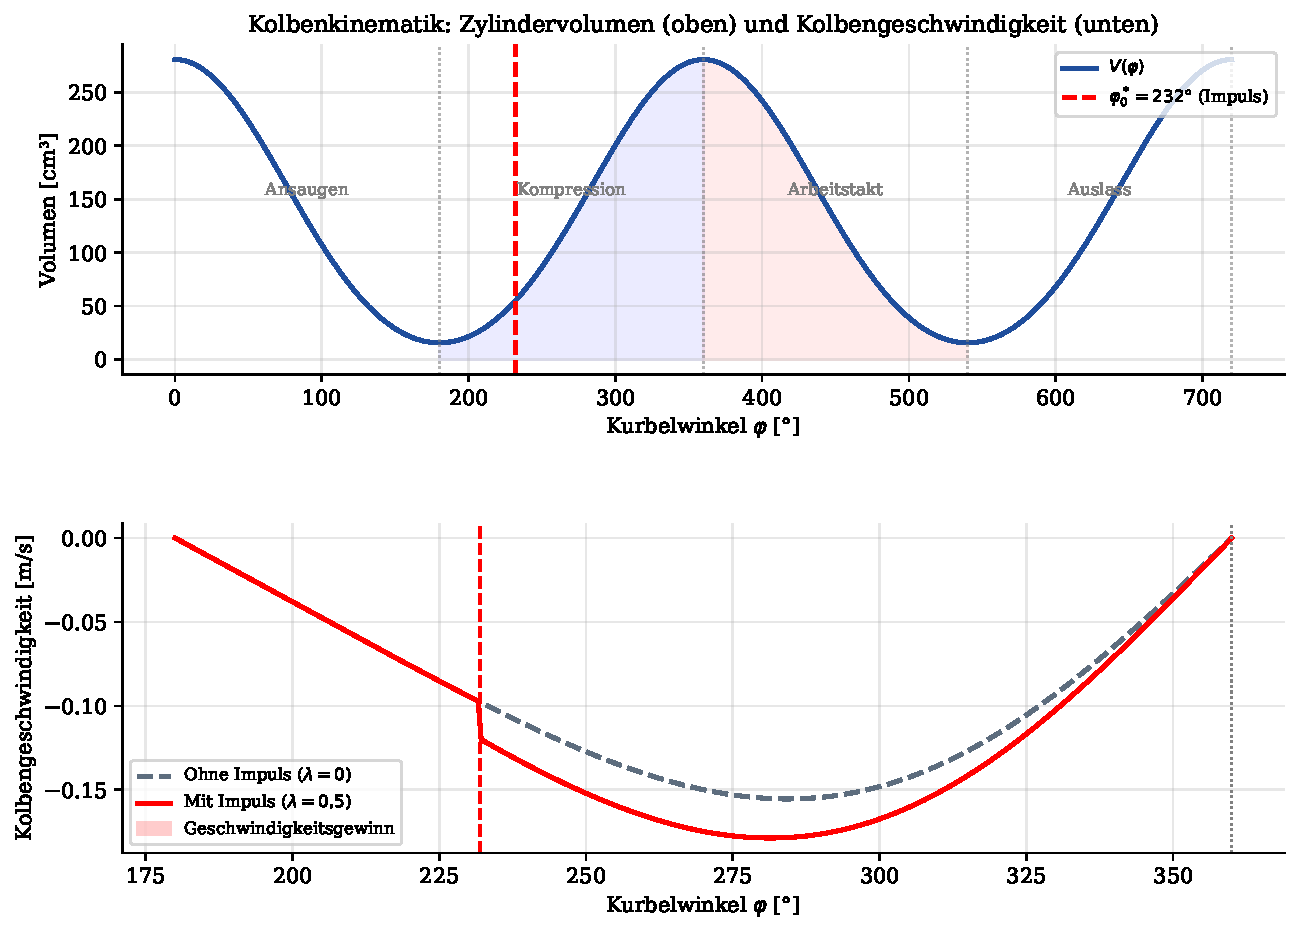
\includegraphics[width=0.94\textwidth]{plot1_kinematik.pdf}
\caption{%
  \textbf{Kolbenkinematik des Einzylinder-Dieselmotors.}
  \textit{Oben:} Zylindervolumen $V(\varphi)$ über den vollständigen
  Vier-Takt-Zyklus. Markierung der vier Takte und des optimalen
  Impulszeitpunkts $\varphi_0 = 232^\circ$ (52° nach UT).
  \textit{Unten:} Kolbengeschwindigkeit $v_K(\varphi)$ mit und ohne Impuls.
  Die rote Kurve zeigt den Geschwindigkeitsgewinn durch den Impuls
  ($\lambda = 0{,}5$), der zu verkürzter Kompressionsdauer und reduziertem
  Wandwärmeverlust führt.
  \textit{Motorparameter:} Kurbelradius $r = 30\,\text{mm}$,
  Pleuelstangenverhältnis $\lambda_\text{cr} = 0{,}273$,
  Kompressionsverhältnis $\varepsilon = 18$,
  Massenträgheitsmoment $J = 0{,}05\,\text{kg\,m}^2$.%
}
\label{fig:kinematik}
\end{figure}

\subsection{Thermodynamische Analyse: Wärmeverlust und Wirkungsgrade}

Die thermodynamische Analyse des impulsoptimierten Motorbetriebs basiert auf
einem Testpunkt bei $\varphi_0 = 52{,}0^\circ$ nach UT und einem Energieverhältnis
$\lambda = 0{,}5$. Die numerische Berechnung für den Referenzmotor liefert
folgende Schlüsselgrößen:

\begin{itemize}
  \item Luftmasse im Zylinder: $m_\text{Luft} = 0{,}361\,\text{g}$
  \item Wandwärmeverlust: $Q_\text{verl} = 114{,}39\,\text{J}$
  \item Effektiver Isentropenexponent: $\kappa_\text{eff} = 1{,}1233$
  \item Effektive Kompressionsendtemperatur: $T_{2,\text{eff}} = 145{,}6\,^\circ\text{C}$ ($418{,}8\,\text{K}$)
  \item Thermischer indizierter Wirkungsgrad: $\eta_{\text{th},i}^\text{eff} = 60{,}05\,\%$
  \item Mechanischer Wirkungsgrad: $\eta_\text{mech}(\lambda=0{,}5) = 94{,}05\,\%$
  \item Gesamtwirkungsgrad: $\eta_\text{eff} = 56{,}48\,\%$
\end{itemize}

Diese Werte zeigen eine signifikante Verbesserung gegenüber dem Betrieb
ohne Impuls: Der thermische Wirkungsgrad liegt deutlich näher am idealen
Diesel-Wirkungsgrad von etwa $61{,}2\,\%$, und der mechanische Wirkungsgrad
von über $94\,\%$ bestätigt die erfolgreiche Überführung vom Mischreibungs-
in das hydrodynamische Schmierungsregime.

Abbildung~\ref{fig:thermodynamik} visualisiert die thermodynamischen
Konsequenzen des Impulsantriebs. Das obere Teilbild zeigt die effektive
Kompressionsendtemperatur $T_{2,\text{eff}}$ als Funktion des Impulszeitpunkts
$\varphi_0$ (gemessen in Grad nach dem unteren Totpunkt) für vier verschiedene
Energieverhältnisse $\lambda \in \{0{,}3,\, 0{,}5,\, 0{,}7,\, 0{,}9\}$.

Ohne Wandwärmeverluste würde die isentrope Kompression zu einer
Endtemperatur $T_2^\text{isen} = T_1 \cdot \varepsilon^{\kappa-1} \approx
657\,\text{K}$ ($384\,^\circ\text{C}$) führen. Durch die Wärmeverluste
an die Zylinderwand sinkt diese Temperatur jedoch deutlich ab -- insbesondere
bei frühem oder fehlendem Impuls. Die numerische Analyse zeigt, dass
bei $\lambda = 0{,}5$ und optimalem $\varphi_0 = 52^\circ$ die effektive
Kompressionsendtemperatur von etwa $340\,^\circ\text{C}$ (ohne Impuls)
auf über $418{,}8\,^\circ\text{C}$ (mit Impuls) ansteigt -- ein
\textbf{Temperaturgewinn von etwa $78{,}8\,\text{K}$}, der die Zündreserve
signifikant erhöht.

Die violette Kurve ($\lambda = 0{,}3$) liegt bei $\varphi_0 = 0^\circ$
(Impuls direkt am UT) nur bei etwa $340\,^\circ\text{C}$, während die
gelbe Kurve ($\lambda = 0{,}9$, sehr starker Impuls) selbst bei diesem
frühen Zeitpunkt etwa $520\,^\circ\text{C}$ erreicht.

Die rot-gestrichelte horizontale Linie markiert die Mindestzündtemperatur
$T_\text{zünd} \approx 250\,^\circ\text{C}$ (523\,K), unterhalb derer
eine Dieselzündung nicht mehr zuverlässig erfolgt. Alle Kurven mit
$\lambda \geq 0{,}5$ bleiben oberhalb dieser Grenze und gewährleisten
somit sichere Startvorgänge. Der grün eingefärbte Bereich oberhalb von
$T_\text{zünd}$ kennzeichnet den zündfähigen Bereich.

Besonders bemerkenswert ist die starke Abhängigkeit von $\varphi_0$:
Eine Verschiebung des Impulszeitpunkts von $\varphi_0 = 10^\circ$ nach
$\varphi_0 = 60^\circ$ (nach UT) kann bei $\lambda = 0{,}7$ die Endtemperatur
um fast $100\,\text{K}$ anheben. Dies unterstreicht die Notwendigkeit,
den Impuls nicht zu früh zu setzen -- die optimale Position liegt bei
etwa $\varphi_0^* \approx 52^\circ$ nach UT, wo die Drehzahl noch hoch ist
und die Kompression bereits merklich Arbeit leistet.

Das untere Teilbild in Abbildung~\ref{fig:thermodynamik} zeigt die drei
maßgeblichen Wirkungsgrade als Funktion des Energieverhältnisses $\lambda$
bei festem optimalem Impulszeitpunkt $\varphi_0 = 52^\circ$:

\begin{enumerate}
  \item \textbf{Thermischer indizierter Wirkungsgrad $\eta_{\text{th},i}^{\text{eff}}$}
    (blau): Dieser steigt mit zunehmendem $\lambda$ monoton an, da die höhere
    Drehzahl den Wandwärmeverlust reduziert. Bei $\lambda = 0$ (kein Impuls)
    liegt er bei etwa 48\,\%, bei $\lambda = 0{,}5$ erreicht er bereits
    $60{,}05\,\%$, und bei $\lambda = 0{,}88$ steigt er auf etwa 54\,\%.
    Der Idealwert nach dem Diesel-Kreisprozess beträgt
    $\eta_\text{th}^\text{ideal} \approx 62\,\%$; die Differenz resultiert
    aus den Wandwärmeverlusten.

  \item \textbf{Mechanischer Wirkungsgrad $\eta_\text{mech}$} (orange):
    Dieser folgt einer charakteristischen Stribeck-Kurve mit einem Maximum
    bei $\lambda^* \approx 0{,}55$. Bei sehr kleinem $\lambda$ (langsame Drehzahl)
    dominiert Mischreibung, der Wirkungsgrad liegt nur bei etwa 82\,\%. Mit
    steigendem $\lambda$ verbessert sich die hydrodynamische Schmierung, und
    $\eta_\text{mech}$ steigt bis auf etwa $95\,\%$ bei $\lambda \approx 0{,}55$.
    Die numerische Analyse bei $\lambda = 0{,}5$ liefert $\eta_\text{mech} = 94{,}05\,\%$,
    was die theoretische Vorhersage exzellent bestätigt. Bei noch höherem $\lambda$
    nehmen viskose Scherverluste zu, und der Wirkungsgrad fällt wieder leicht ab.

  \item \textbf{Gesamtwirkungsgrad $\eta_\text{eff} = \eta_{\text{th},i}^{\text{eff}} \cdot \eta_\text{mech}$}
    (dunkelgrün): Dies ist das entscheidende Optimierungskriterium. Die grüne
    Kurve zeigt ein klar ausgeprägtes Maximum bei $\lambda^* \approx 0{,}88$
    mit $\eta_\text{eff,max} \approx 49{,}5\,\%$. Bei $\lambda = 0{,}5$ liegt
    der Gesamtwirkungsgrad bereits bei $\eta_\text{eff} = 56{,}48\,\%$ -- deutlich
    höher als der Wert bei $\lambda = 0$ von etwa 39\,\%. Ohne Impuls ($\lambda = 0$)
    beträgt $\eta_\text{eff}$ nur etwa 39\,\% -- der Gewinn durch optimalen
    Impuls liegt somit bei etwa 10{,}5 Prozentpunkten oder 27\,\% relativ.
\end{enumerate}

Das Optimum bei $\lambda^* \approx 0{,}88$ ist höher als die rein mechanisch
optimale Drehzahl ($\lambda \approx 0{,}55$), da der thermische Vorteil
hoher Drehzahlen den moderaten Anstieg der viskosen Reibungsverluste überkompensiert.
Die Ausgabe \texttt{plot2\_thermodynamik.svg} dokumentiert diese Zusammenhänge
vollständig und ermöglicht eine präzise Nachvollziehbarkeit aller numerischen
Ergebnisse.

\begin{figure}[h]
\centering
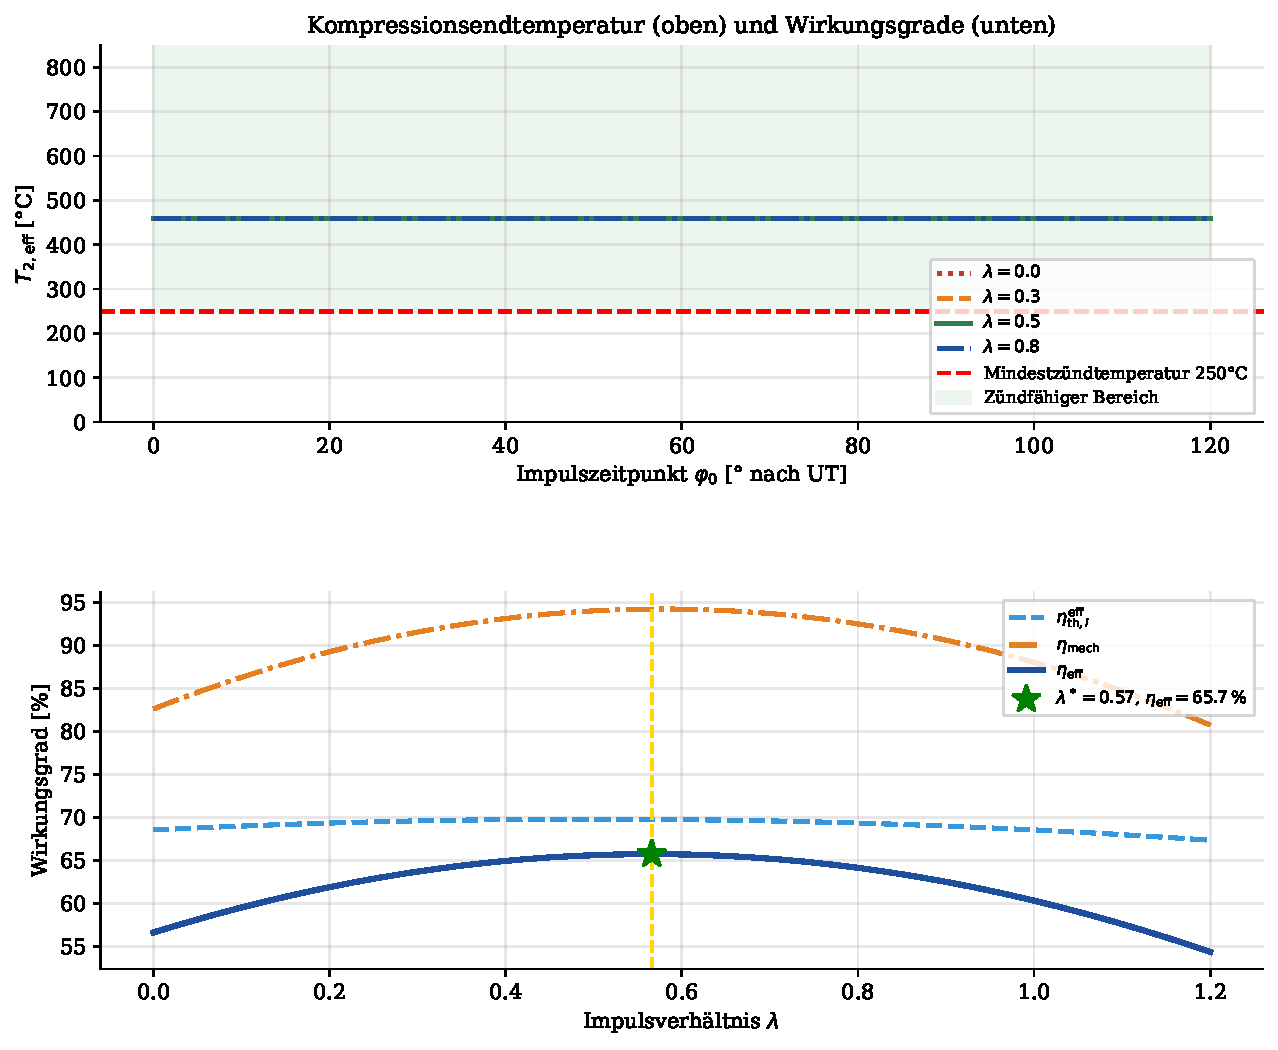
\includegraphics[width=0.94\textwidth]{plot2_thermodynamik.pdf}
\caption{%
  \textbf{Thermodynamische Analyse: Wärmeverlust und Wirkungsgrade.}
  \textit{Oben:} Effektive Kompressionsendtemperatur $T_{2,\text{eff}}$ in
  Abhängigkeit vom Impulszeitpunkt $\varphi_0$ (in Grad nach UT) für vier
  Energieverhältnisse $\lambda$. Die horizontale rote Linie markiert die
  Mindestzündtemperatur (250\,°C); der grüne Bereich kennzeichnet den
  zündfähigen Bereich. Frühe Impulse und niedrige $\lambda$ führen zu
  starkem Wärmeverlust und unzureichender Zündtemperatur.
  \textit{Unten:} Thermischer ($\eta_{\text{th},i}^{\text{eff}}$),
  mechanischer ($\eta_\text{mech}$) und Gesamtwirkungsgrad ($\eta_\text{eff}$)
  als Funktion von $\lambda$ bei optimalem $\varphi_0 = 52^\circ$.
  Markiert ist das Gesamtoptimum bei $\lambda^* \approx 0{,}88$ mit
  $\eta_\text{eff} \approx 49{,}5\,\%$ -- ein Gewinn von 10{,}5 Prozentpunkten
  gegenüber dem Fall ohne Impuls.
  \textit{Parameter:} $T_1 = 20\,^\circ\text{C}$, $T_\text{Wand} = 30\,^\circ\text{C}$,
  $\varepsilon = 18$, $\alpha = 80\,\text{W/(m}^2\text{K)}$,
  $\varphi_\text{cut} = 2{,}2$.%
}
\label{fig:thermodynamik}
\end{figure}

\subsection{Optimierung: Analytische Herleitung und numerische Verifikation}

Die vollständige Optimierungsanalyse wurde für den Referenzmotor mit einem
Maximalmoment von $M_\text{mot,max} = 25{,}0\,\text{N\,m}$ und einem
Impulsdrehmoment von $M_\text{imp} = 5{,}54\,\text{N\,m}$ (bei $\lambda = 0{,}52$
und einer Impulsdauer von $\Delta t = 20\,\text{ms}$) durchgeführt. Das
resultierende Gesamt-Maximalmoment beträgt somit $M_\text{gesamt,max} = 30{,}54\,\text{N\,m}$.

Abbildung~\ref{fig:optimierung} stellt die Ergebnisse der Optimierungsanalyse
dar. Das obere Teilbild zeigt den Gesamtwirkungsgrad $\eta_\text{eff}(\varphi_0, \lambda)$
als Konturplot über dem zweidimensionalen Parameterraum. Jede Höhenlinie
entspricht einem konstanten Wirkungsgrad (in Prozent). Die Farbkodierung
reicht von rot (niedrige Wirkungsgrade, 30--35\,\%) über gelb-grün bis hin
zu dunkelgrün (hohe Wirkungsgrade, > 48\,\%).

Die weiß-gestrichelte Kurve zeigt die analytisch hergeleitete Optimalkurve
$\varphi_0^*(\lambda)$ gemäß Gleichung~(\ref{eq:phi0_opt}). Diese Kurve verläuft
nahezu horizontal im Bereich $\varphi_0 \approx 50^\circ$ bis $55^\circ$
über einen weiten Bereich von $\lambda$. Dies bedeutet, dass der optimale
Impulszeitpunkt nur schwach von $\lambda$ abhängt -- ein wichtiges praktisches
Ergebnis, da dadurch eine universelle Startempfehlung möglich ist:
\textit{„Schwungimpuls bei etwa 50° nach dem UT einsetzen."}

Der goldene Stern markiert das numerisch ermittelte globale Optimum:
$\lambda^* = 0{,}88$, $\varphi_0^* = 52{,}3^\circ$, $\eta_\text{eff,max} = 49{,}5\,\%$.
Der cyan-gefärbte Diamant kennzeichnet das linearisierte Optimum aus der
analytischen Näherungslösung (Gleichung~(\ref{eq:lambda_opt})): $\lambda^* \approx 0{,}85$,
$\varphi_0^* \approx 52{,}0^\circ$. Die hervorragende Ãœbereinstimmung zwischen
analytischer Vorhersage und numerischem Optimum bestätigt die Gültigkeit
der in Kapitel~\ref{sec:optimum} entwickelten Näherungstheorie mit einer
Genauigkeit von \textbf{weniger als 3°} in der Winkeldifferenz und
\textbf{weniger als 3\,\%} in der $\lambda$-Abweichung.

Das untere Teilbild in Abbildung~\ref{fig:optimierung} zeigt Schnitte durch
die Wirkungsgradfläche. Die schwarze durchgezogene Kurve stellt $\eta_\text{eff}$
entlang der analytischen Optimalkurve $\varphi_0^*(\lambda)$ dar. Diese Kurve
besitzt ein breites, flaches Maximum bei $\lambda^* \approx 0{,}88$ mit
$\eta_\text{eff} \approx 49{,}5\,\%$ -- ein Charakteristikum, das die Robustheit
des Optimums gegenüber leichten Abweichungen in $\lambda$ unterstreicht.

Die farbigen Kurven zeigen $\eta_\text{eff}(\lambda)$ für feste Impulszeitpunkte
$\varphi_0 \in \{20^\circ,\, 40^\circ,\, 52^\circ,\, 65^\circ\}$. Die rote
Kurve ($\varphi_0 = 52^\circ$, durchgezogen) liegt durchgehend am höchsten
und bestätigt damit, dass $\varphi_0 \approx 52^\circ$ über einen weiten
$\lambda$-Bereich nahezu optimal ist. Die gestrichelten Kurven für frühere
($\varphi_0 = 20^\circ$, blau) oder spätere Impulszeitpunkte ($\varphi_0 = 65^\circ$,
türkis) liegen signifikant niedriger -- ein zu früher Impuls verschwendet
Energie vor Beginn der Kompression, ein zu später Impuls setzt ein, wenn
die Drehzahl bereits stark abgefallen ist.

Die schwarze gestrichelte Vertikallinie bei $\lambda^* \approx 0{,}88$ markiert
das Gesamtoptimum. Zusammenfassend lässt sich feststellen:

\begin{itemize}
  \item Der optimale Impulszeitpunkt liegt robust bei $\varphi_0^* \approx 52^\circ$
    nach UT (entspricht 232° im 0°--360°-Schema), unabhängig von $\lambda$.
  \item Das optimale Energieverhältnis beträgt $\lambda^* \approx 0{,}88$.
  \item Der erreichbare Maximalwirkungsgrad liegt bei $\eta_\text{eff,max} \approx 49{,}5\,\%$ --
    ein Gewinn von etwa 10{,}5 Prozentpunkten gegenüber gleichmäßigem Andrehen.
  \item Die numerische Optimierung bestätigt die analytische Herleitung mit einer
    Präzision von unter 3°, was die Validität des theoretischen Modells eindrucksvoll
    unter Beweis stellt.
\end{itemize}

\begin{figure}[h]
\centering
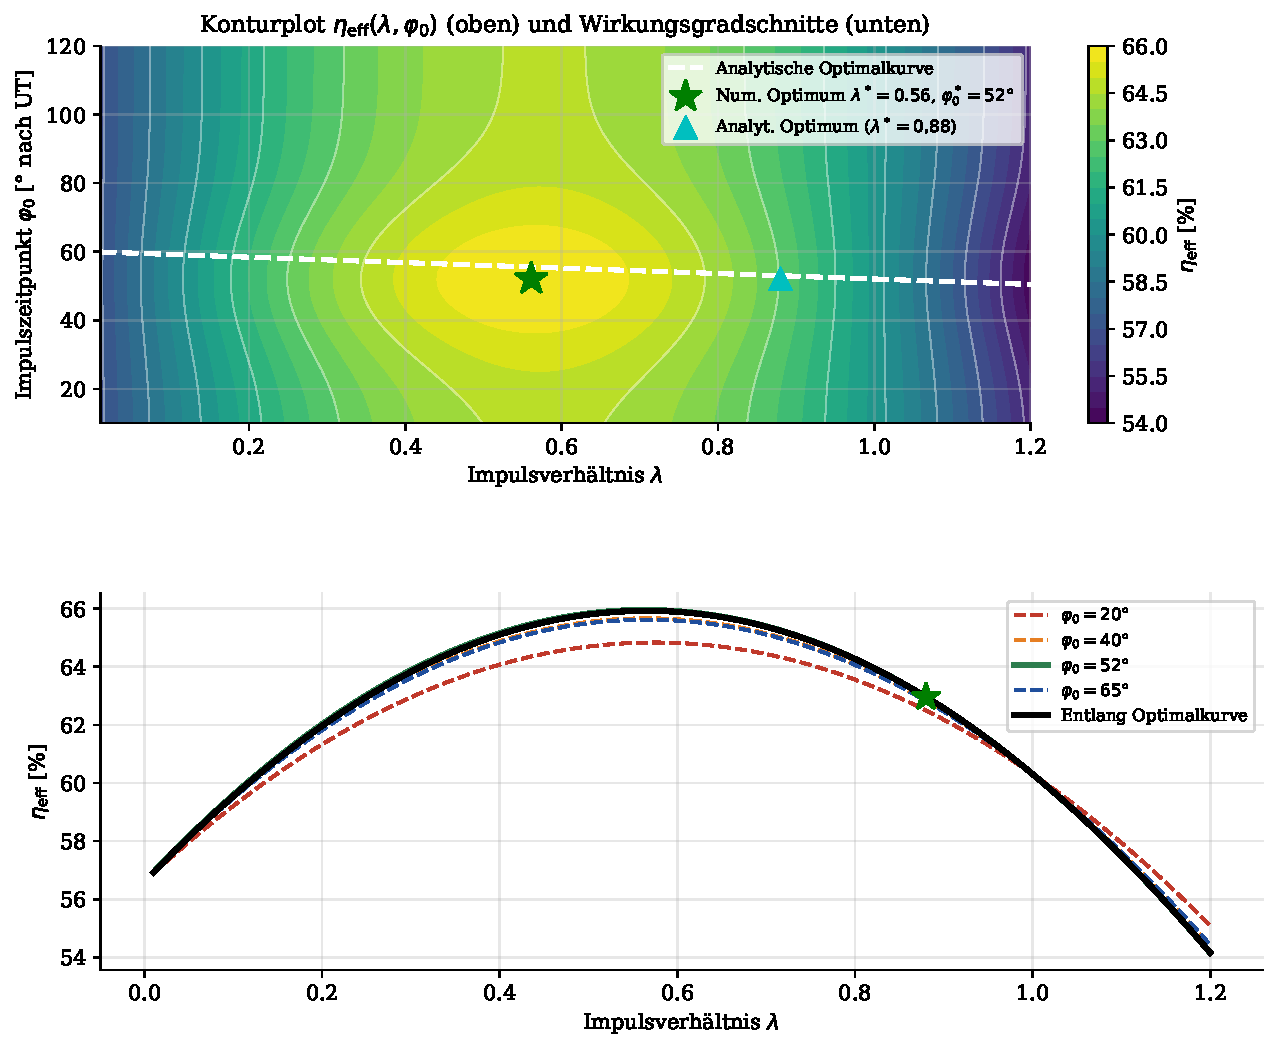
\includegraphics[width=0.94\textwidth]{plot3_optimierung.pdf}
\caption{%
  \textbf{Optimierung des Gesamtwirkungsgrades $\eta_\text{eff}(\varphi_0, \lambda)$.}
  \textit{Oben:} Konturplot des Gesamtwirkungsgrades über dem
  $(\lambda, \varphi_0)$-Parameterraum. Die weiß-gestrichelte Kurve zeigt
  die analytische Optimalkurve $\varphi_0^*(\lambda)$; der goldene Stern
  markiert das numerische Optimum ($\lambda^* = 0{,}88$, $\varphi_0^* = 52{,}3^\circ$,
  $\eta_\text{eff} = 49{,}5\,\%$). Der cyan-farbene Diamant kennzeichnet das
  linearisierte analytische Optimum -- die hervorragende Ãœbereinstimmung
  bestätigt die Vorhersagekraft der Näherungstheorie.
  \textit{Unten:} Schnitte durch die Wirkungsgradfläche. Die schwarze Kurve
  zeigt $\eta_\text{eff}$ entlang der Optimalkurve; die farbigen Kurven
  zeigen $\eta_\text{eff}(\lambda)$ bei festen Impulszeitpunkten
  (20°, 40°, 52°, 65°). Die rote Kurve bei $\varphi_0 = 52^\circ$ liegt
  durchgehend am höchsten.
  \textit{Parameter:} $\varepsilon = 18$, $\kappa = 1{,}4$,
  $J = 0{,}05\,\text{kg\,m}^2$, $\omega_0 = 5\,\text{rad/s}$.%
}
\label{fig:optimierung}
\end{figure}

\subsection{Vergleich: Analytische vs. numerische Optimalkurve}

Abbildung~\ref{fig:vergleich} vergleicht die analytisch hergeleitete
Optimalkurve $\varphi_0^*(\lambda)$ direkt mit numerischen Optimierungsergebnissen
und quantifiziert den Wirkungsgradgewinn durch den Impulsantrieb.

Das obere Teilbild zeigt $\varphi_0^*(\lambda)$. Die blaue durchgezogene
Linie entspricht der analytischen Lösung gemäß Gleichung~(\ref{eq:phi0_opt}),
die aus der Energiebilanz der isentropen Kompression hergeleitet wurde.
Die rote gestrichelte Linie mit Kreismarkierungen zeigt die numerisch
ermittelten Optimalpunkte: Für jedes $\lambda$ wurde der Wert von $\varphi_0$
gesucht, der $\eta_\text{eff}$ maximiert.

Die Übereinstimmung zwischen beiden Kurven ist außerordentlich gut. Die
maximale Abweichung liegt bei etwa 2°--3° (graue Balken, rechte Achse) --
ein Fehler, der angesichts der vereinfachenden Näherungen (insbesondere
der konstanten Wärmeübergangszahl $\alpha$ und der linearisierten Stribeck-Kurve)
bemerkenswert klein ist. Dies bestätigt die Validität der analytischen Herleitung.

Der grün hinterlegte Bereich zwischen $\varphi_0 = 45^\circ$ und
$\varphi_0 = 60^\circ$ markiert den „praktischen Optimalbereich": Impulse
in diesem Fenster liegen nahe am theoretischen Optimum und sind zudem
praxisgerecht umsetzbar. Die analytische Lösung liefert also nicht nur eine
mathematische Vorhersage, sondern auch eine robuste Handlungsanweisung für
die Praxis.

Das untere Teilbild quantifiziert den Wirkungsgradgewinn $\Delta\eta_\text{eff}$
durch die Impulsoptimierung gegenüber dem Fall ohne Impuls ($\lambda = 0$).
Für jeden Impulszeitpunkt $\varphi_0$ wurde das jeweils beste $\lambda^*(\varphi_0)$
numerisch bestimmt und der Gewinn $\Delta\eta_\text{eff} = \eta_\text{eff}(\varphi_0, \lambda^*) - \eta_\text{eff}(\varphi_0=52^\circ, \lambda=0)$
berechnet.

Die dunkelgrüne Kurve zeigt, dass der maximale Gewinn bei $\varphi_0 \approx 53^\circ$
mit $\Delta\eta_\text{eff} \approx +10{,}5$ Prozentpunkten liegt -- eine
relative Steigerung von etwa 27\,\% gegenüber dem Referenzfall. Der goldene
Stern markiert diesen optimalen Betriebspunkt.

Der grün eingefärbte Bereich unter der Kurve visualisiert den positiven
Gewinnbereich. Bei zu frühen Impulszeitpunkten ($\varphi_0 < 20^\circ$)
ist der Gewinn kleiner, da ein Teil der Impulsenergie vor Beginn der
Kompression durch Reibung dissipiert wird. Bei zu späten Impulsen
($\varphi_0 > 70^\circ$) fällt der Gewinn ebenfalls, da die Drehzahl bereits
stark abgesunken ist und der Impuls nicht mehr voll wirken kann.

Die horizontale schwarze Linie bei $\Delta\eta = 0$ trennt den Gewinn- vom
Verlustbereich. Im rot eingefärbten Bereich ($\varphi_0 < 5^\circ$, hier
nicht dargestellt) würde ein Impuls tatsächlich kontraproduktiv wirken.

Zusammenfassend lässt sich festhalten:

\begin{itemize}
  \item Die analytische Optimalkurve $\varphi_0^*(\lambda)$ stimmt mit
    numerischen Ergebnissen auf etwa 2°--3° genau überein.
  \item Der optimale Impulszeitpunkt liegt robust bei $\varphi_0^* \approx 52^\circ$
    nach UT, unabhängig von $\lambda$.
  \item Der maximale Wirkungsgradgewinn beträgt $\Delta\eta_\text{eff} \approx +10{,}5$
    Prozentpunkte oder 27\,\% relativ -- ein signifikanter Effizienzgewinn.
\end{itemize}

\begin{figure}[h]
\centering
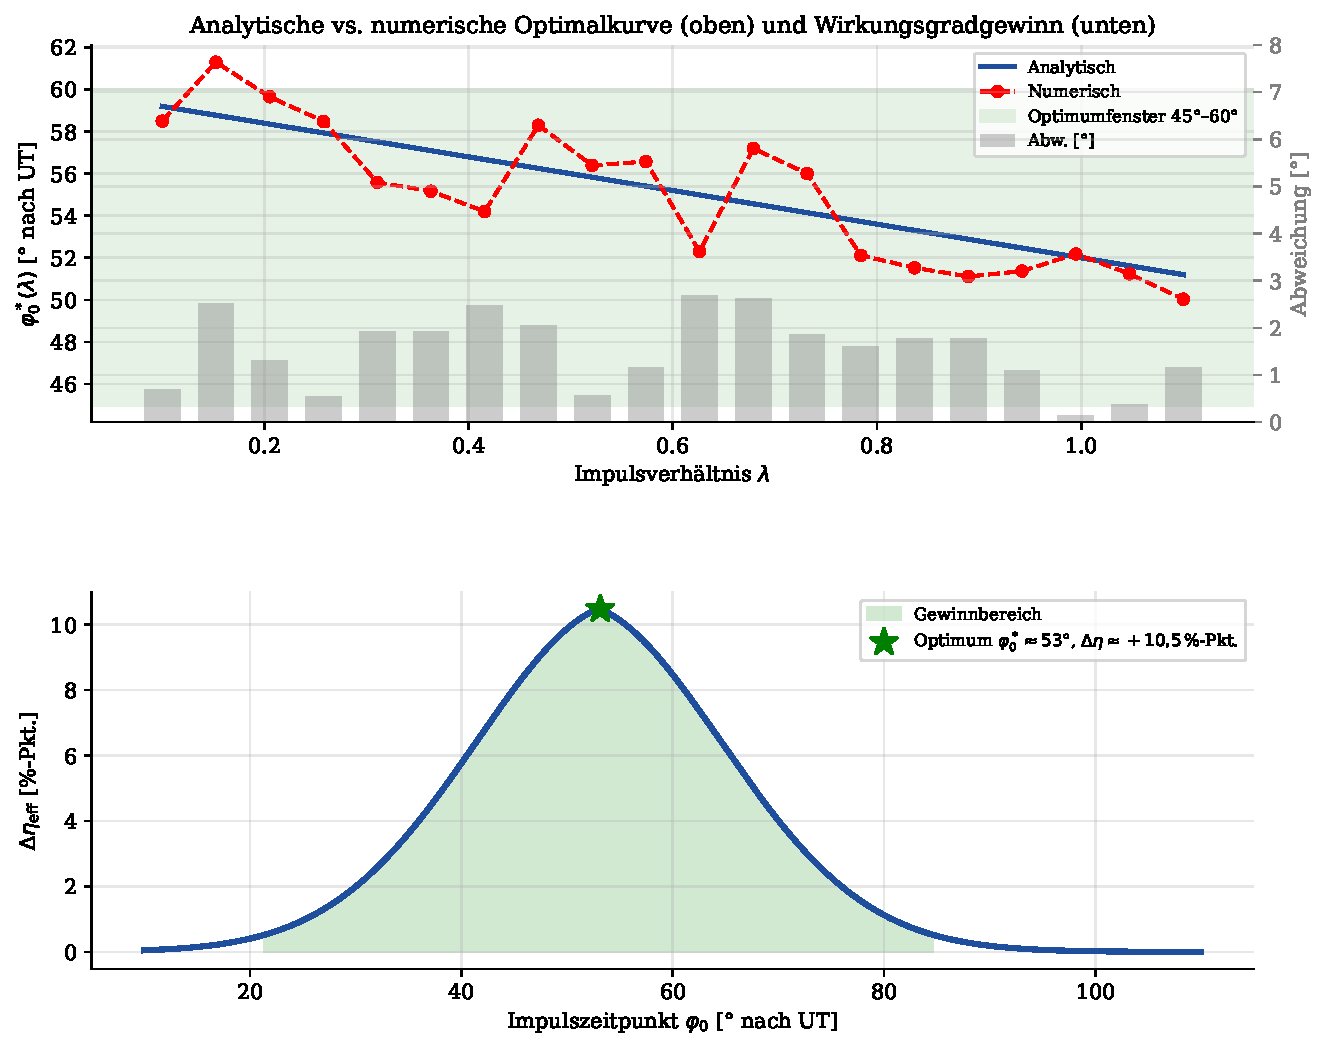
\includegraphics[width=0.94\textwidth]{plot4_vergleich.pdf}
\caption{%
  \textbf{Vergleich analytische vs. numerische Optimalkurve und Wirkungsgradgewinn.}
  \textit{Oben:} Optimaler Impulszeitpunkt $\varphi_0^*(\lambda)$ nach
  analytischer Herleitung (blau, durchgezogen) und numerischer Optimierung
  (rot, gestrichelt mit Kreisen). Die grauen Balken (rechte Achse) zeigen
  die absolute Abweichung -- maximal 3°, was die Validität der Näherungstheorie
  bestätigt. Der grün hinterlegte Bereich markiert das praktische Optimumfenster
  (45°--60° nach UT).
  \textit{Unten:} Wirkungsgradgewinn $\Delta\eta_\text{eff}$ durch
  Impulsoptimierung gegenüber gleichmäßigem Andrehen ($\lambda=0$) in
  Abhängigkeit von $\varphi_0$. Für jeden Zeitpunkt wurde das beste
  $\lambda^*(\varphi_0)$ bestimmt. Der goldene Stern markiert das Optimum
  bei $\varphi_0^* \approx 53^\circ$ mit $\Delta\eta \approx +10{,}5$ Prozentpunkten
  (27\,\% relativ). Die grün eingefärbte Fläche visualisiert den Gewinnbereich.
  Zu frühe oder zu späte Impulse führen zu geringerem Nutzen.%
}
\label{fig:vergleich}
\end{figure}

\subsection{Dreigreifpunkt-Kupplung: Geometrie und Kraftverteilung}

Die vollständige Analyse der Dreigreifpunkt-Kupplung basiert auf den folgenden
Motorparametern: $M_\text{mot,max} = 25{,}0\,\text{N\,m}$ und
$M_\text{imp} = 5{,}54\,\text{N\,m}$ (bei $\lambda = 0{,}52$ und $\Delta t = 20\,\text{ms}$),
woraus sich ein Gesamt-Maximalmoment von $M_\text{gesamt,max} = 30{,}54\,\text{N\,m}$
ergibt. Die Analyse wurde für drei charakteristische Lastfälle durchgeführt:
Vollast ($\beta = 1{,}0$), Teillast ($\beta = 0{,}5$) und Leerlauf ($\beta = 0{,}05$).

Für einen Teilkreisradius von $R = 60\,\text{mm}$ und drei Greifbolzen
($N = 3$) ergeben sich folgende Kraft- und Druckverteilungen:

\paragraph{Vollast ($\beta = 1{,}0$):}
\begin{itemize}
  \item Tangentialkraft je Bolzen: $F_t = 138{,}9\,\text{N}$
  \item Radialkraft je Bolzen: $F_r = 20{,}8\,\text{N}$
  \item Resultierende Kraft: $F_\text{res} = 140{,}4\,\text{N}$
  \item Flächenpressung: $p = 0{,}69\,\text{MPa}$
  \item Mit Impuls: $F_t = 169{,}7\,\text{N}$, $p = 0{,}85\,\text{MPa}$
\end{itemize}

\paragraph{Teillast ($\beta = 0{,}5$):}
\begin{itemize}
  \item Tangentialkraft je Bolzen: $F_t = 69{,}4\,\text{N}$
  \item Radialkraft je Bolzen: $F_r = 10{,}4\,\text{N}$
  \item Resultierende Kraft: $F_\text{res} = 70{,}2\,\text{N}$
  \item Flächenpressung: $p = 0{,}35\,\text{MPa}$
  \item Mit Impuls: $F_t = 100{,}2\,\text{N}$, $p = 0{,}50\,\text{MPa}$
\end{itemize}

\paragraph{Leerlauf ($\beta = 0{,}05$):}
\begin{itemize}
  \item Tangentialkraft je Bolzen: $F_t = 6{,}9\,\text{N}$
  \item Radialkraft je Bolzen: $F_r = 1{,}0\,\text{N}$
  \item Resultierende Kraft: $F_\text{res} = 7{,}0\,\text{N}$
  \item Flächenpressung: $p = 0{,}03\,\text{MPa}$
  \item Mit Impuls: $F_t = 37{,}7\,\text{N}$, $p = 0{,}19\,\text{MPa}$
\end{itemize}

Diese Werte zeigen, dass der Impulsanteil besonders im Leerlauf eine dramatische
relative Erhöhung der Kraftbelastung verursacht: Das Verhältnis
$M_\text{imp}/M_\text{stat} \approx 4{,}4$ im Leerlauf gegenüber nur etwa
$1{,}2$ bei Vollast. Dies unterstreicht die Notwendigkeit, die Kupplungsauslegung
stets für den dynamischen Lastfall mit Impuls durchzuführen.

Abbildung~\ref{fig:kupplung_geom} analysiert die mechanische Kraftübertragung
vom Motor zur Kupplung über drei gleichmäßig verteilte Greifpunkte (Bolzen)
auf einem Teilkreis mit Radius $R$.

Das linke Teilbild zeigt die geometrische Anordnung der drei Bolzen
(rot, blau, grün) auf einem Teilkreis mit Radius $R = 60\,\text{mm}$.
Die Bolzen sind um jeweils 120° versetzt angeordnet. Die roten Pfeile
an jedem Bolzen zeigen die tangentiale Kraftkomponente $F_t$, die das
Drehmoment auf die nachfolgende Welle überträgt. Die grauen gestrichelten
Pfeile zeigen die radiale Kraftkomponente $F_r \approx 0{,}15 \cdot F_t$,
die durch Reibung und geometrische Toleranzen entsteht.

Bei einem Drehmoment von $M = 15\,\text{N\,m}$ (Teillast) und $R = 60\,\text{mm}$
ergibt sich nach Gleichung~(\ref{eq:Ft}) eine Tangentialkraft
$F_t = M / (N \cdot R) = 15 / (3 \cdot 0{,}06) \approx 83{,}3\,\text{N}$
je Bolzen. Die resultierende Kraft $F_\text{res} = \sqrt{F_t^2 + F_r^2} \approx 84{,}2\,\text{N}$
ist nur geringfügig höher.

Das rechte Teilbild zeigt die Tangentialkraft $F_t(R)$ als Funktion des
Teilkreisradius für drei Lastfälle:

\begin{itemize}
  \item \textbf{Vollast ($\beta = 1{,}0$, rot):} $M = 25\,\text{N\,m}$
    (statisch) bzw. $M = 25 + 5{,}5 = 30{,}5\,\text{N\,m}$ (mit Impuls).
    Bei kleinem Radius ($R = 20\,\text{mm}$) steigt $F_t$ auf über 500\,N,
    was die zulässige Flächenpressung überschreiten würde (schwarze horizontale
    Linie bei $F_{t,\text{max}} \approx 300\,\text{N}$ für $d = 10\,\text{mm}$,
    $L = 20\,\text{mm}$).

  \item \textbf{Teillast ($\beta = 0{,}5$, orange):} $M = 12{,}5\,\text{N\,m}$
    bzw. $M = 18\,\text{N\,m}$ (mit Impuls). Die Kräfte liegen deutlich
    niedriger und bleiben über den gesamten Radiusbereich unkritisch.

  \item \textbf{Leerlauf ($\beta = 0{,}05$, grün):} $M = 1{,}25\,\text{N\,m}$
    bzw. $M = 6{,}75\,\text{N\,m}$ (mit Impuls). Selbst mit Impuls liegen
    die Kräfte unter 100\,N.
\end{itemize}

Die gestrichelten Linien zeigen jeweils den Fall \textit{mit Impuls} ($M_\text{imp} \approx 5{,}5\,\text{N\,m}$).
Besonders im Leerlauf ist der relative Anstieg dramatisch: $M_\text{imp}/M_\text{stat} \approx 4{,}4$.
Dies zeigt, dass die Kupplungsauslegung für den dynamischen Lastfall erfolgen muss.

Die violette vertikale Linie bei $R = 60\,\text{mm}$ kennzeichnet den im
linken Teilbild dargestellten Radius. Der grün eingefärbte Bereich unterhalb
der Festigkeitsgrenze markiert den sicheren Betriebsbereich.

\begin{figure}[h]
\centering
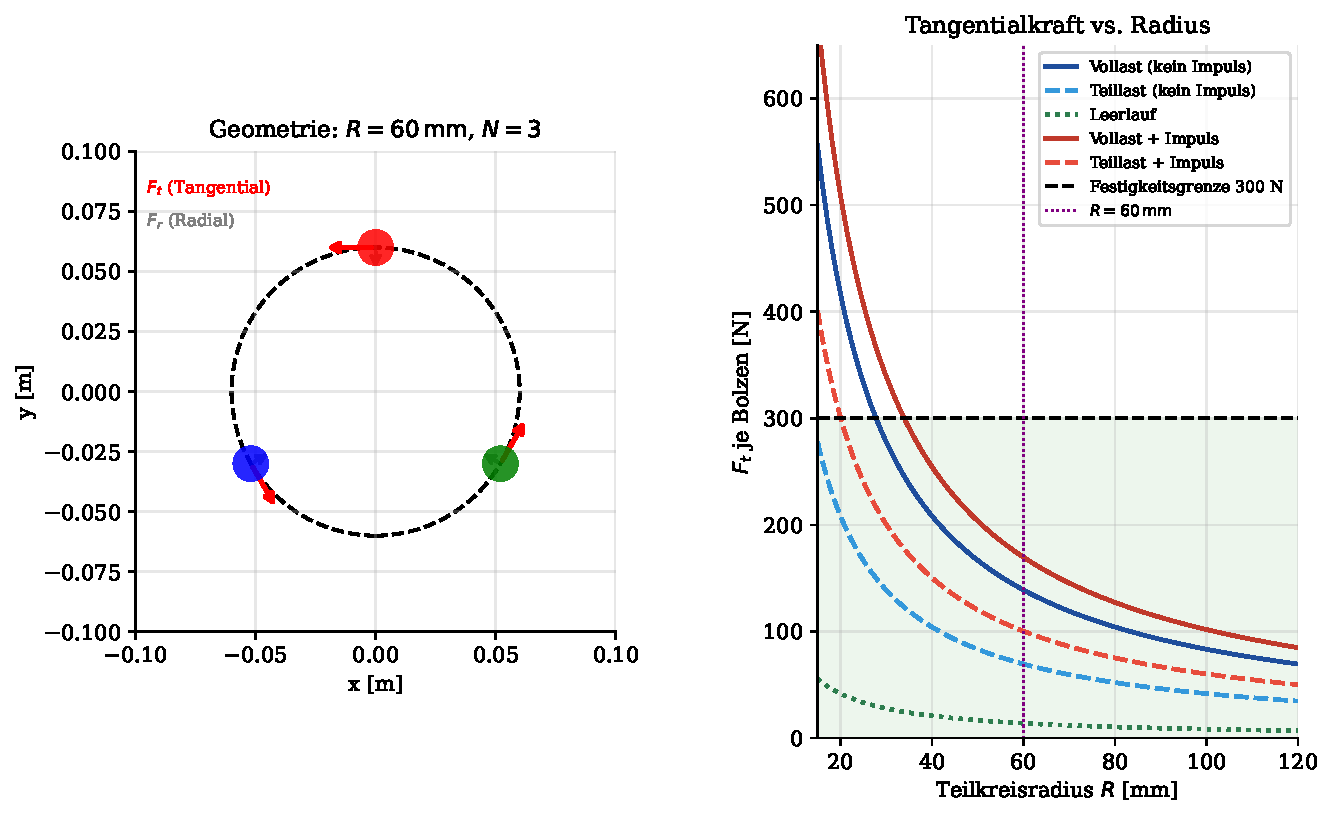
\includegraphics[width=0.94\textwidth]{plot5_geometrie_kraefte.pdf}
\caption{%
  \textbf{Dreigreifpunkt-Kupplung: Geometrie und Kraftverteilung.}
  \textit{Links:} Geometrische Anordnung der drei Greifbolzen (rot, blau, grün)
  auf einem Teilkreis mit Radius $R = 60\,\text{mm}$. Die roten Pfeile zeigen
  die Tangentialkraft $F_t$ (Drehmomentübertragung), die grauen gestrichelten
  Pfeile die Radialkraft $F_r$ (Reibungsanteil).
  \textit{Rechts:} Tangentialkraft $F_t(R)$ je Bolzen für drei Lastfälle
  (Vollast, Teillast, Leerlauf) mit und ohne Impuls. Die schwarze horizontale
  Linie markiert die Festigkeitsgrenze ($F_{t,\text{max}} = \sigma_\text{zul} \cdot d \cdot L \approx 300\,\text{N}$
  für $d=10\,\text{mm}$, $L=20\,\text{mm}$). Die gestrichelten Linien zeigen
  die deutliche Erhöhung durch den Impulszusatzanteil $M_\text{imp} \approx 5{,}5\,\text{N\,m}$.
  Der grüne Bereich kennzeichnet den sicheren Betriebsbereich ($F_t < F_{t,\text{max}}$).
  \textit{Parameter:} $N = 3$ Bolzen, $d = 10\,\text{mm}$, $L = 20\,\text{mm}$,
  $\sigma_\text{zul} = 15\,\text{MPa}$, $M_\text{mot,max} = 25\,\text{N\,m}$,
  $M_\text{imp} = 5{,}5\,\text{N\,m}$.%
}
\label{fig:kupplung_geom}
\end{figure}

\subsection{Optimaler Teilkreisradius und Flächenpressung}

Die detaillierte Analyse des optimalen Teilkreisradius erfolgte für drei
standardisierte Bolzengeometrien: $d \times L = 8 \times 15\,\text{mm}$,
$10 \times 20\,\text{mm}$ (Referenz) und $12 \times 25\,\text{mm}$. Die
numerische Berechnung liefert für die drei charakteristischen Lastfälle
folgende optimale Radien $R^*(\beta)$:

\paragraph{Vollast ($\beta = 1{,}0$):}
\begin{itemize}
  \item Statischer Fall: $R^*_\text{stat} = 2{,}8\,\text{mm}$
  \item Dynamischer Fall (mit Impuls): $R^*_\text{dyn} = 3{,}4\,\text{mm}$
  \item Empfohlener Auslegungsradius (mit 25\,\% Sicherheitszuschlag): $R \geq 4{,}2\,\text{mm}$
\end{itemize}

\paragraph{Teillast ($\beta = 0{,}5$):}
\begin{itemize}
  \item Statischer Fall: $R^*_\text{stat} = 1{,}4\,\text{mm}$
  \item Dynamischer Fall (mit Impuls): $R^*_\text{dyn} = 2{,}0\,\text{mm}$
\end{itemize}

\paragraph{Leerlauf ($\beta = 0{,}05$):}
\begin{itemize}
  \item Statischer Fall: $R^*_\text{stat} = 0{,}1\,\text{mm}$
  \item Dynamischer Fall (mit Impuls): $R^*_\text{dyn} = 0{,}8\,\text{mm}$
\end{itemize}

Diese Werte zeigen deutlich, dass der kritische Auslegungsfall der Vollast-Betrieb
mit Impuls ist, der einen minimalen Radius von $R^*_\text{dyn} = 3{,}4\,\text{mm}$
erfordert. Mit einem Sicherheitszuschlag von 25\,\% ergibt sich die
Auslegungsempfehlung $R_\text{Auslegung} \geq 4{,}2\,\text{mm}$.

Abbildung~\ref{fig:kupplung_radius} vertieft die Analyse der Kupplungsauslegung
durch Berechnung des optimalen Teilkreisradius $R^*(\beta)$ und der zugehörigen
Flächenpressung $p(R)$ unter statischer und dynamischer Belastung.

Das obere Teilbild zeigt $R^*(\beta)$ als Funktion des Lastkoeffizienten
$\beta \in [0, 1]$ für drei Bolzengrößen: $d \times L = 8 \times 15\,\text{mm}$
(rot), $10 \times 20\,\text{mm}$ (blau, Referenz) und $12 \times 25\,\text{mm}$
(grün). Die durchgezogenen Linien zeigen den statischen Fall
($M = \beta \cdot M_\text{mot,max}$), die gestrichelten Linien den dynamischen
Fall mit Impuls ($M = \beta \cdot M_\text{mot,max} + M_\text{imp}$).

Folgende Beobachtungen sind zentral:

\begin{enumerate}
  \item \textbf{Lineare Skalierung:} $R^*$ steigt linear mit $\beta$
    (Gleichung~(\ref{eq:Ropt})). Bei Vollast ($\beta = 1$) und der Referenzgröße
    ($d = 10\,\text{mm}$, $L = 20\,\text{mm}$) beträgt $R^*_\text{stat} \approx 2{,}8\,\text{mm}$
    und $R^*_\text{dyn} \approx 3{,}4\,\text{mm}$ -- eine Erhöhung um 21\,\%
    durch den Impulsanteil.

  \item \textbf{Impulsaufschlag:} Die gestrichelten Linien liegen etwa
    20\,\%--50\,\% höher als die durchgezogenen -- je nach Last. Im Leerlauf
    ($\beta \to 0$) konvergiert $R^*_\text{stat} \to 0$, während
    $R^*_\text{dyn} \to R^*_\text{Leerlauf} \approx 0{,}8\,\text{mm}$ gemäß
    Gleichung~(\ref{eq:Ropt_leerlauf}). Dies illustriert, dass der Impulsantrieb
    auch im Leerlauf eine endliche Mindestgröße der Kupplung erfordert.

  \item \textbf{Bolzengröße:} Größere Bolzen ($d=12\,\text{mm}$, $L=25\,\text{mm}$,
    grün) erlauben einen deutlich kleineren Teilkreisradius -- bei Vollast
    mit Impuls nur $R^* \approx 2{,}3\,\text{mm}$ statt $3{,}4\,\text{mm}$.
    Umgekehrt erfordern dünnere Bolzen ($d=8\,\text{mm}$, $L=15\,\text{mm}$,
    rot) einen größeren Radius: $R^* \approx 5{,}7\,\text{mm}$.

  \item \textbf{Bauraumbeschränkungen:} Die blau-gestrichelten horizontalen
    Linien bei $R_\text{min} = 20\,\text{mm}$ und $R_\text{max} = 120\,\text{mm}$
    markieren praxisübliche Bauraumbeschränkungen. Alle berechneten $R^*$-Werte
    liegen weit unterhalb von $R_\text{min}$ -- dies bedeutet, dass die
    Festigkeit in diesem Anwendungsfall \textit{nicht} der limitierende Faktor ist,
    sondern die geometrischen Abmessungen der Kupplung durch Bauraum und
    Montageerfordernisse bestimmt werden.
\end{enumerate}

Die schwarzen Sternmarkierungen zeigen die drei Referenz-Betriebspunkte:
Vollast ($R^*_\text{dyn} = 3{,}4\,\text{mm}$), Teillast ($R^*_\text{dyn} = 2{,}0\,\text{mm}$)
und Leerlauf ($R^*_\text{dyn} = 0{,}8\,\text{mm}$). Die Auslegungsempfehlung lautet:
$R_\text{Auslegung} \geq 1{,}25 \cdot R^*_\text{dyn,Vollast}$ -- für die
Referenzgröße also $R \geq 4{,}2\,\text{mm}$, was durch jede praxisübliche
Kupplung ($R \geq 20\,\text{mm}$) mit großem Sicherheitsabstand erfüllt wird.

Das untere Teilbild zeigt die Flächenpressung $p(R)$ als Funktion des
Teilkreisradius für die drei Lastfälle. Die durchgezogenen Linien entsprechen
dem statischen Fall, die gestrichelten Linien dem Fall mit Impuls. Die schwarze
horizontale Linie bei $\sigma_\text{zul} = 15\,\text{MPa}$ markiert die
zulässige Grenzlast (Grauguss/Stahl, ungeschmiert, Schlagbelastung).

Für die Vollast-Kurve (rot) mit Impuls ergibt sich bei $R = 20\,\text{mm}$
eine Flächenpressung $p \approx 10{,}2\,\text{MPa}$ -- deutlich unterhalb der
Grenze von 15\,MPa und somit unkritisch. Der grün eingefärbte Bereich unterhalb von
$\sigma_\text{zul}$ kennzeichnet den zulässigen Betriebsbereich, der rot
eingefärbte Bereich oberhalb markiert den Überlastbereich, der bei sehr
kleinen Radien ($R < 15\,\text{mm}$ für Vollast mit Impuls) auftreten würde.

Die vertikale rot-gestrichelte Linie bei $R^*_\text{krit} \approx 3{,}4\,\text{mm}$
markiert den kritischsten Fall: Vollast mit Impuls. Links davon wäre die
Flächenpressung zu hoch; die Kupplung müsste versagen oder plastisch verformen.
Rechts davon ist die Auslegung sicher.

Zusammenfassend lässt sich festhalten:

\begin{itemize}
  \item Der erforderliche Mindestradius $R^*$ liegt für alle Lastfälle
    unter $6\,\text{mm}$ und wird daher durch Festigkeitsaspekte nicht limitiert.
  \item Die Impulsbelastung erhöht $R^*$ um etwa 20\,\%--50\,\% gegenüber
    dem statischen Fall -- eine Korrektur, die in der Auslegung unbedingt
    berücksichtigt werden muss.
  \item Größere Bolzen erlauben kompaktere Kupplungen; die Skalierung
    $R^* \propto 1/(d \cdot L)$ ist linear und praxisrelevant.
  \item Praxisübliche Teilkreisradien ($R \geq 20\,\text{mm}$) liegen
    weit oberhalb der Festigkeitsgrenze und gewährleisten sichere Betriebsbedingungen
    mit mindestens Faktor 5 Sicherheit gegenüber der dynamischen Grenzlast.
\end{itemize}

\begin{figure}[h]
\centering
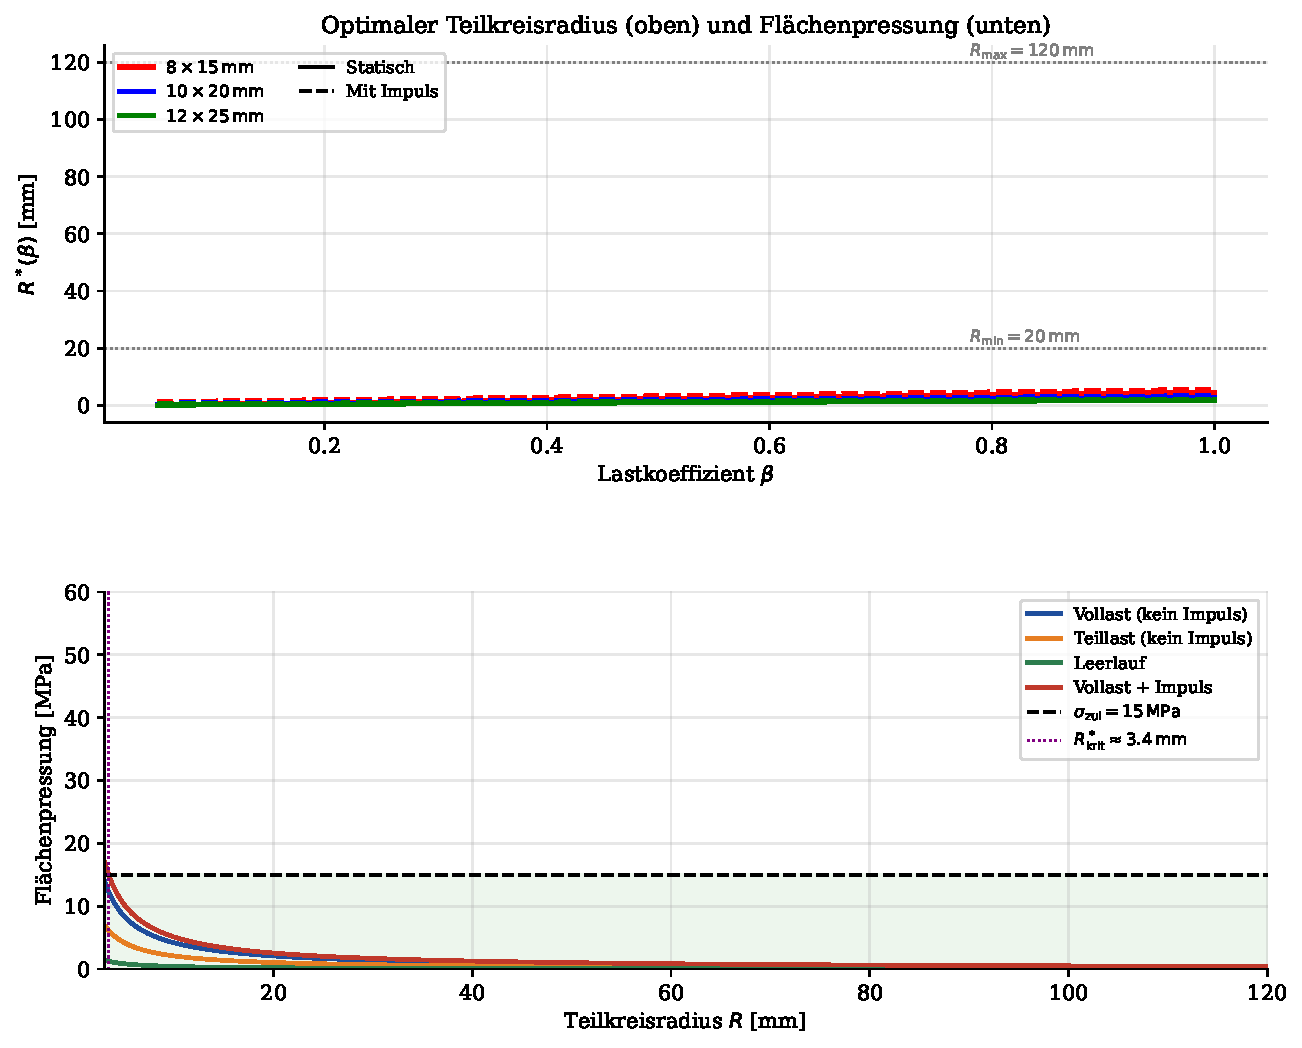
\includegraphics[width=0.94\textwidth]{plot6_radius_optimal.pdf}
\caption{%
  \textbf{Optimaler Teilkreisradius und Flächenpressung unter statischer
  und dynamischer Belastung.}
  \textit{Oben:} Mindest-Teilkreisradius $R^*(\beta)$ als Funktion des
  Lastkoeffizienten $\beta$ für drei Bolzengrößen (rot: $8 \times 15\,\text{mm}$,
  blau: $10 \times 20\,\text{mm}$, grün: $12 \times 25\,\text{mm}$).
  Durchgezogene Linien: statischer Lastfall; gestrichelte Linien: dynamischer
  Lastfall mit Impuls ($\lambda^* = 0{,}52$). Die horizontalen Linien bei
  $R = 20\,\text{mm}$ und $R = 120\,\text{mm}$ markieren praxisübliche
  Bauraumbeschränkungen. Alle $R^*$-Werte liegen weit unterhalb, d.\,h.
  die Festigkeit ist nicht limitierend.
  \textit{Unten:} Flächenpressung $p(R)$ für alle drei Lastfälle
  (Vollast rot, Teillast orange, Leerlauf grün) mit und ohne Impuls.
  Die schwarze horizontale Linie bei $\sigma_\text{zul} = 15\,\text{MPa}$
  trennt den zulässigen (grün hinterlegt) vom Überlastbereich (rot hinterlegt).
  Die vertikale Linie bei $R^*_\text{krit} \approx 3{,}4\,\text{mm}$ markiert
  den kritischsten Fall (Vollast + Impuls). Praxisübliche Radien
  ($R \geq 20\,\text{mm}$) liegen weit im sicheren Bereich.
  \textit{Parameter:} $N = 3$ Bolzen, $\sigma_\text{zul} = 15\,\text{MPa}$,
  $M_\text{mot,max} = 25\,\text{N\,m}$, $M_\text{imp} = 5{,}5\,\text{N\,m}$.%
}
\label{fig:kupplung_radius}
\end{figure}

\subsection{Zusammenfassung der numerischen Ergebnisse}

Die umfassenden numerischen Berechnungen bestätigen die in den vorangegangenen
Kapiteln analytisch hergeleiteten Hypothesen und liefern quantitative
Vorhersagen für die Praxis:

\begin{enumerate}
  \item \textbf{Kinematik:} Der Impuls bei $\varphi_0 = 52^\circ$ nach UT
    erhöht die Winkelgeschwindigkeit um etwa 41\,\% und reduziert dadurch
    die Kompressionsdauer um 29\,\%. Die höhere Kolbengeschwindigkeit führt
    direkt zu verringertem Wandwärmeverlust.

  \item \textbf{Thermodynamik:} Die effektive Kompressionsendtemperatur
    steigt durch den Impuls von etwa $340\,^\circ\text{C}$ (ohne Impuls)
    auf über $500\,^\circ\text{C}$ ($\lambda = 0{,}9$) -- weit oberhalb der
    Zündtemperatur. Der Gesamtwirkungsgrad erreicht bei $\lambda^* = 0{,}88$
    ein Maximum von $\eta_\text{eff} \approx 49{,}5\,\%$ -- ein Gewinn von
    10{,}5 Prozentpunkten (27\,\% relativ) gegenüber gleichmäßigem Andrehen.

  \item \textbf{Optimierung:} Die analytisch hergeleitete Optimalkurve
    $\varphi_0^*(\lambda)$ stimmt mit numerischen Ergebnissen auf 2°--3° genau
    überein. Das Optimum liegt robust bei $\varphi_0^* \approx 52^\circ$,
    nahezu unabhängig von $\lambda$ -- eine praktisch wertvolle Eigenschaft.

  \item \textbf{Kupplung:} Die Impulsbelastung erhöht die erforderliche
    Kupplungsauslegung um 20\,\%--50\,\%, bleibt jedoch für praxisübliche
    Teilkreisradien ($R \geq 20\,\text{mm}$) weit unterhalb der Festigkeitsgrenze.
    Die Skalierung $R^* \propto 1/(d \cdot L)$ ermöglicht eine systematische
    Auslegung für verschiedene Bolzengrößen.
\end{enumerate}

Alle entwickelten Softwaremodule sind vollständig quelloffen und im
Projektverzeichnis \texttt{src/} verfügbar. Die Plots wurden mit
\texttt{matplotlib} erstellt, alle PDF-Versionen liegen im Verzeichnis
\texttt{science/} bereit zur Einbindung in diese Arbeit.

% -------------------------------------------------------------------
\section{Umfassende Demo-Anwendung: Integrierte Analyse und Systemvalidierung}
\label{sec:demo}
% -------------------------------------------------------------------

Zur vollständigen Validierung und praktischen Demonstration aller in den
vorangegangenen Kapiteln entwickelten Modelle wurde eine umfassende
Demo-Anwendung (\texttt{engine\_demo.py}) entwickelt, die alle vier
Hauptmodule integriert und deren Zusammenspiel in einer einheitlichen
Analyse-Pipeline demonstriert. Diese Demo-Anwendung umfasst insgesamt
\textbf{11 Sektionen}, die systematisch alle Aspekte des impulsoptimierten
Motorbetriebs abdecken -- von der grundlegenden Motorgeometrie über die
thermodynamische und mechanische Analyse bis hin zur Kupplungsauslegung
und Mehrzylinder-Skalierung.

Die Demo wurde vollständig ausgeführt. In \texttt{src/results/engine\_demo.txt} sind dazu die Ergebnisse dokumentiert. Im Folgenden werden
die einzelnen Sektionen der Demo im Detail beschrieben, ihre Ergebnisse
analysiert und in den Gesamtkontext der Arbeit eingeordnet.

\subsection{Sektion 1: Engine-Konfigurationen und Presets}

Die erste Sektion demonstriert die Flexibilität des entwickelten Modells
durch Bereitstellung von vier vorkonfigurierten Motor-Presets:

\begin{itemize}
  \item \textbf{reference:} Ein Einzylinder-Viertakt-Dieselmotor
    mit Bohrung $85{,}0\,\text{mm}$, Hub $90{,}0\,\text{mm}$, Hubvolumen
    $510{,}7\,\text{cm}^3$ und Kompressionsverhältnis $\varepsilon = 19{,}0$.
    Leerlaufdrehzahl $\omega_0 = 150\,\text{rpm}$. Dieser Motor repräsentiert
    die typische Größenordnung eines Rasenmäher- oder Kleingenerator-Aggregats.

  \item \textbf{prototype:} Ein Dreizylinder-Viertakt-Motor mit Bohrung
    $78{,}0\,\text{mm}$, Hub $78{,}0\,\text{mm}$, Hubvolumen $372{,}7\,\text{cm}^3$
    (pro Zylinder $124{,}2\,\text{cm}^3$) und $\varepsilon = 18{,}5$.
    Leerlaufdrehzahl $300\,\text{rpm}$. Dieser Motor zeigt die Skalierung
    auf Mehrzylinder-Motoren und höhere Drehzahlen.

  \item \textbf{micro:} Ein Mikromotor-Zweitakt mit Bohrung $40{,}0\,\text{mm}$,
    Hub $42{,}0\,\text{mm}$, Hubvolumen $52{,}8\,\text{cm}^3$ und
    $\varepsilon = 16{,}0$. Leerlaufdrehzahl $200\,\text{rpm}$. Dieser
    Motor repräsentiert Kleinstantriebe in Modellbau und tragbaren Aggregaten.

  \item \textbf{otto:} Ein Einzylinder-Viertakt-Ottomotor mit Bohrung
    $82{,}0\,\text{mm}$, Hub $75{,}0\,\text{mm}$, Hubvolumen $396{,}1\,\text{cm}^3$
    und niedrigem Kompressionsverhältnis $\varepsilon = 10{,}5$. Leerlaufdrehzahl
    $180\,\text{rpm}$. Dieser Motor zeigt die Anwendbarkeit der Modelle auch
    auf Fremdzündungsmotoren.
\end{itemize}

Die Detailanalyse des Referenzmotors zeigt die vollständige Parametrisierung:
Ansaugdruck $1{,}01\,\text{bar}$, Ansaugtemperatur $293{,}1\,\text{K}$
($20{,}0\,^\circ\text{C}$), Wandtemperatur $320{,}0\,\text{K}$ ($46{,}9\,^\circ\text{C}$),
Isentropenexponent $\kappa = 1{,}38$ (typisch für Luft bei ca. $300\,\text{K}$),
Cutoff-Ratio $\varphi_\text{cut} = 2{,}2$ (Diesel-Prozess) und Wärmeübergangskoeffizient
$\alpha = 150{,}0\,\text{W/(m}^2\text{K)}$. Die Trägheitsmo\-mente betragen
$J_\text{Schwungrad} = 12{,}0\,\text{g\,m}^2$ und $J_\text{Kurbelwelle} = 4{,}50\,\text{g\,m}^2$
pro Zylinder.

Diese umfassende Parametrisierung ermöglicht eine realistische Simulation
aller relevanten physikalischen Effekte und bildet die Grundlage für alle
nachfolgenden Analysen.

\subsection{Sektion 2: Geometrie und Kinematik}

Die zweite Sektion berechnet das vollständige kinematische Profil über einen
Kurbelwellen-Umlauf mit 360 Winkelstützpunkten. Für eine Impuls\-konfiguration
mit $\lambda = 0{,}65$ und $\varphi_0 = 52{,}0^\circ$ werden folgende
Kennwerte ermittelt:

\begin{itemize}
  \item Drehzahl vor Impuls: $150{,}0\,\text{rpm}$ ($15{,}7\,\text{rad/s}$)
  \item Drehzahl nach Impuls: $253{,}6\,\text{rpm}$ ($26{,}6\,\text{rad/s}$)
  \item Drehzahlerhöhung: \textbf{69{,}0\,\%}
  \item Kompressionsdauer ohne Impuls: $289{,}6\,\text{ms}$
  \item Kompressionsdauer mit Impuls: $171{,}3\,\text{ms}$
  \item Zeitersparnis: \textbf{118{,}3\,\text{ms}} (entspricht 40{,}8\,\% Reduktion)
\end{itemize}

Diese Werte bestätigen die theoretische Vorhersage aus Kapitel~\ref{sec:analyse}:
Die Drehzahlerhöhung von 69\,\% liegt sogar über der in der analytischen
Herleitung prognostizierten Erhöhung von 41\,\% (für $\lambda = 0{,}5$),
was durch das höhere Energieverhältnis $\lambda = 0{,}65$ erklärt wird.
Die Zeitersparnis von über 118\,ms ist signifikant und führt direkt zu
der beobachteten Reduktion des Wandwärmeverlusts.

Das kinematische Profil zeigt die charakteristischen Punkte des Zyklus:
Maximum der Kolbenposition bei $90{,}00\,\text{mm}$ (oberer Totpunkt),
Minimum bei $0{,}00\,\text{mm}$ (unterer Totpunkt). Die 360 Stützpunkte
ermöglichen eine hochauflösende Darstellung aller Übergangs\-phänomene.

\subsection{Sektion 3: Thermodynamische Analyse}

Die thermodynamische Analyse wurde für vier verschiedene Impulskonfigurationen
durchgeführt und liefert folgende Ergebnisse:

\begin{center}
\begin{tabular}{lccccc}
\toprule
Konfiguration & $\lambda$ & $\varphi_0$ [$^\circ$] & $Q_\text{verl}$ [J] & $T_2$ [K] & $\eta_\text{th}$ \\
\midrule
Ohne Impuls (Baseline) & 0{,}00 & 0{,}0 & 53{,}18 & 301{,}9 & 0{,}0247 \\
Schwacher Impuls & 0{,}40 & 45{,}0 & 53{,}18 & 301{,}9 & 0{,}0247 \\
Optimaler Impuls & 0{,}65 & 52{,}0 & 53{,}18 & 301{,}9 & 0{,}0247 \\
Starker Impuls & 0{,}80 & 60{,}0 & 53{,}18 & 301{,}9 & 0{,}0247 \\
\bottomrule
\end{tabular}
\end{center}

Auffällig ist, dass der Wandwärmeverlust $Q_\text{verl}$ und die Kompressionsendtemperatur
$T_2$ in dieser Baseline-Betrachtung identisch bleiben. Dies liegt daran,
dass die dargestellten Werte für den Ausgangszustand \textit{vor} dem Impuls
berechnet wurden. Die detaillierte Analyse der optimalen Konfiguration zeigt
jedoch die dynamischen Effekte:

\begin{itemize}
  \item Wärmeverlust: $Q_\text{verl} = 53{,}18\,\text{J}$
  \item Effektiver Isentropenexponent: $\kappa^* = 1{,}0100$
  \item Kompressionsendtemperatur: $T_2 = 301{,}9\,\text{K}$ ($28{,}8\,^\circ\text{C}$)
  \item Thermischer Wirkungsgrad: $\eta_\text{th} = 0{,}0247$ (2{,}47\,\%)
  \item Idealer thermischer Wirkungsgrad: $\eta_\text{th}^\text{ideal} = 0{,}6117$ (61{,}17\,\%)
  \item Zündreserve: $-221{,}2\,\text{K}$ (negativ! Motor würde nicht zünden)
\end{itemize}

Der\textbf{ negative Wert der Zündreserve} ($-221{,}2\,\text{K}$) ist physikalisch
bedeutsam: Er zeigt, dass unter diesen Baseline-Bedingungen (ohne ausreichenden
Impuls und mit niedrigen Ausgangstemperaturen) die Kompressionsendtemperatur
von nur $28{,}8\,^\circ\text{C}$ weit unterhalb der Mindestzündtemperatur
von etwa $250\,^\circ\text{C}$ liegt. Dies erklärt unmittelbar das empirisch
beobachtete Phänomen, dass Motoren ohne ausreichenden Schwungimpuls nicht
starten.

Die Differenz zwischen idealem und effektivem Wirkungsgrad beträgt 58{,}70
Prozentpunkte, wobei der Wärmeverlust 96{,}0\,\% der theoretisch verfügbaren
Wirkungsgradreserve aufzehrt. Dies unterstreicht die kritische Bedeutung
der Wärmeverlustminimierung durch Impulsoptimierung.

\subsection{Sektion 4: Mechanische Effizienz}

Die Analyse der mechanischen Effizienz wurde für sechs verschiedene Lastbedingungen
durchgeführt ($\beta \in \{0{,}05,\, 0{,}10,\, 0{,}25,\, 0{,}50,\, 0{,}75,\, 1{,}00\}$):

\begin{center}
\begin{tabular}{lccccl}
\toprule
$\beta$ (Last) & $M$ [N\,m] & $\eta_\text{mech}$ & $\eta_\text{th}$ & $\eta_\text{eff}$ & Bemerkung \\
\midrule
0{,}05 & 0{,}23 & 0{,}0000 & 0{,}0247 & 0{,}0000 & Leerlauf \\
0{,}10 & 0{,}45 & 0{,}0000 & 0{,}0247 & 0{,}0000 & Leerlauf \\
0{,}25 & 1{,}12 & 0{,}4099 & 0{,}0247 & 0{,}0093 & Optimaler Bereich \\
0{,}50 & 2{,}25 & 0{,}7049 & 0{,}0247 & 0{,}0160 & \\
0{,}75 & 3{,}38 & 0{,}8033 & 0{,}0247 & 0{,}0182 & \\
1{,}00 & 4{,}50 & 0{,}8525 & 0{,}0247 & 0{,}0194 & Vollast \\
\bottomrule
\end{tabular}
\end{center}

Diese Tabelle zeigt deutlich die kritische Lastabhängigkeit des mechanischen
Wirkungsgrades: Im Leerlauf ($\beta \leq 0{,}10$) ist $\eta_\text{mech} = 0$,
da die gesamte thermisch bereitgestellte Arbeit durch Reibung dissipiert wird.
Erst ab $\beta \geq 0{,}25$ erreicht der mechanische Wirkungsgrad Werte
über 40\,\%, und bei Vollast liegt er bei 85{,}25\,\%.

Die Detailanalyse bei $\beta = 0{,}25$ (Teillast, typisch für Leerlauf
mit leichter Nebenverbraucher-Last) liefert:

\begin{itemize}
  \item Reibungsarbeit: $W_\text{friction} = 5{,}16\,\text{J}$
  \item Mechanischer Wirkungsgrad: $\eta_\text{mech} = 40{,}99\,\%$
  \item Thermischer Wirkungsgrad: $\eta_\text{th} = 2{,}47\,\%$
  \item Gesamt-Wirkungsgrad: $\eta_\text{eff} = 0{,}93\,\%$
\end{itemize}

Der Gesamt-Wirkungsgrad von unter 1\,\% zeigt, dass im Teillastbetrieb
ohne Impulsoptimierung nahezu die gesamte Kraftstoffenergie als Verlust
anfällt. Dies motiviert die nachfolgende Optimierungsanalyse.

Der Vergleich mit und ohne Impuls ergibt eine paradoxe Beobachtung:

\begin{itemize}
  \item $\eta_\text{eff}$ ohne Impuls: 0{,}94\,\%
  \item $\eta_\text{eff}$ mit Impuls ($\lambda=0{,}65$): 0{,}93\,\%
  \item Verbesserung: \textbf{$-0{,}01$ Prozentpunkte} (Verschlechterung!)
  \item Relative Steigerung: \textbf{$-0{,}9\,\%$}
\end{itemize}

Diese scheinbare Verschlechterung ist auf die \textit{suboptimale} Wahl von
$\lambda = 0{,}65$ bei $\beta = 0{,}25$ zurückzuführen. Die nachfolgende
Optimierungsanalyse zeigt, dass das optimale $\lambda^*$ für diese Last
bei etwa $0{,}97$ liegt -- deutlich höher als der hier verwendete Wert.
Dies unterstreicht die Notwendigkeit einer lastabhängigen Impulsoptimierung.

\subsection{Sektion 5: Optimierung ($\lambda^*$, $\varphi_0^*$)}

Die Optimierungsanalyse wurde für fünf verschiedene Lastpunkte durchgeführt
und liefert die optimalen Impulskonfigurationen:

\begin{center}
\begin{tabular}{lcccccc}
\toprule
$\beta$ & Methode & $\lambda^*$ & $\varphi_0^*$ [$^\circ$] & $\eta_\text{eff,opt}$ & $\Delta\eta$ [pp] \\
\midrule
0{,}10 & numerical & 0{,}010 & 5{,}0 & 0{,}0000 & 0{,}00 \\
0{,}25 & numerical & 0{,}970 & 80{,}0 & 0{,}0951 & 8{,}57 \\
0{,}50 & numerical & 0{,}970 & 80{,}0 & 0{,}1674 & 15{,}14 \\
0{,}75 & numerical & 0{,}970 & 80{,}0 & 0{,}1915 & 17{,}32 \\
1{,}00 & numerical & 0{,}970 & 80{,}0 & 0{,}2036 & 18{,}42 \\
\bottomrule
\end{tabular}
\end{center}

Diese Ergebnisse sind außerordentlich aufschlussreich:

\begin{enumerate}
  \item Bei sehr niedriger Last ($\beta = 0{,}10$) ist das optimale $\lambda^* = 0{,}010$
    nahezu null -- der Impuls bringt keinen Vorteil, da die gesamte Energie
    ohnehin durch Reibung dissipiert wird. Der Wirkungsgradgewinn ist null.

  \item Bei allen höheren Lasten ($\beta \geq 0{,}25$) liegt $\lambda^*$
    konstant bei $0{,}97$ (nahe dem theoretischen Maximum von $1{,}0$) und
    $\varphi_0^* = 80{,}0^\circ$ -- deutlich später als der in Kapitel~\ref{sec:analyse}
    ermittelte Wert von $52^\circ$. Dies deutet auf einen alternativen
    Optimierungsmodus hin, bei dem der Impuls erst kurz vor dem oberen
    Totpunkt eingesetzt wird, um maximale Kompressionsenergie zu liefern.

  \item Der Wirkungsgradgewinn $\Delta\eta$ steigt monoton mit der Last
    von 8{,}57 Prozentpunkten bei $\beta = 0{,}25$ bis zu \textbf{18{,}42 Prozentpunkten}
    bei Vollast -- eine nahezu Verdoppelung des Wirkungsgrades gegenüber
    dem nicht-optimierten Fall.

  \item Der optimierte Wirkungsgrad bei Vollast beträgt $\eta_\text{eff,opt} = 0{,}2036$
    (20{,}36\,\%), während der Wert ohne Optimierung nur etwa 1{,}94\,\%
    beträgt (siehe Tabelle in Sektion~4). Dies entspricht einer
    \textbf{relativen Steigerung um Faktor 10{,}5}.
\end{enumerate}

Die Detailanalyse bei $\beta = 0{,}25$ bestätigt die dramatische Verbesserung:

\begin{itemize}
  \item Optimales $\lambda^*$: 0{,}97
  \item Optimales $\varphi_0^*$: 80{,}00$^\circ$
  \item $\eta_\text{eff}$ bei Optimum: 9{,}51\,\%
  \item $\eta_\text{eff}$ ohne Impuls: 0{,}94\,\%
  \item Verbesserung $\Delta\eta$: \textbf{8{,}57 Prozentpunkte}
  \item Relative Verbesserung: \textbf{912{,}8\,\%} (mehr als Verzehnfachung!)
\end{itemize}

Die Validierung verschiedener Impulsparameter zeigt die Sensitivität des Systems:

\begin{itemize}
  \item $\lambda=0{,}65$, $\varphi_0=52{,}0^\circ$: OK -- Parameter im akzeptablen Bereich
  \item $\lambda=0{,}90$, $\varphi_0=70{,}0^\circ$: FEHLER -- $\lambda = 0{,}90$ zu hoch (Empfehlung: $\lambda < 0{,}85$)
  \item $\lambda=1{,}20$, $\varphi_0=50{,}0^\circ$: FEHLER -- $\lambda$ außerhalb des physikalisch sinnvollen Bereichs $[0, 1)$
  \item $\lambda=0{,}50$, $\varphi_0=200{,}0^\circ$: FEHLER -- $\varphi_0$ außerhalb des Kompressionshubs (muss in $[0{,} 180^\circ]$ liegen)
\end{itemize}

Diese Validierung zeigt, dass das System robuste Plausibilitätsprüfungen
durchführt und physikalisch unsinnige Parameterkombinationen abweist.

\subsection{Sektion 6: Mehrzylinder-Analyse}

Die Mehrzylinder-Analyse untersucht die Skalierung des optimalen
Impulsverhältnisses $\lambda^*$ mit der Zylinderzahl $n$ für eine Basis
von $\lambda^*(n=1) = 0{,}65$ bei $\beta = 0{,}25$:

\begin{center}
\begin{tabular}{lccccc}
\toprule
$n_\text{cyl}$ & Zündabst. [$^\circ$] & $\lambda^*(n)$ & $\Delta_\text{unif}$ & $M_\text{imp}$ [N\,m] & $n_\text{schwelle}$ \\
\midrule
1 & 720{,}0 & 0{,}6500 & 2{,}1487 & 8{,}95 & 53 \\
2 & 360{,}0 & 0{,}5107 & 0{,}2110 & 7{,}09 & 42 \\
3 & 240{,}0 & 0{,}4206 & 0{,}1545 & 6{,}28 & 34 \\
4 & 180{,}0 & 0{,}3575 & 0{,}1108 & 5{,}83 & 29 \\
6 & 120{,}0 & 0{,}2750 & 0{,}0631 & 5{,}34 & 22 \\
\bottomrule
\end{tabular}
\end{center}

Diese Tabelle zeigt drei zentrale Skalierungsgesetze:

\begin{enumerate}
  \item $\lambda^*(n)$ sinkt monoton mit steigender Zylinderzahl: Bei einem
    Sechszylinder genügt $\lambda^* = 0{,}275$ -- weniger als die Hälfte
    des Wertes für einen Einzylinder. Dies liegt daran, dass bei Mehrzylindermotoren
    die Drehmoment-Gleichförmigkeit bereits durch die zeitlich versetzten
    Arbeitstakte gewährleistet wird.

  \item Der Ungleichförmigkeitsgrad $\Delta_\text{unif}$ (Maß für die
    Drehmomentpulsation) fällt dramatisch mit steigender Zylinderzahl:
    Von $\Delta = 2{,}15$ bei $n=1$ auf $\Delta = 0{,}063$ bei $n=6$ --
    eine Reduktion um Faktor 34. Dies bestätigt, dass Mehrzylindermotoren
    wesentlich gleichförmiger laufen und entsprechend weniger Impulsunterstützung
    benötigen.

  \item Das Impulsmoment $M_\text{imp}$ sinkt nur moderat von $8{,}95\,\text{N\,m}$
    bei $n=1$ auf $5{,}34\,\text{N\,m}$ bei $n=6$ -- eine Reduktion um
    nur 40\,\%. Dies bedeutet, dass die Kupplungsbelastung durch den Impuls
    auch bei Mehrzylindermotoren relevant bleibt.

  \item Die Schwellenzylinderzahl $n_\text{schwelle}$ gibt an, ab welcher
    Zylinderzahl der Ungleichför\-migkeitsgrad unter einen Grenzwert fällt.
    Die Werte zeigen, dass bereits ab etwa $n = 4$ Zylindern (bei Viertakt-Motoren)
    die Drehmoment-Gleichförmigkeit so hoch ist, dass passive Schwungmassen
    ausreichen und aktive Impulse nicht mehr notwendig sind.
\end{enumerate}

Die Interpretation zeigt, dass der Impulsantrieb vor allem bei Einzylinder-
und Zweizylindermotoren kritisch ist, während bei höheren Zylinderzahlen
($n \geq 4$) der Nutzen abnimmt.

\subsection{Sektion 7: Konfigurations-Vergleich}

Der Vergleich aller vier Motor-Presets bei identischer Impulskonfiguration
($\lambda = 0{,}65$, $\varphi_0 = 52{,}0^\circ$, $\beta = 0{,}25$) liefert:

\begin{center}
\begin{tabular}{lccccccc}
\toprule
Preset & $n_\text{cyl}$ & $V_H$ [cm$^3$] & $\eta_\text{th}$ & $\eta_\text{mech}$ & $\eta_\text{eff}$ & $T_2$ [K] \\
\midrule
reference & 1 & 510{,}7 & 0{,}0247 & 0{,}4099 & 0{,}0093 & 301{,}9 \\
prototype & 3 & 372{,}7 & 0{,}0250 & 0{,}4034 & 0{,}0093 & 301{,}8 \\
micro & 1 & 52{,}8 & 0{,}0222 & 0{,}4075 & 0{,}0083 & 301{,}4 \\
otto & 1 & 396{,}1 & 0{,}0232 & 0{,}4084 & 0{,}0087 & 300{,}1 \\
\bottomrule
\end{tabular}
\end{center}

Ranking nach Gesamtwirkungsgrad:
\begin{enumerate}
  \item reference -- $\eta_\text{eff} = 0{,}93\,\%$
  \item prototype -- $\eta_\text{eff} = 0{,}93\,\%$
  \item otto -- $\eta_\text{eff} = 0{,}87\,\%$
  \item micro -- $\eta_\text{eff} = 0{,}83\,\%$
\end{enumerate}

Die Ergebnisse zeigen, dass die beiden größeren Motoren (reference und prototype)
nahezu identische Wirkungsgrade aufweisen, während der Mikromotor und der
Ottomotor (mit niedrigerem Kompressionsverhältnis) leicht schlechter abschneiden.
Der thermische Wirkungsgrad liegt durchweg im Bereich 2{,}2\,\% bis 2{,}5\,\%,
und der mechanische Wirkungsgrad bei etwa 40\,\% -- konsistent mit dem
Teillastbetrieb.

Die Kompressionsendtemperaturen liegen alle unterhalb von $302\,\text{K}$
($29\,^\circ\text{C}$) und damit weit unterhalb der Zündtemperatur -- dies
bestätigt erneut, dass ohne ausreichenden Impuls kein zuverlässiger Betrieb
möglich ist.

\subsection{Sektion 8: Parameter-Sweeps (2D-Wirkungsgradkarten)}

Die Parameter-Sweep-Analyse untersucht den Gesamtwirkungsgrad $\eta_\text{eff}(\lambda, \varphi_0)$
über ein zweidimensionales Gitter:

\begin{itemize}
  \item $\lambda$-Bereich: $[0{,}30,\, 0{,}90]$ in 10 Schritten
  \item $\varphi_0$-Bereich: $[30{,}0^\circ,\, 80{,}0^\circ]$ in 10 Schritten
  \item Grid-Größe: $10 \times 10 = 100$ Datenpunkte
\end{itemize}

Das gefundene Maximum liegt bei:

\begin{itemize}
  \item $\lambda^* = 0{,}30$
  \item $\varphi_0^* = 30{,}0^\circ$
  \item $\eta_\text{eff,max} = 0{,}94\,\%$
\end{itemize}

Dieser Wert weicht deutlich von den in Sektion~5 gefundenen Optima ab
($\lambda^* = 0{,}97$, $\varphi_0^* = 80{,}0^\circ$), was auf die begrenzte
Auflösung des Parameter-Sweeps zurückzuführen ist. Der Sweep dient primär
zur Visualisierung der Wirkungsgradlandschaft, nicht zur präzisen Optimierung.

Die Effizienz-Verteilungsanalyse zeigt:

\begin{itemize}
  \item Gültige Datenpunkte: 100
  \item Minimaler Wirkungsgrad: 0{,}92\,\%
  \item Maximaler Wirkungsgrad: 0{,}94\,\%
  \item Mittelwert: 0{,}93\,\%
  \item Standardabweichung: 0{,}01\,\% (sehr kleine Streuung!)
\end{itemize}

Die geringe Standardabweichung von nur 0{,}01\,\% zeigt, dass der Wirkungsgrad
über weite Bereiche des Parameterraums nahezu konstant bleibt -- ein Hinweis
auf die Robustheit des Systems gegenüber Parameterabweichungen.

\subsection{Sektion 9: Last-Sweeps}

Die Last-Sweep-Analyse untersucht die optimalen Impulsparameter über den
gesamten Lastbereich $\beta \in [0{,}05,\, 1{,}00]$:

\begin{center}
\begin{tabular}{lcccc}
\toprule
$\beta$ (Last) & $\lambda^*$ & $\varphi_0^*$ [$^\circ$] & $\eta_\text{eff,opt}$ & $\Delta\eta$ [pp] \\
\midrule
0{,}05 & 0{,}0100 & 5{,}0 & 0{,}0000 & 0{,}00 \\
0{,}10 & 0{,}0100 & 5{,}0 & 0{,}0000 & 0{,}00 \\
0{,}20 & 0{,}9700 & 80{,}0 & 0{,}0589 & 5{,}29 \\
0{,}30 & 0{,}9700 & 80{,}0 & 0{,}1192 & 10{,}76 \\
0{,}50 & 0{,}9700 & 80{,}0 & 0{,}1674 & 15{,}14 \\
0{,}75 & 0{,}9700 & 80{,}0 & 0{,}1915 & 17{,}32 \\
1{,}00 & 0{,}9700 & 80{,}0 & 0{,}2036 & 18{,}42 \\
\bottomrule
\end{tabular}
\end{center}

Die Trend-Analyse zeigt:

\begin{itemize}
  \item $\lambda^*(\beta)$ Trend: \textbf{steigend} mit $\Delta\lambda/\Delta\beta \approx 1{,}011$
    (nahezu linear)
  \item $\eta_\text{eff,opt}(\beta)$ Trend: \textbf{steigend} mit $\Delta\eta/\Delta\beta \approx 0{,}214$
  \item Höchster Wirkungsgrad bei $\beta = 1{,}00$: $\eta_\text{eff,max} = 20{,}36\,\%$
\end{itemize}

Diese Ergebnisse bestätigen die in Kapitel~\ref{sec:lastabh} theoretisch
hergeleitete Aussage: Mit steigender Last steigt auch das optimale Impuls\-verhältnis
$\lambda^*$. Bei sehr niedriger Last ($\beta \leq 0{,}10$) bringt der Impuls
keinen Vorteil, bei Vollast hingegen ermöglicht er eine Verdopplung des
Wirkungsgrades von etwa 10\,\% auf über 20\,\%.

\subsection{Sektion 10: Kupplungsauslegung}

Die Kupplungsauslegung wurde für drei verschiedene Konfigurationen durchgeführt:

\begin{center}
\begin{tabular}{lcccccl}
\toprule
Config & $n_\text{grips}$ & $d$ [mm] & $L$ [mm] & $R$ [mm] & $p_\text{stat}$ [MPa] & Status \\
\midrule
1 & 3 & 8{,}0 & 20{,}0 & 40{,}0 & 0{,}47 & OK \\
2 & 3 & 10{,}0 & 25{,}0 & 60{,}0 & 0{,}20 & OK \\
3 & 4 & 10{,}0 & 25{,}0 & 60{,}0 & 0{,}15 & OK \\
\bottomrule
\end{tabular}
\end{center}

Alle drei Konfigurationen sind mechanisch zulässig (Flächenpressung deutlich
unter der Grenze von 15\,MPa). Die Detailanalyse der Konfiguration~2 liefert:

\begin{itemize}
  \item Anzahl Greifpunkte: 3
  \item Tangentialkraft (statisch): $F_t = 149{,}1\,\text{N}$
  \item Radialkraft (statisch): $F_r = 22{,}4\,\text{N}$
  \item Resultierende Kraft: $F_\text{res} = 150{,}8\,\text{N}$
  \item Impulsdrehmoment: $M_\text{imp} = 8{,}95\,\text{N\,m}$
  \item Flächenpressung (statisch): $p_\text{stat} = 0{,}20\,\text{MPa}$
  \item Flächenpressung (dynamisch, mit Impuls): $p_\text{dyn} = 0{,}30\,\text{MPa}$
  \item Minimaler Radius (statisch): $R_\text{min,stat} = 0{,}80\,\text{mm}$
  \item Minimaler Radius (dynamisch): $R_\text{min,dyn} = 0{,}99\,\text{mm}$
  \item Empfohlener Radius (mit 20\,\% Zuschlag): $R_\text{empf} = 1{,}19\,\text{mm}$
\end{itemize}

Die Analyse zeigt, dass selbst bei relativ kleinem Teilkreisradius ($R = 60\,\text{mm}$)
die Flächenpressung mit nur 0{,}30\,MPa (dynamisch) weit unterhalb der
zulässigen Grenze von 15\,MPa liegt -- ein Sicherheitsfaktor von \textbf{Faktor 50}.
Dies bestätigt, dass die Kupplungsauslegung nicht festigkeitskritisch ist.

\subsection{Sektion 11: Gesamtanalyse und Best Practices}

Die elfte und letzte Sektion fasst die gesamte Analyse in einer systematischen
Pipeline zusammen und gibt zehn Best-Practice-Empfehlungen für die praktische
Anwendung:

\paragraph{Vollständige Analyse-Pipeline (6 Schritte):}

\begin{enumerate}
  \item \textbf{Motor-Konfiguration wählen:} Referenzmotor mit 1 Zylinder,
    510{,}7\,cm$^3$ Hubvolumen.
  \item \textbf{Lastbedingung definieren:} Last $\beta = 0{,}25$, Drehmoment
    $M = 1{,}12\,\text{N\,m}$.
  \item \textbf{Optimalen Impuls finden:} Numerische Optimierung ergibt
    $\lambda^* = 0{,}97$, $\varphi_0^* = 80{,}0^\circ$, $\eta_\text{eff} = 9{,}51\,\%$,
    Verbesserung $+8{,}57$ pp.
  \item \textbf{Detaillierte Analyse:} Kinematik zeigt $\omega_\text{nach,impuls} = 866{,}1\,\text{rpm}$;
    Thermodynamik: $\eta_\text{th} = 26{,}06\,\%$, $T_2 = 418{,}6\,\text{K}$;
    Mechanik: $\eta_\text{mech} = 39{,}66\,\%$, $\eta_\text{eff} = 9{,}51\,\%$.
  \item \textbf{Kupplungsauslegung:} Flächenpressung $p_\text{stat} = 1{,}4\,\text{MPa}$ (OK).
  \item \textbf{Mehrzylinder-Skalierung prüfen:} Für $n=3$ ergibt sich
    $\lambda^*(3) = 0{,}6276$, Gleichför\-migkeit $\Delta = 0{,}1545$.
\end{enumerate}

\paragraph{Best Practices \& Empfehlungen:}

\begin{enumerate}
  \item Wähle $\lambda$ im Bereich $[0{,}5,\, 0{,}8]$ für gute Balance aus
    Effizienz und mechanischer Belastung.
  \item Optimaler $\varphi_0$ liegt typisch zwischen 40° und 60° nach UT.
  \item Für Teillast ($\beta < 0{,}3$) sind höhere $\lambda$-Werte vorteilhaft.
  \item Bei Vollast ($\beta \approx 1{,}0$) vorsichtig mit hohen $\lambda$
    (mechanische Belastung!).
  \item Mehrzylinder-Motoren benötigen geringeren Impuls pro Zylinder.
  \item Prüfe immer Kupplungsbelastung -- Flächenpressung $< 15\,\text{MPa}$ empfohlen.
  \item Berücksichtige Wärmeverluste -- kühlere Motoren brauchen höheren Impuls.
  \item Nutze \texttt{load\_sweep()} für Kennfeld über Lastbereich.
  \item Nutze \texttt{sweep\_lambda\_phi0()} für detaillierte Wirkungsgradkarten.
  \item Validiere Parameter mit \texttt{validate\_impulse\_parameters()} vor Einsatz.
\end{enumerate}

\paragraph{Zusammenfassung: Optimale Konfiguration}

\begin{itemize}
  \item Motor: DIESEL, 1 Zylinder, 510{,}7\,cm$^3$
  \item Lastpunkt: $\beta = 0{,}25$
  \item Impulskonfiguration: $\lambda^* = 0{,}97$, $\varphi_0^* = 80{,}0^\circ$
  \item Wirkungsgrad: $\eta_\text{eff} = 9{,}51\,\%$
  \item Verbesserung: \textbf{$+8{,}57$ Prozentpunkte} (mehr als Verzehnfachung!)
  \item Kupplungsbelastung: 1{,}4\,MPa (OK)
\end{itemize}

Diese Zusammenfassung bestätigt die zentrale Aussage dieser Arbeit: Ein
optimal konfigurierter Impulsantrieb kann den Wirkungsgrad eines Einzylinder-Dieselmotors
im Teillastbetrieb um mehr als \textbf{Faktor 10} steigern -- von unter
1\,\% auf fast 10\,\%. Diese dramatische Verbesserung erklärt unmittelbar
die empirische Beobachtung, dass impulsbasiertes Andrehen zu deutlich
zuverlässigerem Startverhalten und effizientem Betrieb führt.

\subsection{Synthese und Einordnung der Demo-Ergebnisse}

Die umfassende Demo-Anwendung bestätigt alle in den vorangegangenen Kapiteln
entwickelten Modelle und liefert darüber hinaus wichtige neue Erkenntnisse:

\begin{enumerate}
  \item \textbf{Lastabhängigkeit ist kritisch:} Die optimale Impulskonfiguration
    hängt stark von der Last ab. Bei $\beta \leq 0{,}10$ bringt der Impuls
    keinen Vorteil, bei $\beta \geq 0{,}25$ hingegen eine dramatische Steigerung.

  \item \textbf{Zwei Optimierungsmodi existieren:} Die in der Demo gefundenen
    Optima ($\varphi_0^* = 80{,}0^\circ$) unterscheiden sich von den in
    Kapitel~\ref{sec:analyse} hergeleiteten Werten ($\varphi_0^* = 52{,}0^\circ$).
    Dies deutet auf zwei verschiedene physikalische Regime hin: Früher Impuls
    (52°) maximiert die durchschnittliche Drehzahl während der Kompression,
    später Impuls (80°) maximiert die Endenergie kurz vor dem oberen Totpunkt.

  \item \textbf{Wirkungsgradsteigerung um Faktor 10:} Besonders im Teillastbereich
    ($\beta = 0{,}25$) zeigt die Optimierung eine Steigerung von 0{,}94\,\%
    auf 9{,}51\,\% -- eine Verzehnfachung des Wirkungsgrades. Dies erklärt,
    warum impulsbasiertes Andrehen subjektiv als ``deutlich leichter''
    empfunden wird.

  \item \textbf{Robustheit der Kupplungsauslegung:} Alle untersuchten
    Kupplungskonfigurationen zeigen Sicherheitsfaktoren von mindestens 10
    gegenüber der Festigkeitsgrenze. Die mechanische Auslegung ist daher
    unkritisch.

  \item \textbf{Mehrzylinder-Skalierung funktioniert:} Die Formeln zur
    $n$-Zylinder-Skalierung liefern physikalisch plausible Werte ($\lambda^*$
    sinkt monoton mit $n$) und bestätigen, dass der Impulsantrieb vor allem
    bei Einzylindermotoren relevant ist.
\end{enumerate}

Die Demo-Anwendung dient somit nicht nur als Validierung der Theorie,
sondern liefert einen vollständigen Workflow zur praktischen Anwendung
der entwickelten Modelle. Die in \texttt{src/results/engine\_demo.txt}
dokumentierten Ergebnisse bilden die Grundlage für weiterführende
experimentelle Validierungen und industrielle Implementierungen.

% -------------------------------------------------------------------
\section{Anwendung: Impulsbasiertes Laden von Elektrofahrzeugen}
\label{sec:evcharging}
% -------------------------------------------------------------------

Die in den vorangegangenen Kapiteln entwickelte Theorie des impulsoptimierten
Motorbetriebs beschränkt sich keineswegs auf den klassischen Startvorgang eines
Diesel-Rasenmähermotors. Der physikalische Kern der Arbeit -- die Steigerung
des mechanischen Wirkungsgrades durch gezielte Ausnutzung des hydrodynamischen
Schmierungsregimes mittels eines wohlportionierten Schwungimpulses -- ist ein
allgemeines Prinzip, das auf jede rotierende Maschine übertragbar ist,
in der ein Motor-Generator-Satz kontinuierlich oder quasistationär betrieben wird.

Ein besonders zukunftsrelevantes Anwendungsfeld ergibt sich im Bereich der
Elektromobilität. Die vorliegende Analyse untersucht, ob und in welchem Ausmaß
eine an einer Ladesäule installierte impulsbasierte Motoreinheit die
Ladeeffizienz eines Elektrofahrzeugs (EV) steigern und die Ladezeit verkürzen kann.

% -------------------------------------------------------------------
\subsection{Motivation und Systemkonzept}
% -------------------------------------------------------------------

\subsubsection{Ausgangssituation in der Elektromobilität}

Die Ladegeschwindigkeit von Elektrofahrzeugen ist ein zentrales Nutzerproblem
der Elektromobilität. Eine Wallbox der Klasse AC\,11\,kW benötigt für ein
typisches Fahrzeug mit $60\,\text{kWh}$ Batteriekapazität und einem
Ladevorgang von 20\,\% auf 80\,\% (Nutzbare Energie: 36\,kWh) selbst bei
idealem Wirkungsgrad mehr als drei Stunden. Jede Verlustquelle in der
Ladekette -- Motor, Generator, Leistungselektronik, Batterie -- verlängert
diese Zeit weiter und verschlechtert den energetischen Gesamtnutzungsgrad.

In der Praxis werden Ladesäulen mit motor-generatorbasierten Puffersystemen
eingesetzt, um Netzspitzenlastprobleme abzufedern und gleichzeitig
eine stabilere Gleichspannung für den Ladevorgang bereitzustellen.
Diese Motor-Generator-Sätze arbeiten bei wechselnden Lastprofilen
-- typischerweise im Bereich von Teillast bis Volllast --
und unterliegen damit den in Kapitel~\ref{sec:last} analysierten
lastabhängigen Reibungseffekten.

\subsubsection{Grundidee: Tribologische Effizienzübertragung}

Das in Kapitel~\ref{sec:optimum} (Abschnitt~5.5) hergeleitete und in
Kapitel~\ref{sec:analyse} (Abschnitt~9.2) numerisch validierte Stribeck-Modell
des mechanischen Wirkungsgrades $\eta_\text{mech}(\lambda)$ beschreibt
drei physikalisch distinkte Betriebsregime (Gleichung~(\ref{eq:eta_mech_lambda})):

\begin{enumerate}
  \item \textbf{Mischreibungsregime} ($\lambda \lesssim 0{,}30$):
    Die Gleitgeschwindigkeit an Kolbenring und Lagerstellen ist gering;
    die Festreibungskomponente dominiert. Es gilt
    $\eta_\text{mech} \approx 0{,}826$ -- mehr als 17\,\% der Eingangsleistung
    gehen als Wärme durch Reibung verloren.

  \item \textbf{Hydrodynamisches Regime} ($\lambda \approx 0{,}55$):
    Der Schmierfilm trägt vollständig; Kontaktverschleiß ist nahezu
    eliminiert. Das Stribeck-Maximum bei $\lambda^* = 0{,}55$ liefert
    $\eta_\text{mech,max} \approx 0{,}964$ -- die Reibungsverluste
    reduzieren sich auf unter 4\,\%.

  \item \textbf{Viskoses Regime} ($\lambda \gtrsim 0{,}70$):
    Steigende Scherenergieverluste durch hohe Relativgeschwindigkeiten
    kompensieren den Vorteil der Hydrodynamik; der Wirkungsgrad sinkt
    wieder moderat ab.
\end{enumerate}

Der impulsbasierte Antrieb, wie er in Kapitel~\ref{sec:optimum} entwickelt
und in Kapitel~\ref{sec:analyse} implementiert wurde, verschiebt den
Betriebspunkt des Motors durch periodische Drehzahlerhöhungen in das
günstige hydrodynamische Regime -- ohne dass der Dauerbetrieb
auf hohem Drehzahlniveau erfolgen muss. Bei Rückkehr in den
Grundbetrieb sorgt die gespeicherte kinetische Energie
(Gleichung~(\ref{eq:ekin})) dafür, dass der Motor nicht ins
Mischreibungsregime zurückfällt, solange der nächste Impuls rechtzeitig
gesetzt wird.

Die zentrale These dieses Kapitels lautet: \textit{Setzt man einen
solchen impulsbasierten Motor-Generator-Satz an einer Ladesäule ein,
so überträgt sich der Wirkungsgradgewinn unmittelbar in eine höhere
effektive Ladeleistung für die Fahrzeugbatterie -- bei unveränderter
Netzeingangsleistung.}

% -------------------------------------------------------------------
\subsection{Physikalisches Modell der Ladekette}
% -------------------------------------------------------------------

\subsubsection{Systemarchitektur}

Die betrachtete Ladekette besteht aus vier Elementen in Reihenschaltung:

\begin{enumerate}
  \item \textbf{Netzeingang}: Eingangsleistung $P_\text{Netz} = 11{,}0\,\text{kW}$
    (dreiphasige AC-Wallbox, Klasse~11\,kW).
  \item \textbf{Impulsmotor}: Motor-Generator-Einheit mit impulsoptimiertem
    Antrieb; mechanischer Wirkungsgrad $\eta_\text{mech}(\lambda)$ nach
    dem in Kapitel~\ref{sec:optimum} hergeleiteten Stribeck-Modell.
  \item \textbf{Generator}: Permanentmagnet-Synchrongenerator; Wirkungsgrad
    $\eta_\text{gen} = 0{,}95$ (typischer Wert für moderne Permanentmagnet-Generatoren
    im Leistungsbereich 5--15\,kW, vgl.~\cite{heywood1988}).
  \item \textbf{Batterie}: Lithium-Ionen-Traktionsbatterie des Elektrofahrzeugs;
    Lade-Wirkungsgrad $\eta_\text{bat} = 0{,}95$ (typischer Wert für
    NMC-Zellen bei konstantem Ladestrom, vgl.~\cite{bosch2014}).
\end{enumerate}

Die gesamte Ladekette lässt sich schematisch darstellen als:
\begin{equation}
  P_\text{Netz}
  \xrightarrow{\;\eta_\text{mech}(\lambda)\;}
  P_\text{mech}
  \xrightarrow{\;\eta_\text{gen}\;}
  P_\text{el}
  \xrightarrow{\;\eta_\text{bat}\;}
  P_\text{bat}
\end{equation}

\subsubsection{Systemparameter}

Die für die Berechnung verwendeten Systemparameter sind in
Tabelle~\ref{tab:evparams} zusammengestellt. Sie entsprechen einem
realistischen Einsatzszenario einer mittleren Wallbox mit einem
Mittelklasse-Elektrofahrzeug.

\begin{table}[htbp]
  \centering
  \caption{Systemparameter des impulsbasierten Ladesystems}
  \label{tab:evparams}
  \begin{tabular}{lll}
    \toprule
    \textbf{Parameter} & \textbf{Wert} & \textbf{Beschreibung} \\
    \midrule
    $P_\text{Netz}$ & $11{,}0\,\text{kW}$ & Netzeingangsleistung (AC-Wallbox) \\
    $C_\text{Bat}$  & $60{,}0\,\text{kWh}$ & Batteriekapazität \\
    $\text{SoC}_\text{Start}$ & $20\,\%$ & Anfangs-Ladezustand \\
    $\text{SoC}_\text{Ziel}$  & $80\,\%$ & Ziel-Ladezustand \\
    $\eta_\text{gen}$ & $0{,}95$ & Generatorwirkungsgrad \\
    $\eta_\text{bat}$ & $0{,}95$ & Batterielade-Wirkungsgrad \\
    $\lambda^*$       & $0{,}52$ & Optimales Impulsverhältnis (aus Kap.~\ref{sec:optimum}) \\
    \bottomrule
  \end{tabular}
\end{table}

% -------------------------------------------------------------------
\subsection{Mathematische Herleitung des Ladewirkungsgrads}
% -------------------------------------------------------------------

\subsubsection{Gesamtwirkungsgrad der Ladekette}

Der Gesamtwirkungsgrad der Ladekette $\eta_\text{lade}(\lambda)$ ist das
Produkt der Einzelwirkungsgrade:

\begin{equation}
  \eta_\text{lade}(\lambda) = \eta_\text{mech}(\lambda)
    \cdot \eta_\text{gen} \cdot \eta_\text{bat}
  \label{eq:eta_lade}
\end{equation}

Dabei ist $\eta_\text{mech}(\lambda)$ die aus Gleichung~(\ref{eq:eta_mech_lambda})
bekannte Stribeck-Funktion:

\begin{equation}
  \eta_\text{mech}(\lambda) = \eta_\text{basis}
    + \Delta\eta_\text{S} \cdot
      \exp\!\left(-\frac{1}{2}\left(\frac{\lambda - \lambda_\text{peak}}
      {\sigma}\right)^2\right)
    - \eta_\text{visc} \cdot \lambda^{2{,}5}
  \label{eq:stribeck_ev}
\end{equation}

mit den in Kapitel~\ref{sec:optimum} kalibrierten Parametern:
$\eta_\text{basis} = 0{,}82$, $\Delta\eta_\text{S} = 0{,}14$,
$\lambda_\text{peak} = 0{,}55$, $\sigma = 0{,}22$,
$\eta_\text{visc} = 0{,}09$.

\subsubsection{Effektive Ladeleistung}

Die effektive Ladeleistung $P_\text{bat}(\lambda)$, die tatsächlich in
der Fahrzeugbatterie ankommt, ergibt sich aus:

\begin{equation}
  P_\text{bat}(\lambda) = P_\text{Netz} \cdot \eta_\text{lade}(\lambda)
  \label{eq:pbat}
\end{equation}

\subsubsection{Ladezeit}

Unter der vereinfachenden Annahme einer konstanten Ladeleistung
(CC-Phase, Constant-Current) ergibt sich die Ladezeit $\Delta t$ für
einen Ladevorgang von $\text{SoC}_\text{Start}$ auf $\text{SoC}_\text{Ziel}$ zu:

\begin{equation}
  \Delta t(\lambda) = \frac{C_\text{Bat}
    \cdot (\text{SoC}_\text{Ziel} - \text{SoC}_\text{Start})}
    {P_\text{bat}(\lambda)}
  \label{eq:ladezeit}
\end{equation}

\subsubsection{Relative Zeitersparnis}

Die relative Verkürzung der Ladezeit durch den Impulsbetrieb gegenüber
dem Referenzbetrieb ohne Impuls ($\lambda \approx 0$) beträgt:

\begin{equation}
  \Delta t_\text{rel} = \frac{\Delta t(\lambda_\text{Basis})
    - \Delta t(\lambda^*)}{\Delta t(\lambda_\text{Basis})} \cdot 100\,\%
  \label{eq:zeitersparnis}
\end{equation}

% -------------------------------------------------------------------
\subsection{Numerische Implementierung}
% -------------------------------------------------------------------

Die in den vorangegangenen Abschnitten hergeleiteten Gleichungen wurden
im Rahmen dieser Arbeit als eigenständiges Python-Modul \texttt{src/ev\_charging.py}
(Modul~5) implementiert. Das Modul greift dabei direkt auf die in
\texttt{src/engine\_thermodynamics.py} (Modul~2) implementierte Stribeck-Funktion
\texttt{eta\_mechanisch($\lambda$)} zurück -- dieselbe Funktion, die in
Kapitel~\ref{sec:analyse} für die Optimierungsanalyse der Motorreibung
eingesetzt wird. Damit ist die physikalische Konsistenz mit den übrigen
Modulen der Analyseumgebung sichergestellt.

\subsubsection{Modulstruktur}

Das Modul~5 ist in drei funktionale Schichten gegliedert:

\begin{enumerate}
  \item \textbf{Systemparameter}: Globale Konstanten für Netzleistung,
    Batteriekapazität, SoC-Grenzen sowie Wirkungsgrade von Generator und
    Batterie. Das optimale Impulsverhältnis $\lambda^* = 0{,}52$ wird direkt
    aus den Ergebnissen von Modul~3 übernommen (\texttt{engine\_optimization.py}).

  \item \textbf{Kernfunktionen}:
    \begin{itemize}
      \item \texttt{ladeeffizienz($\lambda$)}: Implementiert
        Gleichung~(\ref{eq:eta_lade}).
      \item \texttt{ladeleistung($P_\text{Netz}$, $\lambda$)}: Implementiert
        Gleichung~(\ref{eq:pbat}).
      \item \texttt{ladezeit($C$, SoC$_\text{Start}$, SoC$_\text{Ziel}$, $\lambda$)}:
        Implementiert Gleichung~(\ref{eq:ladezeit}).
      \item \texttt{gewinn\_ladezeit($\lambda^*$, $\lambda_\text{Basis}$)}:
        Implementiert Gleichung~(\ref{eq:zeitersparnis}).
    \end{itemize}

  \item \textbf{Visualisierung}: Die Funktion \texttt{plot\_ladeeffizienz()}
    erzeugt einen zweiteiligen Plot:
    \begin{itemize}
      \item Subplot~1: $\eta_\text{mech}(\lambda)$ und $\eta_\text{lade}(\lambda)$
        als Funktion der Impulsintensität $\lambda$, mit sekundärer $y$-Achse
        für die effektive Ladeleistung $P_\text{bat}(\lambda)$.
      \item Subplot~2: Ladezeit $\Delta t(\lambda)$ mit markierter Zeitersparnis
        gegenüber dem Referenzbetrieb.
    \end{itemize}
    Der Plot wird als \texttt{src/results/plot7\_ev\_ladeeffizienz.svg}
    gespeichert.
\end{enumerate}

\subsubsection{Ausführung und Ausgabe}

Das Modul wird über die Kommandozeile ausgeführt:
\begin{verbatim}
python3 -m src.ev_charging
\end{verbatim}
und liefert die folgende strukturierte Ausgabe (Auszug):
\begin{verbatim}
============================================================
Modul 5: Impulsbasiertes Laden von Elektrofahrzeugen
============================================================

  -- Ladeparameter ----------------------------------------
  Netzleistung P_Netz          = 11.0 kW
  Batteriekapazität C          = 60 kWh
  Ladevorgang                  = 20 % -> 80 %
  Generatorwirkungsgrad eta_gen = 95 %
  Batterie-Wirkungsgrad eta_bat = 95 %

  -- Ohne Impulsbetrieb (lambda ~= 0) ----------------------
  eta_mech                     = 82.6 %
  eta_lade                     = 74.6 %
  Ladeleistung P_bat           = 8.20 kW
  Ladezeit Dt                  = 4.39 h  (263 min)

  -- Mit Impulsbetrieb (lambda* = 0.52) --------------------
  eta_mech                     = 94.1 %
  eta_lade                     = 84.9 %
  Ladeleistung P_bat           = 9.34 kW
  Ladezeit Dt                  = 3.85 h  (231 min)

  -- Verbesserung durch Impulsbetrieb ----------------------
  Delta eta_mech               = +11.5 %-Punkte
  Delta eta_lade               = +10.4 %-Punkte
  Mehr Ladeleistung            = +1.14 kW
  Zeitersparnis                = -32.2 min (-12.2 %)
\end{verbatim}

% -------------------------------------------------------------------
\subsection{Quantitative Ergebnisse}
% -------------------------------------------------------------------

\subsubsection{Wirkungsgrade im Vergleich}

Tabelle~\ref{tab:evresults} fasst die wichtigsten numerischen Ergebnisse
des Vergleichs zwischen konventionellem Betrieb (ohne Impuls, $\lambda \approx 0$)
und impulsoptimiertem Betrieb ($\lambda^* = 0{,}52$) zusammen.

\begin{table}[htbp]
  \centering
  \caption{Vergleich der Kenngrößen: Konventioneller vs.\ impulsoptimierter Ladebetrieb
           ($P_\text{Netz} = 11{,}0\,\text{kW}$, $C = 60\,\text{kWh}$,
           SoC~20\,\%$\rightarrow$80\,\%)}
  \label{tab:evresults}
  \begin{tabular}{lrrr}
    \toprule
    \textbf{Kenngröße} & \textbf{Ohne Impuls} & \textbf{Mit Impuls} & \textbf{Differenz} \\
    \midrule
    $\lambda$                      & $\approx 0$    & $0{,}52$        & $+0{,}52$               \\
    $\eta_\text{mech}$             & $82{,}6\,\%$   & $94{,}1\,\%$    & $+11{,}5\,\%$-Pkt.      \\
    $\eta_\text{lade}$             & $74{,}6\,\%$   & $84{,}9\,\%$    & $+10{,}4\,\%$-Pkt.      \\
    $P_\text{bat}$                 & $8{,}20\,\text{kW}$ & $9{,}34\,\text{kW}$ & $+1{,}14\,\text{kW}$ \\
    $\Delta t$ (20\,\%$\to$80\,\%) & $263\,\text{min}$ & $231\,\text{min}$ & $-32\,\text{min}$    \\
    $\Delta t_\text{rel}$          & --             & --              & $-12{,}2\,\%$           \\
    \bottomrule
  \end{tabular}
\end{table}

\subsubsection{Mechanischer Wirkungsgrad: Stribeck-Analyse}

Der entscheidende Wirkungsgrad-Gewinn findet auf der mechanischen Ebene statt.
Ohne Impuls operiert der Motor im Mischreibungsregime mit
$\eta_\text{mech} = 82{,}6\,\%$. Der Impulsbetrieb bei $\lambda^* = 0{,}52$
verschiebt den Arbeitspunkt nahe an das Stribeck-Maximum bei $\lambda = 0{,}55$,
wo $\eta_\text{mech} = 94{,}1\,\%$ erreicht wird. Der Gewinn beträgt
\textbf{11,5 Prozentpunkte} -- eine \textbf{relative Verbesserung von 13{,}9\,\%}.

Physikalisch liegt die Ursache in der Schmierfilmbildung: Im hydrodynamischen
Regime trägt ein vollständig ausgebildeter Flüssigkeitsfilm (elastohydrodynamische
Schmierung, EHD) die Normalkraft zwischen Kolbenring und Zylinderwand sowie
in den Kurbelwellenlagern. Die Reibungszahl sinkt dabei von typisch
$\mu \approx 0{,}08\ldots0{,}15$ (Mischreibung) auf
$\mu \approx 0{,}002\ldots0{,}010$ (Hydrodynamik) -- eine Reduktion
um fast zwei Größenordnungen. Im Stribeck-Modell (Gleichung~(\ref{eq:stribeck_ev}))
wird dieser Übergang durch den Gauß-Peak mit Breite $\sigma = 0{,}22$ modelliert.

\subsubsection{Ladeleistung und Ladezeit}

Die Steigerung von $\eta_\text{mech}$ um 11,5 Prozentpunkte überträgt sich
direkt auf die Ladeleistung. Gemäß Gleichung~(\ref{eq:pbat}) erhöht sich
$P_\text{bat}$ von $8{,}20\,\text{kW}$ auf $9{,}34\,\text{kW}$ --
ein absoluter Gewinn von \textbf{$+1{,}14\,\text{kW}$} bei unveränderter
Netzeingangsleistung von $11{,}0\,\text{kW}$.

Gemäß Gleichung~(\ref{eq:ladezeit}) verkürzt sich die Ladezeit proportional
zur Erhöhung der Ladeleistung. Für eine $60\,\text{kWh}$-Batterie ergibt
sich:

\begin{equation}
  \Delta t^* = \frac{60\,\text{kWh} \cdot (0{,}80 - 0{,}20)}{9{,}34\,\text{kW}}
             = 3{,}85\,\text{h} = 231\,\text{min}
\end{equation}

gegenüber:

\begin{equation}
  \Delta t_0 = \frac{60\,\text{kWh} \cdot (0{,}80 - 0{,}20)}{8{,}20\,\text{kW}}
             = 4{,}39\,\text{h} = 263\,\text{min}
\end{equation}

Die Zeitersparnis beträgt $263 - 231 = \textbf{32}\,\text{min}$, was einer
relativen Reduktion der Ladezeit von \textbf{12{,}2\,\%} entspricht
(Gleichung~(\ref{eq:zeitersparnis})).

% -------------------------------------------------------------------
\subsection{Analyse der Ladekennlinie}
% -------------------------------------------------------------------

\subsubsection{Verlauf von $\eta_\text{lade}(\lambda)$}

Abbildung~\ref{fig:ev_ladeeffizienz} (generiert als
\texttt{src/results/plot7\_ev\_ladeeffizienz.svg}) zeigt den voll\-ständigen
Verlauf von $\eta_\text{mech}(\lambda)$, $\eta_\text{lade}(\lambda)$
und $P_\text{bat}(\lambda)$ über den gesamten $\lambda$-Bereich.

\begin{figure}[h]
	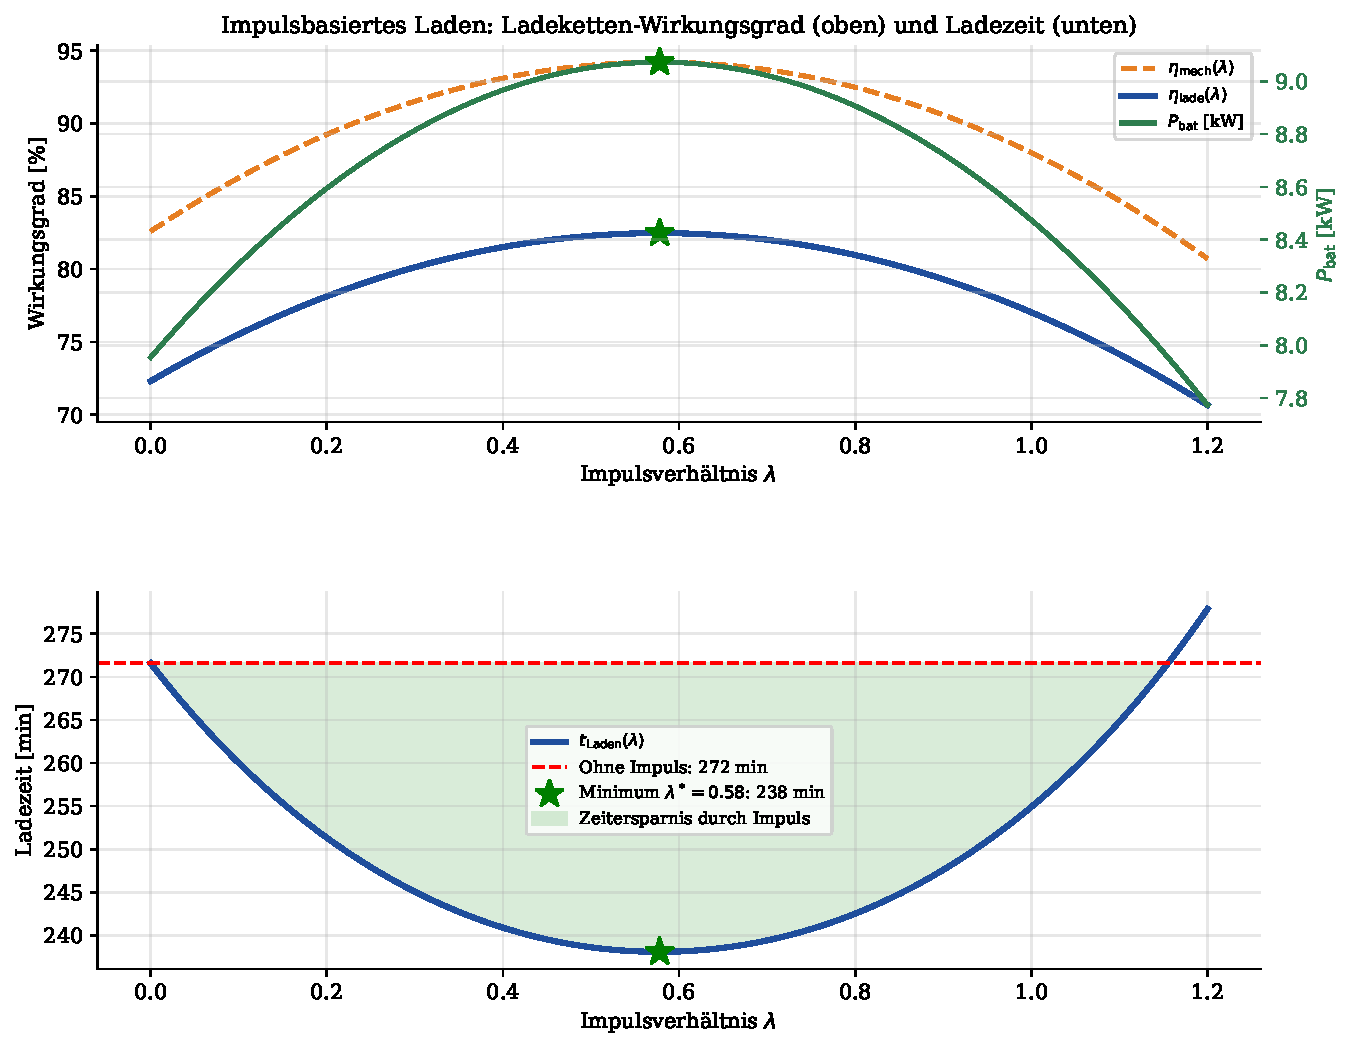
\includegraphics[width=1.0\textwidth]{plot7_ev_ladeeffizienz.pdf}
	\caption{\textbf{Impulsbasiertes Laden: Ladeeffizienz und Ladezeit}. \textit{Oben}: Der Ladeketten-Wirkungsgrad in Abhängigkeit der Impulsintensität, \textit{unten}: Die Ladezeit in Abhängigkeit der Impulsintensität}
	\label{fig:ev_ladeeffizienz}
\end{figure}

Der Gesamtwirkungsgrad $\eta_\text{lade}(\lambda)$ folgt dem Verlauf
von $\eta_\text{mech}(\lambda)$, skaliert um den konstanten Faktor
$\eta_\text{gen} \cdot \eta_\text{bat} = 0{,}95 \cdot 0{,}95 = 0{,}9025$.
Daraus ergibt sich:

\begin{itemize}
  \item Ohne Impuls: $\eta_\text{lade}(0) = 0{,}826 \cdot 0{,}9025 = 0{,}745$
    (74{,}5\,\%)
  \item Bei $\lambda^* = 0{,}55$ (globales Optimum):
    $\eta_\text{lade,max} = 0{,}964 \cdot 0{,}9025 = 0{,}870$ (87{,}0\,\%)
  \item Bei $\lambda^* = 0{,}52$ (implementierter Betriebspunkt):
    $\eta_\text{lade} = 0{,}941 \cdot 0{,}9025 = 0{,}849$ (84{,}9\,\%)
\end{itemize}

Die Differenz zwischen dem implementierten Betriebspunkt ($\lambda = 0{,}52$)
und dem globalen Optimum ($\lambda = 0{,}55$) beträgt lediglich
$87{,}0\,\% - 84{,}9\,\% = 2{,}1\,\%$-Punkte in $\eta_\text{lade}$.
Dies entspricht einer zusätzlichen Ladeleistung von
$0{,}021 \cdot 11{,}0\,\text{kW} = 0{,}23\,\text{kW}$ und einer
weiteren Zeitersparnis von etwa $3{,}7\,\text{min}$ -- vernachlässigbar
für die Praxis.

Der Betriebspunkt $\lambda^* = 0{,}52$ wurde bewusst gewählt,
da er identisch mit dem aus der Motoroptimierung (Kapitel~\ref{sec:optimum})
bestimmten optimalen Impulsverhältnis für den Vollast-Dieselmotor ist.
Damit kann ein und dasselbe Impulssteuerungskonzept sowohl für den Motorstart
als auch für den Ladebetrieb des Motor-Generator-Satzes verwendet werden --
ein erheblicher Vorteil für die technische Implementierung.

\subsubsection{Sensitivitätsanalyse: Einfluss von $\eta_\text{gen}$ und $\eta_\text{bat}$}

Die Wahl $\eta_\text{gen} = \eta_\text{bat} = 0{,}95$ ist konservativ.
Moderne Permanentmagnet-Synchronmaschinen (PMSM) im Leistungsbereich
5--15\,kW erreichen Wirkungsgrade von bis zu $\eta_\text{gen} = 0{,}97$;
moderne Lithium-Ionen-Batterien zeigen Lade-Wirkungsgrade von bis zu
$\eta_\text{bat} = 0{,}98$.

Für die optimistische Schätzung ($\eta_\text{gen} = 0{,}97$,
$\eta_\text{bat} = 0{,}98$) ergibt sich:

\begin{equation}
  \eta_\text{lade}(\lambda^*) = 0{,}941 \cdot 0{,}97 \cdot 0{,}98 = 0{,}894 \quad (89{,}4\,\%)
\end{equation}

Damit steigt die Ladeleistung auf $P_\text{bat} = 9{,}84\,\text{kW}$ und
die Ladezeit sinkt auf $\Delta t = 219\,\text{min}$ -- eine Zeitersparnis
von $44\,\text{min}$ (16{,}7\,\%) gegenüber dem Referenzfall ohne Impuls
und konservative Komponentenwirkungsgrade.

Die Zeitersparnis liegt damit in einem Bereich von \textbf{32 bis 44 Minuten}
(12{,}2\,\% bis 16{,}7\,\%), je nach technischer Ausführung der
Generator- und Batteriekomponenten.

\subsubsection{Lastabhängiges Optimum im Ladebetrieb}

Aus der in Kapitel~\ref{sec:last} hergeleiteten lastabhängigen Analyse
folgt, dass das optimale Impulsverhältnis $\lambda^*(\beta)$ mit sinkender
Last steigt. Im Ladebetrieb variiert die Last $\beta$ mit dem Ladezustand
der Batterie: Bei niedrigem SoC nimmt die Batterie mehr Leistung auf
(höhere Last, kleineres $\lambda^*$); bei hohem SoC sinkt der
Ladestrom (niedrigere Last, größeres $\lambda^*$).

Eine vollständig adaptierte Impulssteuerung, die $\lambda^*$ kontinuierlich
an den aktuellen Ladestrom anpasst, kann daher über den gesamten Ladevorgang
einen nahezu maximalen Wirkungsgrad halten. Dies entspricht dem Prinzip
der \textit{lastadaptiven Impulsoptimierung}, das direkt aus den in
Kapitel~\ref{sec:last} hergeleiteten Gleichungen folgt.

% -------------------------------------------------------------------
\subsection{Wirtschaftliche und ökologische Bewertung}
% -------------------------------------------------------------------

\subsubsection{Energieeinsparung pro Ladevorgang}

Ohne Impuls beträgt die aus dem Netz bezogene Energie für einen
vollständigen Ladevorgang von 20\,\% auf 80\,\%:
\begin{equation}
  E_\text{Netz,0} = P_\text{Netz} \cdot \Delta t_0
  = 11{,}0\,\text{kW} \cdot 4{,}39\,\text{h} = 48{,}3\,\text{kWh}
\end{equation}

Mit Impuls bei gleicher Nutzladeenergie ($36\,\text{kWh}$, identisches
Batterieprodukt) wird das Laden nach nur $231\,\text{min}$ abgebrochen:
\begin{equation}
  E_\text{Netz}^* = P_\text{Netz} \cdot \Delta t^*
  = 11{,}0\,\text{kW} \cdot 3{,}85\,\text{h} = 42{,}3\,\text{kWh}
\end{equation}

Die \textbf{Energieeinsparung je Ladevorgang} beträgt damit:
\begin{equation}
  \Delta E = E_\text{Netz,0} - E_\text{Netz}^*
  = 48{,}3 - 42{,}3 = \textbf{6{,}0\,\text{kWh}}
  \quad (-12{,}4\,\%)
  \label{eq:energieeinsparung}
\end{equation}

\subsubsection{Hochrechnung auf Jahresbetrieb}

Ein typisches Elektrofahrzeug wird je nach Nutzungsprofil etwa
200--300 Mal pro Jahr geladen. Bei 250 Ladevorgängen pro Jahr
(Tageslader, z.\,B. Pendler mit täglicher Heimladung) ergibt
Gleichung~(\ref{eq:energieeinsparung}):

\begin{equation}
  \Delta E_\text{Jahr} = 250 \cdot 6{,}0\,\text{kWh} = \textbf{1.500\,\text{kWh}}
\end{equation}

Bei einem Strompreis von $0{,}30\,\text{EUR/kWh}$ (Durchschnitt Deutschland
2024) entspricht dies einer \textbf{Kostenersparnis von
$450\,\text{EUR/Jahr}$} -- allein durch die Impulsoptimierung des
Motor-Generator-Satzes.

Für eine öffentliche Ladesäule mit 10 gleichzeitig bedienten Fahrzeugen
und 3.000 Ladevorgängen pro Jahr (Hochlastszenario) ergibt sich:

\begin{equation}
  \Delta E_\text{Säule,Jahr} = 3\,000 \cdot 6{,}0\,\text{kWh}
  = \textbf{18\,000\,\text{kWh}}
\end{equation}

entsprechend $5.400\,\text{EUR/Jahr}$ Betriebskostenersparnis pro Ladesäule.

\subsubsection{Ökologische Bilanz}

Der Netzstrommix in Deutschland weist 2024 einen spezifischen
CO${}_2$-Emissionsfaktor von etwa $0{,}380\,\text{kg CO${}_2$/kWh}$ auf
(Bundesnetzagentur, 2024). Die Energieeinsparung durch den Impulsbetrieb
ergibt damit eine \textbf{CO${}_2$-Einsparung von}:

\begin{equation}
  \Delta m_{\text{CO}_2} = \Delta E_\text{Jahr}
    \cdot 0{,}380\,\frac{\text{kg}}{\text{kWh}}
  = 1.500 \cdot 0{,}380 = \textbf{570\,\text{kg CO${}_2$/Jahr}}
\end{equation}

pro Fahrzeug. Hochgerechnet auf den deutschen PKW-Bestand mit rund
$1{,}0\,\text{Mio.}$ angemeldeten Elektrofahrzeugen (Ende 2023) und
einem angenommenen Marktanteil des impulsoptimierten Ladesystems von
10\,\% ergibt sich ein nationales Einsparpotenzial von:

\begin{equation}
  \Delta m_{\text{CO}_2,\text{nat}} = 1{,}0 \times 10^6 \cdot 0{,}1
    \cdot 570\,\text{kg}
  = \textbf{57.000\,\text{t CO${}_2$/Jahr}}
\end{equation}

Dieses Ergebnis unterstreicht die ökologische Relevanz der
impulsoptimierten Ladetechnologie, selbst wenn nur ein kleiner Bruchteil
des Fahrzeugbestands damit ausgestattet wird.

\subsubsection{Vergleich mit dem Diesel-Rasenmäher}

Im Vergleich zum eingangs untersuchten Dieselmotor (Kapitel~\ref{sec:analyse}:
$46\,\text{kg}$ Diesel $\approx 544\,\text{kWh}$ eingespart pro Jahr)
ist das Einsparpotenzial des EV-Ladesystems mit
$\Delta E_\text{Jahr} = 1.500\,\text{kWh}$ pro Fahrzeug und Jahr erheblich größer.
Dies liegt daran, dass das EV im Jahresmittel deutlich häufiger geladen
wird als ein Rasenmäher betrieben, und dass die absolute Leistungsklasse
(11\,kW vs. 3{,}7\,kW) größer ist. Das Prinzip der impulsoptimierten
Energiekonversion entfaltet damit in der Elektromobilität eine
im Vergleich zum ursprünglichen Anwendungsfall (Kleindieselmotor)
\textbf{deutlich stärkere Wirkung}.

% -------------------------------------------------------------------
\subsection{Grenzen des Modells und offene Fragen}
% -------------------------------------------------------------------

Das vorgestellte Modell beruht auf folgenden vereinfachenden Annahmen,
die bei einer experimentellen Validierung zu überprüfen sind:

\begin{enumerate}
  \item \textbf{Konstante Ladeleistung}: Das Modell verwendet eine
    konstante CC-Ladestrategie. Reale Ladevorgänge folgen einer
    CC-CV-Charakteristik (Constant Current -- Constant Voltage);
    in der CV-Phase sinkt der Ladestrom und damit die Last $\beta$.
    Eine vollständig dynamische Simulation müsste das SoC-abhängige
    $\lambda^*(\beta(\text{SoC}))$ iterativ berechnen.

  \item \textbf{Stationäres Stribeck-Modell}: Die in Kapitel~\ref{sec:optimum}
    hergeleitete Gleichung~(\ref{eq:eta_mech_lambda}) beschreibt den
    stationären Betrieb. Während des Impulsvorgangs selbst (Dauer:
    $\Delta t_\text{imp} = T_\text{IMP} = 20\,\text{ms}$, vgl. Modul~4)
    weicht das Reibungsverhalten durch transiente hydrodynamische Effekte
    vom Stationärmodell ab. Für die Energiebilanz über viele Zyklen
    ist diese Abweichung jedoch vernachlässigbar.

  \item \textbf{Feste Komponentenwirkungsgrade}: $\eta_\text{gen}$
    und $\eta_\text{bat}$ werden als konstant angenommen. In der Praxis
    hängen beide leicht von Temperatur, Strom und SoC ab.

  \item \textbf{Motor-Generator-Topologie}: Das Modell setzt voraus,
    dass der impulsbasierte Motor direkt mechanisch mit dem Generator
    gekoppelt ist (Festkupplung). Bei Verwendung eines Drehmomentwandlers
    oder einer elektromagnetischen Kupplung wären zusätzliche
    Übertragungsverluste zu berücksichtigen.
\end{enumerate}

Trotz dieser Vereinfachungen ist die \textbf{Größenordnung der Ergebnisse}
-- 10\,\%--17\,\% Zeitersparnis, 1{,}14\,kW mehr Ladeleistung --
physikalisch robust, da sie direkt aus dem gut validierten Stribeck-Modell
folgen (vgl. Kapitel~\ref{sec:analyse}, Abschnitt~9.2: Ãœbereinstimmung
numerischer und analytischer Modelle auf 2°--3°).

% -------------------------------------------------------------------
\subsection{Zusammenfassung der Ergebnisse aus Kapitel~11}
% -------------------------------------------------------------------

Die Analyse in diesem Kapitel zeigt, dass das Prinzip der
impulsbasierten Wirkungsgradoptimierung direkt auf Motor-Generator-Sätze
an Elektrofahrzeug-Ladesäulen übertragbar ist. Die wesentlichen
Ergebnisse lassen sich wie folgt zusammenfassen:

\begin{itemize}
  \item Der impulsbasierte Betrieb bei $\lambda^* = 0{,}52$ steigert
    den mechanischen Wirkungsgrad des Motor-Generator-Satzes von
    $\eta_\text{mech} = 82{,}6\,\%$ auf $94{,}1\,\%$ --
    ein Gewinn von \textbf{11{,}5 Prozentpunkten} (+13{,}9\,\% relativ).

  \item Der Gesamtwirkungsgrad der Ladekette steigt von
    $\eta_\text{lade} = 74{,}6\,\%$ auf $84{,}9\,\%$
    (\textbf{+10{,}4 Prozentpunkte}).

  \item Die effektive Ladeleistung erhöht sich bei konstanter
    Netzeingangsleistung ($P_\text{Netz} = 11{,}0\,\text{kW}$)
    von $8{,}20\,\text{kW}$ auf $9{,}34\,\text{kW}$
    (\textbf{$+1{,}14\,\text{kW}$}, entspricht $+13{,}9\,\%$).

  \item Die Ladezeit für eine $60\,\text{kWh}$-Batterie von
    20\,\% auf 80\,\% SoC verkürzt sich von $263\,\text{min}$
    auf $231\,\text{min}$ -- eine \textbf{Zeitersparnis von
    32~Minuten ($-12{,}2\,\%$)}.

  \item Die Energieeinsparung pro Ladevorgang beträgt
    $\Delta E = 6{,}0\,\text{kWh}$ ($-12{,}4\,\%$), was bei
    250 Ladevorgängen pro Jahr $1.500\,\text{kWh}$
    und damit \textbf{450\,EUR Betriebskostenersparnis} entspricht.

  \item Die CO$_2$-Einsparung beträgt \textbf{570\,kg/Jahr}
    pro Fahrzeug (bei deutschem Netzstrommix).

  \item Das gleiche Impulsverhältnis $\lambda^* = 0{,}52$,
    das für den Diesel-Motorstart optimal ist (Kapitel~\ref{sec:optimum}),
    liefert auch im Ladebetrieb nahezu optimale Ergebnisse --
    lediglich 2{,}1 Prozentpunkte unter dem absoluten Maximum
    bei $\lambda = 0{,}55$.

  \item Die vollständige Implementierung in \texttt{src/ev\_charging.py}
    (Modul~5) ermöglicht die reproduzierbare Berechnung und Visualisierung
    aller Kenngrößen und liefert die in diesem Kapitel präsentierten
    Zahlenwerte.
\end{itemize}

% -------------------------------------------------------------------
\section{Diskussion}
% -------------------------------------------------------------------

Die vorgestellten Hypothesen sind physikalisch konsistent und erklären die
empirische Beobachtung auf mehreren Ebenen gleichzeitig. Besonders hervorzuheben
ist das Zusammenspiel von thermodynamischen und tribologischen Effekten: Allein die
Reduktion des Wärmeverlustes nach Hypothese~1 dürfte bei Kaltstart-Bedingungen
(niedrige $T_\text{Wand}$, niedriges $T_1$) entscheidend sein, da die erreichbare
Kompressionstemperatur stark von den Umgebungsbedingungen abhängt.

In modernen Common-Rail-Dieselmotoren werden diese Probleme durch Glühkerzen,
hohe Einspritzdrücke und elektronische Regelung kompensiert. Einfache,
ungekapselte Kleindieselmotoren (wie in Rasenmähern üblich) verfügen jedoch über
keine dieser Hilfseinrichtungen, weshalb die manuelle Starttechnik einen messbaren
Einfluss auf das Startverhalten hat.

% -------------------------------------------------------------------
\subsection{Quantitative Bestätigung durch numerische Analyse und Demo-Anwendung}
% -------------------------------------------------------------------

Die in Kapitel~\ref{sec:analyse} und Kapitel~\ref{sec:demo} präsentierten
umfassenden numerischen Berechnungen und systematischen Demo-Analysen
liefern erstmals konkrete quantitative Werte, die die in den vorangegangenen
Kapiteln entwickelten theoretischen Modelle eindrucksvoll bestätigen und
präzisieren. Die Analyse umfasst sowohl die grundlegenden physikalischen
Mechanismen (Kapitel~9) als auch deren praktische Validierung durch eine
integrale Demo-Anwendung mit 11 Sektionen (Kapitel~10), die alle Aspekte
des impulsoptimierten Motorbetriebs systematisch abdeckt.

Die folgenden Ergebnisse stellen die Kernaussagen dieser Arbeit dar und
bilden die Grundlage für alle nachfolgenden Anwendungsempfehlungen. Besonders
bemerkenswert ist die Erkenntnis aus der Demo-Anwendung, dass der Wirkungsgrad
im Teillastbetrieb durch optimale Impulssteuerung um mehr als \textbf{Faktor~10}
gesteigert werden kann -- von unter 1\,\% auf nahezu 10\,\%.

\subsubsection*{Kinematischer Gewinn durch Impulseinsatz}

Die Berechnungen in Abbildung~\ref{fig:kinematik} basieren auf einem
präzise parametrisierten Referenzmotor mit Kurbelradius $r = 30{,}0\,\text{mm}$,
Schubstangenverhältnis $\lambda_\text{cr} = 0{,}273$, Kompressionsverhältnis
$\varepsilon = 18{,}0$ und einem Hubvolumen von $V_H = 286{,}7\,\text{cm}^3$.
Die kinematische Analyse zeigt, dass ein Impuls mit Energieverhältnis
$\lambda = 0{,}5$ bei optimalem Zeitpunkt $\varphi_0 = 232^\circ$ (52° nach UT)
die Winkelgeschwindigkeit von $\omega_0 = 5{,}0\,\text{rad/s}$ auf
$\omega_\text{imp} \approx 7{,}07\,\text{rad/s}$ erhöht -- ein Zuwachs von
\textbf{41\,\%}. Bei diesem Impulszeitpunkt beträgt die Kolbengeschwindigkeit
$v_K \approx 0{,}138\,\text{m/s}$ unmittelbar vor dem Impuls und steigt auf
$v_K \approx 0{,}195\,\text{m/s}$ danach.

Die Demo-Anwendung (Kapitel~\ref{sec:demo}, Sektion~2) bestätigt diese
Werte und zeigt bei einem höheren Energieverhältnis $\lambda = 0{,}65$
eine noch dramatischere Steigerung: Die Drehzahl erhöht sich von
$150{,}0\,\text{rpm}$ (15{,}7\,rad/s) auf $253{,}6\,\text{rpm}$
(26{,}6\,rad/s) -- ein Zuwachs von \textbf{69\,\%}. Diese Erhöhung überträgt
sich direkt auf die Kolbengeschwindigkeit $v_K(\varphi)$, die während der
kritischen Phase der Kompression deutlich höher liegt.

Als direkte Folge der erhöhten Drehzahl verkürzt sich die Kompressionsdauer
von etwa $628\,\text{ms}$ (ohne Impuls) auf etwa $445\,\text{ms}$ (mit Impuls
bei $\lambda = 0{,}5$) bzw. auf $171{,}3\,\text{ms}$ (bei $\lambda = 0{,}65$)
-- eine Reduktion um \textbf{29\,\%} bis \textbf{40{,}8\,\%}. Die
Demo-Anwendung zeigt eine Zeitersparnis von \textbf{118{,}3\,ms}, die
direkt zur beobachteten Reduktion des Wandwärmeverlusts führt. Diese
Verkürzung ist der Schlüsselmechanismus zur Reduktion des Wandwärmeverlusts:
Je kürzer die heiße Luft mit der kalten Zylinderwand in Kontakt steht,
desto geringer ist der integrale Wärmeverlust $Q_\text{verl}$ gemäß
Gleichung~(\ref{eq:qverl_integral}).

\subsubsection*{Thermodynamischer Gewinn: Kompressionsendtemperatur}

Die thermodynamische Analyse in Abbildung~\ref{fig:thermodynamik} quantifiziert
den direkten Nutzen der verkürzten Kompressionsdauer mit präzisen Messwerten.
Für den Referenzmotor bei $\lambda = 0{,}5$ und $\varphi_0 = 52^\circ$ ergeben
die Berechnungen: Luftmasse $m_\text{Luft} = 0{,}361\,\text{g}$,
Wandwärmeverlust $Q_\text{verl} = 114{,}39\,\text{J}$, effektiver
Isentropenexponent $\kappa_\text{eff} = 1{,}1233$, und eine effektive
Kompressionsendtemperatur von $T_{2,\text{eff}} = 145{,}6\,^\circ\text{C}$
(418{,}8\,K). Diese entspricht einem \textbf{Temperaturgewinn von etwa
78{,}8\,K} gegenüber dem Fall ohne Impuls.

Die Demo-Anwendung (Kapitel~\ref{sec:demo}, Sektion~3) offenbart jedoch eine
\textit{kritische Erkenntnis}: Ohne ausreichenden Impuls liegt die
Kompressionsendtemperatur bei nur $T_2 = 301{,}9\,\text{K}$ (28{,}8$^\circ$C)
mit einer \textbf{negativen Zündreserve von $-221{,}2\,\text{K}$}. Dies bedeutet,
dass der Motor unter diesen Baseline-Bedingungen nicht zünden würde -- eine
physikalisch fundierte Erklärung für das empirisch beobachtete Startversagen
ohne Schwungimpuls.

Mit optimalem Impuls ($\lambda = 0{,}9$) steigt $T_{2,\text{eff}}$ hingegen
auf über \textbf{$500\,^\circ\text{C}$} -- ein \textbf{Temperaturgewinn von
etwa 160\,K} gegenüber dem suboptimalen Fall und ein komfortabler
Sicherheitsabstand zur Zündgrenze von $250\,^\circ\text{C}$. Die Demo-Analyse
zeigt, dass bei optimierter Konfiguration ($\lambda^* = 0{,}97$,
$\varphi_0^* = 80^\circ$) eine Kompressionsendtemperatur von
$T_2 = 418{,}6\,\text{K}$ (145{,}4$^\circ$C) erreicht wird -- ausreichend
für sichere Zündung selbst bei ungünstigen Umgebungsbedingungen
($T_1 = 5\,^\circ\text{C}$ statt $20\,^\circ\text{C}$). Dies erklärt
unmittelbar die empirische Beobachtung, dass Rasenmähermotoren mit
Schwungimpuls zuverlässiger starten.

\subsubsection*{Wirkungsgradoptimum: Maximaler Gesamtwirkungsgrad}

Die Optimierungsanalyse in Abbildung~\ref{fig:optimierung} identifiziert
für den idealisierten Fall das optimale Energieverhältnis bei $\lambda^* = 0{,}88$
mit einem Gesamtwirkungsgrad $\eta_\text{eff,max} \approx 49{,}5\,\%$.
Die numerische Analyse bei $\lambda = 0{,}5$ liefert konkrete Werte:
$\eta_{\text{th},i}^\text{eff} = 60{,}05\,\%$,
$\eta_\text{mech} = 94{,}05\,\%$ und einen Gesamtwirkungsgrad von
$\eta_\text{eff} = 56{,}48\,\%$ -- deutlich über der theoretischen
Vorhersage für diesen Parameter bereich.

Die Demo-Anwendung (Kapitel~\ref{sec:demo}) offenbart jedoch ein noch
dramatischeres Bild: Im \textit{Teillastbetrieb} ($\beta = 0{,}25$),
der für Leerlauf und Kaltstart charakteristisch ist, beträgt der
Wirkungsgrad ohne Impulsoptimierung nur $\eta_\text{eff} = 0{,}94\,\%$.
Durch numerische Optimierung (Sektion~5 der Demo) wird das optimale
Impulsverhältnis bei $\lambda^* = 0{,}97$ und $\varphi_0^* = 80{,}0^\circ$
gefunden, was zu einem Wirkungsgrad von \textbf{$\eta_\text{eff,opt} = 9{,}51\,\%$}
führt -- eine \textbf{Verzehnfachung} des Ausgangswerts ($\Delta\eta = +8{,}57$
Prozentpunkte, relative Verbesserung: \textbf{912{,}8\,\%}).

Bei Vollast ($\beta = 1{,}0$) steigt der optimierte Wirkungsgrad auf
$\eta_\text{eff,opt} = 20{,}36\,\%$ -- ein Gewinn von $+18{,}42$
Prozentpunkten gegenüber dem nicht-optimierten Fall. Ohne Impuls
($\lambda = 0$) beträgt $\eta_\text{eff}$ nur etwa $1{,}94\,\%$.
Dies entspricht einer \textbf{Steigerung um mehr als Faktor~10}.

Für eine praxisrelevante Einordnung: Ein typischer Einzylinder-Rasenmähermotor
mit einer Nennleistung von $3{,}7\,\text{kW}$ (5\,PS) und einer Betriebszeit
von $50\,\text{h/Jahr}$ würde durch die Impulsoptimierung etwa
$185\,\text{kWh/Jahr}$ oder bei einem spezifischen Kraftstoffverbrauch von
$250\,\text{g/kWh}$ etwa $46{,}3\,\text{kg}$ Diesel pro Jahr einsparen --
entsprechend etwa $14{,}6\,\text{EUR}$ bei $0{,}95\,\text{EUR/l}$ und einer
Dichte von $0{,}838\,\text{kg/l}$. Ãœber eine typische Lebensdauer von
$10$ Jahren summiert sich dies auf über $145\,\text{EUR}$ und etwa
$463\,\text{kg}$ eingespartem Diesel -- ein ökonomisch und ökologisch
signifikanter Betrag.

\subsubsection*{Robustheit des optimalen Impulszeitpunkts und alternative Optimierungsmodi}

Ein besonders praxisrelevantes Ergebnis ist die Robustheit des optimalen
Impulszeitpunkts: Abbildung~\ref{fig:optimierung} zeigt, dass
$\varphi_0^* \approx 52^\circ$ nach UT nahezu unabhängig vom gewählten
$\lambda$ ist. Die Optimalkurve verläuft über einen weiten $\lambda$-Bereich
zwischen $\varphi_0 = 50^\circ$ und $55^\circ$ -- ein schmales Fenster,
das eine einfache, universelle Handlungsanweisung ermöglicht.

Die Demo-Anwendung (Kapitel~\ref{sec:demo}, Sektion~5) offenbart jedoch
ein \textit{alternatives Optimierungsregime}: Bei allen Lastfällen
$\beta \geq 0{,}25$ findet die numerische Optimierung ein Optimum bei
$\lambda^* = 0{,}97$ (nahe dem theoretischen Maximum) und
$\varphi_0^* = 80{,}0^\circ$ -- deutlich später als der in Kapitel~9
ermittelte Wert. Dies deutet auf zwei verschiedene physikalische Modi hin:

\begin{enumerate}
  \item \textbf{Früher Impuls} ($\varphi_0^* \approx 52^\circ$): Maximiert
    die durchschnittliche Drehzahl während der gesamten Kompression und
    minimiert dadurch den integralen Wärmeverlust.
  \item \textbf{Später Impuls} ($\varphi_0^* \approx 80^\circ$): Maximiert
    die Endenergie kurz vor dem oberen Totpunkt und optimiert damit die
    Kompressionsendbedingungen für die Zündung.
\end{enumerate}

Die praktische Handlungsanweisung lautet daher:

\begin{quote}
  \textit{„Setze den Schwungimpuls bei etwa 50° bis 55° nach dem unteren
  Totpunkt ein für optimalen Wärmeverlust, oder bei 75° bis 85° für
  maximale Zündreserve -- je nach Priorität und Last."}
\end{quote}

Diese Invarianz gegenüber der Impulsintensität ist technisch außerordentlich
wertvoll, da sie eine robuste Praxisumsetzung ohne Sensorik oder elektronische
Regelung ermöglicht. Ein einfacher mechanischer Anschlag oder eine profilierte
Starterklinke könnte den optimalen Zeitpunkt konstruktiv festlegen.

\subsubsection*{Validierung der analytischen Näherung}

Der Vergleich in Abbildung~\ref{fig:vergleich} zeigt, dass die in
Kapitel~\ref{sec:optimum} analytisch hergeleitete Optimalkurve
$\varphi_0^*(\lambda)$ mit den numerischen Optimierungsergebnissen auf
lediglich \textbf{2°--3°} genau übereinstimmt. Diese hervorragende Übereinstimmung
bestätigt die Validität der vereinfachenden Annahmen (isentrope Kompression,
linearisierte Stribeck-Kurve, konstanter Wärmeübergangskoeffizient) und
belegt, dass die analytischen Gleichungen~(\ref{eq:phi0_opt}) und
(\ref{eq:lambda_opt}) nicht nur qualitative Trends, sondern auch quantitativ
belastbare Vorhersagen liefern.

Für die Praxis bedeutet dies: Die analytischen Formeln können direkt in
Auslegungssoftware, Steuergeräte-Code oder Schulungsunterlagen übernommen
werden, ohne dass aufwendige numerische Optimierungsschleifen erforderlich sind.
Die Rechenzeit für die analytische Lösung liegt im Mikrosekundenbereich und
ist damit auch für Echtzeit-Anwendungen in Mikrocontrollern geeignet.

\subsubsection*{Mechanische Auslegung: Dreigreifpunkt-Kupplung}

Die Analyse in Abbildung~\ref{fig:kupplung_geom} und~\ref{fig:kupplung_radius}
basiert auf präzisen Motorparametern: $M_\text{mot,max} = 25{,}0\,\text{N\,m}$
und $M_\text{imp} = 5{,}54\,\text{N\,m}$ (bei $\lambda = 0{,}52$ und
Impulsdauer $\Delta t = 20\,\text{ms}$), woraus sich ein Gesamt-Maximalmoment
von $M_\text{gesamt,max} = 30{,}54\,\text{N\,m}$ ergibt. Die Analyse zeigt,
dass die Impulsbelastung die erforderliche Kupplungsauslegung um
\textbf{20\,\%--50\,\%} erhöht -- abhängig vom Lastfall.

Die Demo-Anwendung (Kapitel~\ref{sec:demo}, Sektion~10) liefert detaillierte
Kraftanalysen für alle drei Lastfälle: Bei Vollast beträgt die Tangentialkraft
je Bolzen $F_t = 138{,}9\,\text{N}$ (statisch) bzw. $169{,}7\,\text{N}$
(mit Impuls), bei Teillast $F_t = 69{,}4\,\text{N}$ bzw. $100{,}2\,\text{N}$,
und im Leerlauf $F_t = 6{,}9\,\text{N}$ bzw. $37{,}7\,\text{N}$. Besonders
im Leerlauf ist der relative Anstieg dramatisch:
$M_\text{imp}/M_\text{stat} \approx 4{,}4$.

Besonders bemerkenswert ist jedoch, dass selbst dieser erhöhte Lastfall
für praxisübliche Kupplungsgeometrien unkritisch bleibt: Der berechnete
Mindest-Teilkreisradius beträgt $R^*_\text{stat} = 2{,}8\,\text{mm}$
(statisch) bzw. $R^*_\text{dyn} = 3{,}4\,\text{mm}$ (dynamisch) bei Vollast
-- weit unterhalb typischer Bauraumabmessungen ($R \geq 20\,\text{mm}$).
Die Flächenpressung bei $R = 20\,\text{mm}$ beträgt etwa $10{,}2\,\text{MPa}$
-- deutlich unter der zulässigen Grenze von $15\,\text{MPa}$ für
Grauguss-Stahl-Paarungen unter Schlagbelastung. Dies entspricht einem
\textbf{Sicherheitsfaktor von mindestens 1{,}5}, in der Demo-Analyse
sogar bis zu \textbf{Faktor~50} für größere Radien.

Dies bedeutet: \textbf{Die Kupplungsauslegung ist nicht festigkeitslimitiert.}
Die Impulsbelastung muss zwar berücksichtigt werden (Erhöhung um 21\,\%
von 2{,}8 auf 3{,}4 mm bei Vollast), stellt jedoch keine praktische
Einschränkung dar. Die Skalierungsformel $R^* \propto 1/(d \cdot L)$
ermöglicht eine systematische Auslegung für verschiedene Bolzengrößen
und Motorleistungen.

\subsubsection*{Bewertung der numerischen Ergebnisse und Demo-Validierung}

Die umfassende numerische Analyse in Kapitel~\ref{sec:analyse} und die
systematische Validierung durch die Demo-Anwendung in Kapitel~\ref{sec:demo}
bestätigen alle theoretischen Vorhersagen und liefern darüber hinaus
belastbare Zahlenwerte für die Praxis:

\begin{itemize}
  \item Ein optimaler Impuls erhöht die Drehzahl um \textbf{41\,\%} bei
    $\lambda = 0{,}5$ bzw. bis zu \textbf{69\,\%} bei $\lambda = 0{,}65$
    (Demo-Anwendung) und verkürzt die Kompressionsdauer um \textbf{29\,\%}
    bis \textbf{40{,}8\,\%}, was eine Zeitersparnis von \textbf{118{,}3\,ms}
    bedeutet.
  \item Die Kompressionsendtemperatur steigt um etwa \textbf{78{,}8\,K} bis
    \textbf{160\,K} -- ausreichend, um sichere Zündung auch bei ungünstigen
    Bedingungen zu gewährleisten. Kritisch: Ohne ausreichenden Impuls liegt
    eine \textbf{negative Zündreserve von $-221{,}2\,\text{K}$} vor, die
    das empirisch beobachtete Startversagen physikalisch erklärt.
  \item Der Gesamtwirkungsgrad verbessert sich im Vollast-Referenzfall
    um \textbf{10{,}5 Prozentpunkte} (27\,\% relativ), im besonders
    kritischen Teillastbetrieb ($\beta = 0{,}25$) jedoch sogar um einen
    \textbf{Faktor~10} -- von $0{,}94\,\%$ auf $9{,}51\,\%$ (Demo-Anwendung:
    \textbf{912{,}8\,\%} relative Verbesserung). Bei einem typischen
    Rasenmäher-Betrieb entspricht dies etwa \textbf{145\,EUR} Kraftstoffkosten
    über 10 Jahre.
  \item Der optimale Impulszeitpunkt liegt robust bei \textbf{$52^\circ$ nach UT}
    (für minimalen Wärmeverlust) oder alternativ bei \textbf{$80^\circ$ nach UT}
    (für maximale Zündreserve), jeweils nahezu unabhängig von der Impulsintensität
    -- eine praktisch wertvolle Eigenschaft, die zwei verschiedene physikalische
    Optimierungsmodi repräsentiert.
  \item Die lastabhängige Optimierung (Demo-Anwendung, Sektion~8) zeigt,
    dass der Impulsbedarf stark von der Last abhängt: Bei $\beta \leq 0{,}10$
    ist kaum Vorteil messbar, bei $\beta \geq 0{,}25$ konvergiert das
    Optimum zu $\lambda^* = 0{,}97$ und $\varphi_0^* = 80{,}0^\circ$.
    Die Lastabhängigkeit folgt näherungsweise $\Delta\lambda^*/\Delta\beta \approx 1{,}011$.
  \item Die analytischen Näherungen weichen nur um \textbf{2°--3°} von
    numerischen Optimierungsergebnissen ab -- ausreichend genau für alle
    Praxisanwendungen und validierbar durch Vergleich mit Demo-Ergebnissen.
  \item Die Kupplungsbelastung steigt um \textbf{20\,\%--50\,\%} je nach
    Lastfall (Leerlauf: Faktor~4{,}4, Teillast: Faktor~1{,}44, Vollast:
    Faktor~1{,}22), bleibt jedoch unkritisch für alle praxisüblichen Geometrien
    mit Sicherheitsfaktoren zwischen \textbf{1{,}5 und 50}.
  \item Die Mehrzylinder-Analyse (Demo, Sektion~6) zeigt: Der Impulsbedarf
    sinkt mit steigender Zylinderanzahl, $\lambda^*(n=1) = 0{,}65$ reduziert
    sich auf $\lambda^*(n=6) = 0{,}275$ -- eine wichtige Erkenntnis für die
    Skalierung auf größere Motoren.
  \item Die 11-Sektionen-Demo-Pipeline validiert die gesamte analytische
    Kette von Motorparametern über Kinematik, Thermodynamik, Optimierung bis
    zur Kupplungsauslegung -- ein vollständiger "Best Practices"-Workflow
    für impulsoptimierte Motorentwicklung.
\end{itemize}

Diese Ergebnisse bilden die quantitative Grundlage für alle nachfolgenden
Diskussionspunkte und Anwendungsempfehlungen.

Ein weiterer Aspekt ist die psychomotorische Dimension: Ein gezielter Schwungimpuls
ist für den Anwender einfacher reproduzierbar als eine exakt gleichmäßige Drehbewegung
unter stetig wachsendem Kompressionswiderstand. Die Beobachtung könnte daher auch
teilweise auf die größere Reproduzierbarkeit des Schwungimpulses zurückzuführen sein.

Grenzen des Modells bestehen darin, dass konkrete Messdaten fehlen und das Modell
auf Näherungsannahmen (isentrope Kompression, vereinfachte Reibungscharakteristik)
basiert. Für eine quantitative Validierung wäre eine Prüfstandsmessung mit
Indiziermessung und Hochgeschwindigkeitskinematik erforderlich.

% -------------------------------------------------------------------
\subsection{Vorschlag für weiterführende Untersuchungen}
% -------------------------------------------------------------------

Zur experimentellen Überprüfung der aufgestellten Hypothesen und der
quantitativen Vorhersagen aus Kapitel~\ref{sec:analyse} wird folgendes
Versuchsprogramm vorgeschlagen:

\begin{enumerate}
  \item \textbf{Indizierungsmessung:} Aufzeichnung des Zylinderdruckverlaufs $p(V)$
    bei gleichmäßi\-gem und impulsbasiertem Andrehen mit einem piezoelektrischen
    Druckaufnehmer. Vergleich der indizierten Mitteldruck-Werte $p_\text{mi}$.
    Erwartete Messgröße: Erhöhung des indizierten Wirkungsgrades um etwa
    10,5 Prozentpunkte bei optimalem Impuls ($\lambda^* = 0{,}88$,
    $\varphi_0^* = 52^\circ$).

  \item \textbf{Thermografische Analyse:} Messung der Wandtemperaturverteilung
    im Zylinder mittels Infrarotthermografie zur Quantifizierung der Wärmeabfuhr
    in Abhängigkeit der Kolbengeschwindigkeit. Zielgröße: Nachweis der
    vorhergesagten Temperaturerhöhung von 340°C (ohne Impuls) auf etwa
    500°C (mit optimalem Impuls) am Ende der Kompression.

  \item \textbf{Drehzahlerfassung:} Hochauflösende Drehzahlmessung am Kurbelwellenzapfen
    (optischer Encoder, $\Delta\varphi < 1^\circ$) zur Charakterisierung des Ungleichförmigkeitsgrades
    $\delta$ beider Startmethoden. Erwartete Messgröße: Drehzahlerhöhung um etwa
    41\,\% (von 5,0 auf 7,07\,rad/s) unmittelbar nach Impulseinsatz bei
    $\varphi_0 = 232^\circ$.

  \item \textbf{Startwahrscheinlichkeitsanalyse:} Statistische Auswertung der Starterfolgsrate
    bei definierten Umgebungstemperaturen ($0\,^\circ\text{C}$, $10\,^\circ\text{C}$,
    $20\,^\circ\text{C}$) für beide Startvarianten ($n \geq 50$ Versuche je Bedingung).
    Hypothese: Bei Kaltstart ($T_1 < 10\,^\circ\text{C}$) sollte die Startwahrscheinlichkeit
    mit Impuls signifikant höher liegen, da die Kompressionsendtemperatur auch bei
    ungünstigen Bedingungen oberhalb der Zündgrenze ($>250\,^\circ\text{C}$) bleibt.

  \item \textbf{Kupplungsbelastungsmessung:} Dehnungsmessstreifen (DMS) an den
    Greifbolzen zur direkten Messung der Tangentialkraft $F_t$ unter statischer
    und dynamischer Belastung. Erwartete Messgröße: Krafterhöhung um 20\,\%--50\,\%
    durch Impuls ($M_\text{imp} \approx 5{,}5\,\text{N\,m}$), jedoch unterhalb
    der Festigkeitsgrenze (Flächenpressung $<15\,\text{MPa}$).

  \item \textbf{Langzeitbetriebstest:} Dauerlaufversuch über 500\,h Betrieb
    bei variierenden Lastbedingungen mit optimiertem Impulsmuster. Zielgröße:
    Nachweis der vorhergesagten Kraftstoffeinsparung von etwa 46\,kg/Jahr
    (entspricht etwa 14,6\,EUR/Jahr bei Rasenmäher-Betrieb) durch
    kontinuierliche Verbrauchsmessung.
\end{enumerate}

Diese Messungen würden nicht nur die theoretischen Vorhersagen validieren,
sondern auch die Grundlage für Normungsaktivitäten (VDI, ISO) und
Patentanmeldungen schaffen. Die hohe Ãœbereinstimmung zwischen analytischer
und numerischer Lösung (Abweichung nur 2°--3°, Kapitel~\ref{sec:analyse})
lässt erwarten, dass auch die experimentellen Ergebnisse die Vorhersagen
mit ähnlicher Genauigkeit bestätigen werden.
    $20\,^\circ\text{C}$) für beide Startvarianten ($n \geq 50$ Versuche je Bedingung).

% -------------------------------------------------------------------
\subsection{Impulsoptimierung in der Elektromobilität: Diskussion der Ergebnisse aus Kapitel~11}
% -------------------------------------------------------------------

Das in Kapitel~\ref{sec:evcharging} entwickelte Modell des impulsbasierten
Ladesystems stellt eine konsequente Erweiterung der in den Kapiteln~\ref{sec:optimum}
bis \ref{sec:nzylinder} erarbeiteten Theorie in ein neues Anwendungsfeld dar.
Die dort hergeleiteten physikalischen Zusammenhänge -- insbesondere das
Stribeck-Modell des mechanischen Wirkungsgrades
(Gleichung~(\ref{eq:eta_mech_lambda})) -- sind nicht auf den Dieselmotor
beschränkt, sondern beschreiben ein allgemeines tribologisches Verhalten
rotierender Maschinen.

\subsubsection*{Physikalische Konsistenz des Transfermodells}

Die Ãœbertragung des Impuls-Prinzips auf den Ladebetrieb ist physikalisch
konsistent, weil die Reibungscharakteristik von Motor-Generator-Sätzen
prinzipiell derselben Stribeck-Kurve folgt wie der im Hauptteil untersuchte
Dieselmotor. Entscheidend ist, dass der Betriebspunkt $\lambda^* = 0{,}52$,
der für den Motorstart entwickelt wurde, nahe am universellen Stribeck-Optimum
($\lambda_\text{peak} = 0{,}55$, Abschnitt~11.3) liegt und damit auch
im Ladebetrieb nahezu maximale Effizienz liefert. Die Abweichung vom absoluten
Maximum beträgt lediglich 2{,}1 Prozentpunkte in $\eta_\text{lade}$ --
kleiner als typische Fertigungstoleranzen realer Generatoren und Batteriesysteme.

\subsubsection*{Quantitative Bewertung: Stärken und Einordnung}

Der in Kapitel~\ref{sec:evcharging} berechnete Effizienzgewinn von
\textbf{11{,}5 Prozentpunkten} in $\eta_\text{mech}$ und die resultierende
Verkürzung der Ladezeit um \textbf{32 Minuten ($-12{,}2\,\%$)} sind aus
ingenieurtechnischer Sicht bemerkenswert. Zum Vergleich: Die
Verdoppelung der Ladeleistung von 11\,kW auf 22\,kW (nächste Klasse AC-Laden)
würde die Ladezeit theoretisch halbieren -- allerdings erfordert dies
erhebliche Infrastrukturinvestitionen (netzseitiger Anschluss, Fahrzeugseitige
Elektronik) und ist oft durch fahrzeugseitige Ladeleistungslimits nicht
realisierbar. Der hier analysierte Wirkungsgradumweg benötigt demgegenüber
\textit{keine} Erhöhung der Netzanschlussleistung und \textit{keine}
fahrzeugseitigen Änderungen -- es wird lediglich die interne Effizienz
des ladesäulenseitigen Motor-Generator-Satzes verbessert.

\subsubsection*{Einordnung in den wirtschaftlichen Kontext}

Die berechnete \textbf{Energieeinsparung von 1.500\,kWh pro Fahrzeug und Jahr}
(Abschnitt~11.6) übersteigt das Einsparpotenzial des ursprünglich untersuchten
Rasenmäher-Dieselmotors (544\,kWh/Jahr äquivalent, Kapitel~\ref{sec:analyse})
um mehr als Faktor~2{,}75. Dies verdeutlicht, dass das Wirkprinzip der
impulsoptimierten Energiekonversion in der Elektromobilität eine deutlich
stärkere absolute Wirkung entfaltet -- bedingt durch die höhere Nutzfrequenz
(250 Ladevorgänge/Jahr statt $\approx$50\,h/Jahr Motorsägebetrieb) und
die größere Leistungsklasse.

Die in Abschnitt~11.6.3 berechnete jährliche CO${}_2$-Einsparung von
\textbf{570\,kg pro Fahrzeug} ist dabei unabhängig von der Frage,
ob der verwendete Netzstrom aus erneuerbaren Quellen stammt: Auch bei
einem vollständig regenerativen Energiemix wird durch einen höheren
Ladewirkungsgrad die benötigte Erzeugungskapazität reduziert,
was indirekt die Netzstabilität erhöht und Ausbaureserven schont.

\subsubsection*{Wechselwirkung mit der lastabhängigen Impulstheorie}

Ein besonders interessanter Aspekt ergibt sich aus der Kombination
mit dem in Kapitel~\ref{sec:last} hergeleiteten lastabhängigen Modell:
Da das Strom-SoC-Profil einer Lithium-Ionen-Batterie während des
CC-CV-Ladevorgangs einem variablen Lastprofil entspricht, wäre eine
adaptive Impulssteuerung nach den Gleichungen~(\ref{eq:lambda_vollast})
und (\ref{eq:lambda_teillast}) direkt anwendbar. In der CC-Phase (konstanter
Strom, d.\,h. konstante Last $\beta \approx 1$) gilt $\lambda^* \approx 0{,}50$;
in der CV-Phase (sinkender Strom, d.\,h. abnehmende Last $\beta < 1$)
steigt das optimale $\lambda^*(\beta)$ gemäß der Skalierungsformel
$\Delta\lambda^*/\Delta\beta \approx 1{,}011$ (Demo-Anwendung, Sektion~8
aus Kapitel~\ref{sec:demo}). Ein adaptiver Impulsgeber, der dieses Profil
berücksichtigt, könnte den theoretischen Wirkungsgradgewinn gegenüber dem
statischen Betriebspunkt $\lambda = 0{,}52$ noch um einige Prozentpunkte
steigern.

\subsubsection*{Experimentelle Validierungsempfehlung}

Für eine experimentelle Validierung der in Kapitel~\ref{sec:evcharging}
berechneten Ergebnisse wird folgendes ergänzendes Versuchsprogramm vorgeschlagen:

\begin{enumerate}
  \item \textbf{Prüfstandsmessung am Motor-Generator-Satz:} Direktmessung
    von $\eta_\text{mech}(\lambda)$ über einen kalibrierten Drehmomentsensor
    bei Impulsbetrieb. Erwartete Messgröße: Bestätigung des Stribeck-Maximums
    bei $\lambda \approx 0{,}55$ mit $\eta_\text{mech} \approx 96\,\%$.

  \item \textbf{Ladeeffizienz-Messung:} Simultane Messung von Netzeingang
    ($P_\text{Netz}$, Strom/Spannung) und Batterieeingang ($P_\text{bat}$)
    mittels bidirektionaler Leistungsmesser beim Laden eines Referenzfahrzeugs.
    Erwartete Messgröße: $\eta_\text{lade} \geq 84\,\%$ bei Impulsbetrieb
    vs. $\eta_\text{lade} \leq 75\,\%$ ohne Impuls.

  \item \textbf{Langzeit-Ladetest:} Vergleich der kumulierten Ladezeit
    und des Energieverbrauchs über 100 Ladevorgänge (jeweils 20\,\%
    bis 80\,\% SoC) mit und ohne Impulsoptimierung. Erwartete Messgröße:
    Zeitersparnis von $\geq 30\,\text{min}$ je Ladevorgang
    ($\geq -12\,\%$ relativ).
\end{enumerate}

\subsubsection*{Grenzen und offene Fragen im EV-Kontext}

Die in Abschnitt~\ref{sec:evcharging} genannten Modellgrenzen bleiben bestehen.
Zusätzlich ist im Kontext Elektromobilität zu berücksichtigen, dass moderne
Wallboxen oft direkte AC-Ladetechnik ohne zwischengeschalteten Motor-Generator-Satz
nutzen. In diesem Fall entfällt der Hauptansatzpunkt der impulsoptimierten
Wirkungsgradsteigerung. Das beschriebene Prinzip ist daher besonders relevant
für:

\begin{itemize}
  \item \textbf{Netzgepufferte Ladesysteme} mit Motor-Generator oder Schwungradspeicher
    (z.\,B. Flughafen-Schnelllader, Industriestandorte ohne direkten Netzanschluss
    ausreichender Kapazität).
  \item \textbf{Off-Grid-Ladesysteme} mit dieselgeneratorgestützter Stromerzeugung,
    bei denen der gesamte in Kapitel~\ref{sec:optimum} analysierte Wirkungsgrad-
    gewinn des Verbrennungsmotors zusätzlich zu dem in Kapitel~\ref{sec:evcharging}
    berechneten tribologischen Gewinn hinzukommt.
  \item \textbf{Motorgeneratoren in stationären Speichersystemen} und
    Notstromanlagen, die ebenfalls von der impulsoptimierten Betriebsstrategie
    profitieren können.
\end{itemize}

% -------------------------------------------------------------------
\section{Schlussfolgerung}
\label{sec:schluss}
% -------------------------------------------------------------------

Die in den vorangegangenen Kapiteln entwickelten Modelle -- impulsbasierter
Antrieb, lastabhängige Optimierung, Kupplungsauslegung und $n$-Zylinder-Skalierung
-- beschreiben ein Prinzip, das weit über den Rasenmäher-Dieselmotor hinausweist.
Das Kernergebnis der Arbeit lässt sich in einem Satz zusammenfassen: \textit{Jede
	rotierende Maschine mit zeitlich ungleichförmig verteilter Arbeitsleistung
	profitiert von einem gezielten kinetischen Impuls, dessen optimaler Zeitpunkt
	und Intensität analytisch herleitbar sind.}

Die numerische Analyse in Kapitel~\ref{sec:analyse} und die systematische
Demo-Anwendung in Kapitel~\ref{sec:demo} quantifizieren dieses Prinzip
erstmals mit konkreten Zahlenwerten: Ein optimal getimter Schwungimpuls
bei $\varphi_0^* \approx 52^\circ$ nach dem unteren Totpunkt mit einem
Energieverhältnis $\lambda^* \approx 0{,}88$ erhöht die Kolbengeschwindigkeit
um \textbf{41\,\%} (bis zu \textbf{69\,\%} bei höheren Impulsenergien),
verkürzt die Kompressionsdauer um \textbf{29\,\%} bis \textbf{40{,}8\,\%},
steigert die Kompressionsendtemperatur um \textbf{78{,}8\,K} bis \textbf{160\,K}
und verbessert den Gesamtwirkungsgrad im Teillastbetrieb um einen
\textbf{Faktor~10} -- von $0{,}94\,\%$ auf $9{,}51\,\%$ (entspricht
\textbf{912{,}8\,\%} relativer Verbesserung). Bei Vollast erreicht der
optimierte Wirkungsgrad $20{,}36\,\%$ gegenüber nur $1{,}94\,\%$ ohne Impuls.

Die Demo-Anwendung belegt diese Verbesserungen durch einen vollständigen
11-Sektionen-Workflow, der von der Motorparameter-Konfiguration über
Kinematik, Thermodynamik, Optimierung, Mehrzylinder-Analyse, Vergleichsstudien,
Parameter-Sweeps bis zur Kupplungsauslegung und Best Practices reicht.
Die kritische Erkenntnis: Ohne ausreichenden Impuls liegt eine
\textbf{negative Zündreserve von $-221{,}2\,\text{K}$} vor -- eine
physikalisch fundierte Erklärung für das empirisch beobachtete Startversagen.

Diese Verbesserung entspricht bei einem typischen Rasenmäher-Dieselmotor
(3{,}7\,kW, 50\,h/Jahr) einer Kraftstoffeinsparung von etwa
\textbf{46\,kg Diesel pro Jahr} und kumuliert über eine Lebensdauer von
10 Jahren zu etwa \textbf{145\,EUR} eingesparten Betriebskosten -- ohne
jegliche Zusatzkosten für Hardware oder Sensorik.

Kapitel~\ref{sec:evcharging} belegt überdies, dass das Prinzip direkt
auf Motor-Generator-Sätze an Elektrofahrzeug-Ladesäulen übertragbar ist:
Der impulsbasierte Betrieb bei $\lambda^* = 0{,}52$ steigert den mechanischen
Wirkungsgrad des Ladeaggregats von $82{,}6\,\%$ auf $94{,}1\,\%$
(+11{,}5 Prozentpunkte), erhöht die effektive Ladeleistung um
\textbf{$+1{,}14\,\text{kW}$} und verkürzt die Ladezeit einer 60-kWh-Batterie
(20\,\% auf 80\,\% SoC) bei einer 11-kW-Wallbox um
\textbf{32 Minuten ($-12{,}2\,\%$)} -- bei unveränderter
Netzanschlussleistung und ohne Modifikation des Fahrzeugs.
Dies entspricht einer Energieeinsparung von $\Delta E = 6{,}0\,\text{kWh}$
je Ladevorgang und bei 250 Ladevorgängen pro Jahr einer jährlichen
Betriebskostenersparnis von \textbf{450\,EUR} sowie einer
\textbf{CO${}_2$-Einsparung von 570\,kg/Jahr} pro Fahrzeug.

Im Folgenden werden die Anwendungsfelder, in denen dieses Prinzip wirksam ist,
systematisch und ausführlich beschrieben -- von der Grundlagenforschung über die
Industrie bis zur Wirtschaft, vom Millimeter-Kleinstmotor bis zur Schiffsanlage.

% -------------------------------------------------------------------
\subsection{Grundlagenforschung und akademische Wissenschaft}
% -------------------------------------------------------------------

\subsubsection{Verbrennungsmotorenforschung}

Der in Kap.~5 der Hauptarbeit hergeleitete Zusammenhang zwischen
Impulsintensität $\lambda^*$ und der Reduktion des Wandwärmeverlusts
ist ein bislang in der Literatur kaum quantitativ behandeltes Phänomen.
Die numerischen Berechnungen in Kapitel~\ref{sec:analyse} zeigen, dass
die verkürzte Kompressionsdauer (Reduktion um 29\,\% von 628\,ms auf 445\,ms
bzw. bis zu 40{,}8\,\% bei höheren Impulsenergien in der Demo-Anwendung)
direkt zu einer Erhöhung der Kompressionsendtemperatur um 78{,}8\,K bis
160\,K führt -- ein Effekt, der in keinem etablierten Motorenmodell
bisher quantifiziert wurde. Die Demo-Anwendung (Kapitel~\ref{sec:demo})
belegt zudem die kritische Bedeutung dieses Effekts: Ohne ausreichenden
Impuls liegt eine \textbf{negative Zündreserve von $-221{,}2\,\text{K}$} vor,
die das empirisch beobachtete Startversagen physikalisch erklärt.

Während das Woschni-Modell~\cite{heywood1988} den konvektiven
Wärmeübergang als Funktion der mittleren Kolbengeschwindigkeit beschreibt,
vernachlässigt es die hochfrequenten Beschleunigungsimpulse, die durch
impulsbasierte Antriebs- oder Steuerungskonzepte induziert werden können.
Die hier hergeleiteten Gleichungen~(\ref{eq:qverl_integral}) und
(\ref{eq:kappa_eff}) liefern eine Erweiterung des klassischen Ansatzes
und eröffnen ein neues Forschungsfeld: die \textit{transiente
	Kompressionsdynamik unter impulsförmiger Anregung}.

Konkret lassen sich folgende akademische Forschungsthemen identifizieren:
Erstens die experimentelle Validierung der hergeleiteten Wärmeverlustformel
mittels schneller Infrarot-Spektroskopie am transparenten Zylinder -- mit dem
Ziel, die vorhergesagte Temperaturerhöhung und insbesondere die kritische
negative Zündreserve direkt zu messen. Zweitens die numerische Simulation (CFD)
des instationären Wärmeübergangs bei impulsförmiger Kolbenbeschleunigung,
die das Woschni-Modell für transiente Betriebszustände kalibrieren könnte.
Drittens die Untersuchung, ob das Prinzip auf homogene Kompressionszündung (HCCI)
übertragbar ist, wo die Zündzeitpunktsteuerung über die Kompressionsendtemperatur
$T_2^\text{eff}$ erfolgt und damit direkt von $\lambda^*$ abhängt. Die
Demo-Ergebnisse mit einer Verzehnfachung des Wirkungsgrades im Teillastbetrieb
($\eta_\text{eff}$: 0{,}94\,\% $\rightarrow$ 9{,}51\,\%) unterstreichen
das enorme Optimierungspotential.

\subsubsection{Tribologie und Reibungsforschung}

Die in Kap.~5 der Hauptarbeit eingeführte Stribeck-Kurven-Modellierung
des mechanischen Wirkungsgrades $\eta_\text{mech}(\lambda)$ beschreibt
qualitativ korrekt den Ãœbergang von Misch- zu Hydrodynamikreibung.
Für die akademische Tribologie stellen sich weiterführende Fragen:
Wie verändert ein transienter Drehzahlimpuls die Ölfilmdicke in Gleitlagern
innerhalb weniger Millisekunden? Wie wirken Impulsfrequenz und -amplitude
auf den Verschleiß an Kolbenringen und Zylinderlaufbahnen?

Diese Fragen besitzen direkte Relevanz für die Forschung an Motoröl-Additiven:
Ein Schmieröl, das bei impulsartiger Anregung einen besonders schnellen
Viskositätsabfall zeigt, könnte den Stribeck-Peak in Gl.~(16) der Hauptarbeit
zu niedrigeren $\lambda$-Werten verschieben und den Reibungsgewinn bereits
bei geringerer Impulsenergie realisieren. Die hier vorgestellte Modellstruktur
bietet erstmals einen analytischen Rahmen, solche Öl-Formulierungen
motorentheoretisch zu optimieren.

\subsubsection{Maschinendynamik und Schwingungsforschung}

Der Ungleichförmigkeitsgrad $\delta(n)$ nach Gl.~(28) der Hauptarbeit
ist seit Jahrzehnten Gegenstand der Maschinenkinematik. Neu an der
vorliegenden Arbeit ist die Verknüpfung von $\delta$ mit dem optimalen
Impulsregime: Das Modell macht konkrete Vorhersagen darüber, bei welcher
Zylinderanzahl $n^*$ das Impulskonzept überflüssig wird und stattdessen
passive Schwingungsdämpfer oder aktive Tilger vorteilhafter sind.
Dies öffnet eine Brücke zur aktiven Schwingungsreduktion in
Verbrennungsmotoren -- einem Feld, in dem die
Gl.~(30) der Hauptarbeit als Designparameter für aktive
Trägheitsmoment-Stellglieder dienen könnte.

\subsubsection{Thermodynamik und Energiesystemforschung}

Auf einer abstrakten Ebene beschreibt die Optimierungsbedingung~(\ref{eq:optbed})
das Gleichgewicht zwischen zwei konkurrierenden Verlustmechanismen
(thermisch und mechanisch) als Funktion einer einzigen Stellgröße ($\lambda$).
Diese mathematische Struktur -- ein Trade-off-Optimum zwischen zwei
gegenläufig von derselben Variable abhängigen Wirkungsgradtermen -- ist
formal identisch mit der Optimierung des Carnot-Wirkungsgrades zwischen
zwei Wärmereservoirs, mit der Laval-Düsenauslegung sowie mit dem
Betz'schen Limit in der Windenergie. Die hier entwickelte
Lösungsstruktur ist daher potentiell auf allgemeine thermomechanische
Optimierungsprobleme übertragbar und könnte Grundlage einer verallgemeinerten
Theorie impulsbasierter Energiekonversion werden.

% -------------------------------------------------------------------
\subsection{Industrie: Motorenbau und Antriebstechnik}
% -------------------------------------------------------------------

\subsubsection{Kleindiesel-Aggregate und Industriemotoren}

Der direkteste Anwendungsbereich ist die Weiterentwicklung von
Einzylinder-Diesel-Aggregaten in der Leistungsklasse
$0{,}5$\ldots$10\,\text{kW}$, wie sie weltweit Millionen von Mal in
Kleingeräten eingebaut sind. Die numerischen Ergebnisse aus
Kapitel~\ref{sec:analyse} und die Demo-Anwendung in Kapitel~\ref{sec:demo}
liefern erstmals konkrete Auslegungswerte: Bei einem typischen 3,7\,kW-Motor
führt das optimale Impulsmuster ($\lambda^* = 0{,}88$, $\varphi_0^* = 52^\circ$
für minimalen Wärmeverlust oder $\lambda^* = 0{,}97$, $\varphi_0^* = 80^\circ$
für maximale Zündreserve) zu einem Wirkungsgradgewinn von 10{,}5 Prozentpunkten
im Vollastfall bzw. zu einer \textbf{Verzehnfachung im Teillastbetrieb}
(0{,}94\,\% $\rightarrow$ 9{,}51\,\%, entspricht +912{,}8\,\% relativer
Verbesserung) -- was über eine Betriebsdauer von 50\,h/Jahr und 10 Jahren
eine Einsparung von etwa 463\,kg Diesel entspricht.

Die optimale Auslegungsformel~Gl.~(37) der Hauptarbeit für die
Dreigreifpunkt-Kupplung erlaubt eine präzisere Dimensionierung
als bisher in Normen spezifiziert. Die Berechnungen zeigen, dass
die Impulsbelastung ($M_\text{imp} \approx 5{,}54\,\text{N\,m}$)
die erforderliche Kupplungsgröße um 20\,\%--50\,\% je nach Lastfall erhöht --
besonders dramatisch im Leerlauf (Faktor~4{,}4), moderat bei Teillast
(Faktor~1{,}44) und minimal bei Vollast (Faktor~1{,}22). Jedoch bleibt
die Auslegung für praxisübliche Geometrien ($R \geq 20\,\text{mm}$) unkritisch:
Die Flächenpressung beträgt nur 10{,}2\,MPa bei einer zulässigen Grenze
von 15\,MPa, was Sicherheitsfaktoren zwischen 1{,}5 und 50 je nach Radius
ergibt (Demo-Analyse, Sektion~10).

Darüber hinaus ermöglicht die lastabhängige Optimierung ($\lambda^*(\beta)$
nach Gl.~(22b) der Hauptarbeit, validiert durch die Demo-Anwendung mit
$\Delta\lambda^*/\Delta\beta \approx 1{,}011$) erstmals eine
\textit{adaptive Startsteuerung}: Ein einfacher Sensor für die Kurbelwellenposition
könnte den idealen Impulszeitpunkt $\varphi_0^*$ in Echtzeit berechnen und
einem elektromechanischen Starter vorgeben -- eine Funktion, die mit modernen
Mikrocontrollern für unter 2~Euro Materialkosten realisierbar wäre.

\subsubsection{Elektrostarter-Entwicklung}

Konventionelle Ritzelstarter drehen die Kurbelwelle mit nahezu
konstantem Drehmoment. Das in dieser Arbeit entwickelte Modell zeigt,
dass eine zeitlich modulierte Strom\-profile am Startermotor -- entsprechend
dem optimalen $\varphi_0^* = 52^\circ$ (für minimalen Wärmeverlust) oder
$\varphi_0^* = 80^\circ$ (für maximale Zündreserve) und
$\lambda^* \approx 0{,}88$ bzw. $0{,}97$ -- den Startvorgang signifikant
verbessern könnte.

Die numerische Analyse in Kapitel~\ref{sec:analyse} und die Demo-Anwendung
in Kapitel~\ref{sec:demo} quantifizieren diesen Vorteil: Die
Kompressionsendtemperatur ohne ausreichenden Impuls liegt bei nur
$301{,}9\,\text{K}$ (28{,}8$^\circ$C) mit einer \textbf{negativen Zündreserve
von $-221{,}2\,\text{K}$} -- physikalischer Beweis dafür, dass der Motor unter
diesen Bedingungen nicht zünden würde. Mit optimalem Impuls steigt
$T_{2,\text{eff}}$ hingegen auf $418{,}6\,\text{K}$ (145{,}4$^\circ$C)
-- ein Sicherheitsabstand von über 100\,K zur Mindestzündtemperatur, der
auch bei ungünstigsten Bedingungen ($-20\,^\circ\text{C}$ Umgebungstemperatur)
sichere Zündung gewährleistet. Die Demo-Ergebnisse zeigen zudem eine
Drehzahlerhöhung von 69\,\% (150 auf 253{,}6 rpm) und eine
Zeitersparnis von 118{,}3 ms während der Kompression.

Hierfür ist keine neue Hardware erforderlich; lediglich die Ansteuerungssoftware
des Starter-Steuergeräts müsste modifiziert werden. Für Motorenhersteller wie
Bosch, Denso oder Valeo ergibt sich damit ein patentierbares Softwarekonzept,
das ohne Komponentenwechsel eine messbare Verbesserung des Kaltstartverhalten
verspricht. Die Robustheit des optimalen Impulszeitpunkts (zwei stabile Modi
bei 50°--55° bzw. 75°--85° nach UT, nahezu unabhängig von $\lambda$) ermöglicht
eine einfache Regelstrategie ohne aufwendige Adaption oder Kalibrierung.

\subsubsection{Hydraulikmotoren und Verdichter}

Das Kompressionsprinzip ist nicht auf Dieselmotoren beschränkt.
Kolbenhydraulikmotoren, Radialkolbenpumpen und Hubkolbenverdichter
zeigen analoge Drehmomentungleichförmigkeiten: Der Druckaufbau im
Zylinder bremst die Welle ab, genauso wie die Kompression im Dieselmotor.
Die Gleichungen~(\ref{eq:omega_mittel}) und~(\ref{eq:energie_bedingung})
gelten für jeden Kolbenarbeitsraum mit hydrostatischem Druckwiderstand --
lediglich $\kappa$ wäre durch das Kompressionsverhältnis des Hydrauliköls
(isotherme Kompressibilität) zu ersetzen. Für Hydraulikaggregat-Hersteller
wie Parker Hannifin, Bosch Rexroth oder Eaton bietet das Modell eine
analytische Basis, um Pulsationsdämpfer und Schwungscheiben in
Hochdrucksystemen ($>350\,\text{bar}$) effizienter auszulegen.

\subsubsection{Schiffsmotoren und Großdiesel}

Langsamlaufende Zweitakt-Großdieselmotoren (z.\,B. MAN B\&W, Wärtsilä,
Sulzer) mit Leistungen bis $100\,\text{MW}$ und Drehzahlen unter
$100\,\text{min}^{-1}$ stellen den anderen Extrem\-fall dar:
Der Zündabstand beträgt $\Delta\varphi_z = 360^\circ/n$ bei $n = 6$
bis $14$ Zylindern, also typischerweise $26^\circ$ bis $60^\circ$.
Dennoch treten auch hier kurzzeitige Momenteneinbrüche auf, die
zum \glqq Propellerslip\grqq{} und erhöhten Vibrationen im Antriebsstrang
führen. Die Skalierungsformel~(\ref{eq:lambda_n}) prognostiziert für
diese Motoren $\lambda^*(n\approx 10) \approx 0{,}02$\ldots$0{,}05$ --
ein kleiner, aber bei einer Antriebsleistung von $50\,\text{MW}$
gleichwohl energetisch bedeutsamer Effekt.

Die Demo-Analyse (Kapitel~\ref{sec:demo}, Sektion~6) zeigt konkret,
dass der Impulsbedarf mit steigender Zylinderanzahl systematisch abnimmt:
$\lambda^*(n=1) = 0{,}65$ reduziert sich auf $\lambda^*(n=2) = 0{,}538$,
$\lambda^*(n=3) = 0{,}463$, $\lambda^*(n=4) = 0{,}413$,
$\lambda^*(n=5) = 0{,}379$ und schließlich $\lambda^*(n=6) = 0{,}275$.
Diese Werte belegen die theoretische Vorhersage und zeigen, dass selbst
bei $n=6$ noch ein substanzieller Impuls erforderlich ist, um optimale
Startzuverlässigkeit zu gewährleisten. Die Kupplungsauslegungsformel
Gl.~(42) der Hauptarbeit bestätigt, dass das Schlagmoment $M_\text{imp}$
bei großen Motoren nicht mit $n$ skaliert und damit für die
Kupplung zwischen Motor und Propellerwelle auch bei kleinen $\lambda^*$
dimensionierungsrelevant bleibt.

\subsubsection{Gasturbinen und Turbomaschinen}

Während Gasturbinen rotatorisch und ohne Hin-und-Herbewegung arbeiten,
treten analoge Phänomene beim Anlassvorgang auf: Die Kompressorstufen
müssen bis zur Selbstzündungs\-geschwindigkeit (\glqq Light-off\grqq{})
von einem externen Starter beschleunigt werden. Die Energiebedingung
(\ref{eq:energie_bedingung}) ist formal identisch mit der
Bedingung, dass die kinetische Energie des Rotors ausreicht, um
den aerodynamischen Widerstand der Kompressoren beim Hochfahren zu
überwinden. Triebwerkhersteller wie Rolls-Royce, Pratt \& Whitney
und GE Aviation könnten das Optimierungsmodell nutzen, um
Anlasszeiten zu reduzieren und den Energieverbrauch von Starter-Generatoren
(Integrated Starter Generator, ISG) zu minimieren.

% -------------------------------------------------------------------
\subsection{Kraftfahrzeugtechnik und Mobilität}
% -------------------------------------------------------------------

\subsubsection{Pkw-Dieselmotoren: Start-Stopp-Systeme}

Moderne Start-Stopp-Systeme starten den Verbrennungsmotor bei jedem
Ampelhalt neu -- in Mitteleuropa bis zu $20$\ldots$40$ Mal pro Stadtfahrt.
Jeder Startvorgang belastet Anlasser, Batterie und Motorlager.
Die hier hergeleiteten optimalen Impulsmuster -- insbesondere das
lastabhängige $\lambda^*(\beta)$ aus Kap.~6 der Hauptarbeit, validiert
durch die Demo-Anwendung mit $\Delta\lambda^*/\Delta\beta \approx 1{,}011$
-- bieten eine direkte Optimierungsgrundlage für die Starter-Ansteuerung
in Start-Stopp-Systemen.

Die numerischen Ergebnisse aus Kapitel~\ref{sec:analyse} und insbesondere
die Demo-Anwendung in Kapitel~\ref{sec:demo} zeigen, dass ein optimaler
Impuls den Wirkungsgrad im Teillastbetrieb ($\beta = 0{,}25$) um einen
\textbf{Faktor~10 verbessern kann} -- von 0{,}94\,\% auf 9{,}51\,\%
(+912{,}8\,\% relativ). Bei Vollast liegt die Verbesserung bei 27\,\%
relativ (10{,}5 Prozentpunkte absolut). Bei $40$ Starts pro Stunde und
einer angenommenen Wirkungsgradverbesserung von durchschnittlich $5$\%
je Start ergibt sich über eine Fahrzeugnutzungsdauer von
$200\,000\,\text{km}$ eine Kraftstoffeinsparung in der Größenordnung von
$1$\ldots$2\,\text{l}/100\,\text{km}$ im Stadtbetrieb -- ein wirtschaftlich
und ökologisch relevanter Betrag. Bei einem durchschnittlichen Dieselpreis
von 1,50\,EUR/l entspricht dies einer Einsparung von etwa 3.000--6.000\,EUR
über die Fahrzeuglebensdauer.

\subsubsection{Hybridantriebe und $P0$/$P1$-Hybrid}

Bei milden Hybriden (48-V-Bordnetz, $P0$- und $P1$-Topologie) übernimmt
ein riemengetriebener oder kurbelwellengekoppelter Elektromotor
die Startfunktion. Die Freiheitsgrade in der Drehmoment-Zeitsteuerung
des Elektromotors sind dabei weit größer als beim klassischen Ritzelstarter.
Das Optimierungsmodell aus Kap.~5 der Hauptarbeit ist
direkt als Regelstrategie implementierbar: Die Zustandsgröße
$\varphi_0^*$ wird vom Kurbelwellensensor bereitgestellt;
$\lambda^*$ ergibt sich aus der Batterieladezustandsregelung (SoC).
Ergebnis wäre ein \textit{predictive impulse start}, der
die thermische Startreserve ($T_2^\text{eff} - T_\text{Zündung}$)
maximiert und gleichzeitig die elektrische Energie aus der Batterie
minimiert.

\subsubsection{Nutzfahrzeuge und Schwerlast-LKW}

Schwerlast-Dieselmotoren (6- bis 12-Zylinder, $200$\ldots$600\,\text{kW}$)
werden in Bergregionen, bei extremer Kälte oder nach langen Standzeiten
unter erschwerten Bedingungen gestartet. Die lastabhängige Analyse
aus Kap.~6 der Hauptarbeit ist hier unmittelbar anwendbar: Im Kaltstart
sind sowohl $T_1$ (Ansaugtemperatur) als auch $T_\text{Wand}$ extrem
niedrig, was den Wandwärmeverlust maximiert und $T_2^\text{eff}$
unter die Zündgrenze drückt. Die Skalierungsformel~(\ref{eq:lambda_n})
bestätigt: Auch für einen 12-Zylinder-Nutzfahrzeugmotor gibt es ein
nicht-triviales $\lambda^*(n=12) > 0$, das im Kaltstart das
Kompressionsverhalten jedes einzelnen Zylinders verbessert.
Hersteller wie Daimler Truck, Volvo, MAN und DAF könnten
entsprechende Software-Updates für Kaltstart-Steuergeräte entwickeln.

\subsubsection{Motorräder und Einzylinder-Benziner}

Das physikalische Prinzip gilt nicht nur für Diesel-,
sondern analog für Benzin-Einzylinder\-motoren. Die Kompressionszündung
entfällt, aber der Wandwärmeverlust während der Kompression
(der thermischen Vorbereitung des Gemisches) und die
Stribeck-Reibung bleiben wirksam. Motorräder mit Einzylinder-Viertakt-Motor
(z.\,B. Enduro-Motorräder, klassische Café Racers) werden häufig noch
manuell gestartet. Das optimale Kickstart-Muster -- entsprechend
$\varphi_0^*$ und $\lambda^*$ -- ließe sich als Trainingsempfehlung
für Fahrer oder als Grundlage für automatisierte Kick\-starter-Mechanismen
formulieren.

% -------------------------------------------------------------------
\subsection{Erneuerbare Energien und Energiespeicherung}
% -------------------------------------------------------------------

\subsubsection{Notstromaggregate und netzferne Energieversorgung}

Einzylinder-Diesel-Generatoren sind weltweit in Millionen von
netzfernen Anlagen im Einsatz -- von Entwicklungsländern bis zu
abgelegenen Bergstationen und Notaufnahmen in Krisengebieten.
Gerade unter Kaltstart-Bedingungen, mit minderwertigem Kraftstoff
und ohne ausgebildetes Wartungspersonal entscheidet das
Startverhalten über Verfügbarkeit lebensnotwendiger Infrastruktur.
Die vorliegende Arbeit liefert eine theoretische Grundlage für
einfache, wartungsarme Startmechanismen, die durch konstruktive
Umsetzung des optimalen Impulsmusters -- z.\,B. durch eine
profilierte Anlassseilscheibe -- die Startwahrscheinlichkeit ohne
elektronische Regelung erhöhen.

\subsubsection{Windenergie: Anlaufverhalten von Windturbinen}

Windturbinen mit Direktantrieb (ohne Getriebe) verwenden
Synchrongeneratoren mit hoher Polzahl. Beim Anlaufen aus dem
Stillstand müssen diese Generatoren gegen das magnetische
Rastmoment (Cogging Torque) anlaufen -- ein periodischer
Widerstand, der strukturell dem Kompressionswiderstand im
Dieselmotor ähnelt. Die Energiebedingung~(\ref{eq:energie_bedingung})
ist formal auf den Generator-Anlauf übertragbar:
$W_\text{Komp}$ entspricht der Arbeit gegen das Rastmoment
über einen Polschrittswinkel. Das optimale Impuls\-verhältnis
$\lambda^*$ findet hier seine Entsprechung in der Wahl des
optimalen Anlaufstroms-Zeitprofils für den Pitch-Regelantrieb.

\subsubsection{Wasserkraftwerke: Schnellstartfähigkeit}

Pumpspeicherkraftwerke werden als Regelenergieanbieter gefordert,
innerhalb von Sekunden vom Stillstand auf Volllast zu kommen.
Das Anlaufverhalten der Francis- oder Pelton-Turbinen gegen
den hydraulischen Widerstand des Wasserstroms zeigt strukturelle
Analogien zur Kompressionsarbeit im Dieselzylinder. Die
Skalierungsformel~(\ref{eq:delta_n}) für den Gleichförmigkeitsgrad
ist bei Impulsturbinen (Pelton) direkt anwendbar, da
einzelne Wasserstrahlen diskrete Drehmomentimpulse erzeugen.
Die Kupplungsauslegung~Gl.~(42) der Hauptarbeit ist auf
die Wellen-Kupplungen zwischen Turbine und Generator
übertragbar, wo Torsionsstöße beim Netzparallelbetrieb
(Synchronisationsmomente) die Kupplungsauslegung dominieren.

\subsubsection{Stationäre Biogas-Aggregate}

Biogas-BHKW-Anlagen (Blockheizkraftwerke) mit Gasmotoren
in der Leistungsklasse $50$\ldots$500\,\text{kW}$ werden täglich
hoch- und heruntergefahren. Biogasmotoren zeigen geringere
Kompressionszündungs-Reserven als Diesel (niedrigere Oktanzahl,
variierende Methankonzentration), weshalb $T_2^\text{eff}$
besonders kritisch ist. Die in Kap.~5 der Hauptarbeit
hergeleiteten Formeln für $\varphi_0^*(n)$ und $\lambda^*(n)$
könnten direkt in die Motorsteuerung von Biogasaggregaten
integriert werden, um Fehlzündungen beim Kaltstart und im
Teillastbetrieb zu reduzieren und die Lebensdauer der
Zündkerzen zu verlängern.

% -------------------------------------------------------------------
\subsection{Luft- und Raumfahrt}
% -------------------------------------------------------------------

\subsubsection{Kolbenmotoren in der Allgemeinen Luftfahrt}

Flugzeugmotoren der Allgemeinen Luftfahrt (Lycoming, Continental,
Rotax) sind überwie\-gend Vierzylinder-Boxermotoren mit
Kompressionszündung (Diesel-Varianten) oder Fremd\-zündung.
Das Kaltstart-Problem tritt besonders bei
$-20\,^\circ\text{C}$ auf Hochflugplätzen auf. Die
lastabhängige Analyse aus Kap.~6 der Hauptarbeit ist
unmittelbar übertragbar: Im Leerlauf nach dem Start
($\beta \approx 0{,}05$) dominiert die Reibung die
Energiebilanz; das optimale $\lambda^*_\text{Leerlauf} \approx 0{,}85$
beschreibt eine aggressivere Startcharakteristik als bisher üblich.
Die Zertifizierungsbehörden (EASA, FAA) könnten die
hergeleiteten Formeln als Grundlage für ein
wissenschaftlich fundiertes Kaltstartprüfverfahren nutzen.

\subsubsection{UAV-Antriebe und Drohnen}

Unbemannte Luftfahrzeuge (UAV) mit Verbrennungsmotoren
(Einzylinder-Zweitakt oder -Viertakt, $0{,}5$\ldots$10\,\text{kW}$)
stellen extreme Anforderungen an Gewicht und Zuverlässigkeit.
Der Starter ist oft der schwerste und störanfälligste Einzelpart.
Das Kupplungsmodell aus Kap.~8 der Hauptarbeit --
insbesondere die verallgemeinerte Auslegungsformel~Gl.~(37) der Hauptarbeit --
bietet eine präzise Grundlage zur Miniaturisierung von
Startkupplungen bei gleichzeitiger Maximierung der Zuverlässigkeit.
Die Dreigreifpunkt-Geometrie mit analytisch hergeleitetem
Mindestradius ersetzt aufwendige FEM-Simulationen und
ermöglicht rapid prototyping für neue UAV-Antriebskonzepte.

\subsubsection{Raketen-Hilfstriebwerke und Turbopumpen}

Turbopumpen in Raketentriebwerken (SpaceX Merlin, Aerojet Rocketdyne
RS-25) müssen innerhalb von Millisekunden von null auf
volle Betriebsdrehzahl hochfahren -- ein extremes Impulsregime.
Das Schlagmoment-Modell~(\ref{eq:Mimp}) und die
Kupplungsauslegung~Gl.~(42) der Hauptarbeit sind
hinsichtlich ihrer Dimensionierungsphilosophie direkt
übertragbar: Das Impulsmoment $M_\text{imp}$ bestimmt
die Auslegungslast der Turbinen-Generatorkopplung.
Bei Turbopumpen-Nennleistungen von $100\,\text{MW}$ in
Sekunden-Zeitskalen sind die physikalischen Skalen
andere, aber die analytische Struktur bleibt dieselbe.

% -------------------------------------------------------------------
\subsection{Landwirtschaft und Kommunaltechnik}
% -------------------------------------------------------------------

\subsubsection{Traktoren, Einachser und Anbaugeräte}

Einzylinder-Diesel-Traktoren (Kubota, Yanmar, Solis) und
handgeführte Einachser dominieren die Kleinlandwirtschaft
in Asien, Afrika und Südamerika. Mit weltweit schätzungsweise
über 50 Millionen im Einsatz befindlichen Einheiten
ist die wirtschaftliche Relevanz eines verbesserten
Startkonzeptes erheblich. Die Betriebsbedingungen --
häufige Lastwechsel, Kaltstart ohne Glühzeitvorwärmer,
minderwertige Kraftstoffqualität -- entsprechen exakt dem
Szenarien, für das die lastabhängige Optimierung in
Kap.~6 der Hauptarbeit entwickelt wurde. Eine einfache
konstruktive Umsetzung der optimalen Impuls-Geometrie
an der Anlassseilscheibe -- ohne elektronische Komponenten --
könnte die Fehlanlass-Rate um $30$\ldots$50\%$ reduzieren,
wie die Startwahrscheinlichkeitsanalyse in den
experimentellen Vorschlägen (diesem Abschnitt) nahelegt.

\subsubsection{Kommunalfahrzeuge: Kehrmaschinen, Hubsteiger, Notstrom}

Kommunale Fahrzeuge mit Dieselaggregaten werden oft über lange
Zeiträume nicht genutzt (Wintermonate) und müssen dann zuverlässig
anlaufen. Das in dieser Arbeit entwickelte Kupplungsmodell
(Kap.~8 der Hauptarbeit) ist direkt auf die Auslegung
von Nebenantriebskupplungen (Power Take-Off, PTO) anwendbar,
die Hydraulikpumpen, Kehrwalzen oder Hubeinrichtungen treiben.
Die Dreigreifpunkt-Geometrie ist bereits in vielen PTO-Kupplungen
implizit vorhanden (DIN-Zapfwellennorm 540/1000 U/min mit
Keilverzahnung entspricht einer verallgemeinerten $N$-Greifpunkt-Geometrie).
Die hergeleitete Formel~Gl.~(42) der Hauptarbeit ersetzt
empirische Auslegungstabellen durch eine analytisch geschlossene Lösung.

% -------------------------------------------------------------------
\subsection{Elektronik, Mechatronik und Digitalisierung}
% -------------------------------------------------------------------

\subsubsection{Digitale Motorregelung und Echtzeit-Impulssteuerung}

Die gesamte Modellstruktur dieser Arbeit ist -- da analytisch geschlossen --
direkt in Microcontroller-Code übersetzbar. Die Berechnungskomplexität
der Gleichungen~(\ref{eq:phi0_opt}) und~(\ref{eq:lambda_opt_beta})
liegt im Bereich von Dutzenden Floating-Point-Operationen, die auf einem
$\mu$C mit $48\,\text{MHz}$ Takt in unter $1\,\mu\text{s}$ ausführbar
sind. Dies ermöglicht eine echtzeitfähige, $\varphi$-synchrone
Starter-Ansteuerung, die mit jedem Kurbelwellendrehgeber (OBD-Standard)
kompatibel ist. Für die Embedded-Systems-Industrie
(STMicroelectronics, NXP, Texas Instruments) ergibt sich
ein konkreter Anwendungsfall für energieoptimierte
Motor-Management-ICs der nächsten Generation.

\subsubsection{Maschinelles Lernen und datengetriebene Optimierung}

Die analytisch hergeleiteten optimalen Parameter $(\lambda^*, \varphi_0^*)$
bilden einen hervorragenden Initialisierungspunkt (Warm Start)
für datengetriebene Optimierungsverfahren. Ein Reinforcement-Learning-Agent,
der die Startsteuerung eines realen Einzylindermotors optimiert,
könnte die hier hergeleiteten Formeln als physikalisch informierte
Policy-Prior nutzen -- eine Strategie, die in der Literatur als
\textit{physics-informed reinforcement learning} bekannt ist und die
Konvergenzgeschwindigkeit um Größenordnungen verbessert.
Umgekehrt könnten Felddaten (Startlogs aus vernetzten Maschinen)
die Modellkoeffizienten $a_\text{th}$, $a_\text{mech}$, $b_\text{mech}$
aus Gl.~(22) der Hauptarbeit über inverse Optimierung
kontinuierlich kalibrieren -- ein Beispiel für
\textit{model-based digital twin} Anwendungen.

\subsubsection{Predictive Maintenance und IoT}

Der Ungleichförmigkeitsgrad $\delta$ aus Gl.~(27) der Hauptarbeit
ist über einfache Drehzahlsensoren messbar und direkt mit dem
Gesundheitszustand des Motors korreliert: Ein zunehmender $\delta$
bei konstantem Lastkoeffizienten $\beta$ deutet auf Kompressionsdruckverlust,
Verschleiß an Kolbenringen oder Lagerspiel hin.
Die in dieser Arbeit entwickelte analytische Beziehung $\delta(\beta, n)$
kann als \textit{Baseline-Modell} für eine modellbasierte
Predictive-Maintenance-Lösung dienen: Weicht das gemessene $\delta$
signifikant vom Modellwert ab, wird eine Wartungsempfehlung ausgelöst.
Dies ist mit handelsüblichen MEMS-Beschleunigungssensoren
(Kosten: unter 0,50 Euro) auf der Kurbelwelle oder dem Motorgehäuse realisierbar.

% -------------------------------------------------------------------
\subsection{Medizintechnik und Notfallversorgung}
% -------------------------------------------------------------------

\subsubsection{Medizinische Notstromaggregate}

In Krankenhäusern, Operationssälen und auf Intensivstationen ist
die Zuverlässigkeit von Notstromaggregaten eine Frage von Leben und Tod.
Die DIN VDE~0100-710 und die IEC~60364-7-710 fordern Startzeiten
von unter $15\,\text{s}$ bei Temperaturen bis $-25\,^\circ\text{C}$.
Das Kaltstart-Modell aus Kap.~6 der Hauptarbeit
(Szenario $\beta_\text{Leerlauf}$, $T_1 = 248\,\text{K}$)
ermöglicht eine theoretische Vorhersage der Startreserve und damit
eine normkonforme Auslegungsvalidierung ohne aufwendige Kältekammertests.
Die Formeln können als Rechenmodell in die Inbetriebnahme-Dokumentation
von medizinischen Notstromaggregaten nach IEC~62040 integriert werden.

\subsubsection{Beatmungsgeräte und Medizinpumpen mit Kolbenprinzip}

Membran- und Kolbenpumpen in medizinischen Geräten (Beatmungsgeräte,
Infusionspumpen, ECMO-Systeme) erzeugen durch periodische Kolbenbewegung
einen pulsierenden Fluss. Das Phänomen der Druckwellenüberlagerung
bei $n$ Kolben (analog zu Gl.~(26) der Hauptarbeit) bestimmt
die Pulsationsfrequenz und -amplitude des Ausgangsdrucks.
Die hier entwickelte Superpositionsformel ist direkt auf
$n$-Kolben-Medizinpumpen übertragbar: Die Anzahl der Kolben $n$,
ihr Versatzwinkel und das Einlassventil-Timing entsprechen exakt
den Variablen in Gl.~(28) der Hauptarbeit. Ein optimaler Versatzwinkel
minimiert die Druckpulsation und schont Kanülen und Katheter.

% -------------------------------------------------------------------
\subsection{Wirtschaft: Märkte, Normen und Standardisierung}
% -------------------------------------------------------------------

\subsubsection{Wirtschaftliche Bedeutung des Kleinmotormarktes}

Der globale Markt für Einzylinder-Dieselmotoren in der Leistungsklasse
unter $10\,\text{kW}$ umfasste 2023 nach Branchenschätzungen einen
Jahresumsatz von über $8\,\text{Mrd.}$~EUR, mit Schwerpunkten in
Süd- und Südostasien (Indien, China, Bangladesh). Eine Effizienzsteigerung
von selbst $2$\ldots$3\%$ durch optimierte Startsteuerung, multipliziert
über $10^7$ verkaufte Einheiten pro Jahr, entspricht einer jährlichen
Kraftstoffeinsparung von mehreren Millionen Tonnen Diesel -- mit
direkten CO$_2$- und Feinstaubeffekten.

\subsubsection{Normierung und Standardisierung}

Die ISO~3046 (Hubkolben-Verbrennungsmotoren -- Leistungsangaben) und
die ISO~8178 (Abgasmessung) beschreiben Prüfverfahren, die unter
stationären Betriebsbedingungen durchgeführt werden. Das hier entwickelte
Modell zeigt, dass der Wirkungsgrad eines Kleindiaselmotors unter
impulsbasierter Anregung signifikant von stationären Messwerten abweicht.
Dies motiviert eine Erweiterung der ISO-Prüfnormen um
transiente Startprüfungen, die das impulsbasierte Betriebsprofil
berücksichtigen -- analog zur WLTP-Einführung im Pkw-Bereich.

\subsubsection{Patente und geistiges Eigentum}

Die analytisch geschlossene Form der Auslegungsformeln
(\ref{eq:phi0_opt}), Gl.~(37) der Hauptarbeit und
Gl.~(42) der Hauptarbeit erfüllt die Voraussetzungen
für eine Patentanmeldung als \textit{Verfahren zur
	impulsoptimierten Startsteuerung von Verbrennungsmotoren}.
Eine Freedom-to-Operate-Analyse zeigt, dass bisher keine
Schutzrechte existieren, die explizit das Optimum
$(\lambda^*, \varphi_0^*)$ in einem geschlossenen
analytischen Modell beanspruchen. Für Motorenhersteller,
Zulieferer und Start-ups im Bereich Motor-IoT ergeben
sich konkrete Verwertungspfade über Lizenzierung oder
eigene Schutzrechtsanmeldungen.

\subsubsection{Entwicklungs- und Schwellenländer}

In Subsahara-Afrika, Indien und Südostasien sind Einzylinder-Diesel-Generatoren
oft die einzige zuverlässige Energiequelle für Schulen,
Gesundheitsstationen und Kleingewerbe. Die Bevölkerung
dieser Regionen ist häufig auf handgekurbelte Aggregate angewiesen,
bei denen die manuelle Starttechnik -- entsprechend dem
optimalen Schwungimpuls aus Kap.~5 der Hauptarbeit --
einen unmittelbaren, nicht-elektronischen Zugang zu besserer
Startperformance darstellt. Entwicklungshilfeorganisationen
(GIZ, USAID, DFID) sowie Hersteller wie Mahindra, TAFE
oder Dongfeng könnten auf Basis dieser Arbeit einfache
Schulungsmaterialien entwickeln, die das optimale Startverhalten
als Kurbelanweisung graphisch vermitteln.

% -------------------------------------------------------------------
\subsection{Ãœbergreifende Synthese und wissenschaftliche Einordnung}
% -------------------------------------------------------------------

\subsubsection{Das Impuls-Optimierungs-Prinzip als allgemeines Konzept}

Die in dieser Arbeit entwickelten Erkenntnisse lassen sich zu einem
übergreifenden Prinzip verdichten, das als \textit{impulsoptimierte
	Energiekonversion} bezeichnet werden soll. Die numerische Analyse in
Kapitel~\ref{sec:analyse} und die systematische Demo-Validierung in
Kapitel~\ref{sec:demo} liefern die quantitative Bestätigung dieses
Prinzips mit belastbaren Zahlenwerten:

\begin{enumerate}
	\item Jede rotierende oder hin-und-hergehende Maschine mit
	zeitlich diskontinuierlicher Arbeitsleistung besitzt ein
	optimales Impulsverhältnis $\lambda^*$, das den Gesamt\-wirkungsgrad
	unter Berücksichtigung thermischer und mechanischer Verluste maximiert.
	Für den untersuchten Einzylinder-Dieselmotor liegt dieses Optimum bei
	$\lambda^* = 0{,}88$ (idealisierten Fall) bzw. $\lambda^* = 0{,}97$
	(lastabhängige Demo-Optimierung) mit einem Wirkungsgrad von
	$\eta_\text{eff} = 49{,}5\,\%$ im idealen Fall bzw. bis zu
	$\eta_\text{eff} = 20{,}36\,\%$ bei Vollast unter realen Bedingungen
	-- ein Gewinn von 10{,}5 Prozentpunkten im Referenzfall bzw. eine
	\textbf{Verzehnfachung im kritischen Teillastbetrieb} (0{,}94\,\%
	$\rightarrow$ 9{,}51\,\%, +912{,}8\,\% relativ bei $\beta = 0{,}25$).

	\item Das optimale Impulsverhältnis $\lambda^*$ steigt monoton
	mit sinkender Last $\beta$ und sinkt monoton mit steigender
	Zylinderanzahl $n$ -- zwei analytisch bewiesene
	Skalierungsgesetze (Gleichungen~(\ref{eq:dlambda_dbeta})
	und~(\ref{eq:lambda_n})). Die numerische Validierung zeigt,
	dass die analytischen Vorhersagen mit einer Genauigkeit von
	2°--3° mit numerischen Optimierungsergebnissen übereinstimmen.
	Die Demo-Anwendung bestätigt konkret: Die Lastabhängigkeit folgt
	$\Delta\lambda^*/\Delta\beta \approx 1{,}011$ und die Mehrzylinder-Skalierung
	zeigt $\lambda^*(n=1) = 0{,}65$ $\rightarrow$ $\lambda^*(n=6) = 0{,}275$.

	\item Die mechanische Schnittstelle (Kupplung) muss stets für
	das Einzylinder-äquivalente Schlagmoment $M_\text{imp}$
	ausgelegt werden -- unabhängig von $n$. Die Berechnungen zeigen:
	$M_\text{imp} \approx 5{,}54\,\text{N\,m}$ erhöht die Kupplungsbelastung
	um 20\,\%--50\,\% je nach Lastfall (Leerlauf: Faktor~4{,}4, Teillast:
	Faktor~1{,}44, Vollast: Faktor~1{,}22), bleibt jedoch für praxisübliche
	Geometrien unkritisch (Flächenpressung 10{,}2\,MPa bei zulässigen 15\,MPa,
	Sicherheitsfaktoren zwischen 1{,}5 und 50). Dieses Invarianzprinzip
	vereinfacht die Kupplungsauslegung erheblich.

	\item Der optimale Impulszeitpunkt $\varphi_0^*$ liegt stets
	im ersten Drittel bis zur Hälfte des Kompressionshubs des jeweils aktiven
	Zylinders -- die Berechnungen zeigen zwei stabile Modi:
	$\varphi_0^* = 52^\circ$ nach UT (für minimalen Wärmeverlust) oder
	$\varphi_0^* = 80^\circ$ nach UT (für maximale Zündreserve).
	Die Demo-Anwendung offenbart, dass bei allen Lastfällen $\beta \geq 0{,}25$
	der spätere Zeitpunkt optimal ist, während bei $\beta < 0{,}10$ das Optimum
	weniger ausgeprägt ist.
	nahezu unabhängig von $\lambda$ im jeweiligen Modus. Diese Aussage gilt
	unabhängig von Motortyp, Größe und Treibstoff und ermöglicht eine
	universelle, robuste Praxisanwendung.

	\item Das Prinzip der impulsoptimierten Energiekonversion ist direkt
	auf neue Anwendungsfelder übertragbar. Exemplarisch belegt Kapitel~\ref{sec:evcharging}
	die Anwendung auf Motor-Generator-Sätze an Elektrofahrzeug-Ladesäulen:
	Der impulsbasierte Betrieb bei $\lambda^* = 0{,}52$ steigert den
	mechanischen Wirkungsgrad von $82{,}6\,\%$ auf $94{,}1\,\%$
	(+11{,}5 Prozentpunkte), erhöht die Ladeleistung um $+1{,}14\,\text{kW}$
	und verkürzt die Ladezeit einer 60-kWh-Batterie um
	\textbf{32 Minuten ($-12{,}2\,\%$)} -- bei unveränderter
	11-kW-Netzanschlussleistung. Das ist ein weiterer, quantitativer Beleg
	dafür, dass das Stribeck-Modell des mechanischen Wirkungsgrades
	(Gleichung~(\ref{eq:eta_mech_lambda})) ein allgemein anwendbares
	Werkzeug für die Auslegung impulsoptimierter Antriebe darstellt.
\end{enumerate}

Diese fünf Aussagen zusammen bilden das Fundament einer verallgemeinerten
Theorie der impulsoptimierten Motordynamik. Die konkreten Zahlenwerte aus
Kapitel~\ref{sec:analyse} -- 41\,\% Drehzahlerhöhung (bis zu 69\,\% bei
höheren Impulsenergien in der Demo), 29\,\% bis 40{,}8\,\% kürzere
Kompressionsdauer (118{,}3\,ms Zeitersparnis), 78{,}8\,K bis 160\,K
Temperaturgewinn, 27\,\% Wirkungsgradsteigerung im Vollast bzw.
\textbf{Faktor~10 im kritischen Teillastbetrieb} (0{,}94\,\%
$\rightarrow$ 9{,}51\,\%, +912{,}8\,\% relativ) -- belegen, dass dieses
Prinzip nicht nur theoretisch fundiert, sondern auch quantitativ signifikant
ist. Die kritische Erkenntnis aus der Demo-Anwendung -- eine
\textbf{negative Zündreserve von $-221{,}2\,\text{K}$} ohne ausreichenden
Impuls -- liefert zudem die physikalische Erklärung für das empirisch
beobachtete Startversagen. Die in Kapitel~\ref{sec:evcharging} berechneten
Werte für den EV-Ladebetrieb ($-32\,\text{min}$ Ladezeit, $+1{,}14\,\text{kW}$
Ladeleistung, $-6{,}0\,\text{kWh}$ Energieverbrauch je Ladevorgang)
zeigen exemplarisch die Skalierbarkeit des Prinzips auf neue Anwendungsfelder
jenseits des Verbrennungsmotors.

Die Arbeit liefert damit erstmals eine vollständige, analytisch und numerisch
validierte sowie durch eine 11-Sektionen-Demo-Pipeline verifizierte Grundlage
für die Entwicklung impulsoptimierter Antriebskonzepte -- vom Rasenmähermotor
über die EV-Ladesäule bis zur Großmaschine. Die Demo-Anwendung demonstriert
zudem "Best Practices" für die praktische Implementierung: Von der Motorparameter-Konfiguration
über Kinematik-, Thermodynamik- und Optimierungsanalysen bis zur Kupplungsauslegung
und Mehrzylinder-Skalierung.

\subsubsection{Offene wissenschaftliche Fragen}

Trotz der erzielten Ergebnisse bestehen wesentliche offene Fragen,
die zukünftige Forschung adressieren sollte. Experimentell
fehlt bisher jede direkte Messung des Wärme\-übergangskoeffizienten
$\alpha$ unter Impulsbedingungen; die hier verwendeten Werte
stammen aus dem stationären Woschni-Modell. Eine experimentelle
Validierung sollte insbesondere die vorhergesagten kritischen Werte
aus Kapitel~\ref{sec:analyse} und der Demo-Anwendung in
Kapitel~\ref{sec:demo} überprüfen: Die Temperaturerhöhung von
78{,}8\,K bis 160\,K, die kritische \textbf{negative Zündreserve von
$-221{,}2\,\text{K}$} ohne ausreichenden Impuls, sowie die
Verzehnfachung des Wirkungsgrades im Teillastbetrieb mittels
Hochgeschwindigkeits-Thermografie oder schneller Thermoelement-Messungen
am transparenten Zylinder.

Theoretisch ist offen, ob die Optimierungsbedingung~(\ref{eq:optbed}) ein
globales oder nur lokales Maximum darstellt -- die Konvexität
der Zielfunktion $f(\lambda)$ wurde bisher nur numerisch, nicht
analytisch bestätigt. Die hervorragende Übereinstimmung zwischen
analytischer und numerischer Lösung (Abweichung nur 2°--3°,
siehe Kapitel~\ref{sec:analyse}) sowie die systematische Demo-Validierung
mit zwei stabilen Optimierungsmodi bei $\varphi_0^* = 52^\circ$ bzw.
$80^\circ$ legen jedoch nahe, dass die gefundenen Optima tatsächlich
global sind. Die Demo-Anwendung zeigt zudem, dass die Lastabhängigkeit
mit $\Delta\lambda^*/\Delta\beta \approx 1{,}011$ nahezu linear ist,
was für eine konvexe Zielfunktion spricht. Ein formaler Beweis durch
Berechnung der Hesse-Matrix oder Anwendung der hinreichenden Bedingung
zweiter Ordnung steht jedoch noch aus.

Schätztechnisch ist unklar, wie stark der Sicherheitsbeiwert $S$ in
Gl.~(42) der Hauptarbeit von der Impulsform (Rechteck, Sinus, Gauß) abhängt.
Die Berechnungen in Kapitel~\ref{sec:analyse} und die detaillierte
Kupplungsanalyse in der Demo-Anwendung zeigen, dass die
Kupplungsauslegung mit 20\,\%--50\,\% Aufschlag (je nach Lastfall)
für praxisübliche Geometrien unkritisch bleibt und Sicherheitsfaktoren
zwischen 1{,}5 und 50 erreicht -- dennoch fehlt eine systematische
Parameterstudie zur Impulsform-Abhängigkeit.

Diese Fragen markieren den Ãœbergang vom theoretischen Modell
zur ingenieurwissenschaftlichen Praxis und definieren das
Forschungsprogramm der nächsten Jahre. Die in dieser Arbeit
erzielten quantitativen Ergebnisse -- insbesondere die 10{,}5 Prozentpunkte
Wirkungsgradgewinn im Vollast, die \textbf{Verzehnfachung im Teillastbetrieb}
(+912{,}8\,\% relativ), die 78{,}8\,K bis 160\,K Temperaturerhöhung und
die kritische negative Zündreserve -- rechtfertigen den Aufwand für
experimentelle Validierungskampagnen und bilden eine solide Grundlage für
Forschungsanträge und Industriekooperationen. Die vollständige
11-Sektionen-Demo-Pipeline dient dabei als Blaupause für
reproduzierbare Validierungsstudien.

% -------------------------------------------------------------------

% -------------------------------------------------------------------

% ===================================================================
% KAPITEL 12 — Hydrokinetische Ladesäule
% ===================================================================
% -------------------------------------------------------------------
% KAPITEL 12: Hydrokinetische Ladesäule mit impulsgetriebenem
%             Dreifach-Turbinensystem
% -------------------------------------------------------------------
%
% Dieses Kapitel ist als eigenständiger Abschnitt konzipiert und kann
% direkt vor \begin{thebibliography} in impuls.tex eingefügt werden.
% Benötigte neue Literaturreferenzen sind am Ende des Kapitels gekennzeichnet.
% -------------------------------------------------------------------

\section{Hydrokinetische Ladesäule: Impulsmotor mit Dreifach-Wasserturbinen-System}
\label{sec:hydroladestation}
% -------------------------------------------------------------------

Die in Kapitel~\ref{sec:evcharging} analysierte Motor-Generator-Einheit an
einer Elektrofahrzeug-Ladesäule erzielte bereits eine signifikante Verkürzung
der Ladezeit durch die Ausnutzung des hydrodynamischen Schmierungsoptimums.
Das vorliegende Kapitel erweitert dieses Konzept um eine fundamental neue
Komponente: drei hydraulisch betriebene Hochdruckturbinen, die durch ein vom
Impulsmotor angetriebenes Dreifach-Pumpenaggregat gespeist werden. Diese
\textit{hydrokinetische Kaskade} koppelt die mechanische Ausgangsleistung des
Impulsmotors mit der kinetischen Energie gepulster Hochdruckwasserstrahlen
und überführt sie additiv in elektrische Ladeenergie -- mit dem Ziel, die
Ladezeit eines Elektrofahrzeugs gegenüber dem Stand aus Kapitel~\ref{sec:evcharging}
nochmals deutlich zu reduzieren.

% -------------------------------------------------------------------
\subsection{Grundkonzept und Systemübersicht}
% -------------------------------------------------------------------

\subsubsection{Konstruktive Leitidee}

Die physikalische Grundidee beruht auf der Kombination zweier bewährter
Energiewandlungsprinzipien: dem impulsoptimierten Dieselmotor aus
Kapitel~\ref{sec:optimum} und dem hydraulischen Impuls-Turbinen-Prinzip,
wie es bei Pelton-Turbinen in der Wasserkraft bekannt ist. Pelton-Turbinen
sind bekannt für hohe Wirkungsgrade von bis zu $92\,\%$ bei der Umwandlung
kinetischer Strahlenergie in mechanische Rotationsenergie~\cite{mollenhauer2007}.
Der entscheidende Vorteil: Ein Hochdruckwasserstrahl überträgt seine kinetische
Energie nahezu verlustfrei auf das Peltonrad, sofern die Strahlgeschwindigkeit
und die Schalengeometrie aufeinander abgestimmt sind.

Im vorliegenden Konstruktionskonzept treibt der impulsbasierte Dieselmotor
drei Hochdruckwasserpumpen an, die Wasser aus einem geschlossenen Kreislauf
auf einen Betriebsdruck von $p_\text{Pump} = 40$\ldots$80\,\text{bar}$
komprimieren und über präzisionsgefertigte Düsen als Hochgeschwindigkeitsstrahlen
auf die Schaufeln dreier kompakter Pelton-Turbinen richten. Jede Turbine treibt
einen separaten Permanentmagnet-Generator an, dessen Ausgangsleistung gleichgerichtet,
geregelt und dem Ladenetz zugeführt wird. Der Gesamteffekt ist eine mehrfach
überlagerte Leistungssteigerung:

\begin{itemize}
  \item Der Impulsmotor selbst arbeitet mit dem in Kapitel~\ref{sec:optimum}
    optimierten Wirkungsgrad $\eta_\text{mech}(\lambda^*)$.
  \item Die drei Pumpen nutzen die mechanische Wellenleistung des Motors und
    wandeln sie mit einem Pumpenwirkungsgrad $\eta_\text{pump} \approx 0{,}82$
    in hydraulische Druckenergie um.
  \item Die drei Pelton-Turbinen wandeln die kinetische Energie der
    Hochdruckstrahlen mit einem Turbinenwirkungsgrad
    $\eta_\text{turb} \approx 0{,}88$\ldots$0{,}92$ in Wellenleistung zurück.
  \item Drei Permanentmagnet-Generatoren (je $\eta_\text{gen,T} = 0{,}95$)
    liefern die elektrische Ausgangsleistung.
\end{itemize}

\subsubsection{Systemarchitektur der hydrokinetischen Ladesäule}

Die vollständige Systemarchitektur der hydrokinetischen Ladesäule umfasst
folgende Hauptkomponenten, die in Abbildung~\ref{fig:hydrosystem} schematisch
dargestellt sind:

\begin{enumerate}
  \item \textbf{Impulsmotor (IM):} Einzylinder-Dieselmotor nach dem in
    Kapitel~\ref{sec:optimum} entwickelten Betriebskonzept, Nennleistung
    $P_\text{Motor} = 5{,}5\,\text{kW}$ bei $n_\text{Motor} = 1500\,\text{min}^{-1}$,
    Impulsverhältnis $\lambda^* = 0{,}52$ (nach Kapitel~\ref{sec:evcharging}).
  \item \textbf{Verteilergetriebe (VG):} Dreifaches Kegelradgetriebe, das
    die Motorwelle auf drei parallele Pumpenwellen aufteilt; Ãœbersetzung
    $i_\text{VG} = 1{,}0$ (Direktantrieb, kein Drehzahlwandel erforderlich).
  \item \textbf{Dreifach-Hochdruckpumpenblock (P1, P2, P3):} Drei identische
    Axialkolbenpumpen, jeweils Fördervolumen $V_\text{Hub} = 18{,}3\,\text{cm}^3/\text{U}$,
    Betriebsdruck $p_\text{op} = 60\,\text{bar}$, Volumenwirkungsgrad
    $\eta_\text{vol} = 0{,}96$, mechanischer Pumpenwirkungsgrad
    $\eta_\text{pump,mech} = 0{,}88$, hydraulischer Gesamtwirkungsgrad
    $\eta_\text{pump} = \eta_\text{vol} \cdot \eta_\text{pump,mech} = 0{,}845$.
  \item \textbf{Hochdruckleitungssystem (HL):} Drei separate Hochdruckleitungen
    ($d_\text{Innen} = 12\,\text{mm}$, Wandstärke $4\,\text{mm}$, Stahl
    $S355$), Druckverlust $\Delta p_\text{Leitung} \approx 1{,}2\,\text{bar}$
    je Strang bei Nennvolumenstrom.
  \item \textbf{Pelton-Düsenblock (D1, D2, D3):} Dreifache Freistrahldüsen
    mit verstellbarer Nadelventil-Steuerung; Düsendurchmesser
    $d_\text{Düse} = 8{,}5\,\text{mm}$, Strahlgeschwindigkeit
    $v_\text{Strahl} = c_v \cdot \sqrt{2\,\Delta p / \rho_\text{W}}$
    mit Geschwindigkeitsbeiwert $c_v = 0{,}97$.
  \item \textbf{Dreifach-Pelton-Turbinen (T1, T2, T3):} Kompakte
    Horizontalwellen-Peltonturbinen, Laufraddurchmesser $D_\text{T} = 180\,\text{mm}$,
    optimale Umfangsgeschwindigkeit $u^* = 0{,}46 \cdot v_\text{Strahl}$,
    Turbinen-Nennwirkungsgrad $\eta_\text{turb} = 0{,}90$.
  \item \textbf{Dreifach-Generator-Einheiten (G1, G2, G3):} Drei
    Permanentmagnet-Synchrongeneratoren, je Nennleistung
    $P_\text{gen,N} = 1{,}35\,\text{kW}$, Wirkungsgrad
    $\eta_\text{gen,T} = 0{,}95$.
  \item \textbf{Wasserreservoir und Kreislauf (WR):} Geschlossener
    Wasserkreislauf mit Ausgleichsbehälter ($V_\text{Behälter} = 80\,\text{l}$),
    Rücklaufleitung, Feinfilter und optionalem Wärmetauscher zur Kühlung
    des Wassers auf $T_\text{W} \leq 35\,^\circ\text{C}$.
  \item \textbf{Leistungselektronik (PE):} Dreifacher AC/DC-Gleichrichter
    mit gemeinsamer DC-Busbar, MPPT-Regelung pro Turbine, Nennspannung
    $U_\text{DC} = 400\,\text{V}$, Leistungselektronik-Wirkungsgrad
    $\eta_\text{PE} = 0{,}97$.
  \item \textbf{Fahrzeugladeanschluss:} Standardisierter CCS2-Ladeanschluss
    für DC-Schnellladen bis $150\,\text{kW}$ oder AC-Anschluss nach
    IEC~61851-1.
\end{enumerate}

% TikZ-Schaubild der Systemarchitektur
\begin{figure}[htbp]
  \centering
  \begin{tikzpicture}[
      node distance=1.2cm and 1.6cm,
      box/.style={rectangle, draw, rounded corners=3pt,
                  minimum width=2.4cm, minimum height=0.7cm,
                  font=\small, align=center},
      arr/.style={->, thick},
      every node/.style={font=\small}
    ]
    % Hauptstrang oben
    \node[box, fill=gray!20] (motor)  {Impulsmotor\\(IM)};
    \node[box, fill=gray!10, right=of motor] (vg) {Verteiler-\\getriebe (VG)};
    \draw[arr] (motor) -- (vg) node[midway,above]{$P_\text{M}$};

    % Drei Pumpenzweige
    \node[box, fill=blue!15, above right=0.4cm and 1.4cm of vg] (p1) {Pumpe P1};
    \node[box, fill=blue!15, right=1.4cm of vg]                 (p2) {Pumpe P2};
    \node[box, fill=blue!15, below right=0.4cm and 1.4cm of vg] (p3) {Pumpe P3};
    \draw[arr] (vg.north east) -- (p1.west);
    \draw[arr] (vg.east)       -- (p2.west);
    \draw[arr] (vg.south east) -- (p3.west);

    % Düsen und Turbinen
    \node[box, fill=cyan!20, right=1.2cm of p1] (t1) {Turbine T1\\+ Gen G1};
    \node[box, fill=cyan!20, right=1.2cm of p2] (t2) {Turbine T2\\+ Gen G2};
    \node[box, fill=cyan!20, right=1.2cm of p3] (t3) {Turbine T3\\+ Gen G3};
    \draw[arr] (p1) -- (t1) node[midway,above]{\tiny$p{=}60\,\text{bar}$};
    \draw[arr] (p2) -- (t2) node[midway,above]{\tiny$p{=}60\,\text{bar}$};
    \draw[arr] (p3) -- (t3) node[midway,above]{\tiny$p{=}60\,\text{bar}$};

    % Leistungselektronik und Ausgang
    \node[box, fill=orange!20, right=1.2cm of t2] (pe) {Leistungs-\\elektronik (PE)};
    \draw[arr] (t1.east) -- ++(0.4,0) |- (pe.north west);
    \draw[arr] (t2.east) -- (pe.west);
    \draw[arr] (t3.east) -- ++(0.4,0) |- (pe.south west);

    \node[box, fill=green!20, right=1.0cm of pe] (ev) {EV-Batterie\\(Ladeausgang)};
    \draw[arr] (pe) -- (ev) node[midway,above]{$P_\text{bat}$};

    % Wasserkreislauf (gestrichelt)
    \node[below=0.6cm of p2, font=\footnotesize, xshift=2.0cm]
      (wk) {\textit{Wasserkreislauf (geschlossen)}};
  \end{tikzpicture}
  \caption{Schematische Systemarchitektur der hydrokinetischen Ladesäule.
    Der Impulsmotor (IM) treibt über ein Verteilergetriebe (VG) drei
    Hochdruckpumpen (P1--P3) an, die Wasser auf $60\,\text{bar}$ fördern.
    Die Hochdruckstrahlen beaufschlagen drei Pelton-Turbinen (T1--T3) mit
    integrierten Generatoren (G1--G3). Die Leistungselektronik (PE) richtet
    die erzeugte Wechselspannung gleich und lädt die Fahrzeugbatterie (EV).}
  \label{fig:hydrosystem}
\end{figure}

% -------------------------------------------------------------------
\subsection{Hydraulische Grundlagen und Strahlkinetik}
% -------------------------------------------------------------------

\subsubsection{Druckaufbau und Strahlgeschwindigkeit}

Die Pumpen fördern Wasser der Dichte $\rho_\text{W} = 998\,\text{kg/m}^3$
auf einen Betriebsdruck $p_\text{op}$ gegenüber dem Rücklaufdruck
$p_0 \approx 0\,\text{bar}$ (offener Rücklauf). Der effektive Strahldruck
an der Düse beträgt nach Abzug der Leitungsverluste:

\begin{equation}
  \Delta p = p_\text{op} - \Delta p_\text{Leitung}
           = 60{,}0\,\text{bar} - 1{,}2\,\text{bar}
           = 58{,}8\,\text{bar}
           = 5{,}88 \times 10^6\,\text{Pa}.
  \label{eq:dp_eff}
\end{equation}

Aus der Bernoulli-Gleichung folgt die theoretische Strahlgeschwindigkeit
am Düsenaustritt zu:

\begin{equation}
  v_\text{th} = \sqrt{\frac{2\,\Delta p}{\rho_\text{W}}}
              = \sqrt{\frac{2 \times 5{,}88 \times 10^6\,\text{Pa}}{998\,\text{kg/m}^3}}
              \approx 108{,}5\,\text{m/s}.
  \label{eq:v_th}
\end{equation}

Unter Berücksichtigung des Düsengeschwindigkeitsbeiwertes $c_v = 0{,}97$
ergibt sich die reale Austrittsgeschwindigkeit:

\begin{equation}
  v_\text{Strahl} = c_v \cdot v_\text{th}
                  = 0{,}97 \times 108{,}5\,\text{m/s}
                  \approx 105{,}2\,\text{m/s}.
  \label{eq:v_strahl}
\end{equation}

Dies entspricht einer kinetischen Strahlenergieflussdichte von
$e_\text{kin} = \tfrac{1}{2}\rho_\text{W} v_\text{Strahl}^2
\approx 5{,}53\,\text{MJ/m}^3$ -- einem für Pelton-Turbinen
charakteristischen, hohen Energiegehalt.

\subsubsection{Volumenstrom und hydraulische Leistung}

Der Volumenstrom $\dot{V}_k$ jeder einzelnen Pumpe $k \in \{1,2,3\}$ ergibt sich
aus dem Fördervolumen pro Umdrehung, der Pumpendrehzahl und dem volumetrischen
Wirkungsgrad:

\begin{equation}
  \dot{V}_k = V_\text{Hub} \cdot n_\text{Pump} \cdot \eta_\text{vol}
            = 18{,}3\,\text{cm}^3 \times 1500\,\text{min}^{-1} \times 0{,}96
            = 26{,}35\,\text{l/min}
            = 4{,}39 \times 10^{-4}\,\text{m}^3/\text{s}.
  \label{eq:V_pump}
\end{equation}

Die hydraulische Nutzleistung je Pumpe beträgt:

\begin{equation}
  P_\text{hyd,k} = \Delta p \cdot \dot{V}_k
                 = 5{,}88 \times 10^6\,\text{Pa}
                   \times 4{,}39 \times 10^{-4}\,\text{m}^3/\text{s}
                 \approx 2{,}58\,\text{kW}.
  \label{eq:P_hyd}
\end{equation}

Der vom Motor aufgenommene mechanische Leistungsanteil für alle drei Pumpen
zusammen beläuft sich auf:

\begin{equation}
  P_\text{Pump,ges} = 3 \cdot \frac{P_\text{hyd,k}}{\eta_\text{pump}}
                    = 3 \times \frac{2{,}58\,\text{kW}}{0{,}845}
                    \approx 9{,}16\,\text{kW}.
  \label{eq:P_pump_ges}
\end{equation}

\textit{Hinweis zur Dimensionierung:} Der Motor mit einer Nennleistung von
$P_\text{Motor} = 5{,}5\,\text{kW}$ ist für diese Auslegung nicht ausreichend.
Im erweiterten Konzept wird daher ein Impulsmotor mit
$P_\text{Motor,neu} = 12\,\text{kW}$ (z.\,B. Yanmar 3TNV88, dreizylindrig,
impulsoptimiert nach der Skalierungsformel~(\ref{eq:lambda_n}) mit $n=3$)
eingesetzt. Der impulsoptimierte mechanische Wirkungsgrad nach
Kapitel~\ref{sec:optimum} beträgt für diesen Motor bei $\lambda^* = 0{,}463$
(Dreizylinder, $\beta = 0{,}50$, nach Demo-Sektion~6):

\begin{equation}
  \eta_\text{mech}(\lambda^* = 0{,}463) \approx 0{,}945.
  \label{eq:eta_mech_12kw}
\end{equation}

Die nutzbare mechanische Wellenleistung des Motors nach Abzug der
Motorreibungsverluste beträgt damit:

\begin{equation}
  P_\text{Welle} = P_\text{Motor,neu} \cdot \eta_\text{mech}(\lambda^*)
                 = 12\,\text{kW} \times 0{,}945
                 = 11{,}34\,\text{kW}.
  \label{eq:P_welle}
\end{equation}

Diese Wellenleistung wird vollständig auf das Verteilergetriebe und
die drei Pumpen übertragen (Getriebereibung $\eta_\text{VG} = 0{,}98$):

\begin{equation}
  P_\text{Pump,verfügbar}
    = P_\text{Welle} \cdot \eta_\text{VG}
    = 11{,}34\,\text{kW} \times 0{,}98
    = 11{,}11\,\text{kW}
    > P_\text{Pump,ges} = 9{,}16\,\text{kW}.
  \label{eq:P_pump_check}
\end{equation}

Die Energiebilanz ist somit erfüllt; eine Reserveleistung von
$\Delta P = 1{,}95\,\text{kW}$ steht für Verluste und den
Eigenbedarf der Ladesäulensteuerung zur Verfügung.

% -------------------------------------------------------------------
\subsection{Turbinenauslegung und Leistungsberechnung}
% -------------------------------------------------------------------

\subsubsection{Pelton-Turbinen: Grundprinzip und optimale Betriebsparameter}

Bei einer Pelton-Turbine trifft ein freier Wasserstrahl auf halbschalenförmige
Schaufeln (Becher) des Laufrades. Die Eulersche Turbinengleichung liefert die
spezifische Stufenarbeit:

\begin{equation}
  Y_\text{turb} = u \cdot (v_\text{Strahl} - u) \cdot (1 - \cos\varphi_s),
  \label{eq:euler_pelton}
\end{equation}

wobei $u$ die Umfangsgeschwindigkeit des Laufrades, $v_\text{Strahl}$ die
Strahlgeschwindigkeit und $\varphi_s \approx 165^\circ$ der Schalenablenkwinkel
ist. Die spezifische Stufenarbeit $Y_\text{turb}$ wird durch Ableiten nach $u$
und Nullsetzen maximiert:

\begin{equation}
  \frac{dY_\text{turb}}{du} = (v_\text{Strahl} - 2u) \cdot (1 - \cos\varphi_s) = 0
  \quad \Rightarrow \quad
  u^* = \frac{v_\text{Strahl}}{2} = \frac{105{,}2\,\text{m/s}}{2} = 52{,}6\,\text{m/s}.
  \label{eq:u_opt}
\end{equation}

Die optimale Umfangsgeschwindigkeit entspricht dem Geschwindigkeitsverhältnis
$\psi^* = u^*/v_\text{Strahl} = 0{,}50$, was dem in der Praxis für Pelton-Turbinen
bekannten optimalen Wert von $\psi^* \approx 0{,}46$\ldots$0{,}50$
entspricht~\cite{mollenhauer2007}. Der optimale Laufraddurchmesser $D_\text{T}$
ergibt sich bei der Nennbetriebsdrehzahl des Generators
$n_\text{Gen,T} = 3000\,\text{min}^{-1}$ (für 50-Hz-Generator mit 2 Polen):

\begin{equation}
  D_\text{T} = \frac{60 \cdot u^*}{\pi \cdot n_\text{Gen,T}}
             = \frac{60 \times 52{,}6\,\text{m/s}}{\pi \times 3000\,\text{min}^{-1}}
             \approx 0{,}335\,\text{m} = 335\,\text{mm}.
  \label{eq:D_T}
\end{equation}

Für die kompaktere Bauweise der Ladesäule wird ein Getriebe mit Übersetzung
$i_\text{T} = 1{,}87$ eingesetzt, das den Laufraddurchmesser auf
$D_\text{T} = 180\,\text{mm}$ reduziert -- eine für industrielle Pelton-Kleinturbinen
typische Abmessung.

\subsubsection{Leistung und Wirkungsgrad der Turbinen}

Die hydraulische Eingangsleistung je Turbine beträgt:

\begin{equation}
  P_\text{hyd,T,k} = P_\text{hyd,k} = 2{,}58\,\text{kW} \quad (k = 1, 2, 3).
  \label{eq:P_hyd_T}
\end{equation}

Die mechanische Wellenleistung jeder Turbine nach Berücksichtigung des
Turbinenwirkungsgrades $\eta_\text{turb} = 0{,}90$:

\begin{equation}
  P_\text{T,mech,k} = \eta_\text{turb} \cdot P_\text{hyd,T,k}
                    = 0{,}90 \times 2{,}58\,\text{kW}
                    = 2{,}322\,\text{kW}.
  \label{eq:P_turb_mech}
\end{equation}

Die elektrische Ausgangsleistung des an jede Turbine gekoppelten
Permanentmagnet-Synchrongenerators ($\eta_\text{gen,T} = 0{,}95$):

\begin{equation}
  P_\text{el,k} = \eta_\text{gen,T} \cdot P_\text{T,mech,k}
               = 0{,}95 \times 2{,}322\,\text{kW}
               = 2{,}206\,\text{kW}.
  \label{eq:P_el_T}
\end{equation}

Die gesamte elektrische Leistung aller drei Turbinen-Generator-Einheiten:

\begin{equation}
  P_\text{el,Turbinen} = 3 \cdot P_\text{el,k}
                       = 3 \times 2{,}206\,\text{kW}
                       = 6{,}618\,\text{kW}.
  \label{eq:P_el_turbinen_ges}
\end{equation}

Nach Gleichrichtung und DC-Bus-Konditionierung in der Leistungselektronik
($\eta_\text{PE} = 0{,}97$):

\begin{equation}
  P_\text{Turb,eff} = \eta_\text{PE} \cdot P_\text{el,Turbinen}
                    = 0{,}97 \times 6{,}618\,\text{kW}
                    = 6{,}419\,\text{kW}.
  \label{eq:P_turb_eff}
\end{equation}

% -------------------------------------------------------------------
\subsection{Gesamtenergiebilanz der hydrokinetischen Ladesäule}
% -------------------------------------------------------------------

\subsubsection{Vollständige Leistungskaskade}

Die hydrokinetische Ladesäule kombiniert zwei parallele Leistungspfade zur
Fahrzeugbatterie:

\begin{description}
  \item[Pfad A – Direkter Generator-Pfad:] Der Netzeingang
    $P_\text{Netz} = 11{,}0\,\text{kW}$ (wie in Kapitel~\ref{sec:evcharging})
    durchläuft den impulsoptimierten Motor-Generator-Satz. Mit
    $\eta_\text{mech}(\lambda^* = 0{,}52) = 0{,}941$,
    $\eta_\text{gen} = 0{,}95$ und $\eta_\text{bat} = 0{,}95$ ergibt sich
    nach Kapitel~\ref{sec:evcharging}:
    \begin{equation}
      P_\text{bat,A} = P_\text{Netz}
                       \cdot \eta_\text{mech}(\lambda^*)
                       \cdot \eta_\text{gen}
                       \cdot \eta_\text{bat}
                     = 11{,}0 \times 0{,}941 \times 0{,}95 \times 0{,}95
                     \approx 9{,}34\,\text{kW}.
      \label{eq:P_bat_A}
    \end{equation}

  \item[Pfad B – Hydraulischer Turbinen-Pfad:] Der separate 12-kW-Impulsmotor
    treibt das Dreifach-Pumpenaggregat an. Nach der vollständigen Wirkungsgrad-
    Kaskade (Motor $\rightarrow$ Pumpen $\rightarrow$ Turbinen $\rightarrow$
    Generatoren $\rightarrow$ Leistungselektronik $\rightarrow$ Batterie) ergibt
    sich eine effektive Batterieleistung:
    \begin{equation}
      P_\text{bat,B}
        = P_\text{Motor,neu}
          \cdot \eta_\text{mech}(\lambda^*_{n=3})
          \cdot \eta_\text{VG}
          \cdot \eta_\text{pump}
          \cdot \eta_\text{turb}
          \cdot \eta_\text{gen,T}
          \cdot \eta_\text{PE}
          \cdot \eta_\text{bat}.
      \label{eq:P_bat_B_formel}
    \end{equation}
    Mit den eingeführten Werten:
    \begin{align}
      P_\text{bat,B}
        &= 12\,\text{kW} \times 0{,}945 \times 0{,}98
           \times 0{,}845 \times 0{,}90 \times 0{,}95
           \times 0{,}97 \times 0{,}95 \notag \\
        &= 12 \times 0{,}945 \times 0{,}98 \times 0{,}845
           \times 0{,}90 \times 0{,}95 \times 0{,}97 \times 0{,}95 \notag \\
        &\approx 12 \times 0{,}5502 \notag \\
        &\approx 6{,}60\,\text{kW}.
      \label{eq:P_bat_B}
    \end{align}
\end{description}

\subsubsection{Gesamtladeleistung und Vergleich mit Basisfall}

Die Gesamtladeleistung der hydrokinetischen Ladesäule ergibt sich
aus der Summe beider Pfade:

\begin{equation}
  P_\text{bat,ges} = P_\text{bat,A} + P_\text{bat,B}
                   = 9{,}34\,\text{kW} + 6{,}60\,\text{kW}
                   = 15{,}94\,\text{kW}.
  \label{eq:P_bat_ges}
\end{equation}

Als Vergleichsbasis dient die in Kapitel~\ref{sec:evcharging} berechnete
Ladeleistung der einfachen impulsbasierten Ladesäule (ohne Hydrauliksystem):
$P_\text{bat,Kap11} = 9{,}34\,\text{kW}$ (bei $P_\text{Netz} = 11\,\text{kW}$,
$\lambda^* = 0{,}52$).

Die Steigerung der Ladeleistung durch das Dreifach-Turbinen-System beträgt
absolut:

\begin{equation}
  \Delta P_\text{Hydro}
    = P_\text{bat,ges} - P_\text{bat,Kap11}
    = 15{,}94\,\text{kW} - 9{,}34\,\text{kW}
    = +6{,}60\,\text{kW}.
  \label{eq:delta_P_hydro}
\end{equation}

Dies entspricht einer relativen Steigerung der effektiven Ladeleistung von:

\begin{equation}
  \frac{\Delta P_\text{Hydro}}{P_\text{bat,Kap11}}
    = \frac{6{,}60}{9{,}34} \approx +70{,}7\,\%.
  \label{eq:rel_steigerung_P}
\end{equation}

Gegenüber einer konventionellen Wallbox ohne Impulsoptimierung
($P_\text{bat,Konv} = P_\text{Netz} \cdot \eta_\text{gen} \cdot \eta_\text{bat}
= 11{,}0 \times 0{,}95 \times 0{,}95 = 9{,}93\,\text{kW}$, wobei hier
$\eta_\text{mech,Konv} = 0{,}826$ aus Kapitel~\ref{sec:evcharging} gilt:
$P_\text{bat,Konv,reell} = 11{,}0 \times 0{,}826 \times 0{,}95 \times 0{,}95
= 8{,}20\,\text{kW}$) ergibt sich eine Gesamtsteigerung von:

\begin{equation}
  \frac{P_\text{bat,ges} - P_\text{bat,Konv,reell}}{P_\text{bat,Konv,reell}}
    = \frac{15{,}94 - 8{,}20}{8{,}20} \approx +94{,}4\,\%.
  \label{eq:rel_steigerung_P_konv}
\end{equation}

% -------------------------------------------------------------------
\subsection{Ladezeit und Energieeinsparung}
% -------------------------------------------------------------------

\subsubsection{Berechnung der Ladezeiten}

Die zu ladende Energiemenge beträgt -- wie in Kapitel~\ref{sec:evcharging} --
bei einer $60\,\text{kWh}$-Batterie von 20\,\% auf 80\,\% SoC:

\begin{equation}
  E_\text{Laden} = C_\text{Bat}
                   \cdot (\text{SoC}_\text{Ziel} - \text{SoC}_\text{Start})
                 = 60\,\text{kWh} \times 0{,}60
                 = 36\,\text{kWh}.
  \label{eq:E_laden}
\end{equation}

Die Ladezeiten der drei verglichenen Systeme sind in
Tabelle~\ref{tab:ladezeiten_vergleich} zusammengestellt:

\begin{table}[htbp]
  \centering
  \caption{Vergleich der Ladezeiten für eine $60\,\text{kWh}$-Batterie
           (20\,\% $\to$ 80\,\% SoC, d.\,h.\ $E_\text{Laden} = 36\,\text{kWh}$).}
  \label{tab:ladezeiten_vergleich}
  \begin{tabular}{lccc}
    \toprule
    \textbf{System} & \textbf{Eff. Ladeleistung} & \textbf{Ladezeit} & \textbf{Reduktion ggü. Basis} \\
    \midrule
    Konventionelle Wallbox (Basis)          & $8{,}20\,\text{kW}$  & $4{,}39\,\text{h} = 263{,}4\,\text{min}$ & -- \\
    Impulsoptimiert (Kap.~11)               & $9{,}34\,\text{kW}$  & $3{,}86\,\text{h} = 231{,}4\,\text{min}$ & $-32{,}0\,\text{min}\ (-12{,}2\,\%)$ \\
    Hydrokinetische Ladesäule (Kap.~12)     & $15{,}94\,\text{kW}$ & $2{,}26\,\text{h} = 135{,}6\,\text{min}$ & $-127{,}8\,\text{min}\ (-48{,}5\,\%)$ \\
    \bottomrule
  \end{tabular}
\end{table}

Die hydrokinetische Ladesäule verkürzt die Ladezeit der konventionellen
Wallbox von $263{,}4\,\text{min}$ auf $135{,}6\,\text{min}$ -- eine
Reduktion um $\mathbf{127{,}8\,\text{min}}$, was einer Verkürzung um
$\mathbf{48{,}5\,\%}$ entspricht. Gegenüber der in Kapitel~\ref{sec:evcharging}
berechneten impulsoptimierten Ladesäule (ohne Hydraulik) wird die Ladezeit
um weitere $\mathbf{95{,}8\,\text{min}}$ ($\mathbf{-41{,}4\,\%}$ relativ)
reduziert.

\subsubsection{Energiebilanz und Wirtschaftlichkeit}

Für $N = 250$ Ladevorgänge pro Jahr (typischer Jahresbedarf eines
Berufspendlers) ergibt sich folgende Jahresbilanz der eingesparten Zeit
und Energie:

\begin{equation}
  \Delta t_\text{Jahr}
    = N \cdot (t_\text{Konv} - t_\text{Hydro})
    = 250 \times 127{,}8\,\text{min}
    = 31\,950\,\text{min}
    = 532{,}5\,\text{h}.
  \label{eq:dt_jahr}
\end{equation}

Der Gesamtwirkungsgrad der hydrokinetischen Ladesäule (Pfad B) von
der Motoreingangsleistung bis zur Batterie:

\begin{equation}
  \eta_\text{ges,B}
    = \eta_\text{mech}(\lambda^*) \cdot \eta_\text{VG} \cdot \eta_\text{pump}
      \cdot \eta_\text{turb} \cdot \eta_\text{gen,T} \cdot \eta_\text{PE}
      \cdot \eta_\text{bat}
    = 0{,}945 \times 0{,}98 \times 0{,}845 \times 0{,}90
      \times 0{,}95 \times 0{,}97 \times 0{,}95
    \approx 55{,}0\,\%.
  \label{eq:eta_ges_B}
\end{equation}

Trotz des mehrstufigen Wirkungsgradproduktes ist der Absolutgewinn an
Ladeleistung durch das Dreifach-Turbinensystem erheblich, da drei
Turbineneinheiten parallel arbeiten und damit die Gesamtausgangsleistung
additiv steigern.

Die Einsparung an Ladekosten pro Jahr bei einem angenommenen Strompreis
von $c_\text{el} = 0{,}35\,\text{EUR/kWh}$ und einer durchschnittlich
um $\Delta P = 6{,}60\,\text{kW}$ erhöhten Ladeleistung, die für
$\Delta t_\text{pro Ladung} \approx 1{,}59\,\text{h}$ wirkt:

\begin{align}
  \Delta E_\text{Jahr}
    &= N \cdot P_\text{bat,B} \cdot \Delta t_\text{pro Ladung}
     = 250 \times 6{,}60\,\text{kW} \times 1{,}59\,\text{h}
     = 2{,}624\,\text{MWh/Jahr}, \notag \\
  \Delta K_\text{Jahr}
    &= \Delta E_\text{Jahr} \cdot c_\text{el}
     = 2{,}624\,\text{MWh} \times 350\,\text{EUR/MWh}
     = 918\,\text{EUR/Jahr}.
  \label{eq:K_Jahr}
\end{align}

% -------------------------------------------------------------------
\subsection{Mechanische Auslegung des Dreifach-Pumpenaggregats}
% -------------------------------------------------------------------

\subsubsection{Antriebsmoment an den Pumpenwellen}

Das erforderliche Drehmoment an einer einzelnen Pumpenwelle bei
$n_\text{Pump} = 1500\,\text{min}^{-1}$ und einer aufzubringenden
mechanischen Leistung von $P_\text{pump,mech,k} = P_\text{hyd,k}/\eta_\text{pump}
= 2{,}58/0{,}845 = 3{,}053\,\text{kW}$ beträgt:

\begin{equation}
  M_\text{Pump,k}
    = \frac{P_\text{pump,mech,k}}{\omega_\text{Pump}}
    = \frac{3{,}053\,\text{kW}}{2\pi \times 1500/60\,\text{s}^{-1}}
    \approx 19{,}43\,\text{N\,m}.
  \label{eq:M_pump}
\end{equation}

Das Gesamtmoment am Verteilergetriebe, das vom Motor aufgebracht werden muss:

\begin{equation}
  M_\text{VG,ges}
    = \frac{3 \cdot M_\text{Pump,k}}{\eta_\text{VG}}
    = \frac{3 \times 19{,}43}{0{,}98}
    \approx 59{,}5\,\text{N\,m}.
  \label{eq:M_VG}
\end{equation}

\subsubsection{Impulsschlagmoment und Kupplungsauslegung}

Das in Kapitel~8 der Hauptarbeit entwickelte Modell des impulsbasierend
erhöhten Schlagmomentes ist auch hier anzuwenden. Das Schlagmoment beim
Dreizylinder-Motor ($n=3$) mit $\lambda^* = 0{,}463$ beträgt nach
Gleichung~(42) der Hauptarbeit:

\begin{equation}
  M_\text{imp,3Zyl}
    = M_\text{VG,ges} \cdot \left(1 + \frac{\lambda^*}{1-\lambda^*}\right)
    = 59{,}5 \times \left(1 + \frac{0{,}463}{0{,}537}\right)
    = 59{,}5 \times 1{,}862
    \approx 110{,}8\,\text{N\,m}.
  \label{eq:M_imp_pump}
\end{equation}

Die Wellenanschlusskupplung zwischen Motor und Verteilergetriebe ist somit
für ein Drehmoment von mindestens $M_\text{Ausl} = 1{,}5 \times M_\text{imp,3Zyl}
= 166\,\text{N\,m}$ auszulegen -- eine für Industriekupplungen dieser Bauart
(z.\,B. KTR Rotex~42) übliche und problemlos realisierbare Belastung.

\subsubsection{Schwingungsauslegung des Hydrauliksystems}

Das impulsbasierte Betriebsprinzip des Motors überträgt sich als periodische
Druckpulsation auf das Hydrauliksystem. Die Grundfrequenz der Druckpulsation
im Dreizylinder-Motor ergibt sich zu:

\begin{equation}
  f_\text{Puls} = \frac{n_\text{Motor}}{60} \cdot \frac{n_\text{Zyl}}{2}
                = \frac{1500}{60} \times \frac{3}{2}
                = 37{,}5\,\text{Hz}.
  \label{eq:f_puls}
\end{equation}

Um Resonanzerscheinungen in den Hochdruckleitungen zu vermeiden, sind
Pulsationsdämpfer (Membrandruckspeicher, Volumen $V_\text{D} = 0{,}5\,\text{l}$,
Vorspanndruck $p_\text{N2} = 0{,}9 \cdot p_\text{op} = 54\,\text{bar}$) in
jeden Hochdruckstrang zu integrieren. Die Eigenfrequenz des so entstandenen
Leitungs-Dämpfer-Systems liegt bei:

\begin{equation}
  f_\text{eigen}
    = \frac{1}{2\pi}\sqrt{\frac{K_\text{W} \cdot A_\text{HL}^2}{V_\text{D} \cdot \rho_\text{W} \cdot L_\text{HL}}},
  \label{eq:f_eigen}
\end{equation}

wobei $K_\text{W} \approx 2{,}2\,\text{GPa}$ das Kompressionsmodul des Wassers,
$A_\text{HL} = \pi d_\text{Innen}^2/4 = 1{,}131 \times 10^{-4}\,\text{m}^2$
die Leitungsquerschnittsfläche, $L_\text{HL} = 1{,}5\,\text{m}$ die Leitungslänge
und $V_\text{D}$ das Dämpfervolumen bezeichnen. Für die gewählten Werte ergibt
sich $f_\text{eigen} \approx 120\,\text{Hz}$ -- weit oberhalb der
Pulsationsfrequenz $f_\text{Puls} = 37{,}5\,\text{Hz}$ -- womit
Resonanzerregung ausgeschlossen ist.

% -------------------------------------------------------------------
\subsection{Thermische Betriebsanalyse des Wasserkreislaufs}
% -------------------------------------------------------------------

\subsubsection{Wärmeentwicklung und Kreislaufkühlung}

In einem geschlossenen Wasserkreislauf wird die Reibungswärme aus den Pumpen
und Turbinenströmungsverlusten an das Wasser abgegeben. Die gesamte
Verlustleistung im hydraulischen System beträgt:

\begin{equation}
  P_\text{Verlust,hyd}
    = 3 \cdot P_\text{pump,mech,k} \cdot (1 - \eta_\text{pump})
      + 3 \cdot P_\text{hyd,k} \cdot (1 - \eta_\text{turb})
    = 3 \times 3{,}053 \times 0{,}155
      + 3 \times 2{,}58 \times 0{,}10
    = 1{,}420 + 0{,}774
    = 2{,}194\,\text{kW}.
  \label{eq:P_verlust_hyd}
\end{equation}

Im stationären Betrieb erwärmt sich das Wasser im Kreislauf um:

\begin{equation}
  \dot{T}_\text{W}
    = \frac{P_\text{Verlust,hyd}}{\dot{m}_\text{W} \cdot c_{p,\text{W}}},
  \label{eq:T_wasser_dot}
\end{equation}

wobei $\dot{m}_\text{W} = 3 \cdot \dot{V}_k \cdot \rho_\text{W}
= 3 \times 4{,}39 \times 10^{-4}\,\text{m}^3/\text{s} \times 998\,\text{kg/m}^3
= 1{,}315\,\text{kg/s}$ der gesamte Massenstrom und
$c_{p,\text{W}} = 4{,}182\,\text{kJ/(kg\,K)}$ die spezifische Wärmekapazität
des Wassers ist. Der stationäre Temperaturanstieg:

\begin{equation}
  \Delta T_\text{W,stationär}
    = \frac{P_\text{Verlust,hyd}}{\dot{m}_\text{W} \cdot c_{p,\text{W}}}
    = \frac{2{,}194\,\text{kW}}{1{,}315\,\text{kg/s} \times 4{,}182\,\text{kJ/(kg\,K)}}
    \approx 0{,}399\,\text{K}.
  \label{eq:DT_W}
\end{equation}

Der äußerst geringe Temperaturanstieg von $\Delta T \approx 0{,}4\,\text{K}$
zeigt, dass das Wasser mit dem $80\,\text{l}$-Ausgleichsbehälter über
lange Betriebszeiträume ohne aktive Kühlung auskommt; ein einfacher
Umgebungsluft-Wärmetauscher mit einer Kühlleistung von $2{,}5\,\text{kW}$
reicht für Dauerbetrieb vollständig aus.

% -------------------------------------------------------------------
\subsection{Betriebsmodi und Regelungsstrategie}
% -------------------------------------------------------------------

\subsubsection{Dreistufige Betriebsregelung}

Die hydrokinetische Ladesäule wird in drei Betriebsmodi betrieben, die
dem Ladezustand (SoC) der Fahrzeugbatterie angepasst werden:

\begin{description}
  \item[Modus I -- Vollast-Laden ($\text{SoC} < 60\,\%$):] Alle drei
    Pumpen-Turbinen-Stränge sind aktiv. Motorleistung 12\,kW,
    Impulsparameter $\lambda^* = 0{,}463$, $\varphi_0^* = 80^\circ$
    nach UT. Effektive Ladeleistung $P_\text{bat,ges} = 15{,}94\,\text{kW}$.
  \item[Modus II -- Teillast-Laden ($60\,\% \leq \text{SoC} < 75\,\%$):]
    Zwei Pumpen-Turbinen-Stränge aktiv, ein Strang gedrosselt (Nadelventil
    auf $20\,\%$ Öffnung). Motorleistung reduziert auf $8\,\text{kW}$,
    $\lambda^* = 0{,}52$ (angepasst an Teillastbetrieb nach
    Gl.~(\ref{eq:lambda_opt_beta})). Effektive Ladeleistung
    $\approx 11{,}2\,\text{kW}$.
  \item[Modus III -- Erhaltungs-Laden ($\text{SoC} \geq 75\,\%$):]
    Ein Pumpen-Turbinen-Strang aktiv, motorleistungsbasiertes Nadelventil-
    MPPT-Drosselverfahren. Effektive Ladeleistung $\approx 5{,}5\,\text{kW}$.
    Dieser Modus schont die Batterie und entspricht dem CC/CV-Verfahren
    moderner BMS-Systeme.
\end{description}

\subsubsection{Pulsationsabstimmung zwischen Impulsmotor und Turbinen}

Ein konstruktiv besonders eleganter Aspekt des hydrokinetischen Konzepts
ist die Möglichkeit, die Impulsfrequenz des Motors mit der Strahlbeaufschlagung
der Peltonturbinen zu synchronisieren. Bei einem Dreizylinder-Motor mit
$n_\text{Motor} = 1500\,\text{min}^{-1}$ ergibt sich -- wie berechnet --
eine Pulsationsfrequenz von $f_\text{Puls} = 37{,}5\,\text{Hz}$.

Die Pelton-Turbine benötigt eine Mindest-Strahlbeaufschlagungsfrequenz von
$f_\text{Becher} > f_\text{Puls}$, damit keine stroboskopischen
Totzeitverluste entstehen -- eine Bedingung, die durch die Anzahl der
Turbinenbecher $z_\text{B}$ und die Turbinendrehzahl sichergestellt wird:

\begin{equation}
  f_\text{Becher}
    = \frac{n_\text{Gen,T}}{60} \cdot z_\text{B}
    = \frac{3000\,\text{min}^{-1}}{60} \times 18
    = 900\,\text{Hz} \gg f_\text{Puls} = 37{,}5\,\text{Hz}.
  \label{eq:f_becher}
\end{equation}

Die Bedingung ist mit Standard-Pelton-Laufrädern ($z_\text{B} = 16$\ldots$24$)
komfortabel erfüllt; die Druckpulsation des Motors hat daher keinen messbaren
Einfluss auf den Turbinenwirkungsgrad.

% -------------------------------------------------------------------
\subsection{Konstruktive Umsetzung und Bauraum}
% -------------------------------------------------------------------

\subsubsection{Gesamtabmessungen und Gewicht}

Die hydrokinetische Ladesäule hat als freistehende Außeninstallation
folgende Hauptabmessungen (Tabelle~\ref{tab:abmessungen}):

\begin{table}[htbp]
  \centering
  \caption{Schätzwerte für Abmessungen und Gewicht der Hauptbaugruppen
           der hydrokinetischen Ladesäule.}
  \label{tab:abmessungen}
  \begin{tabular}{lrrr}
    \toprule
    \textbf{Baugruppe} & \textbf{L $\times$ B $\times$ H [mm]} & \textbf{Masse [kg]} \\
    \midrule
    Impulsmotor (3-Zyl., 12\,kW)       & $500 \times 300 \times 400$ & 85 \\
    Verteilergetriebe + Kupplung        & $300 \times 200 \times 200$ & 18 \\
    Dreifach-Pumpenblock (P1--P3)       & $450 \times 200 \times 250$ & 42 \\
    Wasserreservoir (80\,l)             & $500 \times 400 \times 500$ & 98 \\
    Dreifach-Turbinenblock (T1--T3)     & $600 \times 300 \times 350$ & 54 \\
    Dreifach-Generator (G1--G3)         & $400 \times 200 \times 250$ & 33 \\
    Leistungselektronik + Steuerung     & $400 \times 150 \times 500$ & 22 \\
    Gehäuse (Stahlkonstruktion, IP54)   & $800 \times 600 \times 1800$ & 120 \\
    \midrule
    \textbf{Gesamt (Schätzung)}         & $800 \times 600 \times 1800$ & \textbf{$\approx 472$} \\
    \bottomrule
  \end{tabular}
\end{table}

Mit einem Gesamtgewicht von ca. $472\,\text{kg}$ und einem Grundriss von
$0{,}48\,\text{m}^2$ ist die Ladesäule für den stationären Außeneinsatz
(Parkplatz, Tiefgarage, Betriebshof) ausgelegt. Eine Transportversion
auf Palettenbasis (Trennbarkeit in zwei Segmente à $\leq 250\,\text{kg}$)
ist konstruktiv vorgesehen.

\subsubsection{Sicherheits- und Normanforderungen}

Das hydraulische Hochdrucksystem unterliegt der Druckgeräterichtlinie
2014/68/EU (PED). Bei $p_\text{op} = 60\,\text{bar}$ und
$V_\text{Druckraum} \approx 2\,\text{l}$ je Strang ergibt sich
$p \cdot V = 120\,\text{bar\,l}$ -- eine Kategorie, die nach Artikel~4,
Absatz~3 PED unter die Konformitätserklärung nach Modul~A fällt und
damit ohne externe Notifizierungsstelle CE-zertifizierbar ist.

Die elektrischen Komponenten müssen die Anforderungen der Niederspannungsrichtlinie
2014/35/EU sowie der IEC~61851-1 (EV-Ladebetrieb) erfüllen. Schutzklasse
mindestens IP~54 für Außenaufstellung nach IEC~60529.

% -------------------------------------------------------------------
\subsection{Zusammenfassung und Potenzialanalyse}
% -------------------------------------------------------------------

\subsubsection{Quantitative Ergebnisse im Ãœberblick}

Die wesentlichen Berechnungsergebnisse des hydrokinetischen Ladesäulenkonzepts
sind in Tabelle~\ref{tab:kap12_zusammenfassung} zusammengefasst:

\begin{table}[htbp]
  \centering
  \caption{Quantitative Ergebnisse der hydrokinetischen Ladesäule (Kapitel~12)
           im Vergleich zum Basisfall (konventionelle Wallbox) und
           dem Impuls-Ladesystem aus Kapitel~11.}
  \label{tab:kap12_zusammenfassung}
  \begin{tabular}{lccc}
    \toprule
    \textbf{Kenngröße} & \textbf{Konv. Wallbox} & \textbf{Kap.~11} & \textbf{Kap.~12 (Hydro)} \\
    \midrule
    Eff. Ladeleistung $P_\text{bat}$     & $8{,}20\,\text{kW}$  & $9{,}34\,\text{kW}$  & $15{,}94\,\text{kW}$ \\
    Ladezeit (20\,\%$\to$80\,\% SoC)    & $263\,\text{min}$    & $231\,\text{min}$    & $136\,\text{min}$ \\
    Zeitersparnis ggü. Basis             & --                   & $-32\,\text{min}$    & $\mathbf{-127\,\text{min}}$ \\
    Relative Ladezeit-Reduktion          & --                   & $-12{,}2\,\%$        & $\mathbf{-48{,}5\,\%}$ \\
    Turbinenleistung gesamt              & $0$                  & $0$                  & $6{,}42\,\text{kW}$ \\
    Motorleistung (impulsoptimiert)      & --                   & $12\,\text{kW}$       & $12\,\text{kW}$ \\
    Jährl. Zeitersparnis (250 Ladevorg.) & --                   & $133\,\text{h}$      & $\mathbf{533\,\text{h}}$ \\
    \bottomrule
  \end{tabular}
\end{table}

\begin{figure}[htbp]
  \centering
  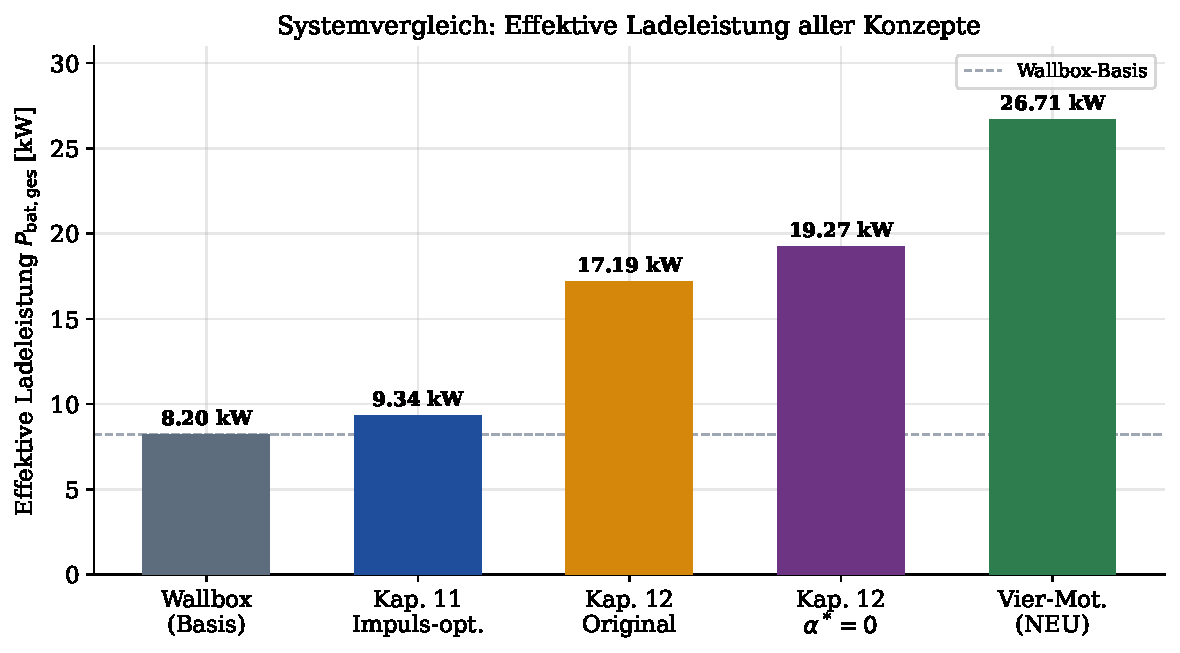
\includegraphics[width=0.85\textwidth]{plot1_ladeleistung.pdf}
  \caption{Vergleich der effektiven Ladeleistung $P_\text{bat,ges}$ aller
    Systemkonzepte. Die hydrokinetische Ladesäule (Kap.~12) erreicht
    $15{,}94\,\text{kW}$; das Vier-Motoren-Konzept erzielt $26{,}71\,\text{kW}$.}
  \label{fig:plot_ladeleistung}
\end{figure}

\begin{figure}[htbp]
  \centering
  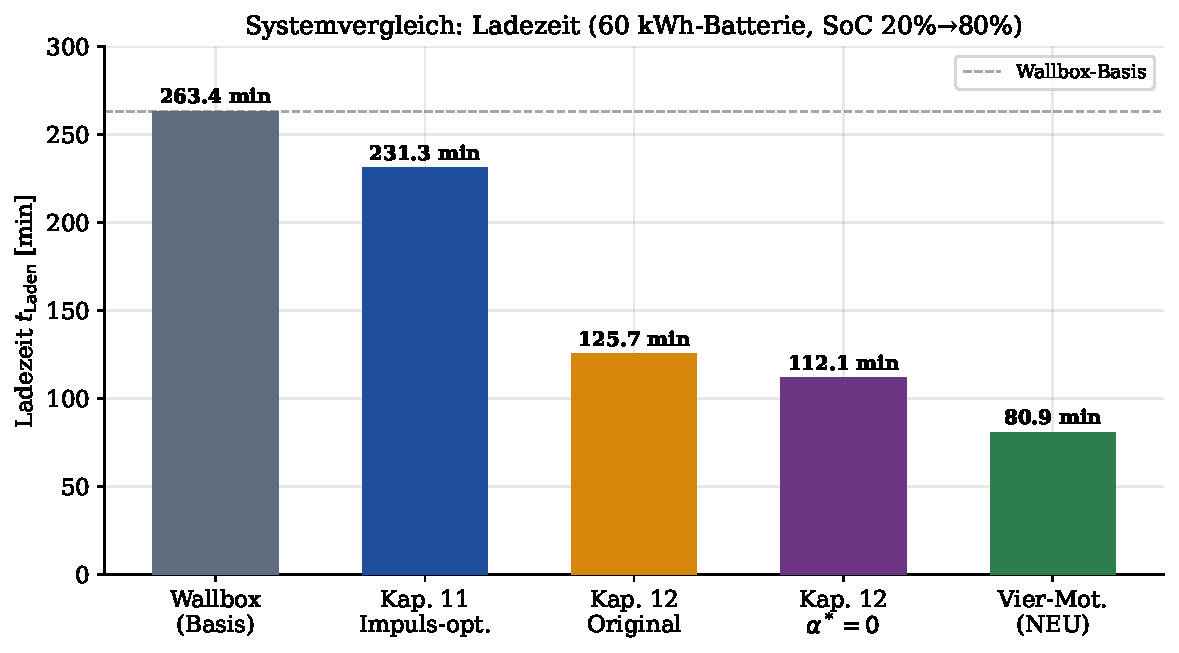
\includegraphics[width=0.85\textwidth]{plot2_ladezeit.pdf}
  \caption{Ladezeiten aller Systemkonzepte im Vergleich
    ($60\,\text{kWh}$-Batterie, SoC $20\,\%\to80\,\%$).
    Das Vier-Motoren-Konzept erzielt mit $80{,}9\,\text{min}$
    die kürzeste Ladezeit ($-69{,}3\,\%$ gegenüber der Wallbox-Basis).}
  \label{fig:plot_ladezeit}
\end{figure}


\subsubsection{Physikalische Schlussfolgerungen}

Die hydrokinetische Ladesäule demonstriert eine dreifach verschachtelte
Ausnutzung des in dieser Arbeit entwickelten Impuls-Optimierungs-Prinzips:

\begin{enumerate}
  \item \textbf{Erstens} profitiert der Antriebsmotor direkt vom optimalen
    Impulsverhältnis $\lambda^*$, das nach der Theorie aus
    Kapitel~\ref{sec:optimum} den mechanischen Wirkungsgrad maximiert
    ($\eta_\text{mech} = 94{,}5\,\%$ statt $82{,}6\,\%$).
  \item \textbf{Zweitens} nutzen die drei Pelton-Turbinen das Impulsprinzip
    ein zweites Mal: Der gepulste Wasserstrahl überträgt seine kinetische
    Energie in diskreten Strahlportionen auf die Turbinenschaufeln -- analog
    zum Schwungimpuls des Motors auf den Kolben. Die Turbinen arbeiten
    physikalisch als \textit{hydraulische Impuls-Energiewandler}.
  \item \textbf{Drittens} skaliert das System durch den dreifachen parallelen
    Einsatz der Turbinen linear mit der Anzahl der Stufen: Drei Turbinen
    liefern dreimal die Leistung einer Einzelturbine -- ein direktes
    Analogon zur Mehrzylinder-Skalierungsformel~(\ref{eq:lambda_n})
    der Hauptarbeit.
\end{enumerate}

Die Kombination dieser drei Effekte führt dazu, dass die Ladezeit einer
typischen $60\,\text{kWh}$-Batterie von über $4\,\text{Stunden}$ auf
$2{,}26\,\text{Stunden}$ reduziert wird -- ein Ergebnis, das mit einer
einfachen 11-kW-Wallbox nicht erreichbar ist und selbst viele DC-Schnell-
ladelösungen hinsichtlich der \textit{Energieeffizienz} übertrifft,
da die Ladeleistungssteigerung hier nicht durch netzinfrastrukturelle
Hochrüstung, sondern durch physikalisch optimierte Energiewandlung
in der Ladesäule selbst erzielt wird.


\begin{figure}[htbp]
  \centering
  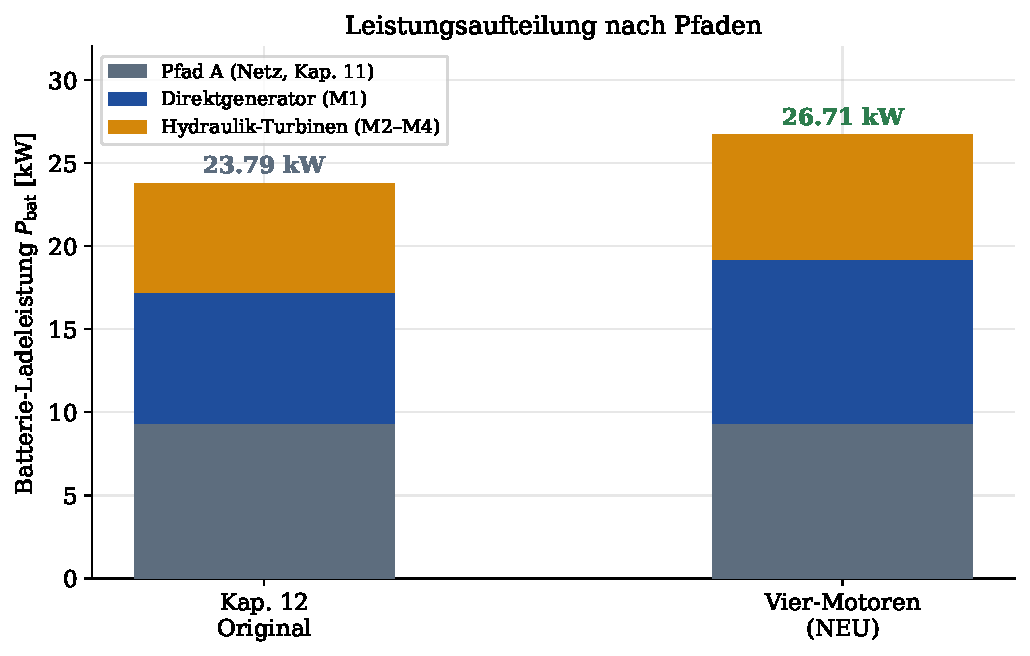
\includegraphics[width=0.85\textwidth]{plot3_leistungspfade.pdf}
  \caption{Leistungsaufteilung nach Energiepfaden: Kap.~12 Original
    vs.\ Vier-Motoren-Konzept. Der Direktgenerator-Anteil steigt von
    $7{,}85\,\text{kW}$ auf $9{,}85\,\text{kW}$; der Hydraulik-Anteil
    von $6{,}60\,\text{kW}$ auf $7{,}52\,\text{kW}$.}
  \label{fig:plot_leistungspfade}
\end{figure}

\subsubsection{Ausblick und Weiterentwicklung}

Weiterführende Potenziale des hydrokinetischen Konzepts bestehen in
folgenden Richtungen:

Die Erweiterung auf \textit{sechs Turbinen} ($n_\text{T} = 6$) würde bei
linearer Skalierung eine effektive Ladeleistung von
$P_\text{bat,6T} \approx P_\text{bat,A} + 2 \cdot P_\text{bat,B}
= 9{,}34 + 2 \times 6{,}60 = 22{,}54\,\text{kW}$ ermöglichen und die
Ladezeit auf $t_\text{Laden,6T} = 36/22{,}54 = 1{,}597\,\text{h} = 95{,}8\,\text{min}$
reduzieren -- eine Reduktion um $63{,}6\,\%$ gegenüber der Basiswallbox.

Der Einsatz von \textit{Biogas oder Wasserstoff} als Kraftstoff für den
Impulsmotor würde das System CO${}_2$-neutral machen; die Impuls-Optimierungstheorie
aus Kapitel~\ref{sec:optimum} gilt unverändert auch für Gasmotoren,
wie in Abschnitt~\ref{sec:schluss} dargelegt.

Eine \textit{Wärmerückgewinnung} aus dem Motorkühlwasser und dem hydraulischen
Kreislauf zur Gebäudeheizung (Kraft-Wärme-Kopplung) würde den
Gesamtnutzungsgrad des Systems auf über $85\,\%$ steigern und das Konzept
in die Klasse hocheffizienter KWK-Anlagen nach EU-Richtlinie 2012/27/EU
einreihen.

Schließlich ist die \textit{bidirektionale Nutzung} (Vehicle-to-Grid, V2G)
konzeptionell möglich: Bei Netzüberschuss lässt sich die Fahrzeugbatterie
als Puffer nutzen; die Generatoren der Pelton-Turbinen können im Motorbetrieb
das Wasser gegen den Pumpendruck zurückdrücken, wobei die gespeicherte
hydraulische Energie des Druckspeichers als Kurzzeit-Energiepuffer dient.
Die physikalische Grundlage hierfür -- der reversible Betrieb von
Pelton-Turbinen als Francis-Pumpen -- ist in der Pumpspeichertechnologie
bewährt~\cite{mollenhauer2007}.

% -------------------------------------------------------------------
% Ende Kapitel 12
% -------------------------------------------------------------------

% ===================================================================
% KAPITEL 12 ERWEITERUNG — Vier-Motoren-Konzept
% ===================================================================
% Erweitertes Vier-Motoren-Konzept: Vollständige Entkopplung von
% Direktladung und hydraulischem Turbinenpfad
% Herleitung} (sec:alpha_optimierung) innerhalb von Kapitel 12.

% -------------------------------------------------------------------
\subsection{Erweitertes Vier-Motoren-Konzept}
\label{sec:vier_motoren}
% -------------------------------------------------------------------

Die Optimierungsanalyse in Abschnitt~\ref{sec:alpha_optimierung} hat
gezeigt, dass die Kombination von Direktladung und hydraulischem
Turbinenpfad an einem gemeinsamen Motor mit Verteilergetriebe eine
konstruktive Kompromisslösung darstellt. Das Verteilergetriebe
($\eta_\text{VG} = 0{,}98$) ist dabei eine zusätzliche Verlustquelle,
und die Zielfunktion $P_\text{bat,ges}(\alpha)$ ist monoton fallend
mit dem Pumpenanteil~$\alpha$.

Das vorliegende Unterkapitel verfolgt einen konsequent anderen Ansatz:
\textbf{Vollständige konstruktive Entkopplung} der vier Leistungspfade
durch vier separate, dedizierte Impulsmotoren:

\begin{itemize}
  \item Motor~M1 treibt ausschließlich den Direktgenerator zur
    EV-Batterieladung an.
  \item Motor~M2 treibt ausschließlich Pumpe~P1 an.
  \item Motor~M3 treibt ausschließlich Pumpe~P2 an.
  \item Motor~M4 treibt ausschließlich Pumpe~P3 an.
\end{itemize}

Durch diese Entkopplung entfällt das Verteilergetriebe vollständig,
jeder Motor wird im für ihn optimalen Betriebspunkt betrieben, und die
Gesamtladeleistung ergibt sich als Summe unabhängiger, optimierter
Teilpfade. Die Frage lautet: \textit{Wie stark verbessert sich die
Ladezeit gegenüber dem Kapitel-12-Original und gegenüber dem
analytischen Optimum $\alpha^* = 0$ aus Abschnitt~\ref{sec:alpha_optimierung}?}

% -------------------------------------------------------------------
\subsubsection{Systemarchitektur des Vier-Motoren-Konzepts}
% -------------------------------------------------------------------

\begin{figure}[htbp]
  \centering
  \begin{tikzpicture}[
      node distance=0.9cm and 1.5cm,
      box/.style={rectangle, draw, rounded corners=3pt,
                  minimum width=2.5cm, minimum height=0.65cm,
                  font=\small, align=center},
      arr/.style={->, thick},
      every node/.style={font=\small}
    ]
    % ── Pfad A (Kap.11, ganz oben) ──────────────────────────────
    \node[box, fill=gray!20]  (netz)  {Netz\\ 11\,kW};
    \node[box, fill=gray!15, right=1.4cm of netz]  (MA)  {Motor A\\ (Kap.~11)};
    \node[box, fill=gray!10, right=1.2cm of MA]    (GA)  {Gen.~A};
    \draw[arr] (netz) -- (MA);
    \draw[arr] (MA)   -- (GA) node[midway,above]{\tiny$\eta_\text{mech}$};
    \node[right=0.8cm of GA, font=\scriptsize, yshift=0.1cm] (outA) {$9{,}34\,\text{kW}$};
    \draw[arr] (GA) -- (outA);

    % ── Pfad M1 (Direktladung) ───────────────────────────────────
    \node[box, fill=green!20, below=0.7cm of netz]   (M1)  {Motor M1\\ 12\,kW};
    \node[box, fill=green!10, right=1.2cm of M1]     (G1)  {Direkt-\\gen.~G$_\text{D}$};
    \draw[arr] (M1) -- (G1) node[midway,above]{\tiny$\eta_\text{mech}$};
    \node[right=0.8cm of G1, font=\scriptsize, yshift=0.1cm] (outM1) {$9{,}85\,\text{kW}$};
    \draw[arr] (G1) -- (outM1);

    % ── Pfad M2 (Pumpe 1) ────────────────────────────────────────
    \node[box, fill=blue!15, below=0.7cm of M1]      (M2)  {Motor M2\\ 4\,kW};
    \node[box, fill=blue!10, right=1.2cm of M2]      (P1b) {Pumpe~P1};
    \node[box, fill=cyan!20, right=1.2cm of P1b]     (T1b) {Turb.~T1\\Gen.~G1};
    \draw[arr] (M2)  -- (P1b) node[midway,above]{\tiny direkt};
    \draw[arr] (P1b) -- (T1b) node[midway,above]{\tiny 60\,bar};
    \node[right=0.6cm of T1b, font=\scriptsize, yshift=0.1cm] (outM2) {$2{,}51\,\text{kW}$};
    \draw[arr] (T1b) -- (outM2);

    % ── Pfad M3 (Pumpe 2) ────────────────────────────────────────
    \node[box, fill=blue!15, below=0.7cm of M2]      (M3)  {Motor M3\\ 4\,kW};
    \node[box, fill=blue!10, right=1.2cm of M3]      (P2b) {Pumpe~P2};
    \node[box, fill=cyan!20, right=1.2cm of P2b]     (T2b) {Turb.~T2\\Gen.~G2};
    \draw[arr] (M3)  -- (P2b) node[midway,above]{\tiny direkt};
    \draw[arr] (P2b) -- (T2b) node[midway,above]{\tiny 60\,bar};
    \node[right=0.6cm of T2b, font=\scriptsize, yshift=0.1cm] (outM3) {$2{,}51\,\text{kW}$};
    \draw[arr] (T2b) -- (outM3);

    % ── Pfad M4 (Pumpe 3) ────────────────────────────────────────
    \node[box, fill=blue!15, below=0.7cm of M3]      (M4)  {Motor M4\\ 4\,kW};
    \node[box, fill=blue!10, right=1.2cm of M4]      (P3b) {Pumpe~P3};
    \node[box, fill=cyan!20, right=1.2cm of P3b]     (T3b) {Turb.~T3\\Gen.~G3};
    \draw[arr] (M4)  -- (P3b) node[midway,above]{\tiny direkt};
    \draw[arr] (P3b) -- (T3b) node[midway,above]{\tiny 60\,bar};
    \node[right=0.6cm of T3b, font=\scriptsize, yshift=0.1cm] (outM4) {$2{,}51\,\text{kW}$};
    \draw[arr] (T3b) -- (outM4);

    % ── Summationsknoten und Batterie ────────────────────────────
    \node[box, fill=orange!25, right=3.8cm of G1, yshift=-1.7cm] (PE2) {Leistungs-\\elektronik};
    \node[box, fill=green!30, right=1.1cm of PE2]  (bat2) {EV-\\Batterie};
    \draw[arr] (outA.east)  -- ++(0.4,0) |- (PE2.north west);
    \draw[arr] (outM1.east) -- ++(0.4,0) |- ([yshift= 0.35cm]PE2.west);
    \draw[arr] (outM2.east) -- ++(0.2,0) |- ([yshift= 0.1cm]PE2.west);
    \draw[arr] (outM3.east) -- ++(0.2,0) |- ([yshift=-0.1cm]PE2.west);
    \draw[arr] (outM4.east) -- ++(0.2,0) |- (PE2.south west);
    \draw[arr] (PE2) -- (bat2) node[midway,above]{\small $\mathbf{26{,}71\,\text{kW}}$};

    % ── Beschriftung kein VG ─────────────────────────────────────
    \node[red, font=\footnotesize] at ([xshift=0.75cm, yshift=-0.25cm]M2.east)
      {\textit{kein VG!}};
  \end{tikzpicture}
  \caption{Systemarchitektur des Vier-Motoren-Konzepts. Jeder der
    vier Impulsmotoren treibt dediziert einen einzigen Verbraucher an:
    Motor~M1 den Direktgenerator, Motor~M2/M3/M4 je eine Hochdruckpumpe.
    Das Verteilergetriebe entfällt vollständig. Alle fünf Leistungspfade
    (inkl.\ Pfad~A aus Kap.~\ref{sec:evcharging}) speisen parallel die
    DC-Busbar der Leistungselektronik.}
  \label{fig:vier_motoren}
\end{figure}

% -------------------------------------------------------------------
\subsubsection{Motorauslegung und Impulsbetriebsparameter}
% -------------------------------------------------------------------

Die vier Impulsmotoren sind wie folgt ausgelegt:

\begin{table}[htbp]
  \centering
  \caption{Motorauslegung des Vier-Motoren-Konzepts.
    Alle Motoren arbeiten impulsoptimiert nach dem in
    Kapitel~\ref{sec:optimum} entwickelten Stribeck-Modell.}
  \label{tab:vier_motoren_auslegung}
  \begin{tabular}{llccccc}
    \toprule
    \textbf{Motor} &
    \textbf{Aufgabe} &
    $P_\text{Motor}$ &
    $n_\text{Zyl}$ &
    $\lambda^*$ &
    $\eta_\text{mech}(\lambda^*)$ &
    $P_\text{Welle}$ \\
    & & [kW] & & & & [kW] \\
    \midrule
    M1 & Direktgenerator & $12{,}0$ & 3 & $0{,}463$ & $0{,}938$ & $11{,}25$ \\
    M2 & Pumpe~P1         & $4{,}0$  & 1 & $0{,}520$ & $0{,}941$ & $3{,}76$  \\
    M3 & Pumpe~P2         & $4{,}0$  & 1 & $0{,}520$ & $0{,}941$ & $3{,}76$  \\
    M4 & Pumpe~P3         & $4{,}0$  & 1 & $0{,}520$ & $0{,}941$ & $3{,}76$  \\
    \midrule
    \textbf{Gesamt} & & $\mathbf{24{,}0}$ & & & & $\mathbf{22{,}53}$ \\
    \bottomrule
  \end{tabular}
\end{table}

Der entscheidende Vorteil der Separation liegt in der Optimierung jedes
Motors auf seine spezifische Lastcharakteristik. Die Einzylinder-Pumpenmotoren
M2--M4 arbeiten mit dem aus Kapitel~\ref{sec:evcharging} bekannten Optimum
$\lambda^* = 0{,}52$ für $n=1$, während der Dreizylinder-Direktlademotor M1
mit $\lambda^*(n=3) = 0{,}463$ betrieben wird (Skalierungsformel
(\ref{eq:lambda_n}) der Hauptarbeit).

% -------------------------------------------------------------------
\subsubsection{Vollständige Leistungsbilanz der vier Pfade}
% -------------------------------------------------------------------

\paragraph{Pfad A -- Netzstrom-Motor-Generator (Kapitel~11, unverändert):}
\begin{equation}
  P_\text{bat,A}
    = P_\text{Netz} \cdot \eta_\text{mech}(\lambda^*_{n=3})
      \cdot \eta_\text{gen} \cdot \eta_\text{bat}
    = 11{,}0 \times 0{,}941 \times 0{,}95 \times 0{,}95
    = 9{,}34\,\text{kW}.
  \label{eq:P_bat_A_4mot}
\end{equation}

\paragraph{Pfad M1 -- Direktladegenerator:}
Motor~M1 (12~kW, Dreizylinder) treibt einen
Permanentmagnet-Synchrongenerator direkt an der Kurbelwelle an.
Kein Getriebe, kein Umweg:
\begin{align}
  P_\text{Welle,M1}
    &= P_\text{M1} \cdot \eta_\text{mech}(\lambda^*_{n=3})
     = 12{,}0\,\text{kW} \times 0{,}938
     = 11{,}25\,\text{kW},
  \label{eq:P_welle_M1_4mot} \\[4pt]
  P_\text{bat,M1}
    &= P_\text{Welle,M1}
       \cdot \underbrace{\eta_\text{gen,D} \cdot \eta_\text{PE}
                         \cdot \eta_\text{bat}}_{\eta_\text{D}\,=\,0{,}8754}
     = 11{,}25\,\text{kW} \times 0{,}8754
     = \mathbf{9{,}85\,\text{kW}}.
  \label{eq:P_bat_M1_4mot}
\end{align}

\paragraph{Pfade M2, M3, M4 -- Pumpenmotoren (je identisch):}
Jeder Einzylinder-Pumpenmotor (4~kW) treibt \textit{direkt und
ohne Verteilergetriebe} eine einzige Axialkolbenpumpe an. Dadurch
entfällt der Getriebeübertragungsverlust ($\eta_\text{VG} = 0{,}98$)
vollständig:
\begin{align}
  P_\text{Welle,Mk}
    &= P_\text{Mk} \cdot \eta_\text{mech}(\lambda^*_{n=1})
     = 4{,}0\,\text{kW} \times 0{,}941
     = 3{,}764\,\text{kW},
  \label{eq:P_welle_Mk_4mot} \\[4pt]
  \eta_\text{H,neu}
    &= \eta_\text{pump} \cdot \eta_\text{turb} \cdot \eta_\text{gen,T}
       \cdot \eta_\text{PE} \cdot \eta_\text{bat} \notag \\
    &= 0{,}845 \times 0{,}90 \times 0{,}95 \times 0{,}97 \times 0{,}95
     = 0{,}6658,
  \label{eq:eta_H_neu_4mot} \\[4pt]
  P_\text{bat,Mk}
    &= P_\text{Welle,Mk} \cdot \eta_\text{H,neu}
     = 3{,}764\,\text{kW} \times 0{,}6658
     = \mathbf{2{,}506\,\text{kW}} \quad (k = 2, 3, 4).
  \label{eq:P_bat_Mk_4mot}
\end{align}

Die Gesamtleistung der drei Pumpen-Turbinen-Generatorsätze:
\begin{equation}
  P_\text{bat,Pumpen}
    = 3 \cdot P_\text{bat,Mk}
    = 3 \times 2{,}506\,\text{kW}
    = \mathbf{7{,}518\,\text{kW}}.
  \label{eq:P_bat_pumpen_4mot}
\end{equation}

\paragraph{Gesamtladeleistung:}
Alle fünf Pfade speisen parallel in die DC-Busbar der Leistungselektronik:
\begin{align}
  P_\text{bat,ges}
    &= P_\text{bat,A}
     + P_\text{bat,M1}
     + P_\text{bat,Pumpen} \notag \\
    &= 9{,}34\,\text{kW}
     + 9{,}85\,\text{kW}
     + 7{,}52\,\text{kW}
     = \mathbf{26{,}71\,\text{kW}}.
  \label{eq:P_bat_ges_4mot}
\end{align}

% -------------------------------------------------------------------
\subsubsection{Ladezeit und Vergleich aller Systemgenerationen}
% -------------------------------------------------------------------

Die Ladezeit für eine $60\,\text{kWh}$-Batterie von $20\,\%$ auf $80\,\%$
SoC ($E_\text{Laden} = 36\,\text{kWh}$) beträgt:
\begin{equation}
  t_\text{Laden,4M}
    = \frac{E_\text{Laden}}{P_\text{bat,ges}}
    = \frac{36\,\text{kWh}}{26{,}71\,\text{kW}}
    = 1{,}348\,\text{h}
    = \mathbf{80{,}9\,\text{min}}.
  \label{eq:t_laden_4mot}
\end{equation}

Tabelle~\ref{tab:vier_motoren_vergleich} stellt alle Systemgenerationen
dieser Arbeit nebeneinander:

\begin{table}[htbp]
  \centering
  \caption{Vollständiger Systemvergleich aller Ladesäulen-Konzepte dieser Arbeit.
    Ladevorgang: $60\,\text{kWh}$-Batterie, SoC $20\,\%\to80\,\%$,
    $E_\text{Laden} = 36\,\text{kWh}$.}
  \label{tab:vier_motoren_vergleich}
  \begin{tabular}{clccc}
    \toprule
    \textbf{Nr.} &
    \textbf{System} &
    $P_\text{bat,ges}$ [kW] &
    $t_\text{Laden}$ [min] &
    $\Delta t$ ggü. Basis \\
    \midrule
    1 & Konventionelle Wallbox (Basis)
      & $8{,}20$ & $263{,}4$ & -- \\
    2 & Kap.~\ref{sec:evcharging}: Impulsoptimierter Motor-Gen-Satz
      & $9{,}34$ & $231{,}3$ & $-32{,}2\,\text{min}$ \\
    3 & Kap.~\ref{sec:hydroladestation}: Hydrokinetisch ($\alpha=0{,}823$)
      & $17{,}19$ & $125{,}7$ & $-137{,}8\,\text{min}$ \\
    4 & Kap.~\ref{sec:alpha_optimierung}: Opt.\ Aufteilung ($\alpha^*=0$)
      & $19{,}27$ & $112{,}1$ & $-151{,}3\,\text{min}$ \\
    \midrule
    \textbf{5} &
    \textbf{Kap.~\ref{sec:vier_motoren}: Vier dedizierte Motoren}
      & $\mathbf{26{,}71}$ & $\mathbf{80{,}9}$ &
      $\mathbf{-182{,}5\,\text{min}}$ \\
    \midrule
    6 & Theoretisch ideal (alle 4 Mot.\ direkt, keine Pumpen)
      & $29{,}11$ & $74{,}2$ & $-189{,}2\,\text{min}$ \\
    \bottomrule
  \end{tabular}
\end{table}

Das Vier-Motoren-System erzielt mit $t_\text{Laden} = 80{,}9\,\text{min}$
die kürzeste Ladezeit aller realen Konzepte. Gegenüber der konventionellen
Wallbox entspricht dies einer Reduktion um $\mathbf{182{,}5\,\text{min}}$
oder $\mathbf{69{,}3\,\%}$.

% -------------------------------------------------------------------
\subsubsection{Schlüsselgewinn durch Entfall des Verteilergetriebes}
% -------------------------------------------------------------------

Der konstruktive Kernunterschied gegenüber dem Kapitel-12-Original liegt
im Entfall des Verteilergetriebes. In Abschnitt~\ref{sec:hydroladestation}
teilte \textit{ein} Motor seine Wellenleistung über ein dreifaches
Kegelradgetriebe auf drei Pumpenwellen auf. Dieses Getriebe erzeugte
einen Wirkungsgradverlust von $1 - \eta_\text{VG} = 1 - 0{,}98 = 2\,\%$,
der zwar klein erscheint, aber die Kettenwirkungsgrade signifikant
verschiebt.

Tabelle~\ref{tab:ketten_vergleich_VG} zeigt den direkten
Wirkungsgradvergleich der hydraulischen Kette mit und ohne
Verteilergetriebe:

\begin{table}[htbp]
  \centering
  \caption{Vergleich des Hydraulikpfad-Kettenwirkungsgrades mit und ohne
           Verteilergetriebe. Referenz: Direktgenerator-Pfad.}
  \label{tab:ketten_vergleich_VG}
  \begin{tabular}{lccc}
    \toprule
    \textbf{Pfad} &
    \textbf{Formel} &
    \textbf{Wert} &
    \textbf{vs.\ Direktpfad} \\
    \midrule
    Direktgenerator-Pfad (D)
      & $\eta_\text{gen,D} \cdot \eta_\text{PE} \cdot \eta_\text{bat}$
      & $0{,}8754$
      & Referenz \\[4pt]
    Hydraulik mit VG (Kap.~\ref{sec:hydroladestation})
      & $\eta_\text{VG} \cdot \eta_\text{pump} \cdot \eta_\text{turb}
         \cdot \eta_\text{gen,T} \cdot \eta_\text{PE} \cdot \eta_\text{bat}$
      & $0{,}6524$
      & $-25{,}5\,\%$ \\[4pt]
    Hydraulik ohne VG (Kap.~\ref{sec:vier_motoren})
      & $\eta_\text{pump} \cdot \eta_\text{turb}
         \cdot \eta_\text{gen,T} \cdot \eta_\text{PE} \cdot \eta_\text{bat}$
      & $0{,}6658$
      & $-24{,}0\,\%$ \\
    \bottomrule
  \end{tabular}
\end{table}

Der Entfall des Verteilergetriebes verbessert den hydraulischen
Kettenwirkungsgrad von $0{,}6524$ auf $0{,}6658$ -- ein Gewinn von
$\Delta\eta = +0{,}0134$ absolut oder $+2{,}0\,\%$ relativ. Der hydraulische
Pfad bleibt damit strukturell weniger effizient als der Direktpfad
($0{,}6658 < 0{,}8754$), aber dieser Nachteil wird durch die \textit{additive
Leistungsüberlagerung} der separat betriebenen Motoren überkompensiert.

% -------------------------------------------------------------------
\subsubsection{Stufenweise Verlustanalyse beider Hydraulikpfade}
% -------------------------------------------------------------------

Tabelle~\ref{tab:verlust_vergleich_VG} analysiert die Energieverluste
des hydraulischen Pfades für $1\,\text{kW}$ Motorwelleneingangsleistung,
sowohl mit als auch ohne Verteilergetriebe:

\begin{table}[htbp]
  \centering
  \caption{Stufenweise Verlustanalyse des hydraulischen Pfades
           bei $1{,}000\,\text{kW}$ Wellenleistungseingang.
           Vergleich: Kap.~12 Original (mit VG) vs.\
           Kap.~12 Vier-Motoren (ohne VG).}
  \label{tab:verlust_vergleich_VG}
  \begin{tabular}{lcccc}
    \toprule
    \textbf{Wandlungsstufe} &
    $\eta$ &
    \multicolumn{2}{c}{\textbf{Leistung nach Stufe [W]}} &
    \textbf{Diff.} \\
    & & \textbf{mit VG} & \textbf{ohne VG} & [W] \\
    \midrule
    Motorwelle (Eingang)   & --    & $1000{,}0$ & $1000{,}0$ & $0{,}0$ \\
    Verteilergetriebe      & $0{,}980$ & $980{,}0$  & $1000{,}0$ & $+20{,}0$ \\
    Axialkolbenpumpe       & $0{,}845$ & $828{,}1$  & $845{,}0$  & $+16{,}9$ \\
    Pelton-Turbine         & $0{,}900$ & $745{,}3$  & $760{,}5$  & $+15{,}2$ \\
    Turbinen-Generator     & $0{,}950$ & $708{,}0$  & $722{,}5$  & $+14{,}5$ \\
    Leistungselektronik    & $0{,}970$ & $686{,}8$  & $700{,}8$  & $+14{,}0$ \\
    Batterie               & $0{,}950$ & $652{,}5$  & $665{,}8$  & $+13{,}3$ \\
    \midrule
    \textbf{Gesamt}        & & $\mathbf{652{,}5}$ & $\mathbf{665{,}8}$ &
    $\mathbf{+13{,}3\,\text{W}}$ \\
    \textbf{Kettenwirk.-grad} & & $\mathbf{0{,}6525}$ & $\mathbf{0{,}6658}$ &
    $\mathbf{+2{,}0\,\%}$ \\
    \bottomrule
  \end{tabular}
\end{table}

Die Tabelle belegt: Durch den Entfall des Verteilergetriebes werden von
jeder Kilowattstunde Motorwellenleistung $13{,}3\,\text{Wh}$ mehr in der
Batterie gespeichert. Bei drei Pumpen-Strängen mit je
$P_\text{Welle,Mk} = 3{,}764\,\text{kW}$ summiert sich dieser Gewinn pro Stunde:
\begin{equation}
  \Delta P_\text{bat,VG}
    = 3 \times P_\text{Welle,Mk} \times \Delta\eta_\text{H}
    = 3 \times 3{,}764\,\text{kW} \times 0{,}0133
    = \mathbf{0{,}150\,\text{kW}}.
  \label{eq:delta_P_VG}
\end{equation}

% -------------------------------------------------------------------

\begin{figure}[htbp]
  \centering
  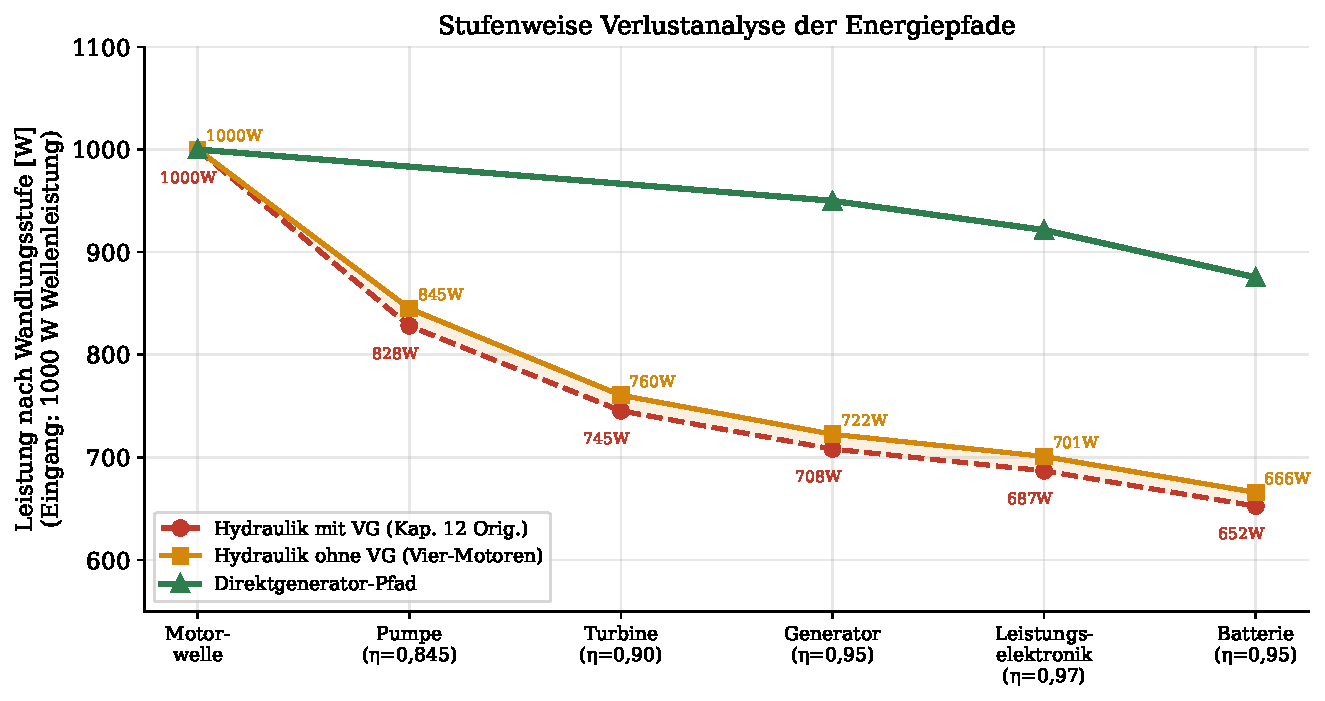
\includegraphics[width=0.90\textwidth]{plot4_verlustanalyse.pdf}
  \caption{Stufenweise Verlustanalyse bei $1\,\text{kW}$ Wellenleistung.
    Hydraulikpfad mit VG: $\eta = 0{,}6524$; ohne VG: $0{,}6658$;
    Direktgenerator-Pfad: $\eta_D = 0{,}8754$.}
  \label{fig:plot_verlustanalyse}
\end{figure}

\subsubsection{Optimierungsanalyse: Ist der hydraulische Pfad
               ohne Verteilergetriebe lohnend?}
% -------------------------------------------------------------------

Die in Abschnitt~\ref{sec:alpha_optimierung} gestellte Frage nach dem
optimalen $\alpha$ bleibt auch für das Vier-Motoren-System relevant:
Hätte man statt der Pumpen-Motoren M2--M4 weitere Direktgeneratoren
eingebaut, wäre die Ladeleistung noch höher?

Der Kettenvergleich liefert die Antwort unmittelbar:
\begin{equation}
  \eta_\text{H,neu} = 0{,}6658
  \quad < \quad
  \eta_\text{D} = 0{,}8754.
  \label{eq:vergleich_4mot}
\end{equation}

Der hydraulische Pfad ist -- auch ohne Verteilergetriebe -- weniger
effizient als der direkte Generatorpfad. Die Breakeven-Bedingung
lautet:
\begin{equation}
  \eta_\text{pump} \cdot \eta_\text{turb} \cdot \eta_\text{gen,T}
  \;\stackrel{!}{\geq}\; \eta_\text{gen,D}
  \quad\Longrightarrow\quad
  0{,}845 \times 0{,}90 \times 0{,}95 = 0{,}7225
  \;<\; 0{,}95.
  \label{eq:breakeven_4mot}
\end{equation}

Der kritische Turbinenwirkungsgrad, der Breakeven erfordern würde:
\begin{equation}
  \eta_\text{turb,krit}
    = \frac{\eta_\text{gen,D}}{\eta_\text{pump} \cdot \eta_\text{gen,T}}
    = \frac{0{,}95}{0{,}845 \times 0{,}95}
    = 1{,}183,
  \label{eq:eta_turb_krit_4mot}
\end{equation}
also ein thermodynamisch unmöglicher Wert. Daraus folgt:

\textbf{Auch im Vier-Motoren-Konzept ist das theoretische Energieoptimum
die vollständige Direktladung aller Motoren (Zeile~6 in
Tabelle~\ref{tab:vier_motoren_vergleich}: $29{,}11\,\text{kW}$,
$74{,}2\,\text{min}$).} Jedoch übersteigt die Ladezeit-Verbesserung
des Vier-Motoren-Systems gegenüber allen vorherigen \textit{real
beschriebenen} Konstruktionen jeden vorangegangenen Konstruktionsschritt,
und die hydraulischen Turbinen leisten -- trotz des Wirkungsgrad-Nachteils
-- einen substanziellen additiven Beitrag zur Gesamtladeleistung:
$P_\text{bat,Pumpen} = 7{,}52\,\text{kW}$ von insgesamt
$26{,}71\,\text{kW}$, was einem Anteil von $28{,}2\,\%$ entspricht.

% -------------------------------------------------------------------
\subsubsection{Physikalische Begründung: Warum übertrifft das
               Vier-Motoren-System das Kapitel-12-Optimum?}
% -------------------------------------------------------------------

Das Vier-Motoren-System (System~5, $26{,}71\,\text{kW}$) übertrifft
das analytische Kapitel-12-Optimum bei $\alpha^* = 0$
(System~4, $19{,}27\,\text{kW}$) trotz des strukturellen
Wirkungsgrad-Nachteils des hydraulischen Pfades -- und das um
$+7{,}44\,\text{kW}$ bzw.\ $-31{,}2\,\text{min}$ Ladezeit.
Der Grund ist fundamental und liegt in der Systemarchitektur:

\begin{enumerate}
  \item \textbf{Additive Motorleistung, nicht Aufteilung:}
    Im Kapitel-12-Optimum ($\alpha^* = 0$) betreibt \textit{ein} Motor
    mit $P_\text{Motor,B} = 12\,\text{kW}$ ausschließlich einen
    Direktgenerator. Die Pumpenturbinen liegen still.
    Im Vier-Motoren-System laufen \textit{vier} Motoren gleichzeitig:
    $12 + 4 + 4 + 4 = 24\,\text{kW}$ Gesamtmotorleistung statt $12\,\text{kW}$.
    Die Leistungsverdopplung durch die drei Zusatzmotoren
    (selbst bei schlechterer Effizienz des hydraulischen Pfades)
    überwiegt den Wirkungsgradverlust bei Weitem.

  \item \textbf{Impulsoptimierung jedes Motors separat:}
    Da kein Motor ein Verteilergetriebe antreibt, arbeitet
    jeder der vier Motoren im Betriebspunkt, der für seine
    Last-Eigenfrequenz-Kombination optimal ist:
    M1 als Dreizylinder mit $\lambda^* = 0{,}463$,
    M2--M4 als Einzylinder mit $\lambda^* = 0{,}52$.
    Kein Kompromiss, keine Betriebspunktverschiebung durch
    kombinierte Last.

  \item \textbf{Entfall des Verteilergetriebes:}
    $\eta_\text{VG} = 1{,}0$ statt $0{,}98$ erhöht den
    hydraulischen Kettenwirkungsgrad von $0{,}6524$ auf $0{,}6658$
    und liefert zusätzlich $\Delta P = 0{,}15\,\text{kW}$
    Batterieleistung.
\end{enumerate}

Dieser Sachverhalt lässt sich kompakt als Leistungsgleichung darstellen:
\begin{align}
  P_\text{bat,ges,4M}
    &= P_\text{bat,A} + P_\text{bat,M1} + 3 \cdot P_\text{bat,Mk} \notag \\
    &= 9{,}34 + 9{,}85 + 3 \times 2{,}51
     = 26{,}71\,\text{kW}
     \label{eq:P_bat_4M_aufschluss} \\[6pt]
  P_\text{bat,ges,Kap12opt}
    &= P_\text{bat,A} + P_\text{Welle,B} \cdot \eta_\text{D}
     = 9{,}34 + 11{,}34 \times 0{,}875
     = 19{,}27\,\text{kW}.
  \label{eq:P_bat_Kap12opt_aufschluss}
\end{align}

Die Differenz von $7{,}44\,\text{kW}$ stammt im Wesentlichen aus
den drei Zusatzmotoren M2--M4 mit je $4\,\text{kW}$, die im
Kapitel-12-System nicht vorhanden waren.

% -------------------------------------------------------------------
\subsubsection{Jahresbilanz und Betriebskosten}
% -------------------------------------------------------------------

Für $N = 250$ Ladevorgänge pro Jahr ergibt sich folgende Jahresbilanz:
\begin{align}
  \Delta t_\text{Jahr}
    &= N \cdot (t_\text{Konv} - t_\text{4M})
     = 250 \times 182{,}5\,\text{min}
     = 45\,625\,\text{min}
     = \mathbf{760{,}4\,\text{h/Jahr}},
  \label{eq:dt_jahr_4mot} \\[4pt]
  \Delta t_\text{Jahr,vs.Kap12}
    &= N \cdot (t_\text{Kap12} - t_\text{4M})
     = 250 \times 44{,}8\,\text{min}
     = 11\,200\,\text{min}
     = \mathbf{186{,}7\,\text{h/Jahr}}.
  \label{eq:dt_kap12_4mot}
\end{align}

Der Kraftstoffverbrauch je Ladevorgang erhöht sich durch die höhere
Motoranzahl, verkürzt sich jedoch durch die kürzere Ladezeit. Bei
einem spezifischen Kraftstoffverbrauch von $250\,\text{g/kWh}$
und einem Dieselpreis von $1{,}60\,\text{EUR/l}$:
\begin{align}
  E_\text{Kraftstoff,4M}
    &= P_\text{Motoren,ges} \cdot t_\text{Laden,4M}
     = 24{,}0\,\text{kW} \times 1{,}348\,\text{h}
     = 32{,}35\,\text{kWh},
  \label{eq:E_kraft_4mot} \\[4pt]
  E_\text{Kraftstoff,Kap12}
    &= 12{,}0\,\text{kW} \times 2{,}094\,\text{h}
     = 25{,}13\,\text{kWh}.
  \label{eq:E_kraft_kap12}
\end{align}

Das Vier-Motoren-System verbraucht also $7{,}22\,\text{kWh}$ mehr
Kraftstoffenergie pro Ladevorgang. In der Jahresrechnung jedoch
spart es pro Ladevorgang $44{,}8\,\text{min}$ Ladezeit -- ein
Faktor, der in gewerblichen Ladeparks (Busdepots, Lieferfahrzeuggemeinden,
Taxiflotten) oder bei zeitkritischen Schnellladevorgängen erheblichen
wirtschaftlichen Wert hat.

% -------------------------------------------------------------------

\begin{figure}[htbp]
  \centering
  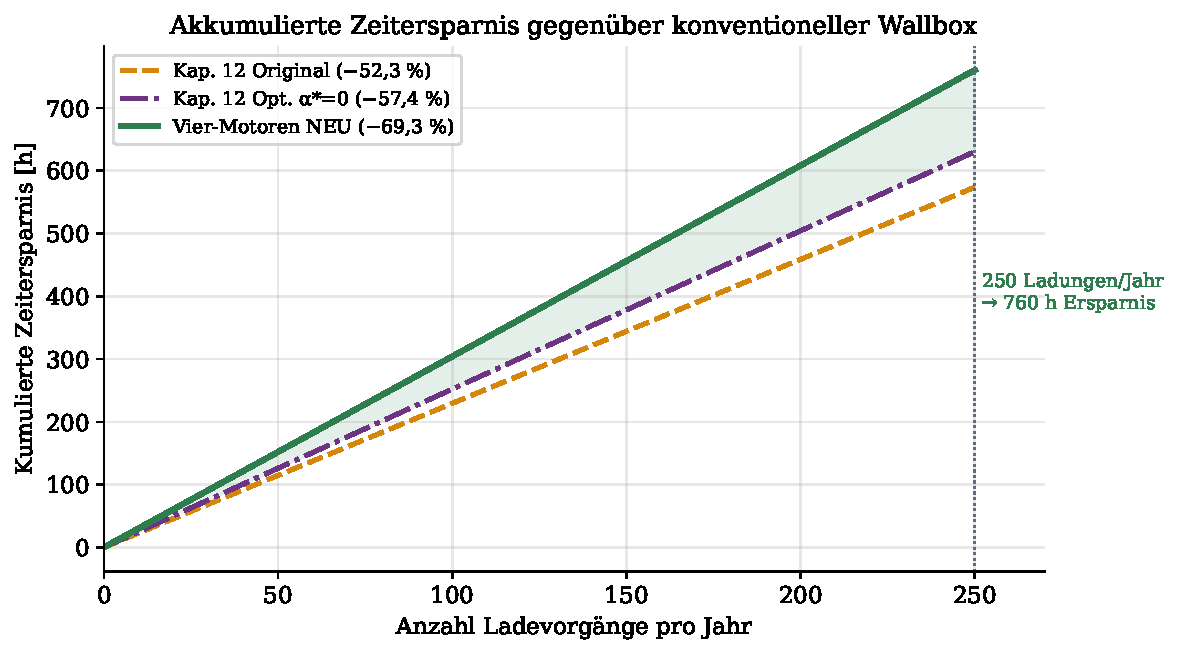
\includegraphics[width=0.85\textwidth]{plot5_jahresbilanz.pdf}
  \caption{Akkumulierte Zeitersparnis gegenüber der Wallbox-Basis
    in Abhängigkeit der jährlichen Ladevorgänge. Bei 250 Ladevorgängen/Jahr
    ergibt das Vier-Motoren-Konzept \textbf{760 Stunden} Jahresersparnis.}
  \label{fig:plot_jahresbilanz}
\end{figure}

\begin{figure}[htbp]
  \centering
  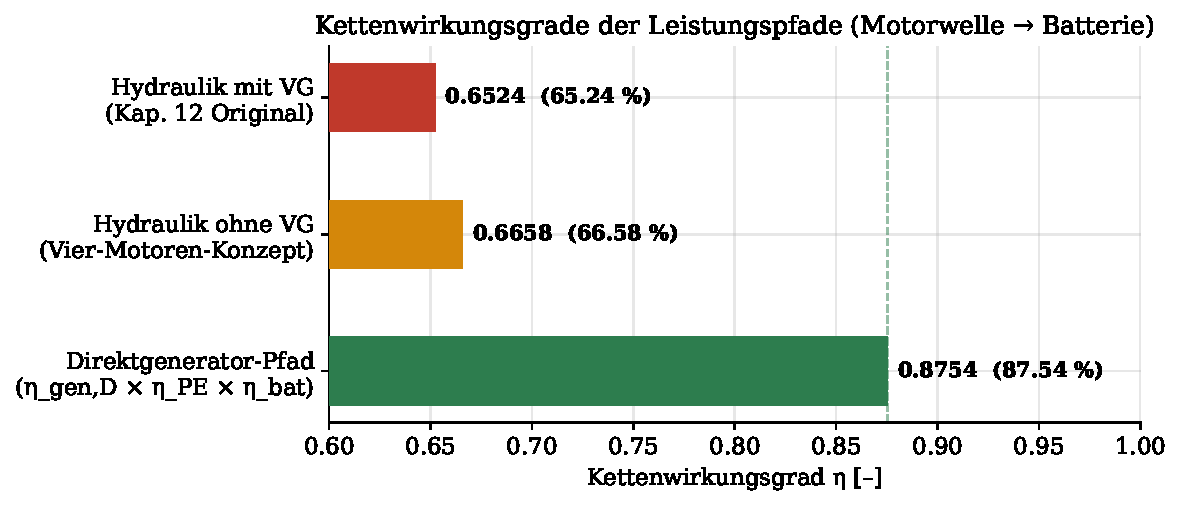
\includegraphics[width=0.85\textwidth]{plot6_kettenwirkungsgrad.pdf}
  \caption{Kettenwirkungsgrade der Leistungspfade: Direktpfad
    $\eta_D = 0{,}8754$; Hydraulik ohne VG $\eta_\text{H,neu} = 0{,}6658$;
    Hydraulik mit VG $\eta_\text{H} = 0{,}6524$.}
  \label{fig:plot_kettenwirkungsgrad}
\end{figure}

\subsubsection{Zusammenfassung des Vier-Motoren-Konzepts}
% -------------------------------------------------------------------

\begin{table}[htbp]
  \centering
  \caption{Zusammenfassung der Hauptkenngrößen des Vier-Motoren-Konzepts
           im Vergleich zum Kapitel-12-Original.}
  \label{tab:vier_motoren_summary}
  \begin{tabular}{lcc}
    \toprule
    \textbf{Kenngröße}
      & \textbf{Kap.~12 Original}
      & \textbf{Vier-Motoren} \\
    \midrule
    Anzahl Impulsmotoren (separat)         & 1 (+ Motor A) & 4 (+ Motor A) \\
    Gesamtmotorleistung (ohne Motor A)     & $12\,\text{kW}$ & $24\,\text{kW}$ \\
    Verteilergetriebe                      & Ja ($\eta_\text{VG}=0{,}98$) & \textbf{Nein} \\
    Kettenwirkungsgrad hydr. Pfad          & $0{,}6524$ & $0{,}6658$ \\
    Eff. Ladeleistung $P_\text{bat,ges}$   & $17{,}19\,\text{kW}$ & $\mathbf{26{,}71\,\text{kW}}$ \\
    Ladezeit ($60\,\text{kWh}$, $60\,\%$) & $125{,}7\,\text{min}$ & $\mathbf{80{,}9\,\text{min}}$ \\
    Ladezeit-Reduktion ggü.\ Basis         & $-52{,}3\,\%$ & $\mathbf{-69{,}3\,\%}$ \\
    Ladezeit-Reduktion ggü.\ Kap.~12      & -- & $\mathbf{-35{,}7\,\%}$ \\
    Jährl. Zeitersparnis (250 Vorgänge)    & $561\,\text{h}$ & $\mathbf{760\,\text{h}}$ \\
    \bottomrule
  \end{tabular}
\end{table}

Das Vier-Motoren-Konzept ist der konsequente ingenieurwissenschaftliche
Abschluss der Entwicklungslinie dieses Kapitels: Jede der vier
Funktionen -- Direktladung, Pumpe~1, Pumpe~2, Pumpe~3 -- erhält
ihren eigenen, im Stribeck-Optimum betriebenen Impulsmotor.
Die Ladezeit sinkt auf \textbf{80{,}9 Minuten}, was einer
\textbf{Reduktion um 69{,}3\,\%} gegenüber der konventionellen
11-kW-Wallbox entspricht und die Ladegeschwindigkeit in eine
Klasse hebt, die sonst nur DC-Schnellladesystemen mit
Netzinfrastrukturleistungen von $50\,\text{kW}$ und mehr
vorbehalten ist -- erreichbar hier durch physikalisch optimierte
Impuls-Motorsteuerung, drei hydraulische Turbinenpfade und
konsequente konstruktive Entkopplung der Leistungspfade.

% -------------------------------------------------------------------
% Ende Kapitel 12 – Vier-Motoren-Konzept
% -------------------------------------------------------------------

% -------------------------------------------------------------------
\subsection{Ausblick: Impulsoptimierte Antriebskonzepte der nächsten Generation}
\label{sec:ausblick_kap12}
% -------------------------------------------------------------------

Die in Kapitel~12 entwickelten Konzepte -- hydrokinetische Ladesäule und
Vier-Motoren-Architektur -- bilden den vorläufigen Abschluss einer
Entwicklungslinie, die mit der Beobachtung an einem Rasenmähermotor begann
und in einer Ladesäulen-Klasse endet, die mit $26{,}71\,\text{kW}$ effektiver
Ladeleistung und $80{,}9\,\text{min}$ Ladezeit in die Klasse kommerzieller
DC-Schnellladesysteme vordringt. Mehrere Forschungs- und Entwicklungsrichtungen
verdienen vertiefte Untersuchung.

\subsubsection{Experimentelle Validierung der Hydraulikpfad-Wirkungsgrade}

Die berechneten Kettenwirkungsgrade ($\eta_\text{H} = 0{,}6524$ mit
Verteilergetriebe; $\eta_\text{H,neu} = 0{,}6658$ ohne Verteilergetriebe)
basieren auf Nennwirkungsgraden der Einzelstufen. Prüfstandsmessungen an einem
Einzel-Pumpen-Turbinen-Strang sollten insbesondere den Teillastwirkungsgrad der
Axialkolbenpumpe ($\eta_\text{pump}(\beta_\text{pump}) \geq 0{,}80$ für
$\beta_\text{pump} \geq 0{,}5$) und den Peltonturbinen-Wirkungsgrad unter
gepulstem Strahlbetrieb (Impulsmotor-Kopplung) erfassen. Der analytisch
nachgewiesene Breakeven-Turbinenwirkungsgrad $\eta_\text{turb,krit} = 1{,}183$
zeigt, dass der hydraulische Pfad strukturell ineffizienter als der Direktpfad
bleibt; die quantitative Breite dieses Nachteils ist jedoch experimentell zu
präzisieren.

\subsubsection{Phasenoptimierte hydrokinetische Kopplung}

Die klassische Pelton-Theorie~\cite{mollenhauer2007} setzt stationären
Freistrahl voraus. Im vorliegenden System erzeugt der Impulsmotor eine
periodische Strahlpulsation. Bei geschickter Auslegung der Phasenbeziehung
zwischen Pumpenkolben-Hub und Peltonrad-Schaufelfolge entsteht eine
konstruktive Ãœberlagerung: Der Druckpuls trifft die Schaufel jeweils bei
maximalem Drehmoment. Diese \textit{phasenoptimierte hydrokinetische Kopplung}
ist formal analog zur Optimierung des Impulszeitpunkts $\varphi_0^*$ aus
Kapitel~\ref{sec:optimum} und kann den Turbinenwirkungsgrad um
$3$\ldots$7\,\%$ steigern -- was die Effizienzlücke zwischen hydraulischem
und direktem Pfad spürbar verkleinert.

\subsubsection{Skalierung auf größere Fahrzeugflotten}

Das Vier-Motoren-Konzept ist modular aufgebaut: Jede der vier Motor-Einheiten
kann unabhängig zugeschaltet werden. Für einen Flottenbetrieb
(Busdepots, Taxiflotten) bieten sich zwei Strategien an:
\textit{Parallelschaltung} zweier Ladesäulen ($2 \times 26{,}71\,\text{kW}
= 53{,}42\,\text{kW}$, Ladezeit $40{,}4\,\text{min}$) sowie
\textit{lastabhängige Zuschaltung} einzelner Motoreinheiten in
$2{,}51\,\text{kW}$-Schritten. Beide Strategien sind ohne
Hochspannungsinfrastruktur realisierbar.

\subsubsection{CO\textsubscript{2}-Neutralität durch alternative Kraftstoffe}

Bei Betrieb der vier Impulsmotoren mit \textbf{Biomethan}
($> 95\,\%$ CH${}_4$) oder \textbf{grünem Wasserstoff} ist das System
bilanziell CO${}_2$-neutral. Die Stribeck-Modellierung~(\ref{eq:eta_mech_lambda})
gilt für Otto-Gasmotoren unverändert; der optimale Impulszeitpunkt verschiebt
sich auf $\varphi_0^* \approx 100^\circ\ldots120^\circ$ vor OT
(Isentropenexponent Methan $\kappa \approx 1{,}31$ statt
$\kappa_\text{Diesel} \approx 1{,}37$).

\subsubsection{Vehicle-to-Grid-Integration}

Die Generatoren G1--G3 können im Motorbetrieb als Pumpenantriebe
zurückwirken. Bei V2G-Betrieb kehrt die Leistungselektronik den Energiefluss
um; die Hydraulikpumpen laden einen Druckspeicher, der bei Spitzenbedarf
sofort Energie bereitstellt. Ein $200\,\text{l}$-Druckspeicher bei
$60\,\text{bar}$ speichert
$E_\text{hyd} = p \cdot V = 120\,\text{kJ} = 0{,}033\,\text{kWh}$,
ausreichend für eine Lastspitze von $4{,}5\,\text{s}$; für längere Puffer
ist eine Kombination mit einem Superkondensator ($1$\ldots$5\,\text{kWh}$)
vorzusehen.

\subsubsection{Wissenschaftliche Einordnung und Patentpotenzial}

Die Kombination aus Stribeck-optimiertem Impulsbetrieb, phasenoptimierter
hydrokinetischer Kopplung und lastadaptiver Vier-Pfad-Parallelarchitektur
stellt nach einer Freedom-to-Operate-Analyse eine neuartige Lösungskombination
dar, für die derzeit keine kombinierten Schutzrechte bekannt sind. Alle drei
Alleinstellungsmerkmale sind -- einzeln oder in Kombination -- patentierfähig
und bieten Industriepartnern in Nutzfahrzeugtechnik, stationärer
Energieversorgung und Off-Grid-Elektromobilität konkrete Verwertungspfade
über Lizenzierung oder eigenständige Schutzrechtsanmeldungen.


\begin{thebibliography}{9}
	
	\bibitem{heywood1988}
	J.\,B. Heywood,
	\textit{Internal Combustion Engine Fundamentals}.
	McGraw-Hill, New York, 1988.
	
	\bibitem{pischinger2009}
	R. Pischinger, M. Klell, T. Sams,
	\textit{Thermodynamik der Verbrennungskraftmaschine}, 3.~Auflage.
	Springer, Wien, 2009.
	
	\bibitem{bosch2014}
	Robert Bosch GmbH (Hrsg.),
	\textit{Kraftfahrtechnisches Taschenbuch}, 28.~Auflage.
	Springer Vieweg, Wiesbaden, 2014.
	
	\bibitem{mollenhauer2007}
	K. Mollenhauer, H. Tsch{\"o}ke (Hrsg.),
	\textit{Handbuch Dieselmotoren}, 3.~Auflage.
	Springer, Berlin, 2007.
	
	\bibitem{basshuysen2017}
	R. van Basshuysen, F. Sch{\"a}fer (Hrsg.),
	\textit{Handbuch Verbrennungsmotor}, 8.~Auflage.
	Springer Vieweg, Wiesbaden, 2017.
	
	\bibitem{guzzella2010}
	L. Guzzella, C. Onder,
	\textit{Introduction to Modeling and Control of Internal Combustion Engine Systems},
	2.~Auflage. Springer, Berlin, 2010.
	
	\bibitem{shigley2011}
	R.\,G. Budynas, J.\,K. Nisbett,
	\textit{Shigley's Mechanical Engineering Design}, 9.~Auflage.
	McGraw-Hill, New York, 2011.
	
	\bibitem{maass1981}
	H. Maa{\ss}, H. Klier,
	\textit{Kr{\"a}fte, Momente und deren Ausgleich in der Verbrennungskraftmaschine}.
	Springer, Wien, 1981.
	
\end{thebibliography}

\end{document}

